\documentclass[a4paper,12pt, oneside]{report}
\usepackage[hyphens]{url}
\usepackage[style=apa, backend=biber, urldate=long, uniquename=false]{biblatex}
\DeclareLanguageMapping{british}{british-apa}
\addbibresource{bibliography.bib}
\usepackage[british]{babel}
\usepackage{hyperref}
\usepackage[top=1in, left=1.5in, right=1in, bottom=1in]{geometry}
\usepackage[utf8]{inputenc}
\usepackage[usenames,dvipsnames]{color}
\usepackage{setspace}
\usepackage{titlepic}
\usepackage{graphicx}
\usepackage[nodayofweek]{datetime}
\usepackage{float}
\usepackage{booktabs}
\usepackage{tablefootnote}
\usepackage{multirow}
\usepackage{csquotes}
\usepackage{setspace}

% Ordinals and numbering
\usepackage[super]{nth}
\usepackage[gen]{eurosym}

%Plots with Latex
\usepackage{pgfplots}
%change the size of each plot and also guarantee compatibility backwards
\pgfplotsset{width=12cm,compat=1.9}
%required to work with full dates
\usepgfplotslibrary{dateplot}

%Changing main font
\usepackage{mathpazo}

% Subscripts - defining new command
\newcommand{\textunderscript}[1]{$_{\textup{#1}}$}

% Change fontsize of figures
\usepackage[font=footnotesize,labelfont=bf]{caption}

% Change for table on layers
\usepackage{longtable}

%% Style
%% Paragraph settings
\setlength{\parskip}{0.9em}

% Checkmarks
\usepackage{tikz}
\def\checkmark{\tikz\fill[scale=0.4](0,.35) -- (.25,0) -- (1,.7) -- (.25,.15) -- cycle;} 

%for CC
\newcommand*\circled[1]{\tikz[baseline=(char.base)]{\node[shape=circle,draw,inner sep=0.6pt](char){#1};}}

% Allows to add subsubsections
\usepackage{titlesec}
\setcounter{secnumdepth}{4}
\titleformat{\paragraph}
{\normalfont\normalsize\bfseries}{\theparagraph}{1em}{}
\titlespacing*{\paragraph}
{0pt}{3.25ex plus 1ex minus .2ex}{1.5ex plus .2ex}

%Make footnotes global
\usepackage{chngcntr}
\counterwithout{footnote}{chapter}

% Headers
\usepackage{fancyhdr}

% Fancy chapter heading
\usepackage[Bjornstrup]{fncychap}
 \renewcommand{\headrulewidth}{1.5pt}
 
\usepackage[acronym, nonumberlist, nopostdot]{glossaries}

% Package to deal with appendices
\usepackage[toc,page]{appendix}
 
\makeglossaries

%%%%%%%%%%%%%%%%%%%%%%%%%%%
%%%%%%%% ACRONYMS %%%%%%%%%%%%%
\newacronym{cbpp}{CBPP}{Commons-Based Peer Production}
\newacronym{floss}{FLOSS}{Free/Libre Open Source Software}
\newacronym{mit}{MIT}{Massachusetts Institute of Technology}
\newacronym{fsf}{FSF}{Free Software Foundation}
\newacronym{gnu}{GNU}{GNU's Not Unix (recursive acronym)}
\newacronym{osi}{OSI}{Open Source Initiative}
\newacronym{vcs}{VCS}{Version Control System}
\newacronym{dvcs}{DVCS}{Distributed Version Control System}
\newacronym{ekm}{EKM}{Extended Klandermans Model}
\newacronym{vist}{VIST}{Valence, Instrumentality, Self-efficacy, Trust}
\newacronym{php}{PHP}{PHP: Hypertext Preprocessor (recursive acronym)}
\newacronym{gpl}{GPL}{General Public License}
\newacronym{cms}{CMS}{Content Management System}
\newacronym{fosdem}{FOSDEM}{Free and Open Source Software Developers' European Meeting}
\newacronym{f2f}{F2F}{Face-to-face}
\newacronym{osuol}{OSUOL}{Oregon State University Open Source Lab}
\newacronym{it}{IT}{Information Technology}
\newacronym{nasa}{NASA}{National Aeronautics and Space Administration}
\newacronym{at}{AT}{Activity Theory}
\newacronym{gnome}{GNOME}{GNU Network Object Model Environment}
\newacronym{sql}{SQL}{Structured Query Language}
\newacronym{ssh}{SSH}{Secure SHell}
\newacronym{css}{CSS}{Cascading Style Sheet}
\newacronym{html}{HTML}{Hypertext Markup Language}
\newacronym{ux}{UX}{User Experience}
\newacronym{pdf}{PDF}{Portable Document Format}
\newacronym{caqdas}{CAQDAS}{Computer Assisted Qualitative Data Analysis Software}
\newacronym{irc}{IRC}{Internet Relay Chat}
\newacronym{oscom}{OSCOM}{Open Source CMS Conference}
\newacronym{cc}{CC}{Creative Commons}
\newacronym{cvs}{CVS}{Concurrent Versioning System}
\newacronym{url}{URL}{Uniform Resource Locator}
\newacronym{api}{API}{Application Program Interface}
\newacronym{rtbc}{RTBC}{Reviewed and Tested By the Community}
\newacronym{pap}{PAP}{Project Application Process}
\newacronym{bdfl}{BDFL}{Benevolent Dictator For Life}
\newacronym{bof}{BoF}{Birds of a Feather}
\newacronym{na}{N/A}{Not Applicable}
\newacronym{adsl}{ADSL}{Asymmetric Digital Subscriber Line}
\newacronym{ant}{ANT}{Actor-Network Theory}

%%%%%%%%%%%%%%%%%%%%%%%%%%%

%Fixing issue with padding on ToF
\makeatletter
\renewcommand\@pnumwidth{2.2em}
\makeatother

\begin{document}

\thispagestyle{empty}
\begin{center}
\begin{minipage}{0.95\textwidth}
    \centering
    {\huge \textbf{Self-organisation in Commons-Based  Peer Production}\par}
    \vspace{0.5cm}
    {\Large \textbf{Drupal: ``the drop is always moving"}\par}
    \vspace{0.75cm}
    {\Large by\par}
    \vspace{0.75cm}
    {\Large David Rozas\par}
    \vspace{1.5cm}
    
     %University logo
    \includegraphics[width=0.3\linewidth]{img/surrey_logo.png}
    \vspace{2cm}
   
 {\large 
                    Submitted for the Degree of Doctor of Philosophy \\
                    \vspace{0.5cm}
 					Centre for Research in Social Simulation \\
					Department of Sociology\\
					Faculty of Arts and Social Sciences\\
					University of Surrey\\}
   \vspace{1cm}
    {\large Supervisors: \\
					Prof. Nigel Gilbert\\
					Dr Paul Hodkinson\\
	}

    \vspace{1cm}  
    \vspace{0.5cm} 
    {\small {\scriptsize \circled{\reflectbox{\textbf{C}}}} David Rozas 2017}
\end{minipage}
\end{center}
\clearpage

\onehalfspacing
%%% SECTIONS WITH EMPTY STYLE %%%%%%
\pagestyle{empty}

%% Declaration
\newpage
\section*{Declaration}

This thesis and the work to which it refers are the results of my own efforts. Any ideas, data, images or
text resulting from the work of others (whether published or unpublished) are fully identified as such
within the work and attributed to their originator in the text, bibliography or in footnotes. This thesis
has not been submitted in whole or in part for any other academic degree or professional qualification.
I agree that the University has the right to submit my work to the plagiarism detection service
TurnitinUK for originality checks. Whether or not drafts have been so-assessed, the University reserves
the right to require an electronic version of the final document (as submitted) for assessment as above.

\vspace{.6in}
Signature:


\vspace{.6in}


Date:


\vspace{4.5cm}

\par\noindent\rule{\textwidth}{0.4pt}

\hspace{2.9cm}
\begin{minipage}[b]{0.75\linewidth}
\begin{flushright}
{\small 

\textbf{Word count: 96,873.}\\

This work was partially supported by the Framework programme FP7 ICT-2013-10 of the European Commission through project \href{http://www.p2pvalue.eu/}{P2Pvalue} (grant no.: 610961).
It is licensed under a \href{https://creativecommons.org/licenses/by-sa/4.0/}{Creative Commons Attribution-ShareAlike 4.0 International}.\\
A digital version of this work and its source files (\LaTeX) can be found at \url{https://davidrozas.cc/phd}. 
}

\vspace{0.5cm}

\includegraphics[width=1.5in]{img/CC-BY-SA_icon.png} 

\end{flushright}
\end{minipage}

\newpage
\begin{flushright}
\vspace*{2cm}
\large{\textit{A mis padres, os quiero.}}
\end{flushright}

%% Abstract
\newpage
\input{sections/abstract}

%Acknowledgement
\newpage
\section*{Acknowledgments}

This thesis signifies the most challenging and enthralling intellectual journey of my life. Or, perhaps, a sum of multiple journeys. A multidisciplinary journey, from Computer Science to Sociology. An epistemological journey, from an engineering-shaped mind towards the use of qualitative methods as a tool of immense power to further our understanding of certain questions. An enlightening journey, from participating in free software communities to realising the complexity that lies behind them, and embarking on a quest to understand this complexity as part of the wider phenomenon of Commons-Based Peer Production.  

This journey would never have been possible without the confidence placed on me by Professor Nigel Gilbert, my main supervisor. I met Nigel five years ago when I attended a talk he gave at the Universidad Complutense about a research project named QScience, partly developed on Drupal, which I found by chance in a free software social news website. I became really interested in the research he was leading and I decided to approach him with some more questions after his talk. Luckily for me, he told me they were looking for a Drupal developer and I decided to apply. Weeks later I moved to the UK to work with him as part of the project. I always dreamt of having the opportunity to study a PhD and I felt the dream was closer after being nearer to an academic environment. A few months later, I asked him whether I could refer to him in a PhD application I was preparing, to which he kindly agreed. Some days later he asked me whether I would be interested in doing the PhD at the University of Surrey under his supervision. I still cannot describe the tremendous happiness and honour I felt, and still feel, in that precise moment. I would like to express my most sincere admiration and gratitude for providing me with the opportunity to work together with a scientist of such standing over the past years. His confidence and advice have constantly empowered me in this journey and challenge of becoming a researcher.

This thesis would be a completely different piece of work without the invaluable advice and countless enlightened conversations with Dr Paul Hodkinson, my co-supervisor. My epistemological journey and my passion for increasing my knowledge of Sociology would have never been possible without his mentorship and help. I would like to express my most sincere gratitude for his support and for his time and interest in discussing and supervising my research. 

This research took place in the Centre for Research and Social Simulation (CRESS), the most multidisciplinary and international working environment I have ever had the chance to be in. The innumerous inspiring conversations I had with my colleagues in CRESS over these years deeply enriched this work. But, most importantly, the truly multidisciplinary and diverse environment of CRESS widened my understanding of Science and helped me improve my critical thinking. I would also like to give a special mention for my colleague Dr David Anzola, whose friendship started the moment I joined CRESS and remained even after he finished his PhD and moved back to Colombia, and which I am sure will remain for the rest of our lives. I would also like to thank the researchers from the \textit{Centro Studi di Etnografia Digitale} in Milano and GRASIA in Madrid, who hosted me as a visiting fellow while conducting this research. The brilliant minds and inspiring conversations I had with the researchers of these groups have made an invaluable contribution to this work.

In addition, I would like to thank all of my colleagues from the P2Pvalue project, whose collaboration and inspiration have made me grow as a researcher. The P2Pvalue project funded three of the four years of my research, but most importantly it provided an invaluable opportunity to become involved in and study the world of the commons with some of the most bright, knowledgeable and passionate minds devoted to further our understanding of this phenomenon. I truly hope to continue to contribute to this research field in my future career and to maintain my collaboration and friendship with all of my P2Pvalue colleagues.

I would also like to sincerely thank the Drupal community. What Drupal represents to this work goes beyond a simple case study. Drupal is a community of passionate women and men to create a technology which provides freedom to their users, and shows us how cooperation can triumph over competition. I would also like to thank more specifically all of the Drupalistas with whom I crossed paths for their help to make this research possible, and a special mention must be made to all the informants and interviewees who participated in this research. I would also like to thank more specifically the local communities of London and Madrid, for welcoming me in and helping me with this research as well as in my path to become a Drupalista.

Special thanks are devoted to all the friends I met after moving to Guildford. They provided me with emotional support and we had great moments together: Ana, Sacha, Marianna, Sandra, Belén, Jaime, Pepe, María, Tone, Stephy and so many others! I really hope our paths keep crossing. I would also like to thank the love and support received by my friends in Madrid. A more concrete mention must be made for my closest friends in Madrid: Raúl (now Dr Serrano!) and Antonio. We found each other more than twenty years ago, we grew up together, and in a way we shaped, and keep shaping, each other intellectually. My passion for aiming to untangle the complexity behind any social phenomenon and my critical thinking would have probably never developed in this way without the countless hours we have spent discussing politics, philosophy, history, sociology or technology in the parks of my hometown, Alcorcón. I would also like to thank Blanca for her encouragement to start this journey in times when I was coping with impostor syndrome, and her constantly present emotional support in spite of the physical distance which separated us once I moved to the UK. I also cannot forget to mention Loba, my wonderful dog, who I adopted more than a year ago, just a day after returning back to Madrid. She was sitting next to me in my home office while I was writing most of this work. I still cannot find the words to describe the love and loyalty received by her every day.

I also thank the love and support received from my family, who I always felt next to me in spite of the distance. I especially thank my parents, to whom I dedicate this thesis. I profoundly missed them every single day during the four years I spent in the UK, and I thank them for their constant encouragement, comprehension and love, as well as for all their work and efforts to raise and educate me to become the person I am, with my attributes and flaws. I love you.

Finally, I would like to thank my life partner Tabi. We found each other on a train from Guildford to London two years ago, while I was re-reading Levy's ``Hackers" for this thesis. That initial conversation on the train led to the discovery of a fascinating, caring and loving mind which I hope to keep exploring for the rest of my life. I do not think I could ever have completed this journey without her encouragement and determination over the past two years, which is well illustrated by  the writing she made on my whiteboard, \textit{¡Sí se puede!}, which I could never erase until concluding this thesis. She has been the closest person to accompany me during this amusing journey: the countless hours she spent proofreading this work, the numerous stimulating conversations about the research, and her constant care, love and support cannot be properly thanked with simple words. Neither can I find words descriptive enough to capture the impact she had on my life the moment we found each other. Thus, I can only thank her by expressing my feelings towards her: \textit{te quiero, dormilona}.

%%% END SECTIONS WITH EMPTY STYLE %%%%%%

%%% Regular style starts here
\clearpage
\pagestyle{fancy}
\fancyhf{}
\fancyhead[RE,LO]{\slshape \nouppercase \leftmark}
\fancyhead[LE,RO]{\thepage}

%% Print index 
\newpage
\setcounter{tocdepth}{1} 
\tableofcontents
\setcounter{tocdepth}{1} %to solve issue with appendixes affecting list of figs and tables

%% Print list of figures and tables
\newpage
\listoftables
\newpage
\listoffigures

%Print list of acronyms
\glsaddallunused
\printglossary[type=\acronymtype, title=List of acronyms]

%%%%%%%% CHAPTERS %%%%%%%%%%%%

% A 3-4 pages preface introducing the topic and the relevance
\setcounter{chapter}{-1}
\chapter{Preface}
\chaptermark{Preface}
\label{chapter:preface}

This study is contextualised under the massive technological, social, political and economic changes experienced over the past twenty years, in which the lines between consumers and producers have become more blurred. This phenomenon has been labelled using the term collaborative economy: an umbrella concept which encompasses disparate initiatives which range from Wikipedia, a free encyclopedia written collaboratively and collectively owned; to Uber, a corporation-owned platform connecting drivers and passengers. Over the course of the years in which this study took place (2013-2017), the collaborative economy has been permeating into more and more aspects of our lives and has been receiving significantly increasing interest far beyond academia. The impact of corporation-owned platforms on diminishing labour rights is nowadays, for example, a common debate in mass media \parencite[e.g.][]{bbc-collab:2017:Online, elpais-collab:2017:Online}. The term collaborative economy has become a priority in the agenda of political institutions \parencite[e.g.][]{euc-collab:2017:Online, generalitatcollab2017}, which is seen as a source of new opportunities and innovation, but also as a source of tensions between previous market operators and the new actors. The rise of the collaborative economy is also employed as an indicator of a systemic contradiction leading to a zero marginal cost economy, in which some authors \parencite[e.g.][]{bauwens2014communism, mason2016postcapitalism} envision the practices from some of the initiatives of the collaborative economy as a key driving force for a possible transition towards a communitarian post-capitalist system.

As recently argued by some scholars \parencite{mayo-unicorns:2017:Online}, significantly different models are emerging around collaborative economy. On the one hand, models in which the value is captured by large corporations which control the platform, communities are dis-empowered and kept out of decision-making, and the technologies and knowledge are proprietary and closed. Uber or AirBnB, a platform connecting people willing to rent rooms or whole properties to guests, are perhaps the most well-known examples of initiatives representing these \textit{corporation-based} models of collaborative economy. On the other hand, models which revolve around a \textit{commons-based} collaborative economy, in which the participants of the community own and self-organise the platform, use and develop technologies that respect the rights of their users, and share the knowledge which has been collaboratively built. Wikipedia or GNU/Linux, a Free/Libre Open Source operating system, are perhaps the most well-known examples of the initiatives around these \textit{commons-based} models. 

This thesis presents a study of self-organisation in a collaborative community focussed on the development of a Free/Libre Open Source Software, named Drupal, whose model responds to the latter: a \textit{Commons-Based} Peer Production community. Drupal is a content management framework, a software to develop web applications, which currently powers more than 2\% of websites worldwide. Since the source code, the computer instructions, was released under a license which allow its use, copy, study and modification by anyone in 2001, the Drupal project has attracted the attention of hundreds of thousands of participants. More than 1.3 million people are registered on Drupal.org, the main platform of collaboration, and communitarian events are held every week all around the World. Thus, as the main slogan of the Drupal project reflects --- ``come for the software, stay for the community", this collaborative project cannot be understood without exploring its community, which is the main focus of this thesis.

In sum, over the course of the next eleven chapters, this thesis presents the story of how hundreds of thousands of participants in a large and global Commons-Based Peer Production community have organised themselves, in what started as a small and amateur project in 2001. This is with the aim of furthering our understanding of how, coping with diverse challenges, Commons-Based Peer Production communities govern and scale up their self-organisational processes.

Chapter \ref{chapter:introduction} provides an overview of the phenomenon of Free/Libre Open Source Software and connects it with that of Commons-Based Peer Production, allowing the theoretical pillars from previous studies on both phenomena to be drawn on. Chapter \ref{chapter:case-study} provides an overview of the main case study, the Drupal community. Throughout the second chapter the Drupal community is framed as an extreme case study of Commons-Based Peer Production on the basis of its growth, therefore offering an opportunity to improve our understanding of how self-organisational processes emerge, evolve and scale up over time in Commons-Based Peer Production communities of this type.

Chapter \ref{sec:theoretical-frameworks} provides an overview of Activity Theory and its employment as an analytical tool: a lens which supports the analysis of the changes experienced in complex organisational activities, such as those from Free\slash Libre Open Source Software communities as part of the wider phenomenon of Commons-Based Peer Production. Subsequently, chapter \ref{chapter:methods}, explores the fundamental methodological aspects considered for this study, which draws on an ethnographic approach. The decision for this approach is reasoned on the basis of the nature of the research questions tackled in the study. Firstly, on requiring an inductive approach, which entails the assumption that topics emerge from the process of data analysis rather than vice versa. Secondly, on the necessity of drawing on a methodological approach which acknowledges the need to understand these topics from within the community.

Chapter \ref{identifyng-contribution:chapter} begins the presentation of the findings of this study. Concretely, it presents the findings regarding the study of contribution in the Drupal community, a notion which is fundamental for the choice of the main unit of analysis, contribution activity, in Activity Theory. The results from this study enabled the identification and consideration, throughout the subsequent chapters, not only of activities which are ``officially" understood as contributions, such as those listed in the main collaboration platform, but also of those which have remained less visible in Free/Libre Open Source software and Commons-Based Peer Production communities and the literature on them.

Having carried out this exploration of the notion of contribution in the Drupal community, the conceptual underpinnings necessary to carry out the study of self-organisation in the Drupal community, by focussing on contribution activities, are laid out. More precisely, chapters \ref{sec:custom-to-contrib} and \ref{chapter:core-system} address the study of the development of projects, activities whose main actions and operations are mostly performed through an online medium;  while chapters \ref{mostly-offline-local:chapter} and \ref{mostly-offline-cons:chapter}, the organisation of events, whose main actions and operations are mostly performed through an offline medium. Throughout these chapters the main argument that binds this thesis together is presented: the growth experienced by the Drupal community led to a formalisation of self-organisational processes in response to a general dynamic of decentralisation of decision-making in order for these processes to scale up. This research identified these two general organisational dynamics, formalisation and decentralisation of decision-making, affecting large and global Commons-Based Peer Production communities as they grow over time. Thus, throughout these chapters, the means by which these general dynamics of formalisation and decentralisation shaped the overall systems which emerged around these different contribution activities are explored. The exploration of the organisational processes of this case study does not only show the existence of these dynamics, but it provides an in-depth account of how these dynamics relate to each other, as well as how they shaped the overall resulting system of peer production, despite the main medium of the peer production activities studied being online/offline, or the significant differences with regard to their main focus of action --- writing source code or organising events. For each pair of chapters this exploration starts with the most informal systems and progresses towards the most formal respectively: \textit{custom}, \textit{contributed} and \textit{core} projects, in chapters \ref{sec:custom-to-contrib} and \ref{chapter:core-system}; and local events, \textit{DrupalCamps} and \textit{DrupalCons}, in chapters \ref{mostly-offline-local:chapter} and \ref{mostly-offline-cons:chapter}.

After carrying out this in-depth exploration of self-organisation, the overall identified changes experienced in the self-organisational processes of the Drupal community are brought together according to general theories of self-organising communities, organisational theory and empirical studies on Commons-Based Peer Production communities, in order to connect the exploration with macro organisational aspects in chapter \ref{multilevel:chapter}. This chapter argues that this study provides evidence of the emergence of \textit{polycentric} governance, in which the participants of this community establish a constant process of negotiation to distribute authority and power over several centres of governance with effective coordination between them. In addition, this chapter argues that the exploration carried out throughout the previous chapters provides an in-depth account of the emergence of an organisational system for peer production in which different forms of organisation, varying in their degree of \textit{organicity}, simultaneously co-exist and interact with each other. Finally, chapter \ref{conclusion:chapter} summarises the main contributions of this thesis and provides a set of implications for practitioners of Commons-Based Peer Production communities.

%% Central ideas and concepts of the thesis regarding CBPP and FLOSS
\chapter{Free\slash Libre Open Source Software and Commons-Based Peer Production}
\chaptermark{FLOSS and CBPP}
\label{chapter:introduction}

This chapter provides an overview of the main areas studied in this thesis: Free\slash Libre Open Source Software and Commons-Based Peer Production.

Firstly, it will explain how informal practices to share software provided a space for the experimentation of new models of collaborative development of software fostered by the spread of the Internet. Section \ref{subsec:state-art:floss} provides a historical overview of Free\slash Libre Open Source Software, whilst providing an introduction to central concepts in this field, such as hacker culture, the differences between free software and open source software and the consequences of its growth. Section \ref{subsubsec:state-art:floss:academic-research} concludes the introduction to Free\slash Libre Open Source Software with a literature review of the main research carried out on this subject from the perspectives of a diverse range of disciplines.

Secondly, this chapter will focus on the extension of some of the principles underpinning Free\slash Libre Open Source Software in different areas, such as collaborative writing, open ecology and open design. This section provides an overview of Commons-Based Peer Production, an emergent new mode of production, the expansion of which has been of interest to many researchers. Section \ref{subsec:state-art:cbpp} provides an overview of the history of Commons-Based Peer Production and discussions about its delimitation criteria with the aim of introducing the relevant theoretical underpinnings when considering the main case study of this thesis. The case study is part of this emergent mode of production, and will be considered not only as a Free\slash Libre Open Source Software community, but as a Commons-Based Peer Production community. Finally,  section \ref{sec:cbpp-research} concludes the introduction to Commons-Based Peer Production with a review of the most recent literature on this new area of research, focussing on research that highlights the governance and organisational aspects behind Commons-Based Peer Production.

\section{Free\slash Libre Open Source Software}
\label{subsec:state-art:floss}

\subsection{Origins and commodification of the informal practice of software-sharing}
\label{subsec:origins-floss}

Free\slash Libre Open Source Software refers to software that allows its use, copy, study and modification in any way. Its origin can be found in informal practices for sharing source code: sets of computer instructions which dictate how a computer programme works in a language which is understandable by humans. The informal practice of sharing software and its source code was predominant during the 1950s and 1960s, a time when source code was not yet perceived as a commodity \parencite{deibel2013open, deibel2014open}. This practice was based on open and cooperative principles influenced by academic culture, one of the most relevant sectors producing software at the the time. The source code was typically distributed together with the software to facilitate, for example, solving errors or bugs\footnote{A bug is an error in the software which produces an unexpected result.}, or adapting it to the needs of those interested in that software. Drawing on a cooking metaphor, \textcite[17]{stallman2002free}, a key figure in the history of the free software movement, recalls the main essence of this informal culture of software-sharing in the early 1970s from his personal experience:

\begin{quotation}
``When I started working at the MIT Artificial Intelligence Lab in 1971, I became
part of a software-sharing community that had existed for many years. Sharing of
software was not limited to our particular community; it is as old as computers, just
as sharing of recipes is as old as cooking. [...]

We did not call our software `free software', because that term did not yet exist;
but that is what it was. Whenever people from another university or a company
wanted to port and use a program, we gladly let them. If you saw someone using
an unfamiliar and interesting program, you could always ask to see the source code,
so that you could read it, change it, or cannibalize parts of it to make a new program."
\end{quotation}

However, in 1969 IBM initiated a change in the way technology was commercialised. They decided to unbundle software and hardware, selling them as separate components \parencite{ibm:2014:Online}, starting a process of commodification of source code \parencite{deibel2013open, deibel2014open}. Other hardware and software producers followed and halted the distribution of source code together with the software. This process of commodification quickly spread in the 1970s \parencite{fsf-gnu-overview:2014:Online}. As part of the process, the practice of imposing legal restrictions on source code also became common, including clauses that prohibited its copy, modification, study and/or distribution. As a consequence, although the practice of software-sharing remained informal, in the early 1980s most software was proprietary \parencite{fsf-gnu-overview:2014:Online}. This shift affected all types of software, including critical components to support basic computer functions such as operating systems: the software that allows the communication between the hardware and other software. For example, the operating system Unix \parencite{unix:2014:Online} was distributed free of cost to academic and government researchers, but without permission to be modified or redistributed \parencite[128-136]{kelty2008two}.

\subsection{Hacker culture and the rise of the free software movement}
\label{subsec:hacker}

The shift towards the commodification of source code was interpreted by some computer enthusiasts as an attack on users' freedoms. The shift generated controversies about software copyright and the meanings of public domain and re-usability of software in the 1970s, such as in the case of the text editor Emacs\footnote{Emacs is a set of free/libre text editors, whose development started in 1972 at the Artificial Intelligence Lab of the MIT \parencite{emacs:Online}, which is popular for its high level of extensibility.} \parencite[189-209]{kelty2008two}. These debates were especially important between hacker communities, a sub-culture originated at the MIT during the 1950s and 1960s \parencite{levy1984hackers}. These groups were composed of computer enthusiasts who engaged in computing related activities to tackle intellectual challenges to study, understand, improve and play with technical systems. It is important to understand the term `hacker' in this context, and not by the misconception extended in mass-media of someone who exploits security vulnerabilities to attack or gain access to information systems. This type of hacker is known by hackers as ``crackers" or ``black hat hackers" \parencite[17-25]{holt2013hackers}. The work of \textcite{levy1984hackers} captures the essence of the hacker ethic, which had a great influence on the philosophy of an emerging movement in defence of what will later be known as free software, and remains fundamental to understanding the culture of free software communities, such as the free software community explored in this thesis. The hacker ethic was summarised by \textcite[26--36]{levy1984hackers}, in ``Hackers: heroes of the computer revolution":

\begin{itemize}
	\item \textit{``Access to computers --- and anything which might teach you something about the way the world works --- should be unlimited and total. Always yield to the Hands-On Imperative!"}: referring to the belief that having access to the systems will encourage hackers to learn about, play with and modify them, hence facilitating the creation of innovative, new technologies.
	\item \textit{``All information should be free"}: referring to the need to have free access to information in order to fix it and improve it. For instance, in the case of source code, this enables greater creativity and prevents wasting time in re-inventing the wheel, so everybody can benefit from it and perform improvements.
	\item \textit{``Mistrust authority --- promote decentralization"}: referring to the belief that bureaucratised systems should be avoided, since they are based on arbitrary rules to consolidate power, and they represent a threat for the creative impulse of hackers. Instead, power should be decentralised. Hackers believe open systems are the best way to promote decentralisation, since they facilitate the free exchange of information. 
	\item \textit{``Hackers should be judged by their hacking, not criteria such as degrees, age, race, sex, or position"}: referring to the meritocratic system encouraged in hacker communities, on the basis of their technical skills. For example, in the case of software development, by judging the quality of the source code instead of the superficial values of who wrote it.
	\item \textit{``You can create art and beauty on a computer"}: referring to an appreciation for innovative techniques and the aesthetics of programming style. For example, due to the limited memory space of computers at the time, there was a culture of appreciation for techniques that allowed the development of software to carry out complicated tasks in as few lines of source code as possible, or creating more efficient algorithms. 
	\item \textit{``Computers can change your life for the better"}: referring to the belief that computers have enriched their lives by looking at new forms of interacting with them.
	\item \textit{``Like Aladdin's lamp, you could get it to do your bidding"}: referring to the belief that everyone should benefit from this experience. Hackers argue that their ethic should be spread, and, because of this, computers can change the World for better.	
\end{itemize}

It is in this context that in 1983, Stallman, nicknamed by \textcite{levy1984hackers} and other hackers \parencite{Raymond2001} as ``the last true hacker", announced the creation of an initiative to develop a whole operating system compatible with Unix: the GNU system\footnote{GNU is a recursive acronym for GNU's not Unix.} \parencite{fsf-gnu-initial:2014:Online}. The project, especially some of the programmes which form part of it such as Emacs, attracted significant attention over the subsequent years \parencite[18]{stallman2002free}. In 1985, Stallman and other free software enthusiasts decided to found a non-profit organisation to promote computer users' freedoms as well as to support the development of the GNU system: the Free Software Foundation (FSF). It was during the time of this emerging movement that the first efforts to create a clearer definition of what free software was can be found. In a bulletin published by the Free Software Foundation in 1986, \textcite{gnu-bulletin:Online} defined it as follows:

\begin{quotation}
``[...] The word `free' in our name does not refer to price; it refers to
freedom.  First, the freedom to copy a program and redistribute it to
your neighbors, so that they can use it as well as you.  Second, the
freedom to change a program, so that you can control it instead of it
controlling you; for this, the source code must be made available to
you. [...]"
\end{quotation}

This preliminary definition shows an emphasis on the philosophical and ethical aspects that characterised the emergence of the movement, incorporating the essence of the hacker ethic explained previously. The definition was discussed and extended in the following years, and its most current version, known as the four user freedoms, remains influential within free software communities \parencite{what-is-fs:Online}:

\begin{itemize}
	\item ``The freedom to run the program as you wish, for any purpose (freedom 0).
	\item ``The freedom to study how the program works, and change it so it does your computing as you wish (freedom 1). Access to the source code is a precondition for this. 
	\item ``The freedom to redistribute copies so you can help your neighbor (freedom 2). 
	\item ``The freedom to distribute copies of your modified versions to others (freedom 3). By doing this you can give the whole community a chance to benefit from your changes. Access to the source code is a precondition for this." 
\end{itemize}

Overall, initiatives such as the GNU project and the foundation of the FSF represented the emergence of a social movement focussed on the promotion and defence of free software and its values. This was influenced by the hacker ethic, which offered a response to what free software enthusiasts interpreted as an attack on the users' freedoms, caused by the process of commodification, which restricted the use, study and distribution of source code. 

\subsection{Popularisation of the Internet and the rise of the bazaar model}
\label{subsec:bazaar}
The invention of the World Wide Web in 1989 \parencite{berners1992world} and its spread during the following years allowed new possibilities of collaborative production, including the collaborative development of software. Free software communities quickly benefited from these new possibilities and started experimenting with new ways of collaborating and new models to develop software. One of the best known examples of this experimentation, and a milestone in the history of free software, occurred within the context of the development of the Linux kernel. 

A kernel is the heart of an operating system: the component that manages access to system resources. In the early 1990s, the initiative to create a whole free software operating system, framed within the previously presented GNU initiative, had already led to the development of many of the required components, such as compilers and libraries. Most of the system had been integrated at this point \parencite{linux-gnu-fs:2014:Online}, however,  the initiative to develop the kernel, named Hurd, turned out to be slower and more complicated than originally expected \parencite{gnu-hurd:2014:Online}. In 1991, Linus Torvalds, a student of Computer Science at the University of Helsinki, started writing an operating system which would become the missing piece. What started as a ``just for fun" project \parencite{torvalds2001just}, would become the missing kernel for the GNU system. Although the first version of the Linux kernel was released under a license that did not allow commercial use, in 1992 he decided to use a General Public License (GPL), a popular free software license created by the Free Software Foundation in order to protect users' freedoms. Hundreds of developers of the Linux kernel and the GNU project worked together to integrate the components, creating GNU\slash Linux, and launching version 1.0 of the Linux Kernel in 1994. This was the origin of an operating system that is currently employed by 50\% of smartphones \parencite{linux-smartphones-stats:2013:Online}, 35\% of web servers \parencite{linux-website-stats:2014:Online} and nearly 1.5\% of desktop computers \parencite{linux-desktop-stats:2014:Online} worldwide.

The development of the Linux kernel and its integration within the GNU system did not only signify an enormous collective technical achievement, but it was also a powerful illustration of the emergence of new models for the collaborative development of free software by hundreds of people, fostered by the increasing popularity of the Internet. Some of the differences between previous and new models of development of free software were contrasted by \textcite{Raymond2001} in an influential essay entitled ``The Cathedral and the Bazaar", which he presented for the first time during a GNU\slash Linux congress in 1997 \parencite{linux-congress97:2013:Online}. In this essay Raymond draws on the metaphors of the cathedral and the bazaar to contrast the most salient differences in the models of free software development projects. For example, in projects following the ``Cathedral model", the source code developed between releases is only available to an exclusive group of developers, and is made public afterwards with each new release. He referenced Emacs and other GNU projects as examples of this model. However, in projects following the ``Bazaar model", the source code is developed over the Internet, where it is publicly available at any time, facilitating participation in the project. He credited Linus Torvalds for this, since the concept of the ``Bazaar model" was seen during the development of the Linux kernel. In his essay, Raymond also argued that free software projects should move to the ``Bazaar model" because of its efficiency. For example, he explained what he called Linus' Law --- summarised in the phrase ``given enough eyeballs, all bugs are shallow" --- to argue that one of the reasons why this model is more efficient resides precisely in the role played by public testing and experimentation to discover and solve bugs more easily. His work influenced many existing free software projects to progress towards this more open model, which is the most common nowadays.

The growth in the production of free software during this period and the subsequent years was enormous. For example, the study of \textcite{deshpande2008total} of more than 5,000 active and popular free software projects during the period 1995-2006, showed how the number of projects (see figure \ref{stats-total-oss}), as well as the number of code additions and total size of the projects in lines of code grew exponentially during these years.

\begin{figure}[H]
	\centering
	\includegraphics[scale=0.6]{img/total_number_of_oss_projects.png}
	\caption[Total number of FLOSS projects added to Sourceforge (1995-2006)]%
	{Total number of FLOSS projects added to the hub repository for FLOSS projects SourceForge between 1995-2006. \textcite{deshpande2008total}.}
	 \label{stats-total-oss}
\end{figure}

Overall, this period, which has been named by \textcite[111]{ryan2010history} as the ``Hacker renaissance" in the history of the Internet,  involved the significant extension and experimentation of the aforementioned practices and principles of free software which, facilitated by increasing access to the Internet, led to the emergence of new models of collaborative production of free software which are characterised by their openness to participate, as in a ``Bazaar-like" model. 

\subsection{A growth under tensions}

The growth of the free software movement, as well as the production and use of free software, occurred in an environment not without tensions or polemics. For example, there were external tensions from corporations producing proprietary software which had concerns about the threat that free software presented to their interests. A well-known example illustrating the confrontational attitude of some corporations at the time were the ``Halloween documents", a set of confidential reports leaked from Microsoft in 1998 \parencite{halloween:Online}. These documents reflected Microsoft's concerns about the threat that free software presented to their control of the industry at the time. In addition, it implied a contradiction with respect to the statements that Microsoft had made publicly about free software, in which it was looked down upon and accused of being less secure and of lesser quality than proprietary software. Furthermore, in the documents a series of tactics with the aim of diminishing free software were proposed.

Additionally, internal tensions existed within the free software movement itself. There was an initiative to re-brand free software to open source by a group of developers, including Raymond. In January 1998 the company Netscape announced its decision to make the source code of Netscape Communicator available on the Internet \parencite{netscape-annoucement:1998:Online}, a popular browser at that time. This was seen by the group as an opportunity to coin a new term: ``open source". Their aim was to remove the philosophical and political connotations which the term ``free software" had, according to their view. They argued that this term entailed a confrontational attitude with the corporate world, and the ``fight" should be focussed instead on showing the efficiency of the development model of open source to attract more companies to move to it. The spirit and origin of this initiative is well represented in the following extract \parencite{osi-history:1998:Online}:

\begin{quotation}
``The prehistory of the Open Source campaign includes the entire history of Unix, Internet free software, and the hacker culture.

The `open source' label itself came out of a strategy session held on February 3rd 1998 in Palo Alto, California. [...]

We were reacting to the Netscape's announcement that it planned to give away the source of its browser. One of us (Raymond) had been invited out by Netscape to help them plan the release and followon actions. We realized that the Netscape announcement had created a precious window of time within which we might finally be able to get the corporate world to listen to what we have to teach about the superiority of an open development process.

We realized it was time to dump the confrontational attitude that has been associated with `free software' in the past and sell the idea strictly on the same pragmatic, business-case grounds that motivated Netscape. We brainstormed about tactics and a new label. `Open source', contributed by Chris Peterson, was the best thing we came up with. [...]"

\end{quotation}

In order to promote this more pragmatic point of view, members of this group co-founded the Open Source Initiative (OSI)  \parencite{osi-history:2014:Online}, an organisation focussed on the promotion of open source. In a similar way as the Free Software Foundation did with the ``Free Software Definition", the OSI created and promoted a set of criteria to define the distribution terms that open source software should conform to in order to be considered as such: the ``Open Source Definition" \parencite{osi-osd:2014:Online}. Rather than placing the focus on the users' freedoms, these criteria focus on the characteristics that the license employed for the software must comply with, such as free redistribution, neutrality, including the source code, allowing derivative works,  and avoiding discrimination of persons or groups in their use, to name but a few.

From a legal perspective, there are subtle technical differences with respect to whether a license can be considered as free software or open source according to these different criteria. For example, the ``Artistic License 1.0" is not considered a free software license by the Free Software Foundation for being too vague \parencite{fsf-artistic1:2014:Online}, but it is considered as an open source license by the Open Source Initiative \parencite{osi-artistic1:2014:Online}. On the other hand, the ``Original BSD" license was rejected by the OSI for not being compatible with the clause related to derived works \parencite{osi-bsd3:2014:Online}, but it is considered free software by the FSF \parencite{fsf-bsd:2014:Online}.

Nevertheless, the largest difference between free software and open source is to be found in the values behind each initiative rather than on the legal aspects. For example, while the FSF states that open source does not encompass the most important aspects of free software culture and denotes a degree of reluctance to allow for complete freedom; the OSI states that the tactics employed should be practical rather than ideological. This issue is still a point of tension between supporters of each initiative. However, people, either ideologically closer to free software values or those of open source, typically collaborate together on the same projects, as in the case study for this research.

Overall, tensions, as the ones presented, depict the social complexity hidden behind the phenomenon of Free\slash Libre Open Source Software\footnote{FLOSS is an umbrella term to cover both Free Software and Open Source Software. As it was discussed in this section, the use of the terms free software or open source software implies a different set of values. In order to define a term which incorporates both, several combinations have been used to create different acronyms, for example FOSS (Free Open Source Software), F\slash OSS (Free\slash Open Source Software) or FLOSS (Free\slash Libre Open Source Software). The term FLOSS was coined by a researcher studying the practices and methods of FLOSS communities to avoid taking a preference between both philosophical views \parencite{fsf-floss-foss:2014:Online}. The addition of the ``L" (for ``Libre" in Spanish), removes the traditional misunderstanding of the two possible meanings in English: ``free" referring to ``for zero price" and ``freedom", as intended. This study aims to be inclusive with respect to the philosophical and political views of its members. Hence, this will be the chosen term from this point when referring to this phenomenon, since it offers a greater degree of neutrality while highlighting the meaning in English that refers to the idea of freedom.} (FLOSS). For example, with regard to the different values of the people behind FLOSS and the wide range of motivations to become part of FLOSS projects; or regarding the competitive dynamics with the proprietary software industry and the relationships between FLOSS and these companies\footnote{These aspects will be extensively discussed in the literature review of FLOSS presented in section \ref{subsubsec:state-art:floss:academic-research}.}.

\subsection{Distributed tools and Free/Libre Open Source Software from 2000 to nowadays}
\label{subsec:floss-tools}

The period that comprises the arrival of the new millennium to nowadays saw a continuation in the growth of FLOSS. For example, a study of the economic impact of FLOSS on the European Information and Communication Technologies sector carried out in the early 2000s indicated that the code base of quality FLOSS applications was doubling every 18-24 months, and represented 20.5\% of the total software investment in Europe and 20\% in the United States \parencite{ghosh2007economic}.

A relevant milestone for the growth of the production of FLOSS during this period is to be found in the development and extension of the use of new artefacts for collaboration that facilitated its development in distributed ways, such as Distributed Version Control Systems (DVCS). A Version Control System (VCS) is a software that allows developers to keep historical versions of source code and project files that are under development, as well as to retrieve past versions \parencite{ruparelia2010history}. VCSs are a fundamental tool in any development of software when several developers work together, since it facilitates their coordination and allows them to work more easily in parallel. Traditional versions of these systems have a centralised architecture, in which, in order to perform changes in the code, a developer is required to have permission to perform them. Figure \ref{cvs-vs-dvcs} provides an overview of the differences between centralised and distributed architectures.

\begin{figure}[H]
	\centering
	\includegraphics[scale=0.3]{diagrams/svn_vs_git.png}
	\caption[Centralised and decentralised architectures in VCSs]%
	{Overview of the differences between centralised and decentralised architectures in Version Control Systems. Centralised architectures are built around a central server (main repository), and developers carry out the changes in local working copies. In decentralised architectures each developer has a full repository, being client and server at the same time.} \label{cvs-vs-dvcs}
\end{figure}

The invention \parencite{milewski1997distributed}, development of FLOSS versions and extension of the use of Distributed Version Control Systems facilitated the progression towards an even more ``Bazaar-like" model in the development of FLOSS\footnote{According to the estimations of the public directory of FLOSS projects Ohloh, the adoption of DVCSs such as Git, Mercurial or Bazaar in FLOSS projects grew from less than 12\% \parencite{ohloh-repos:2010:Online} in August 2010 to 40\% \parencite{ohloh-repos:2014:Online} in March 2014.}. These systems allow anybody to have a full copy of the repository and its full history, as well as to perform changes in the source code without ``asking for permission". An ``official version" of the project can still be managed in a centralised way if desired, but the distributed architecture fosters the possibilities of participation and facilitates the process of derivation in case of conflicts. As it will be presented in the subsequent chapters, the main case study for this research followed a similar trend --- moving from a centralised VCS to a distributed one in the main platform of collaboration \parencite{drupal-migration-git:Online} --- , representing one more example of the impact of the artefacts in the production processes and the embracing of more open and distributed practices in FLOSS communities.

The study presented in this thesis is to be contextualised within the general environment characterised by the continuous growth of FLOSS, as well as by the extension of its adoption in private and public sectors. For example, the growth in usage is depicted by the increasing popularity of FLOSS web browsers, which increased from 25\% \parencite{browser-stats-may2007:2014:Online} in May 2007, to more than 65\% in December 2016, according to the statistics estimated by \textcite{browser-stats-dec2016:Online}. In cases such as web servers (the software delivering web pages when browsing the Internet), the market share nowadays is more than 80\% \parencite{webserver-stats:Online}, showing the clear dominance of FLOSS. In the private sector, a recent symbolic step was the inclusion of Microsoft as a Platinum member of the \textcite{ms-linux:Online}, a significant change when contrasted with the hostile position they had in previous years. While this step has been interpreted by some technologists as simply a matter of a change in the priorities in their business model \parencite{ms-linux-forbes:Online} --- more focussed on selling cloud services than software --- , other technologists interpreted it as a symbolic victory for the FLOSS model: ``Open source has won, and Microsoft wants to be on the winning side." \parencite{ms-linux-cw:Online}. In any case, the presence of FLOSS as a model of development in the private sector is prevalent nowadays. The following excerpt by the CEO of \textcite{black-duck-oss:Online}, a company which has run an annual survey to study the use and development of FLOSS in the private sector since 2006, provides an illustration of the changes experienced over the past ten years:

\begin{quotation}
``When the first survey launched 10 years ago, hardly anyone would have predicted that open source use would be ubiquitous worldwide just a decade later, but for many good reasons that's what happened. Its value in reducing development costs, in freeing internal developers to work on higher-order tasks, and in accelerating time to market is undeniable. Simply put, open source is the way applications are developed today."
\end{quotation}

Similarly, a growth in the adoption of FLOSS in the public sector can also be observed during this period. For example, the Brazilian government launched an initiative to promote the adoption of FLOSS in 2006 \parencite{schoonmaker2007globalization},  the Ecuadorian government passed a similar law in 2008 \parencite{decreto-1014:Online}, the British government specified a set of recommendations to foster the use of FLOSS instead of proprietary software in 2014 \parencite{uk-government-manual:2014:Online}, and the US government established a policy in August 2016 to promote its use and to determine the release of at least 20\% of the custom code commissioned by federal agencies \parencite{m1621-us:Online}, to name but a few cases. The main case study of this research is also one more example of the adoption of FLOSS technologies in the public sector, including in hundreds of cases in more than 150 countries \parencite{drupal-government:2014:Online}, such as the platform used for the website of the White House. Overall, in the public sector today FLOSS represents a minimal requirement in the agendas of governments seeking to encourage open innovation \parencite{lee2012open}.

\section{Research on Free\slash Libre Open Source Software}
\label{subsubsec:state-art:floss:academic-research}

As it was presented in the previous section, what started as a common and informal practice --- sharing software as sharing cooking recipes --- became a means of experimentation and development of new collaborative models of production, fostered by the technological changes experienced in this period. The growth of FLOSS and the expansion of FLOSS practices attracted the attention of many researchers from diverse disciplines, carrying out multiple studies in order to gain a better understanding of this phenomenon, which emerged primarily at the beginning of the new millennium. 

This section provides a general overview of this research. The literature review presented in this section develops from the work carried out by \textcite{VonKrogh2006} and \textcite{crowston2012free} to synthesise the empirical research carried out in this area, which was developed with the aim of identifying and establishing connections between the aspects which have been more intensively studied, as well as to provide a call for future lines of research identifying the most relevant gaps in the literature.

\textcite{VonKrogh2006} identified three research streams in which researchers from various fields have contributed to shed light on the FLOSS phenomenon, which are taken as the starting point for the structure of this section:

\begin{itemize}
	\item \textit{Motivations for contributors}: focussing on the question of why individuals contribute to FLOSS projects.
	\item \textit{Competitive dynamics}: exploring the impact of FLOSS on the proprietary software industry and the relationships between these companies and the FLOSS communities.
	\item\textit{Governance and organisation\footnote{In the original classification of research streams of FLOSS of \textcite{VonKrogh2006}, there were innovation processes included in this category. This was with the aim of establishing links with organisation and governance in FLOSS, since it implied a deviation from the existing theories of innovation at the time. The term is omitted in the category for this review for simplification purposes, however the relationship between innovation and the different streams are explored as part of the review.}}: studying the organisational aspects surrounding this phenomenon.
\end{itemize}

Following this structure, this section provides an overview of the literature on FLOSS and extends it to include the most relevant and recent research in the area until the time in which this study was carried out.

\subsection{Why do people contribute? Studies on motivations in Free\slash Libre Open Source Software}

Most of the initial studies on the FLOSS phenomenon were focussed on trying to understand the reasons why people are motivated to participate in FLOSS projects. The study of motivations may be the clearest example of the multidisciplinary character of research on FLOSS, being studied from diverse fields such as economics, psychology, sociology, computer science and management and organisation studies.

The issue of FLOSS quickly attracted the attention of economists, aiming to understand why people decide to voluntarily contribute to public goods. A first exploration was carried out by \textcite{Lerner2002}. In their study, they suggested that developers contributed to FLOSS projects in order to increase their labour market value, hence providing an explanation based almost exclusively on extrinsic motivations. On the contrary, other studies argued for the existence of intrinsic motivations. For example, in the work of \textcite{Hippel2003}, a combination of economic and sociological theories to develop a ``private-collective" model of innovation incentives can be found. They pointed at factors such as reputation, learning, peer-recognition or simply fun. This shift towards showing the relevance of intrinsic motivations for contributing to FLOSS can also be found in the work of \textcite{zeitlyn2003gift}, from the field of anthropology. In his study, he suggested that social norms such as reciprocity, familiarity and kinship between contributors are key to understand the motivations to contribute to FLOSS.

As part of this exploration from other disciplines, the academic debate on motivation started to shift towards the acknowledgement of the existence of both extrinsic and intrinsic motivation. For example, in the field of psychology,  \textcite{Hertel2003} explored the factors that enabled engagement in the FLOSS community responsible for the development of the Linux kernel, including ``social motives". They used two different models from social psychology: EKM (Extended Klandermans Model) and VIST (Valence, Instrumentality, Self-efficacy, Trust). The former has its roots in the study of motivations in social movements, grouping the motives into four categories: collective, social, reward and identification with the group. The latter has its origins in the study of individuals' motivation to work in virtual teams. They found that participants' engagement was particularly determined by their identification as ``Linux developers", as well as with more pragmatic motives such as the need to improve the software for their own use and their tolerance of investing time. Conducting a survey with participants of the Linux User Groups, \textcite{Bagozzi2006} also concluded that this motivation can be explained by a combination of social and psychological variables related to both intrinsic and extrinsic motivations, whilst also showing the relevance of having a strong group identity in stimulating participation and generating the perception of action as a collective group. In a similar vein, the study of \textcite{bitzer2007intrinsic} argued that some of these intrinsic motives, such as fun, are incorporated simultaneously, and, while they had been widely acknowledged in the social sciences, were ignored by economists despite their relevance. 

Having acknowledged the co-existence of diverse intrinsic and extrinsic motivations, the focus was shifted to trying to discern the factors that influence these different motivations. For instance, the quantitative study of \textcite{baytiyeh2010open} distinguished between paid and unpaid developers, concluding that developers are motivated primarily by altruism and the desire to create and learn in any case. On the other hand, \textcite{subramanyam2008free} found differences between the intrinsic and extrinsic motivations that drove FLOSS developers with similar project preferences according to their regions (North  America,  China  and  India). For example, they found that for larger, global and more modular projects, Chinese contributors were more driven by intrinsic motivations, while Indian contributors were more motivated by extrinsic factors.

In addition, other studies have explored the role played by the characteristics of the FLOSS projects themselves regarding contribution. For example, \textcite{Baldwin2006} developed a model to argue that the modularity of the architecture is a critical factor in increasing the incentives for contributors to join and remain, whilst also reducing free-riding. In a similar vein, \textcite{Huang2011} described the existence of an underlying mechanism of preferential attachment \parencite{barabasi2000scale} of individuals to contribute to existing projects in their exploration of the Drupal community. The study of the growth of the network of Drupal projects revealed that the network possesses scale-free\footnote{A scale-free network is a network in which the number of connections between nodes follows a power law. For further reading on the relationship between scale-free networks and the World Wide Web see \textcite{barabasi2000scale}.} characteristics. This aspect is valuable to understand the dynamics of Drupal projects for this study: the most active Drupal projects are more likely to receive active participation from new contributors.

In the field of management and organisation studies, \textcite{Roberts2006} carried out a study on the interrelationships between types of motivation, participation and performance of FLOSS developers in the Apache projects. They found that developers have different status levels in FLOSS projects and this has a direct impact on the motives that encourage participation. Developing on the idea of the impact of different statuses, \textcite{kolarec2013social} analysed how these various motivations are dialectically intertwined with organisational structures and ethical values. Drawing on the concepts of network society \parencite{castells2011rise} and social capital, they explained the existence of these diverse motivations and their relation to the organisational structures of the communities, as well as how different combinations of them create different types of social capital.

In relation to motivations to contribute and the barriers experienced by potential contributors, \textcite{nordin2013development} carried out a pilot study in the field of interaction design, conducting a survey to identify participation barriers in the Drupal project. They concluded that the main cause for why participants in the Drupal community did not contribute  --- despite having the desire to do so ---  was either a lack of coding skills or a lack of certainty of how to contribute. Addressing these barriers, they argued the ``code-centric" culture of the community was a significant reason for these barriers, since skills unrelated to coding were not sufficiently valued. In her Master's thesis, \textcite{nordinmotivation2014} extended the study, following a qualitative approach, focussing on finding ways to improve the main collaboration platform, Drupal.org, to overcome these barriers experienced by contributors.  Although the area significantly differs from that of this study, she also needed to reconsider the notion of contribution within FLOSS communities, similar to the aspects tackled in this study and which will be extensively discussed in chapter \ref{identifyng-contribution:chapter}. As such, she shares a similar perspective to that presented in this study with regard to the majority of FLOSS literature drawing on metrics such as code commits, providing an incomplete picture of the richness of contributions that occur in FLOSS communities\footnote{A discussion of the results of both studies is more widely presented in chapter \ref{identifyng-contribution:chapter}.}.

This study develops from the sum of these insights, the focus although is not placed on highlighting the motivations to contribute, it departs from the co-existence of both intrinsic and extrinsic motivations and how they are linked to the organisational structures and values of the community studied \parencite{kolarec2013social}. On that basis, it develops from a premise similar to the conclusion of the work of \textcite[7]{kolarec2013social}, in which it is assumed that motivations are ``dialectically intertwined with organizational  structures  and  ethical  values. This creates  a complex virtual ecosystem [...], and motivation for participation in that system is simultaneously individual and social, economic and political."

\subsection{Competitive dynamics}

Regarding the research stream on competitive dynamics, what appeared as most significant was improving our understanding of the impact of FLOSS on the commercial software market. Free software being a public good, researchers started to tackle questions such as: how can companies offering proprietary products compete with the existence of free alternatives?

In the field of economics, \textcite{Bonaccorsi2003} concluded that both forms, proprietary and FLOSS, would coexist. However, they argued that FLOSS products have an impact on the vendor's strategies. This hybridity and the adaptation of the software industry's business models were subsequently more extensively studied by \textcite{bonaccorsi2006entry}. In their study of 146 Italian software companies, they showed that the majority of companies had adapted to this hybrid environment of proprietary and FLOSS, whilst examining the factors that determine why some companies are more open to FLOSS than others. The relationships between FLOSS communities and companies were also studied in the field of management and organisational studies. For instance, \textcite{Dahlander2005} analysed the relationship between FLOSS communities and Nordic firms. They suggested that companies have three different approaches: symbiotic, accepting a dual role; commensalistic, in which firms utilise existing communities without inflicting any harm; or parasitic. 

For companies that have a symbiotic relationship with FLOSS communities, subsequent studies explored the impact of these firms on the levels of contribution of FLOSS. For example, the study of the Apache projects of \textcite{Roberts2006} also analysed if employment in firms had an impact on the level of contribution, in connection with the aforementioned research stream on motivation. They observed that the motives depended on the status level of the developer. For those who were performing the highest levels of contribution there was a combination of attainment of status and being employed by a firm while working on FLOSS. Other studies followed a mixed-methods approach to understand these relationships. For example, the doctoral research of \textcite{Sims2013} studied the relationship between firms and the Drupal community and the consequences for firms on the different combinations of taking\slash giving code and help. Using a triangulation of qualitative and quantitative methods, he found a correlation between taking code and productivity, and the effects of giving code with the social ties established with the community. He concluded that there are few ``free-riders" in the community, by finding a high correlation between taking and giving back code and help. Additionally, he stated that giving code creates stronger social relationships than giving help, highlighting anew the ``code-centric" character of the community. 

As stated by \textcite{crowston2012free}, despite the increment in the commercialisation of FLOSS, there was a lack of studies providing an in-depth analysis of the participation of companies in FLOSS, which the author blames on the difficulties in collecting data from them. Drawing on public data from the repositories, most recent initiatives shifted the focus towards the study of these aspects. For example, the work of \textcite{teixeira2014collaboration, teixeira2015lessons, teixeira2016cooperation} made use of Social Network Analysis to explore these relationships from a macro perspective, breaking the paradox of competition versus cooperation, concluding that the dynamics between these companies are of co-opetition.  

Although this stream is not the main focus of this thesis, the previously summarised insights were considered whilst analysing the organisational dynamics and the changes experienced over time in this case study. For example, with regard to tensions in the power dynamics originated by an increasing commercialisation of Drupal, the different types of relationships which companies have with the community, and what the consequences were and changes experienced by the community as a result of them.

\subsection{Governance and organisation of Free\slash Libre Open Source Software communities}
\label{floss-governance}

The exploration of the organisational aspects surrounding the phenomenon of FLOSS and the ways in which FLOSS communities organise and govern themselves has been another research stream of FLOSS explored from a wide range of disciplines, such as computer science, sociology and organisational theory.

The first studies to explain how FLOSS communities organise themselves arrived from the field of software engineering, in the work of \textcite{Raymond2001} describing the two different development models of ``The Cathedral" and ``The Bazaar" previously presented in section \ref{subsec:bazaar}. The concept of the bazaar model was subsequently further developed by \textcite{Demil2006}, in the field of organisation and management studies. \textcite{Demil2006} proposed that a new generic governance structure was being seen: bazaar governance. They characterised this form of governance and discussed the strengths and weaknesses of the bazaar structure with respect to that of the market. They suggested that the way in which these communities are governed is distributed, allowing their members to participate, taking into account a diverse set of interests.

However, the concept of bazaar governance was criticised by \textcite{mateos2008institutions}, for drawing on a excessively simplistic full-egalitarian assumption with regard to the participation in FLOSS communities. Instead, \textcite{mateos2008institutions} argued that FLOSS development comprises technological, social and institutional aspects which need to be further explored. They provided a conceptual framework to analyse the social organisation of FLOSS communities, arguing that the study of governance in FLOSS should explore the emergence of rules, norms and standards in them, in order to show how participation is regulated. This image of the fully participative bazaar was also criticised by \textcite{kuk2006strategic}, who argued that a certain degree of disequilibrium in participation is necessary in FLOSS communities for effective knowledge-sharing, although also noting that an extreme concentration can also have the opposite effect.  

The disequilibrium in participation was studied in-depth by \textcite{crowston2005social} from a macro perspective. They analysed the social structure of these communities conducting Social Network Analysis of bug-fixing repositories from three different hubs of FLOSS projects: Sourceforge, GNU Savannah and Apache Bugzilla. Firstly, they found a correlation between the modularity of the project and its capacity to grow. Secondly, they described the model of organisation of FLOSS communities as layered: ``the onion model" (see figure \ref{onion}). This model is characterised by the different statuses, such as core developers or passive users, that emerge in FLOSS projects according to the participant's degree of participation in the project. In the field of sociology, \textcite{Stewart2005} analysed the evolution of participants within these different statuses and hierarchies in FLOSS communities from a dynamic perspective according to the degree of participation. He suggested that in the process of status attainment, the members of the community tend to evaluate other members' reputation according to public social references.

\begin{figure}[H]
	\centering
	\includegraphics[scale=0.9]{img/onion.png}
	\caption[The onion model]%
	{The onion model, depicting the different roles in the study ``The social structure of Free and Open Source Software development" of \textcite{crowston2005social}.}
\label{onion}
\end{figure}
 
On the basis of the onion model, \textcite{crowston2006hierarchy} would subsequently explore the degree of hierarchisation of FLOSS projects. They found that most of the projects were indeed highly hierarchical and centralised. However, they also found that the degree of centralisation inversely correlated with the project size, and concluded that this could indeed be one of the most relevant aspects for the growth of FLOSS communities which requires further exploration.
 
It is precisely these types of necessities towards a better understanding of how these organisational aspects occurred where sociological approaches, as in the case of this study, play an important role to shed light on this phenomenon. For example, following an ethnographic approach to study a medium size FLOSS project focussed on the development of a Content Management System, \textcite{demaziere2007functioning} explored how social order is created in FLOSS communities. They concluded that there is a multiplicity of mechanisms regulating the collective action of this type of community which they labelled with three terms: control, autonomy and distributed. Although these terms might seem contradictory, they argue that social control is indeed distributed and dispersed, rather than centrally imposed. Similar findings were reported by \textcite{o2007emergence} in the field of organisational theory. They carried out a study of the conception of authority in the Debian community, a FLOSS GNU/Linux distribution, and explored the changes experienced over time. They concluded that the community blended democratic and bureaucratic organisation mechanisms to decentralise decision-making, while adapting the conception of authority over time in order to establish this social order in FLOSS. Regarding the main case study of this research, \textcite{Zilouchian2011}, in the field of politics, analysed the tensions between designers and developers in the Drupal community. They argued that, on the basis of the strong ``code-centric" character of the community, designers need to apply lobbying techniques in order to achieve their goals, since they typically have a dependence on the implementation of certain functionalities by the developers which they cannot implement themselves. In a similar vein, \textcite{Moghaddam2012} also studied the process of consensus building, focussing on the discussions regarding the design of the User Interface in the Drupal project. They described the invitation of participants with strong social connections when consensus is not reached. In their analysis, they identified that comments from more experienced users and\slash or socially closer ones are more valued, and suggested that personal interactions play an important role in FLOSS communities to build consensus.
 
As will be further discussed in chapter \ref{chapter:case-study}, it is precisely in the research of organisation and governance that this study aims to contribute to the literature. Although the work of \textcite{o2007emergence} starts to explore the idea of FLOSS communities decentralising decision-making and creating formal mechanisms to organise themselves, their approach is narrowly focussed on the conception of authority. As argued by \textcite{glaser2007social} in ``The Social Order of Open Source Software Production", most FLOSS studies are lacking social theory and missing the need to understand the phenomenon of FLOSS by exploring it as a distinct mode of production. As \textcite{glaser2007social} also points out, there are some exceptions such as in the case of \textcite{Benkler2002}. In his early work on peer production, an area which will be discussed in detail in the next section, \textcite{Benkler2002} argued that FLOSS communities are part of the larger phenomena of Commons-Based Peer Production. As a consequence, they use governance mechanisms that differ from those of the ``market" or the ``firm". While Benkler's initial account is valuable to shift the focus towards these processes and social mechanisms and understand them as part of a wider phenomenon (Commons-Based Peer Production), his notion of production as part of this phenomenon still lacked precision in his early work. For example, as also critiqued by \textcite[169-170]{glaser2007social}, he subsumes  ``every personal communication, every electronic list, and every online computer game" within his model of Commons-Based Peer Production. A posterior exception can also be found in the work of \textcite{Mahony2011}, in which they focussed on the different conceptualisations of community, including an extensive review of this concept in the area of FLOSS. They also characterised FLOSS communities using the concept of communities based in new forms of production, and they provided an overview of the impact of communities on the emergence, growth and death of organisations. In addition, they argued that instead of pursuing a common definition of community, research efforts should be placed on linking community actions to organising processes, in order to improve our understanding of how these communities self-organise.
 
This study stems from these previous findings with the aim of furthering our understanding of  how self-organisation occurs in FLOSS communities, also following the aforementioned calls for research. This will be shown, firstly, by linking the study of organisational processes with the actions in their collective production processes \parencite{Mahony2011}, in the forms of contributions to the community. Secondly, while contributing to overcome the lack of sociological perspectives which explore FLOSS as a distinct mode of production \parencite{glaser2007social}, by framing it as a Commons-Based Peer Production community. In order to achieve this goal, the rest of this chapter is devoted to introducing the phenomenon of Commons-Based Peer Production and discussing the research carried out in this area.

\section{Commons-Based Peer Production}
\label{subsec:state-art:cbpp}

\subsection{Defining the commons and Free/Libre Open Source Software as an example of commons}
\label{subsubsec:state-art:cbpp:commons}

The collaborative creation of public goods by groups of individuals cooperating with each other is not exclusive to software development. The principles underpinning Free/Libre Open Source Software have expanded into diverse areas such as the collaborative creation of encyclopedias, as in the well-known case of Wikipedia. Furthermore, the notion of the commons that underpins this phenomenon has indeed been present in a wide range of cultures from all eras. For example, the concepts of \textit{Res Communis} and \textit{Res Nullius} \parencite[19-20]{gevaber1776} in Ancient Rome determined the objects that belonged to everyone. The Roman law established a difference according to the possibility of being owned: \textit{Res Communis} cannot be owned without losing its nature, such as in the case of wild animals, while \textit{Res Nullius} cannot be owned, such as the air. Another historical example of the concept can be found in the \textit{Siete Partidas} \parencite{alfonso1972siete}: a statutory code that established the rules of the Kingdom of Castile, initially compiled in the XIII century. In section XXVIII of the third \textit{Partida}, the commons were classified as those which belongs to ``all the creatures of the World", such as air, rain or the sea; those that belong to the city, such as fountains or squares; and those that belong to their residents, such as rivers or public paths.

More recent accounts of what these types of goods are can be found in the field of economics. For example, the work of  \textcite{ostrom1999public} provided a classification of goods according to two properties: excludability and rivalry. On the one hand, a good can be thought of as `excludable' when it is feasible to prevent access to it. In contrast with that, a good is `non-excludable' when there are no practical techniques to control access to it \parencite{ostrom1999public}. The service provided by a lighthouse, from which any nearby boat can benefit, can be seen as an example of a non-excludable good. Excludability is at the heart of the concept of ownership. In the case of intellectual goods, it has been related to the development of legislation for copyright and patents, such as in the case of the commodification of source code previously presented in section \ref{subsec:origins-floss}.

On the other hand, a good is thought of as `rival' when its use or consumption prevents or affects consumption by others \parencite{weimer2005policy}, for instance a piece of fruit. On the contrary, `non-rival' goods are those whose use by a person does not detract from their use by another. Radio broadcasting can be seen as an example of a non-rival good. For instance, if a person switches on a radio to listen to a station, this does not deprive another person of doing so. This property is now commonly understood as continuous rather than binary. For example the use of a certain road can be seen as a non-rival good since it can be used simultaneously by many drivers. However, if the road gets congested due to a high amount of traffic, it becomes rival. Table \ref{table:types-of-goods} provides an overview of the classification of goods according to the different combinations of these properties \parencite{ostrom1999public}:

\begin{center}
\begin{table}[h!]
\begin{tabular}{ l || p{5cm} | p{5cm} }
   & Rival & Non-rival \\
  \hline  \hline 
  Excludable & \textbf{Private Goods}: bread, shoes, books, etc. & \textbf{Toll Goods}: theaters, night clubs, toll roads, cable TV, etc. \\
  \hline  
  Non-excludable & \textbf{Common Pool Resources}: fish taken from the ocean, irrigation water, etc.  & \textbf{Public Goods}: streets, public TV, peace and security of a community, etc. \\
\end{tabular}
\caption[Classification of goods according to rivalry and excludability]{Classification of goods according to rivalry and excludability.}
\label{table:types-of-goods}
 \end{table}  
\end{center}

Developing from this classification, most of the goods created by FLOSS communities --- as in the case of the main case study of this thesis --- can be considered examples of public goods\footnote{The conceptualisation of FLOSS as a public good is employed on some occasions by the members of the community themselves. For example, the original creator of Drupal made use of this notion during a keynote at a community event \parencite{buytaert-oss-scaling:2014:Online,buytaert-oss-keynote-dcon14amsterdam:2014:Online} to discuss the issues related to the growth of the community and how to make production sustainable.}.
A large part of production in FLOSS communities is dedicated to digital commons, such as source code or documentation, whose nature is non-rival. For example, the fact that a person executes a specific software or accesses its source code does not deprive others of doing so. Furthermore, as argued by \textcite{weber2004success}, in some cases some of these goods, such as in the case of digital commons, are indeed anti-rival: the more people use them, the more utility each person receives. Wikipedia or FLOSS are examples of this. For example, even if a person does not participate actively in the elaboration of articles in Wikipedia, being a reader of Wikipedia increases the utility of the product. Similarly, even if someone does not participate actively in the development of a certain FLOSS project, the fact that this person is a user of the project increases its utility, for example by increasing its popularity. 

Following the previously presented classification of types of goods in table \ref{table:types-of-goods}, digital commons, such as the ones produced by FLOSS communities, are also non-excludable. For example, as discussed in sections \ref{subsec:hacker} and \ref{subsec:bazaar},  accessibility to the source code created by FLOSS communities is protected by FLOSS licenses, such as the GPL; or in the case of documentation, it is commonly protected by Creative Commons licenses. These properties help to frame and conceptualise the goods generated by FLOSS communities, such as those produced by the community studied in this research. Nevertheless, another property is also of prime importance in order to frame these communities: their domain. Commons, as those created by FLOSS communities, do not belong to any individual (private), nor to any state (public), instead they ``belong to everyone and no one at the same time" \parencite[1]{lafuente2007cuatro}.

Hence, considering the concepts previously described, the main goods created by a FLOSS community can be defined as a set of anti-rival, non-excludable and global commons:

\begin{itemize}
	\item \textit{Anti-rival}: its use by a person increases the value for other users.
	\item\textit{Non-excludable}: the accessibility to the goods is protected as part of the licenses applied to them. For example, free software licenses such as GPL for source code, or Creative Commons licenses for the contents and materials created in the community. 
	\item \textit{Global}: the resources' domain is global, as also protected by the licenses employed by FLOSS communities.
\end{itemize}

\subsection{Not just a Free/Libre Open Source Software community, but a Commons-Based Peer Production community}
\label{subsubsec:state-art:cbpp:commons:cbpp}

As previously introduced, the popularisation of the Internet facilitated the extension of collaborative practices to other areas. Wikipedia, a project to collaboratively write a free encyclopedia launched in 2001; OpenStreetMap, a project to create free/libre maps of the World collaboratively; and FLOSS projects such as the operating system GNU/Linux or the browser Firefox are well-known examples of this phenomenon. However, recent research carried out drawing on crowd-sourcing techniques\footnote{See \url{http://directory.p2pvalue.eu}.} found examples of the diversity of areas in which the collaborative work on commons is present, such as open science, urban commons, peer funding and open design, to name but a few \parencite{morell2016mayo}.

This extension in the creation of commons was fostered by social movements, in similar ways as in the case of the free software movements for FLOSS presented in section \ref{subsec:hacker}. For example, in the case of the free culture movement\footnote{See \textcite[17-29]{fuster2010governance} for a detailed account of the rise of these movements inspired by some FLOSS principles in other areas, as well as the differences with respect to it.}  --- focussed on the  promotion of freedom in the creation and modification of creative works --- , and the development of legal techniques to protect those freedoms, such as the definition of Creative Commons licenses.

The expansion of this phenomenon attracted the attention of many researchers from several disciplines, and has been interpreted by several scholars as an emergent new mode of production: Commons-Based Peer Production (CBPP), a term originally coined by \textcite{Benkler2002}. He defined CBPP as a new model of socio-economic production in which groups of loosely connected individuals cooperate with each other to produce meaningful products without a traditional hierarchical organisation \parencite{benkler2006wealth}. As previously discussed in section \ref{subsec:state-art:floss}, these initial efforts to describe the phenomenon were still lacking precision because of the lack of clearer delimitation criteria and more empirical studies focussed on it. For example, in ``The Wealth of Networks",  \textcite{benkler2006wealth} described peer production as a subset of Commons-Based Production practices, referring to production systems that depend on individual actions that are decentralised and self-assigned, in contrast with hierarchical assignation. On the other hand, other definitions argued that this inclusive relationship between peer production and Commons-Based Peer Production should be framed in the opposite direction. For example, \textcite{cbpp-definition-open-value-network:Online} differentiates Commons-Based Peer Production and peer production by emphasising the co-ownership nature of the resource and platform of the former. According to this definition, Commons-Based Peer Production refers to a mode of production which involves many actors coordinated autonomously being both independent and interdependent. It is characterised by open participation, transparency to access information, horizontality and a decentralised allocation of resources. Overall, this can be understood as part of an ongoing discussion that seeks a clearer definition of what Commons-Based Peer Production is and what delimitation criteria can be established \parencite{cbpp-definition-p2pfoundation:Online}.

A more recent definition of peer production in the work of \textcite[2-3]{BenklerAaron2013} can be found as an example of collective intelligence, defining it as a form of open creation performed by online groups and characterised by:

\begin{itemize}
	\item A set of goals that are planned and executed in a decentralised way
	\item A diverse range of motivations, particularly non-monetary ones
	\item Governance and management relations separated from exclusive forms of property or relational contracts, e.g. being governed as commons, utilising a mix of participatory, meritocratic or charismatic models, in contrast with proprietary or contractual ones.
\end{itemize}

More recent research aimed to highlight the governance of the infrastructure, including also non-digital based cases. For example, in the context of the FP7 EU P2Pvalue project focussed on the study of this phenomenon, the following four delimitation criteria for CBPP were defined \parencite[3]{morell2016mayo}:

\begin{itemize}
	\item \textit{Collaborative production}: referring to CBPP as a mode of production by which a set of individuals produce something valuable which did not exist before their interaction.
	\item\textit{Peer-based}: the interaction in CBPP is not solely or mainly coordinated by contractual relationships, nor is it coordinated in a hierarchical way. The tasks are based on free creation and self-assignation. The range of motivations is diverse and may be intrinsic (e.g. for fun) or extrinsic (e.g. in order to earn social capital), but they are not mainly based on contractual obligations nor forces of coercion.
	\item \textit{Commons-based}: CBPP is characterised for being not only a peer production process, but also a commons process, which is driven by general interest. For example, in digital environments,  this results in the openness of the common resources.
	\item \textit{Favouring reproducibility}: characterised for favouring the reproducibility of the goods created, as well as the methodologies and the practices among others.
\end{itemize}

After considering the different definitions and sets of delimitation criteria discussed in this section, the mode of production followed by the FLOSS community studied in this thesis is framed developing from the delimitation criteria of \textcite[3]{morell2016mayo}. This is because, although the case study analysed in this research is digitally-based, here the aim is to provide insights into CBPP phenomena on a wider basis. Hence, a FLOSS community as that analysed in this study is defined as an instance of a Commons-Based Peer Production community, a community whose mode of production is characterised by these criteria. Table \ref{floss-cbpp-criteria} provides an overview of how FLOSS communities fulfil them. 

\begin{longtable}{|p{2.5cm}||p{11cm}|}
\hline
Collaborative production  & A set of individuals --- a FLOSS community --- produces a set of goods, such as software or documents in several media formats. \\ \hline

Peer-based  & The interactions between the individuals in the community are not hierarchical, however nor is it structureless. The study and analysis of the different organisational aspects that surround the community is the main focus of this research. Nevertheless, it can be anticipated due to its FLOSS nature that it is not mainly based on contractual obligations or explicit forces of coercion, for the reasons presented in section \ref{subsec:state-art:floss}.\\ \hline

Commons-based  &  Collective production results in the creation of a set of commons, establishing a clear distinction with collaborative production cases in which the results of collective production are not a commons. For example, the collaborative creation of contents by users of proprietary social networks such as Facebook. \\ \hline

Favouring reproducibility  & FLOSS communities encourage the reproducibility of the goods created by employing different types of free/libre licenses depending on the type of good. For example, GPL licenses to protect users' freedoms with regard to source code, and Creative Commons licenses for documentation. \\ \hline

\caption[Fulfilment of the CBPP delimitation criteria by FLOSS communities]{Summary illustrating the fulfilment of the CBPP delimitation criteria of \textcite[3]{morell2016mayo} by FLOSS communities.}
\label{floss-cbpp-criteria}
\end{longtable}

\section{Research on Commons-Based Peer Production}
\label{sec:cbpp-research}

As an emergent and innovative mode of production, the study of Commons-Based Peer Production in academia constitutes a novel area of research, in which the attention of researchers has increased more significantly in the past fifteen years. As previously presented, the first research was placed on the study of peer production principles and their extension to new areas, while also comprising a discussion about the theoretical underpinnings to frame it as a new mode of production \parencite[e.g.][]{Benkler2002, bauwens2005political, benkler2006wealth, fuster2010governance, bauwens2014communism}. For example, in her doctoral dissertation, \textcite{fuster2010governance} showed how different logics can operate in the building of digital commons, providing a more accurate distinction of what peer production is than that found in the work of \textcite{benkler2006wealth}, which blended cases such as Wikipedia and Flicker. The work of \textcite{fuster2010governance} questioned the neutrality of the infrastructures employed for peer production and its governance to illustrate this distinction, which is included in the delimitation criteria employed for this study as previously presented.

More recently, \textcite{arvidssoncommons} provided a new overview of these discussions and theoretical underpinnings. They acknowledged the contribution of Benkler and \textcite{bauwens2005political} to introduce the notion of Commons-Based Peer Production into the social sciences, concluding that three main characteristics of this mode of production are salient in the emergent literature in CBPP. Firstly, it is marked by decentralisation, since authority resides in individual agents rather than in a central organiser. Secondly, it is commons-based, because CBPP communities make frequent use of common resources, mostly immaterial, such as the case of source code in FLOSS, but also material resources, as in the case of Fab Labs --- small scale workshops where machinery such as 3-D printers are shared. Thirdly, there is a prevalence of non-monetary motivations, although the authors concluded that some of these motivations are intertwined --- in similar ways as previously discussed in section \ref{subsubsec:state-art:floss:academic-research} for the studies on motivation in FLOSS --- and they explained them through the relevance of reputation as a key form of value operating in CBPP communities.

From this emergent literature, whose increasing presence in academia is illustrated for example by the creation of peer-reviewed journals specifically addressing this phenomenon\footnote{See, for example, International Journal of the Commons (\url{https://www.thecommonsjournal.org/}) or the Journal of Peer Production (\url{http://peerproduction.net/}).}, the rest of this section reviews the literature focussed on the governance and organisational aspects of CBPP communities since, as explained in section \ref{subsubsec:state-art:floss:academic-research}, this is the main area this thesis aims to contribute to. As it will be discussed, framing this case study as a FLOSS as well as a CBPP community addresses not only the lack of sociological perspectives which explore FLOSS as a distinct mode of production \parencite{glaser2007social}, but also incorporates insights from the literature on CBPP communities to better understand the organisational aspects explored.

\subsection{Governance and organisation of Commons-Based Peer Production communities}
\label{subsec:governance-cbpp}

The study of the organisational aspects of how shared goods or resources might be governed was traditionally focussed on the study of natural resources. For example, the commons-dilemma was explored by \textcite{hardin1968tragedy}, in his influential article ``The tragedy of the commons". \textcite{hardin1968tragedy} states how resources shared by individuals acting out of self-interest, in order to maximise their own benefit, results in the depletion of the common-resource. The individuals' interests enter into conflict with the common good, the group's interest, and because they act independently according to their short-term interests, the result of the collective action depletes the common goods. As a consequence, the traditional view was that in order to avoid this logic ---``If I do not use it, someone else will" --- leading to the unsustainability of resources, it was necessary to manage these common goods through either private ownership or public administration. 

Nevertheless, the research of the Nobel laureate economist \textcite{ostrom1990governing} showed that under certain conditions these resources can indeed be managed in a sustainable way by local communities of peers. As part of her work, she identified a set of design principles \parencite[88-102]{ostrom1990governing} for the successful management of these common pool resources \parencite{viegas2007hidden, forte2009decentralization}:

\begin{enumerate}
	\item \textit{Clearly defined community boundaries}. In order to define who has rights and privileges within the community, traditionally rights to draw on the resource being managed, the community must be clearly bounded. 
	\item \textit{Congruence  between  rules  and  local  conditions}. The rules  that govern behaviour or resource use in a community should be flexible and based on local conditions that may change over time, and be intimately associated with the resources, rather than relying on a ``one-size-fits-all" regulation.
	\item \textit{Collective choice arrangements}. In order to best accomplish the congruence called for in principle 2, principle 3 suggests that people who are affected by these rules should be able to participate in their modification, and the costs of alteration should be kept low.
	\item \textit{Monitoring}. Some individuals within the community act as monitors  of  behaviour  in  accordance  with  the  rules  derived  from  collective  choice arrangements, and they should be accountable to the rest of the community.
	\item \textit{Graduated sanctions}. Community members actively monitor and sanction one another when behaviour is found to conflict with community rules. Sanctions against members who violate the rules are aligned with the perceived severity of the infraction.
	\item \textit{Conflict resolution mechanisms}. The members of the community should have access to low-cost local arenas to resolve conflicts.
	\item \textit{Local enforcement of local rules}. Local jurisdiction to create and enforce rules should be recognised by higher authorities.
	\item \textit{Multiple layers of nested enterprises}. By forming multiple nested layers  of organisation,  communities  can  address  issues  that  affect  resource management differently at broader and very local levels.	
\end{enumerate}

Although these principles were originally defined for natural goods, they have also been applied and adapted for the study of digital commons by CBPP communities, such as Wikipedia \parencite{viegas2007hidden, forte2009decentralization}. Another example of the influence of Ostrom's work for the study of digital commons can be found in the doctoral research of \textcite{fuster2010governance}, which also drew on it to carry out pioneering empirical work to shed light on how CBPP communities develop forms of governance to manage digital commons collaboratively in successful ways.

Nevertheless, as stated by \textcite{fuster2010governance}, although the work of the previous scholars working on traditional commons referred to the expansion of the commons' institutional frames to areas such as digital commons \parencite{hess2007understanding, hess2008mapping}, there remains a need for better understanding of how these communities organise themselves. The need to explore these organisational aspects and the changes experienced over time in CBPP communities to manage the production of these commons has also been tackled by Benkler. For example, he provided an account of the changes experienced in the organisational processes of these communities over time dividing them into two phases \parencite{benkler2006wealth}:

\begin{enumerate}
	\item \textit{Creating content/utterance}: referring to an initial phase in which large, complex tasks are broken into small, independent modules. This stage is characterised by the provision of an abundance of tasks that can be carried out individually by  contributors, performing them in an uncoordinated fashion. 
	\item \textit{Quality control}: referring to a second phase characterised by a concerted effort for quality assurance. In this stage, the community must define standards and create low-cost quality control mechanisms.
\end{enumerate}

In addition, \textcite{benkler2006commons} also identified a set of attributes or principles that are present in successful CBPP communities:
\begin{itemize}
	\item \textit{Goals modularity}: objectives must be divisible into components, or modules, each of which can be independently produced.
	\item\textit{Granularity}: these modules can be easily divided into smaller pieces.
	\item \textit{Integration mechanism}: the integration of these modules requires a low cost integration mechanism including functionalities for quality control.
\end{itemize}

While the previously presented research provided the theoretical underpinnings to conceptualise the phenomenon of CBPP and offered an initial account of the main organisational aspects that surround it, there remains a need for more empirical studies to provide a more accurate and detailed knowledge of how the organisational aspects that surround this phenomenon occur and change over time. For example, \textcite{Benkler2002} argued that CBPP communities use governance mechanisms that differ from those of the ``market" or the ``firm". Nevertheless, there is a need for more empirical studies that help to shed light on what those governance mechanisms are, or how they change over time. 

Another more specific example can be found with regard to the need to improve our understanding of how the rules that regulate the activity in CBPP communities operate. In ``The Wealth of Networks" \textcite[61]{benkler2006wealth} states that ``the salient characteristic of commons, as opposed to property, is that no single person has exclusive control over the use and disposition of any particular resource in the commons. Instead, resources governed by commons may be used or disposed of by anyone among some (more or less well-defined) number of persons, under rules that may range from `anything goes' to quite crisply articulated formal rules that are effectively enforced". Nevertheless, there is a need for a better understanding of, for example, how and why these rules emerge and change over time.

In a similar manner, although, as previously depicted, the notion of decentralisation is key in the literature on CBPP and its definition as a mode of production, there is a lack of empirical studies aiming to understand how this process of decentralisation occurs. For example, \textcite[62]{benkler2006wealth} defined decentralisation in the context of  CBPP communities as the ``conditions under which the actions of many agents cohere and are effective despite the fact that they do not rely on reducing the number of people whose will counts to direct effective action". With the exception of Wikipedia \parencite{viegas2007hidden, forte2009decentralization}, there are few studies aiming to understand how decentralisation occurs.

Developing from the sum of these insights, this research aims to contribute to improving our understanding of how these organisational aspects occur in large and global CBPP communities, providing a sociological perspective for the study of how CBPP communities organise themselves and manage to scale up their self-organisational processes and governance.

\section{Conclusion}

Throughout this chapter, the contextualisation of the main case study drawing on the fundamental concepts in the areas of Free\slash Libre Open Source Software and Commons-Based Peer Production has been presented. The extension of peer production practices and the growth of the impact of CBPP projects, such as GNU/Linux or Wikipedia, have been interpreted as indicators of the emergence of a new mode of production, in which individuals self-organise without relying on traditional hierarchical and mercantile organisational structures, to produce common resources which are made available to the public for free/libre use and reuse. The notion of of the commons was presented and discussed, providing an overview and conceptualisation of the goods created by FLOSS communities as an example. In addition, the theoretical pillars of Commons-Based Peer Production were presented, and a discussion provided on how this thesis draws on them in order to frame the case study analysed in this work not only as a case of FLOSS, but as part of the wider phenomenon of Commons-Based Peer Production.

The study of how CBPP communities organise themselves and manage to scale up their self-organisational processes requires multidisciplinary approaches, from which sociological perspectives are necessary in order to generate in-depth knowledge devoted to improving our understanding of the organisational aspects that surround CBPP communities. To this end, this study focusses on the emergence of the organisational structures, their changes, and the organisational dynamics of a large and global Commons-Based Peer Production community, Drupal, which will be the main focus of the next chapter.

%% Presentation of case study and research questions
\chapter{Drupal: case study and research questions}
\chaptermark{Case study and research questions}
\label{chapter:case-study}

Drupal is a Free/Libre Open Source content management framework released in 2001. It provides a robust platform for the development of web applications and currently powers more than 2\% of websites worldwide. This percentage includes well-known websites with complex architectures and high loads of traffic, such as whitehouse.gov, mtv.co.uk and economist.com. Section \ref{sec:what-is-drupal} provides an introduction to Drupal as a technology, as well as to a series of basic technical notions in order to clarify the vocabulary used by the Drupal community.

Drupal represents one of the most well-known examples of the phenomenon of Commons-Based Peer Production. As the slogan of the project reflects --- ``come for the software, stay for the community" --- , Drupal cannot be understood without considering its community, which is the main focus of this study. The Drupal community has experienced significant growth over the years: there are currently more than 1.3 million people registered on the main collaboration platform, among which more than 105,000 have actively contributed to the project. The community is also highly active offline, holding numerous events of different scopes every week worldwide. Section \ref{sec:drupal-history} offers an overview of key moments in the history of the project and the community in order to contextualise the case study. Certain fundamental aspects for this research, such as the growth of the community or the strong presence of a ``do-ocratic" culture, are more extensively discussed in sections \ref{sec:growth-community} and \ref{sec:do-ocracy} respectively. Finally, the chapter concludes by presenting the research questions tackled in this study in section \ref{subsubsec:state-art:drupal:case-study}.

\section{What is Drupal?}
\label{sec:what-is-drupal}

Drupal is a FLOSS content management framework: a software designed to build dynamic websites, web applications, web resources and web services, providing a set of common functionalities that can be adapted and extended \parencite{drupal-wap:2014:Online}. It is based on the programming language PHP\footnote{PHP is a FLOSS scripting language, extensively employed in web development \parencite{php:2017:Online}.} and the source code is licensed under a GPL license\footnote{\label{fn-gpl} As presented in sections \ref{subsec:hacker} and \ref{subsec:bazaar}, a GPL license is a popular license within FLOSS communities that fulfils the criteria of the Free Software Foundation to protect users' freedoms.}.

\begin{figure}[H]
	\centering
	\includegraphics[scale=0.3]{img/druplicon.png}
	\caption[Druplicon: Drupal's logo]%
    {``Druplicon" is the main logo of Drupal. It depicts a drop with an infinity symbol to resemble eyes. Retrieved \nth{4} November 2014, from \url{https://www.drupal.org/node/9068}, under a GPL version 2 license.}
	\label{druplicon}
\end{figure}

When a ``fresh" installation of Drupal is made (see figure \ref{fresh-drupal}), the developer will find a set of basic functionalities that are typically available in Content Management Systems\footnote{A Content Management System (CMS) is a software designed for the creation and modification of digital contents. Drupal presents hybrid characteristics between web application frameworks and CMS. Other examples of popular FLOSS Content Management Systems are Wordpress or Joomla.}. For example, to manage the registration of users, to define types of content --- such as a blog post and a wiki page ---, and to define permissions to access and create such content.

Using Drupal terminology, this process consists of installing Drupal core: the main codebase. The core is composed of tens of modules\footnote{For example version 7.43 has 40 modules, or version 8.04 counts 64 modules. The number of modules which form part of the core is relevant, since it is an indicator of the complexity of the project. These aspects will be widely discussed in chapter \ref{chapter:core-system}.} that provide basic functionalities. A module is a collection of files, including source code, to provide certain functionalities. In addition, the installation of Drupal core would include a set of themes. A theme is a collection of files, including source code, to define the presentation layer of the website\footnote{This distinction is made to fulfil a basic software design pattern known as Model-View-Controller, in which the logic is separated from the way the information is processed and represented.}.

\begin{figure}[H]
	\centering
	\includegraphics[scale=0.45]{img/fresh_drupal.png}
	\caption[Drupal site after a ``fresh" installation]%
    {A Drupal site after a ``fresh" installation. At this point the system provides a set of basic functionalities, provided by Drupal \textit{core} modules, and the contents are presented with a specific style, as defined by the default theme ``bartik".}
	\label{fresh-drupal}
\end{figure}

Although these basic functionalities provided by the core are  important to develop any web-based system --- they can be seen as its kernel\footnote{This refers to a similar comparison as that made for the kernel of an operating system in section \ref{subsec:bazaar}: the hearth of the system.} --- the power of Drupal resides in its extendibility. For example, when developing a website using Drupal, a developer will typically carry out a process of configuration using these basic functionalities to fulfil part of the requirements of a project. For instance, the programmer may need to create a set of web pages and to link them in a menu at the top of the page.

Nevertheless, programmers will also commonly need to extend Drupal sites with more functionalities that are not provided by Drupal core. For example, they may need to embed a Twitter timeline\footnote{This is a basic example chosen for illustrative purposes. Indeed, it is so basic that they could also fulfil the same functionality requirement using only \textit{core} modules.} in the site. At this point, the developer will have two options. The first option is to look for a certain module, or a combination, which once properly configured and combined with other modules, fulfil that specific functionality requirement. For example, the developer might download and install a module named ``Twitter block\footnote{See \url{https://www.drupal.org/project/twitter_block}.}". These modules are known as \textit{contributed}\footnote{Within the Drupal community, the term \textit{contributed} typically refers specifically to those projects shared at Drupal.org, the main collaboration platform. Nevertheless, a developer could decide to share a project in a different place, and this could also be considered ``\textit{contributed}" in case they use a FLOSS license. Nevertheless, in this thesis the term ``\textit{contributed}" will be used for projects shared on the main collaboration platform, unless otherwise stated.} modules. They can be seen as ``plugins" that extend the functionalities provided by the core. These modules are shared and collaboratively maintained on the Internet by groups of Drupalistas. This pool of \textit{contributed} projects represents a rich set of digital commons which has been key for the success and popularity of Drupal. The richness of this system is captured in the popular motto within the community: ``There is a module for that!" \parencite{abbott2016learning}, referring to the extensive amount of modules that enable Drupalistas to build most of the functionalities without having to code.

Drupal's main collaboration platform offers a large pool of more than 20,000 modules and nearly 2,500 themes under a GPL license\footnote{A dynamic directory on the main collaboration platform accessed on \nth{15} February 2017, from \url{https://www.drupal.org/project/project_module} and \url{https://www.drupal.org/project/project_theme}, lists 20,005 modules and 2,417 themes classified as ``full projects": whose quality standards have been reviewed and passed by the community.}, known within the community as \textit{contributed} Drupal projects. In addition, the platform provides tools to share and improve projects collectively, as a digital commons. Furthermore, Drupalistas exchange information about how to use them to achieve certain functionalities. Thus, in a similar manner as someone may share cooking recipes (e.g. explaining them to a neighbour or posting them online), Drupalistas focus on sharing instructions on how to configure modules or a combination of them.

The second option for programmers would be to develop their own module to use Twitter services and embed the timeline into Drupal. In this case they would need to interact with Drupal's core to create what in Drupal is known as a \textit{custom} module. The interaction with the core system is carried out through a ``hook system". Hooks are the main means by which modules interact with Drupal core\footnote{This example refers to the classical architecture of Drupal, up to version 7. The ``hook system" was removed during the development of the latest version of Drupal, which was a source of tension in the community, as will be explained in section \ref{subsec:d7-d8}. From a software engineering point of view, the system is not considered to follow best practices, since it does not follow well-established paradigms such as Object Oriented Programming. However, it provides fast and simple ways to develop functionalities, since it facilitates the ability to ``hook" into any event of the system.} \parencite{drupal-hooks:2016:Online}. Hooks also provide entry points to change and add new functionalities. In addition, a module can define its own hooks, to enable other modules to interact with it. \textit{Custom} modules are often created for a particular use that is specific for a functionality of the site. Due to this specificity, in many cases they are not shared. However, some Drupalistas attempt to publish them in Drupal.org and apply for a process to make them part of the pool of \textit{contributed} projects in Drupal.org\footnote{Chapter \ref{sec:custom-to-contrib} provides an extensive overview and analysis of how quality control processes such as these are organised and how they have changed over time.}. In other cases, some Drupalistas may share modules in repositories that are not part of the official collaboration platform, such as GitHub\footnote{Github (\url{https://github.com/}) is a popular hosting service of distributed version control systems as those described in section \ref{subsec:floss-tools}.}.

The previous paragraphs introduced some of the basic steps that someone may take when using Drupal as a technical product. Nevertheless, Drupal cannot be understood simply as a product, but rather a communitarian project. Drupal is maintained and developed by a community of more than one million users, from which more than 105,000 have actively contributed to the project \parencite{drupal-getting-involved:2017:Online}. It is precisely in the community where this research places its main focus. Drupal is one of the most-well known cases of Commons-Based Peer Production, with a large global community that self-organises using an open development model with the aim of constantly improving the project and including the latest web technologies.

With the aim of highlighting how CBPP communities organise themselves and have been able to scale up their self-organisational processes, this study is focussed on Drupal as an instance of an extreme case study of CBPP. Thus, this study addresses the emergence of organisational structures, their changes, and the organisational dynamics of this global community which continues to undergo a constant process of growth. To this end, the next section will introduce a series of key times in the history of the community and the project which are relevant in order to contextualise the case study in historic terms.

\section{Key moments in the history of Drupal and its community}
\label{sec:drupal-history}

\subsection{Origin of Drupal and launching of Drupal.org}

The history of the Drupal project began in 1998 at the University of Antwerp \parencite[822]{benjamin2011definitive}. Dries Buytaert and Hans Snijder, two undergraduate students, decided to set up a wireless bridge to share Hans' ADSL\footnote{ADSL (Asymmetric digital subscriber line) is a technology to transmit digital information over a phone line.} connection between them and other students \parencite{drupal-history:2017:Online}. Dries started the development of a messaging board system accessible through the Local Area Network\footnote{A Local Area Network (LAN) is a set of interconnected computers within a limited relatively small area, such as  a house or an office \parencite{lan:2017:Online}.} to exchange messages and news between dorm-mates \parencite[822]{benjamin2011definitive}. Dries designed this system as a small content management framework, which would be the origin of Drupal.

After graduating in Computer Science, Dries decided to launch the site online in order to continue using the system after leaving university. A small community had already gathered around the site, and he decided to look for a domain which captured the essence of this community spirit. He thought of the domain ``dorp.org", an abbreviation of the Dutch word ``dorpje" for village that also has communitarian connotations. Nevertheless, he mistyped it and wrote ``drop.org". Realising that the domain was available, Dries decided to reserve this domain instead and use it for the site that was launched online in April 2000 (see figure \ref{drop_org}).

\begin{figure}[H]
	\centering
	\includegraphics[scale=0.4]{img/drop_org.png}
	\caption[Drop.org on \nth{6} December 2000]%
    {Screenshot from drop.org on \nth{6} December 2000. The picture depicts the variety of topics discussed on the site: satiric political news about the elections in the US, hacker culture and a discussion about creating a scientific journal on the Internet. Retrieved \nth{10} February 2017, from \url{https://web.archive.org/web/20001206212200/http://www.drop.org/}.}
	\label{drop_org}
\end{figure}

On the 15th January 2001 Dries released the source code that powered ``drop.org" under a GNU General Public License\footnote{See footnote \ref{fn-gpl}.} \parencite{drupal-changelog:2013:Online}. This was the first FLOSS version: Drupal 1.0. The name was chosen as a back-translation of the word ``drop" into Dutch: ``druppel". The word ``druppel" is pronounced phonetically as ``droo-puhl", and he then spelt it in English as ``drupal"  \parencite{benjamin2011definitive, drupal-history:2017:Online}. These origins of Drupal are to be contextualised within a period in which large and complex websites still tended to rely on proprietary CMSs \parencite{cms-history:2017:Online, cms-proprietary:2017:Online}, such as Vignette \parencite{vignette:2017:Online}, and when FLOSS CMSs, such as PHP-Nuke \parencite{paterson2005building} and TYPO3 \parencite{typo3:2017:Online}, began to be technically mature and more widely used.

Although the original purpose of ``drop.org" was to act as a web board and news site for general discussions, the technology powering the platform in itself, Drupal, became one of the most popular topics on the site after being released as FLOSS. Two months later, Dries launched a new version of Drupal, 2.0, and decided to create a specific site for the discussions around it due to the increasing interest in the software: ``drupal.org" (see figure \ref{drupal_org}). 

\begin{figure}[H]
	\centering
	\includegraphics[scale=0.4]{img/drupal_org.png}
	\caption[Drupal.org on \nth{28} September 2001]%
    {Screenshot from the homepage of drupal.org on \nth{28} September 2001. As depicted by the main menu items at the top, the site already offered collaboration tools such as a forum, a centralised version control system for the code and a collaborative book for documentation. Retrieved \nth{10} February 2017, from \url{https://web.archive.org/web/20020122183251/http://www.drupal.org/}.}
	\label{drupal_org}
\end{figure}

This site was the initial point for users to gather and extend the Drupal community globally, becoming and remaining the main collaboration platform for the project. The site would be extended and modified over time to include various tools to facilitate collaboration in the community, such as groups, forums, issues lists for projects or wikis to write documentation. The growth experienced by the community over the following years would be reflected in the growth of activity on the site. What started as a basic site for discussion (see previous figure \ref{drupal_org}), now (11/02/2017) has nearly 1.3 million users registered, of which more than 105,000 are considered active contributors\footnote{The notion of contribution is closely linked to internal value in Commons-Based Peer Production communities, and it is key to understand how these communities organise themselves. This notion was studied as part of this thesis, and the findings are presented in chapter \ref{identifyng-contribution:chapter}.}, and more than 6.5 million comments and issues \parencite{drupal-getting-involved:2017:Online}, providing but a few indicators of the growth of activity on the platform (see figure \ref{drupal_org_today}).

\begin{figure}[H]
	\centering
	\includegraphics[scale=0.7]{img/drupal_org_today.png}
	\caption[Drupal.org on \nth{10} February 2017]%
    {Screenshot from the homepage of drupal.org on \nth{10} February 2017. Two main topics are highlighted in the homepage. On the one hand, it shows the characteristics of Drupal as a product, such as depicted by the top banner explaining the new features of Drupal 8 and the list of popular sites using Drupal at the bottom. On the other hand, it also shows the sense of community, such as depicted by the message ``Drupal is powered by an open source community" and the live statistics about the participation on the bottom banner, the highlighting of the next \textit{DrupalCon} event in the central section, or the news about the forthcoming Drupal community elections on the top-left side. Retrieved \nth{10} February 2017, from \url{http://www.drupal.org/}.}
	\label{drupal_org_today}
\end{figure}


\subsection{Increase in adoption and popularity: the cases of kerneltrap.org and deanspace.org}

Over the following years Drupal increased its popularity as a project and its use started to be for the development of larger and more complex websites. A key milestone to introduce and extend the use of the project among other FLOSS enthusiasts was the adoption of Drupal by the website ``kerneltrap.org" in 2002 \parencite{benjamin2011definitive}. Kerneltrap.org was a news site focussed on FLOSS kernels, especially the GNU\slash Linux one (see figure \ref{kerneltrap_org}).

\begin{figure}[H]
	\centering
	\includegraphics[scale=0.4]{img/kerneltrap_org.png}
	\caption[Kerneltrap.org on \nth{25} March 2002]%
    {Screenshot from the homepage of kerneltrap.org on \nth{25} March 2002 powered by Drupal 3. The site was a meeting point for FLOSS enthusiasts, focussed mainly on the discussion of kernels for FLOSS operating systems. Retrieved \nth{11} February 2017, from \url{https://web.archive.org/web/20020325133019/http://kerneltrap.org/}.}
	\label{kerneltrap_org}
\end{figure}

Before the migration to Drupal, kerneltrap.org presented occasional problems due to traffic congestion. For example, when an article was linked from other popular technology-related websites, such as Slashdot\footnote{Slashdot (\url{https://slashdot.org/}) is a social news website focussed on scientific and technological contents submitted and rated by their users.}, the site collapsed due to high numbers of visitors received in short periods of time. Dries suggested the use of Drupal to Jeremy Andrews, the owner and operator of Kerneltrap.org. Jeremy developed the \textit{contributed} module ``throttle" \parencite{drupal-throttle:2013:Online}, which provided a mechanism to detect traffic congestion problems allowing the disabling of certain non-critical functionalities during these peaks of traffic. For example, it allowed the configuration of Drupal to disable pictures on users' profiles to save bandwidth, as well as certain modules to reduce processing time. This module, contributed as part of the migration to Drupal, would be a key technical piece for the platform since it substantially increased the performance and scalability of the system. However, most importantly, the adoption of Drupal by Kerneltrap.org provided an entry point for the platform directed at a technical audience, helping to advertise its unique characteristics with respect to other Content Management Systems \parencite{benjamin2011definitive}.

Another important milestone for the extension and adoption of Drupal, in this case beyond a technical audience, occurred during Howard Dean's candidacy campaign for the primaries of the Democratic Party for the US elections in 2004. The candidacy was supported by several grassroots groups which used the proprietary platform Meetup\footnote{Meetup (\url{http://www.meetup.com}) is a social network focussed on the facilitation of offline gatherings \parencite{meetup:2017:Online}.} to organise their meetings. Several campaign supporters observed coordination problems within the groups due to the technical limitations of Meetup at the time. As a result,  a group of supporters --- mostly formed of software engineers, graphical artists and students --- decided to create an initiative to tackle these issues originally named Hack4Dean.org \parencite{kreiss2010open, drupal-dean-campaign:2013:Online}. In July 2003, the group announced at Drupal.org \parencite{drupal-dean-announcement:2013:Online} their intention to develop a set of technical tools to build a network of Drupal websites for these local groups of campaigners, which could be easily customised to the needs of each of these groups: the DeanSpace platform (see figure \ref{deanspace}) \parencite{chadwick2005internet, lebkowsky2005deanspace}. %This would be the origin of the concept of Drupal distributions: full copies of Drupal including additional software to satisfy specific uses \parencite{drupal-distributions:2013:Online}.

\begin{figure}[H]
	\centering
	\includegraphics[scale=0.4]{img/deanspace_org.png}
	\caption[DeanSpace.org on \nth{25} December 2003]%
    {Screenshot from the list of DeanSpaces at deanspace.org posted on \nth{25} December 2003. The group deployed over 100 sites using the Drupal based distribution, creating different sites for each US state as well as specific groups based on the affinity of members (e.g. Catholics For Dean, Seniors for Dean and Scientists for Dean). Retrieved \nth{11} February 2017, from \url{https://web.archive.org/web/20040723061013/http://deanspace.org/sites}.}
	\label{deanspace}
\end{figure}

In the end, the group deployed a network of nearly 100 sites using Drupal \parencite{lebkowsky2005deanspace}. This led to a significant increment in the number of modules being developed and contributed to the community \parencite{Cohn2008} since, although these sites were sharing a similar code base, the sites for the different groups required specific functionalities which were missing in the existent pool of Drupal modules. This would also be the origin of the concept of Drupal distributions: full copies of Drupal including additional software to satisfy specific uses \parencite{drupal-distributions:2013:Online}.

After the elections --- the candidate finally withdrew on February 2004 after losing the Wisconsin primary ---  some of these volunteers founded the first commercial Drupal-based companies with full-time employees \parencite{benjamin2011definitive}. Some of the members of the DeanSpace team renamed the platform to CivicSpace and founded the company CivicSpace Labs in July 2004. CivicSpace was the first ``real" Drupal distribution, providing a set of tools to facilitate online campaigns and grassroots activism \parencite{drupal-civicspace:2013:Online}. The distribution became largely popular over the next months, especially after being used in 2005 by the Mozilla Foundation during the campaign to promote the use of the FLOSS web browser Firefox 1.0, as an alternative to the proprietary web browser Internet Explorer developed by Microsoft.

The adoption of Drupal by sites such as kerneltrap.org or the development and popularity of the CivicSpace distribution saw an increment in the interest in Drupal as well as in the amount of activity in the project over this period. For example, the amount of registered users and contents created from November 2004 to November 2005 increased by nearly 300\% \parencite{drupal-growth:2017:Online}.

\subsection{The first international Face-to-face meeting}
\label{subsec:offline-side}

The previous sections showed the increase of participation in the Drupal project through the online medium, coordinated mainly through Drupal.org. It was not until February 2005 when the first international Face-to-face (F2F) meeting would take place. The gathering occurred in Belgium, as part of a FOSDEM\footnote{FOSDEM (Free and Open Source Software Developers' European Meeting) is a non-commercial event focussed on the promotion of FLOSS and the exchange of ideas and collaboration between developers. The event has been organised by volunteers since 2001, and it has been held annually at the Universit\'e Libre de Bruxelles.} conference held in Brussels. The Drupal project applied for and was assigned a ``devroom" during the conference: a specific topics track and physical space to discuss issues related to Drupal within the conference \parencite{drupal-fosdem2005:2013:Online}. Some of the developers interested in Drupal met before the event in an informal meeting organised by Dries in his hometown (Antwerp) \parencite{benjamin2011definitive}, during which the first Drupal code sprint\footnote{A code sprint is a gathering of developers to intensively collaborate on the writing of source code during a predefined set of time. The dynamics in these events are similar to those of ``hackathons" \parencite{lapp20072006}, a wider term to refer to these types of events in which a group of participants collaborate to focus on a project: writing software, articles in Wikipedia and collaborative mapping, to name but a few. These events form a relevant part of the day-to-day life in Commons-Based Peer Production communities, although they may be carried out within a different scope.} would also take place. Picture \ref{drupal-first-sprint} depicts a dinner between the participants after the sprint.

\begin{figure}[H]
	\centering
	\includegraphics[scale=0.4]{img/events/drupalcon-antwerp-2005}
	\caption[First Drupal international meetup]%
    {Picture from the Drupal dinner during the first international F2F meeting of Drupalistas in Antwerp in 2005. Extracted from \url{http://buytaert.net/album/drupalcon-antwerp-2005/}, under a CC-BY-NC-SA license.}
	\label{drupal-first-sprint}
\end{figure}

Two key aspects of the nature of the Drupal community would already be reflected during this first F2F event. Firstly, the global character of the community. Within the 26 Drupalistas who attended the informal meeting in Antwerp there were 11 nationalities, with 12 out of 26 participants travelling from a different continent \parencite{benjamin2011definitive}.
Secondly, the meeting showed the participants the relevance of F2F events not only to push the project forward, but to create a sense of community. This first encounter would be the origin of the emergence of different types of events self-organised by Drupalistas and specifically focussed on Drupal and its community\footnote{A more detailed overview of these events is subsequently presented in section \ref{sec:growth-community}.}. 
 
\subsection{The foundation of the Drupal Association: emergence of formal institutions}
\label{subsec:foundation-da}

Months after the first F2F meeting, another milestone in the history of the community occurred: the initial discussions that led to the foundation of the Drupal Association. The intensity of these discussions increased after a severe technical incident with Drupal.org. On the \nth{7} of July 2005, the server hosting the main collaboration platform suffered a security attack and the site remained offline for five days \parencite{benjamin2011definitive}. Initiatives to improve the technical infrastructure had already begun before the attack, for example to host Drupal.org at the Oregon State University Open Source Lab (OSUOL), whose staff had already evaluated the criteria and approved the proposal. However, the Drupal community was required to provide the hardware, with an estimated cost of 3,000 US\$, and was exploring possible ways to raise funds to cover these costs. Immediately after the incident, a call for donations was posted on a temporary site and submitted to Slashdot.org. In sixteen hours 10,000 US\$ were received, and the company Sun Microsystems donated a server. The money was transferred from Dries' Paypal\footnote{Paypal is a company offering online payment systems.} account to OSUOL, and on the 25th August the migration of Drupal.org to the new server was completed \parencite{benjamin2011definitive}. 

Although the technical incident was resolved, it added weight to the argument of those who advocated for the creation of a more formal organisation. Formal organisation would alleviate issues, such as receiving donations in personal accounts because of tax regulations. The debate was seen most prominently during \textit{DrupalCon} Portland, in August 2005, and would continue for approximately one year and a half. These discussions were carried out in online groups and F2F meetings at different events with the aim of reaching a point of consensus about what the goals and structure of the Drupal Association should be. The creation of the Drupal Association was officially announced on the 15th of January 2007 \parencite{drupal-association-announcement:2013:Online}.

\begin{figure}[H]
	\centering
	\includegraphics[scale=0.65]{img/drupal_association.png}
	\caption[Logo of the Drupal Association]%
    {Logo of the Drupal Association, a global institution with the aim of supporting the Drupal project and its community. Retrieved \nth{12} February 2017, from \url{https://www.drupal.org/association/media-kit}.}
	\label{drupal_association_logo}
\end{figure}

The main objectives of the Association were to promote, communicate and distribute the Drupal project, as well as deploying and maintaining infrastructure, such as Drupal.org, that support the project and foster the community \parencite[3-5]{drupal-vzw-statuses:2016:Online}. The scope of the Association was limited with regard to possible influences on the technical direction of the project \parencite{benjamin2011definitive}: ``The Drupal Association has no authority over the planning, functionality and development of the Drupal software" \parencite{drupal-association-about:2013:Online}. 

The foundation of the Drupal Association also involved a more explicit definition of previously informal roles and rules regarding governance \parencite[6-10]{drupal-vzw-statuses:2016:Online}, such as the role of Dries as Benevolent Dictator For Life (BDFL\footnote{\label{bdfl} Benevolent Dictator For Life \parencite[225-226]{benkler2013practical} refers to an informal title received by community leaders with a high social capital --- commonly the founders --- in FLOSS projects, as well as other cases of CBPP, such as Wikipedia. They hold the final word in the community regarding disputes lacking consensus. The idea of ``keeping the benevolence" relies on the commons nature of the project, since there is a continuous threat of forking in case strong disagreements exist in the governance.}). For example, it established more explicit functions and roles, such as permanent and admitted members; governing bodies, such as the General Assembly and the Board of Directors; as well as explicit rules and processes to regulate them, for example, stating that permanent members could be admitted or expelled with two thirds of the votes from the General Assembly.

Overall, the emergence of an institution such as the Drupal Association can be understood as part of an ongoing general dynamic of formalisation experienced by the Drupal community. This was one example of the vast emergence of institutions, with various degrees of formalisation, jurisdiction and scope, that were created by Drupalistas as the community grew, and which will also be prominent sources of tension in the community. This research studied the emergence, dynamics and changes experienced over time by these institutions, the results of which will be discussed in chapters \ref{mostly-offline-local:chapter} and \ref{mostly-offline-cons:chapter}.

\subsection{From Drupal 5 to Drupal 7: extension of adoption and tensions}

On \nth{15}th January 2007, exactly six years after Dries decided to release the first version of the software that he originally designed for students at his university to exchange messages and news, version 5.0 of Drupal was released \parencite{drupal-5-release:Online}. At this point Drupal had already been adopted by the websites of NASA, MTV, as well as theonion.com. The period that elapsed from the release of Drupal 5, the development and release of Drupal 6 a year later \parencite{drupal-6-release:Online}, and the development of Drupal 7, was characterised by the increase in popularity and extension of adoption of Drupal. 

One of the most well-known showcases was the adoption of Drupal for the main website of the White House, announced by its media team on \nth{18} of November 2008 \parencite{drupal-whitehouse-announcement:Online}. The re-launch of whitehouse.gov in Drupal was not only a key milestone for the Drupal project because of the relevance of the site, but also a key showcase for FLOSS communities overall, illustrating, for example, their arguments for FLOSS source code being commonly more secure than proprietary code due to the intrinsic characteristics of its development process.  

The growth in adoption of the Drupal project during this period also entailed a growth in attracting the interest of new Drupalistas to participate in the project. For example, during the development of Drupal 5 a total of 492 Drupalistas contributed source code to core, 150 more than in the previous major version, and the number grew to 741 in Drupal 6. Similarly, the number of \textit{contributed} modules increased from 769 for Drupal 4.7, to 2,626 for Drupal 5 and 7,322 for Drupal 6\footnote{Section \ref{sec:growth-community} provides a more detailed overview and discussion of the growth in online and offline activities of the community as well as of the different sources of these data.}. Similarly there was a significant increment in the level of activity. For example, figure \ref{aggregated-commits-month} depicts the growth in the amount of commits\footnote{A commit is an addition of changes to the source code in a repository. In this thesis, the notion of commit will refer to the addition of changes in the official repositories of the Drupal community (\url{http://cgit.drupalcode.org/}).} per month. These statistics show the number of commits for \textit{core} and \textit{contributed} projects during the period 2001 to 2010. 

\begin{figure}[H]
	\centering
	\includegraphics[scale=0.6]{graphs/aggregated_commits_per_month}
	\caption[Number of aggregated commits (2001-2010)]%
    {Number of aggregated commits (\textit{contributed} and \textit{core} projects) per month in the period 2001-2010 \parencite{dries-contrib-stats:2016:Online}. Retrieved \nth{10} March 2016, from \url{http://buytaert.net/drupal-contributor-statistics-2011}, under a CC BY-SA 3.0 license.}
	\label{aggregated-commits-month}
\end{figure}

The development model of Drupal during this period continued presenting characteristics that resemble that of the FLOSS bazaar model presented in section \ref{subsec:bazaar}. They are illustrated by the following two well-known principles in the community, which led to the philosophy of the model: 

\begin{itemize}
	\item \textit{``It's ready when it's ready"} \parencite{drupal-ready-ready:2013:Online}: highlighting the fact that there are no strict deadlines, as in traditional software engineering processes. The subsequent stages in the process are reached once certain types of tasks and goals are achieved.
	\item \textit{``The drop is always moving"}  \parencite{drupal-drop-moving:2014:Online}: sacrificing backward compatibility with previous versions, in order to allow the possibility of performing radical changes to foster innovation and maintain an up-to-date platform with regard to the inclusion and compatibility with other technologies.
\end{itemize}

The growth in the adoption of Drupal also led to an increase in the commercialisation of Drupal and the materialisation of a whole economic system around it. Some of these companies were founded specifically to provide Drupal services, such as Acquia\footnote{See \url{https://www.acquia.com}.}, Lullabot\footnote{See \url{https://www.lullabot.com}.} and Druid\footnote{See \url{https://druid.fi}.}; while other existent large IT companies, such as Capgemini\footnote{See \url{https://www.capgemini.com}.} and CGI\footnote{See \url{https://www.cgi.com}.}, started to focus their attention on Drupal\footnote{At the time of writing (14/02/2017), Drupal.org lists 852 companies providing professional Drupal services \parencite{drupal-marketplace:2017:Online}.}. Some of these companies would also experience significant growth during this period. For example, Acquia, a startup focussed on providing hosting and Drupal development services at the end of 2007, raised 7 million US\$ in a few months \parencite{drupal-acquia-7m:2017:Online}, and it was named the fastest growing technological company in North America in 2012 \parencite{drupal-acquia-fastest:2017:Online,}.

All these changes experienced as part of the growth of the Drupal project were also a source of internal tension in the community \parencite{drupal-7million:2017:Online}. For example, with regard to the commercialisation of the project, the fact that Acquia was founded by the original creator of Drupal was a source of concern about a possible close-source or forking\footnote{In FLOSS communities, a fork occurs when developers take a copy of source code from one project or package, and they start a new independent and distinct version of it. This right is based on one of the main freedoms of FLOSS, in order to protect it. However, it is typically left as a last resource, since this might provoke the division of the community. However, the meanings have evolved over the years. See \textcite{nyman2015understanding} for an overview of the changes in the meaning of fork in FLOSS communities over time.} of the project in the community. Dries addressed these concerns in the company announcement on \nth{30} of November 2007 \parencite{drupal-acquia-announcement:Online}, aiming to show a clear distinction between Acquia and Drupal as a project that belongs to the community: 

\begin{figure}[H]
  \centering
\includegraphics[width=\textwidth]{img/quotes_replacement/acquia_announcement.png}
\caption[Excerpt from the article ``Acquia, my Drupal startup"]{Excerpt from the article ``Acquia, my Drupal startup". Retrieved \nth{20} July 2017, from \url{http://buytaert.net/acquia-my-drupal-startup}.}
\label{acquia_announcement}
\end{figure}

Nevertheless, these types of tensions would remain and are still part of the day-to-day discussions in the community. For example, some Drupalistas argue that Drupal is increasingly inclining towards large corporations' interests and this is being reflected in the technical direction taken by the project and the way the architecture is being shaped \parencite[e.g.][]{Rogers2014, kein-debate-1:2014:Online, kein-debate-2:2014:Online}.

In addition, external tensions, which emerged from outside the community, would also affect the project during this period. For example, the previously discussed adoption of Drupal by whitehouse.gov was criticised on the basis of alleged flaws in the Drupal project, such as its poor usability and the hard learning curve for newcomers \parencite{drupal-whitehouse-critics:Online}. These flaws were a concern in the community for some time before, as demonstrated by the elaboration of a usability study led by Drupalistas at the University of Baltimore \parencite{Scollan2008}. However, they became more relevant after these criticisms were exposed in public media. 

Drupalistas aimed to tackle these issues during the development of the new release of Drupal, 7.0, most of which the Drupal core team reported to have implemented, preceded by the launching of a new major version on \nth{5} January 2011 \parencite{drupal-7-release:Online}.

The adoption of Drupal would keep on growing over the following years. For example, according to statistics provided by Drupal.org, more sites were using Drupal 7  than those using Drupal 6 on \nth{12} of February 2012 \parencite{drupal-core-stats:Online}, and the total number of Drupal sites would be close to the symbolic number of one million (see figure \ref{stats-drupal-core}) at the end of 2013.

\begin{figure}[H]
	\centering
	\includegraphics[scale=0.43]{img/stats_drupal_core.png}
	\caption[Number of sites running Drupal (2011-2013)]%
	{Number of sites running Drupal by version (December 2013). Retrieved \nth{13} December 2013, from \url{https://www.drupal.org/project/usage/drupal}, under a CC BY-SA 2.0 license.}
	\label{stats-drupal-core}
\end{figure}

Overall, this period is to be remembered as one of significant growth in the adoption and commercialisation of Drupal, which also led to an increase in participation in the community and therefore the tensions within it. As it will be shown during the following chapters, this growth and the tensions during this period were aspects considered and incorporated as part of this study.

\subsection{From Drupal 7 to Drupal 8: ``getting off the island" and the first fork}
\label{subsec:d7-d8}

The transition from Drupal 7 to Drupal 8 was the longest period of development in the history of Drupal for a major version. It took almost five years, a third of the life of Drupal at the time of release. Figure \ref{stats-drupal-release} depicts the total number of months of development between major releases\footnote{\label{numbering-conventions}The convention for the numbering of Drupal core releases experienced several changes over time \parencite[e.g][]{drupal-numbering-01:2017:Online, drupal-numbering-02:2017:Online, drupal-numbering-03:2017:Online}. For example, starting with Drupal 5.0 the first number refers to the major revision, while the second one to the patch level (e.g. bug fixes and security patches)  \parencite{ drupal-numbering-02:2017:Online}. This convention is known in the community as x.y (e.g. 5.y). For instance, all 5.x versions are compatible with each other and share the same underlying structure. The previous convention was known as x.y.z \parencite{drupal-numbering-01:2017:Online}, where x.y indicated the major revision and z the patch level. The convention was changed again after the release of Drupal 8 to a semantic versioning numbering system \parencite{ drupal-numbering-04:2017:Online}, in which the convention is similar to the x.y.z one, but the y refers to minor revisions in which new features can be included, while the z continues to refer to the patch level. For example, when Drupal 8 was released it was 8.0.0, new revisions including security patches were 8.0.1 and 8.0.2, while minor revisions (including new features but remaining compatible with other 8.x versions) were labelled 8.1, 8.2 and so on.} in the history of Drupal, in which this difference clearly stands out.

\begin{figure}[H]
\centering
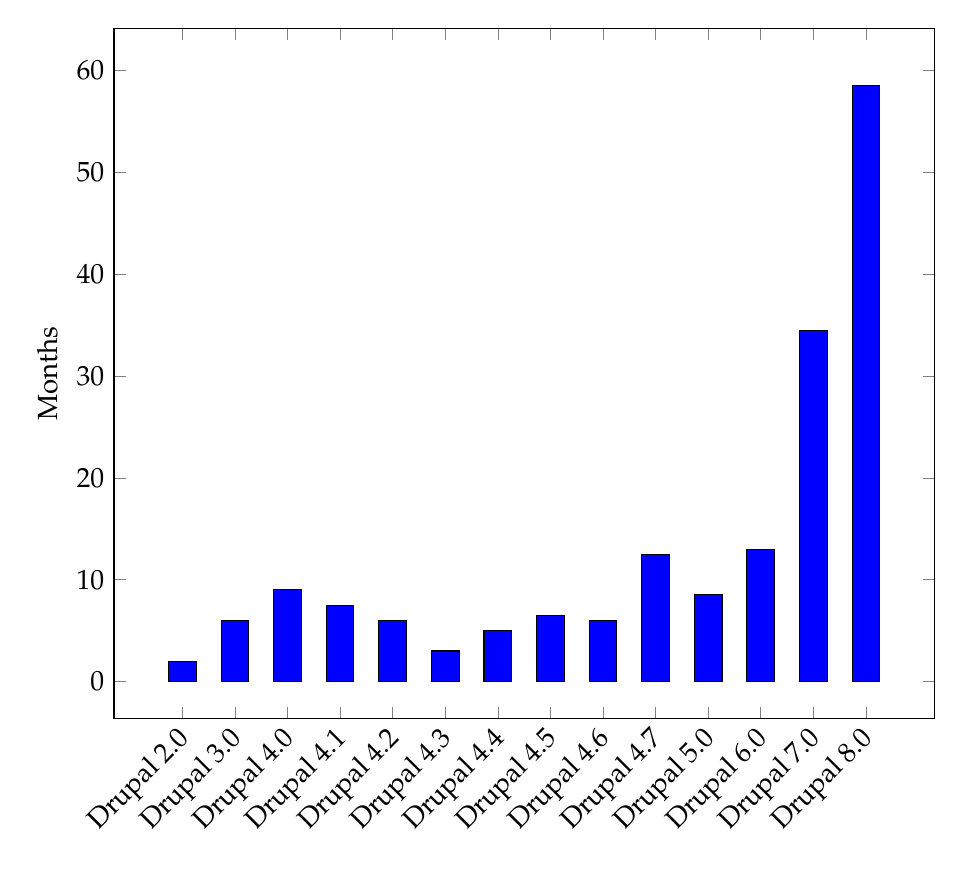
\begin{tikzpicture}
\begin{axis}[width=12cm,
    symbolic x coords={Drupal 2.0, Drupal 3.0, Drupal 4.0, Drupal 4.1, Drupal 4.2, Drupal 4.3, Drupal 4.4, Drupal 4.5, Drupal 4.6, Drupal 4.7, Drupal 5.0, Drupal 6.0, Drupal 7.0, Drupal 8.0},
    xtick=data,
    x tick label style={rotate=45, anchor=east, align=center, yshift=-5pt},
   % label style={font=\tiny},
    ylabel= Months]
    \addplot[ybar,fill=blue] coordinates {
(Drupal 2.0,2) (Drupal 3.0,6) (Drupal 4.0, 9)(Drupal 4.1,7.5) (Drupal 4.2,6) (Drupal 4.3,3) (Drupal 4.4,5) (Drupal 4.5,6.5) (Drupal 4.6,6) (Drupal 4.7,12.5) (Drupal 5.0,8.5) (Drupal 6.0,13) (Drupal 7.0,34.5) (Drupal 8.0,58.5)
    };
\end{axis}
\end{tikzpicture}
	\caption[Total amount of months between major releases]%
	{Number of months between major releases (see footnote \ref{numbering-conventions} to clarify the differences in the numbering conventions). Based on data collected by \textcite{zoubi-history:2016:Online}, under a CC BY-SA 2.0 license.}
	\label{stats-drupal-release}
\end{figure}

It is within this period that this study was carried out, hence, the main events and development that took place in this time will be extensively presented and analysed throughout this thesis. Nevertheless, some of the aspects that characterised this period should be introduced to provide a general overview of the key moments in the history of Drupal and its community. 

In addition to the continued growth in the adoption of Drupal and participation in the project, this period was characterised by a significant change in the organisational processes surrounding the development of version 8 of Drupal core. Figure \ref{drupal-8-core-release} provides an overview of the release cycle of Drupal applied for Drupal 8 \parencite{drupal-core-release-cycle:2014:Online} depicting, for example, clearer stages with regard to the scope of possible technical changes to be included. These stages were defined with the aim of improving coordination and synchronisation to solve dependencies during development. For instance, once the project entered a ``freezing" stage, new features could not be added. Another example of these changes towards a more structured set of processes was the introduction of the notion of ``Core Initiatives"\footnote{Core Initiatives, as well as other relevant organisational changes in the development of core, are extensively discussed and analysed in chapter \ref{chapter:core-system}.} \parencite{drupal-core-initiatives:Online}. The development was divided into several initiatives which were led either by a well-known developer in the community \parencite{drupal-core-initiatives:Online} appointed by Dries or by emergent groups whose proposals were required to fulfil a set of quality control criteria. These initiatives were considered high priority tasks by the community, and included for instance a new theme engine, the inclusion of multilingual capabilities that removed the need for \textit{contributed} modules, and the implementation of web services to allow Drupal to interoperate easily with other systems.

\begin{figure}[H]
	\centering
	\includegraphics[scale=0.8]{img/d8_release_cycle.png}
	\caption[Drupal 8 core release cycle]%
	{Drupal 8 core release cycle. Retrieved \nth{22} September 2014, from \url{https://drupal.org/files/d8_release_cycle.pdf}, under a CC BY-SA 2.0 license.}
	\label{drupal-8-core-release}
\end{figure}

Another key aspect to be highlighted during this period were the substantial technical changes carried out in the architecture, as well as the tensions created in the community as a consequence. The most prominent discussion was focussed on the inclusion of some components of the web application framework Symfony\footnote{Symfony is a FLOSS web application framework based on PHP \parencite{symfony:2017:Online}. It is characterised by a high degree of re-usability and modularity, drawing on other PHP FLOSS components. When compared with Drupal, Symfony's scope is of a lower level of abstraction. For example, it provides more control to the developer, but it requires more effort in writing customised code.} into Drupal's core, which originated in one of the Core Initiatives \parencite{drupal-8-symfony-webservices:2017:Online, drupal-8-symfony-webservices2:2017:Online}. This was also seen as an opportunity to change other major architectural aspects. For example, with regard to the way Drupalistas can interact with the core of the system, since it provided a way to deprecate\footnote{\label{deprecate}In software engineering, deprecated functions or features refers to those that are in the process of being replaced by newer ones \parencite{deprecate:2017:Online}.} the ``hooks system\footnote{As previously discussed in section \ref{sec:what-is-drupal}, hooks are the main means by which modules interact with Drupal core up to version 7 \parencite{drupal-hooks:2016:Online}.}".

Furthermore, these architectural changes did not only have technical consequences, but they could also have potential social ones, since they could affect the nature of the community and the participation in the project. On one hand, the benefits for the community of this new approach were argued for \parencite{drupal-symfony-announcement:Online} on the basis of what was known as the need to ``get off the island" \parencite{getting-off-island:2017:Online}: by following a paradigm similar to that of other PHP frameworks this could attract new PHP developers into Drupal, since it signified the end of a very specific Drupal paradigm which was in part causing the previously discussed ``hard learning curve". On the other hand, other Drupalistas argued that this could cause a ``loss of the hobbysts" in Drupal 8. From the point of view of these Drupalistas, this could produce a loss of the ``hacky" spirit which was the essence of Drupal's technical philosophy. They argued that this ``hacky" spirit embedded in the technology was one of the main reasons why amateurs had been able to experiment and customise Drupal's code easily, and it would especially affect them. In addition, they based their argument on the increment in the shaping of Drupal's architecture towards targeting larger projects, typically carried out by large corporations and the possible interest they may have in changing the project's technical direction \parencite{Rogers2014, kein-debate-1:2014:Online, kein-debate-2:2014:Online}. 

In the end Symfony was included and the ``hooks system" was deprecated\footnote{See previous foonote \ref{deprecate}.}, but the tension surrounding these important and significant technical changes would cause the creation of the first fork of Drupal by a group of Drupalistas: Backdrop\footnote{The main website of the project can be found at \url{https://backdropcms.org}.}. Their intention was announced on 21st August 2013 \parencite{drupal-backdrop:Online}, and they argued in favour of forking on the basis that Backdrop would help to maintain the amateur audience, since the new version of Drupal was oriented to the professional market. The relationships between the Drupal and Backdrop projects were and remain amicable. For example, it is common to find Backdrop developers at Drupal events to present and discuss the project. Nevertheless, the issue remains controversial at times, due to the fear of causing a division in the community. Despite the fork, Drupal 8 was finally released on \nth{19} November 2015 \parencite{d8-release:Online} after five years of development.

\section{The growth of the community}
\label{sec:growth-community}

As previously discussed, the significant growth experienced by the Drupal community is fundamental to contextualise this case study. Considering its size --- more than 1.3 million people registered on Drupal.org --- , the Drupal community cannot be understood as a representative example of either CBPP or FLOSS communities, since most of these communities are of a smaller scale in terms of participants, as it was discussed in chapter \ref{chapter:introduction}. For instance, drawing on the data of Ohloh.net\footnote{See section \ref{subsec:floss-tools}.}, \textcite{oss-size:2017:Online} estimated that 87\% of FLOSS projects have five or fewer committers per year, with only a 0.1\% of them having 200 or more. Thus, this case study should be understood as extreme: a case of a large and global Commons-Based Peer Production community, for which the study of how its self-organisational processes emerged, evolved and scaled up over time, will help to improve our understanding of the phenomenon of Commons-Based Peer Production. The focus in this study will be placed on the effects of this growth on the self-organisational processes of the community rather than on the reasons why this growth occurred, an aspect which would require an in-depth study in itself, and hence was concluded to be out of the scope of this thesis. To this end, this section is devoted to providing a more detailed discussion of the growth experienced by the Drupal community, by presenting and analysing some indicators of this growth in online and offline medium\footnote{Indeed, the online\slash offline distinction within this case study is blurred, and it should be understood as non-binary. These aspects are widely explored in chapter \ref{chapter:methods}, in which the sampling strategy is defined according to a spectrum comprised of ``mostly-online" and ``mostly-offline" contribution activities, on the basis of the medium in which the majority of actions and operations occurred. Nevertheless, in this chapter they are presented as online and offline for simplification purposes.}. The inclusion and comparison in this study of offline activities with equal relevance as online is another novel aspect of this research, since literature on FLOSS has tended to focus on online activities\footnote{These aspects will be explored more extensively in chapter \ref{identifyng-contribution:chapter}, where it is argued that this also relates to the need to broaden our understanding of contribution activities beyond those whose main focus of action is directed towards the digital commons themselves (e.g. writing code or documentation).}.

Regarding online activity, the Drupal community has been undergoing a process of significant growth throughout its existence. This is illustrated by various indicators, such as the increase in the number of users registered at Drupal.org and their increased participation in online activities.

With regard to the number of contributors, a simple indicator of this growth is the surpassing of the million mark of registered users in the main collaboration platform in October 2013 \parencite{drupalorg-1-million:2016:Online}. It is important to notice that this does not imply that all of these Drupalistas will become active contributors, or active in a similar way. As found in many other CBPP communities, an unequal distribution in the degree of participation is regularly found in CBPP. For instance, as found by \textcite{p2pvalue-del12:Online} in their quantitative study of more than 300 cases of CBPP, there is a tendency towards a 90-9-1 distribution power law with regard to participation: 90\% of the participants have a low level of engagement, around 9\% make minor contributions and around 1\% are very active contributors. Hence, as expected from a distribution with these characteristics, the total growth of the community\footnote{The methodological approach followed in this study, based on qualitative methods as will be discussed in chapter \ref{chapter:methods}, makes it difficult to offer a solid argument in terms of generalisation of whether Drupal does or does not follow a 90/9/1 distribution of participation. Nevertheless, the data reported by the community for online activities, as well as the observations carried out by the researcher or the qualitative interviews for offline activities --- whose indicators are less precise ---  were in line with this usual type of distribution with regard to the level of participation found in CBPP communities.} also encompasses a growth in the number of contributors which fall within these different levels of participation. For example, figure \ref{core-committers-release} depicts the number of Drupalistas who carried out at least one commit in Drupal core at the time of each major release, showing, for example, how the number of committers to core in Drupal 8 was more than three times the number of committers in Drupal 7 \parencite{drupal-cores:2016:Online, drupal7-core:2016:Online}.

% Plot for log10 core committers per release
\begin{figure}[H]
\centering
 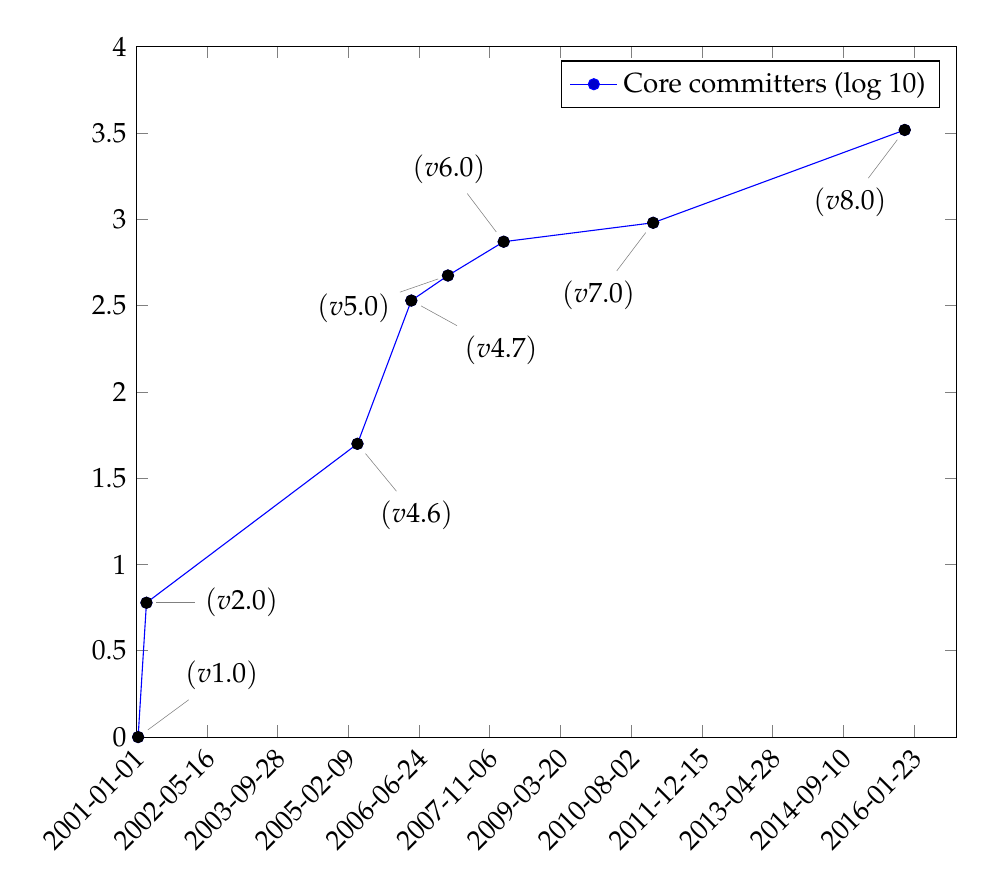
\begin{tikzpicture}
  \begin{axis}[width=12cm, date coordinates in=x,date ZERO=2001-01-01,
               xticklabel=\year-\month-\day,ymin=0,ymax=4,
               x tick label style={rotate=45, anchor=east, align=center, yshift=-5pt},
               label style={font=\tiny},
       xmin=2001-01-01,
       xmax=2016-11-19]
   \addplot coordinates {
(2001-01-15,0)
(2001-03-15,0.7781512504)
(2005-04-15,1.698970004)
(2006-05-01,2.5289167)
(2007-01-15,2.673941999)
(2008-02-13,2.869818208)
(2011-01-05,2.979548375)
(2015-11-19,3.517195898)
   };

\addplot[mark=*] coordinates {(2001-01-15,0)} node[pin=45:{$(v1.0)$}]{} ;
\addplot[mark=*] coordinates {(2001-03-15,0.7781512504)} node[pin=0:{$(v2.0)$}]{} ;
\addplot[mark=*] coordinates {(2005-04-15,1.698970004)} node[pin=-75:{$(v4.6)$}]{} ;
\addplot[mark=*] coordinates {(2006-05-01,2.5289167)} node[pin=-30:{$(v4.7)$}]{} ;
\addplot[mark=*] coordinates {(2007-01-15,2.673941999)} node[pin=-170:{$(v5.0)$}]{} ;
\addplot[mark=*] coordinates {(2008-02-13,2.869818208)} node[pin=100:{$(v6.0)$}]{} ;
\addplot[mark=*] coordinates {(2011-01-05,2.979548375)} node[pin=-100:{$(v7.0)$}]{} ;
\addplot[mark=*] coordinates {(2015-11-19,3.517195898)} node[pin=-100:{$(v8.0)$}]{} ;
\legend{Core committers (log 10)}
\end{axis}
\end{tikzpicture}
	\caption[Number of core committers per release]%
    {Number of core committers (log 10) per release. Based on data collected by \textcite{zoubi-history:2016:Online}. The statistics from Drupal 3.0 to 4.5 could not be found, and they have been omitted. Retrieved \nth{10} March 2016, from \url{http://websolutions.hr/drupal-history}, under a CC BY-SA 2.0 license.}
	\label{core-committers-release}
\end{figure}

A similar sustained growth can be found with respect to the production of \textit{contributed} projects. Figure \ref{contrib-modules-release} depicts the emergence of this pool over several releases, illustrating this growth\footnote{This data might not be completely accurate. In this case, the source of the data is \textcite{zoubi-history:2016:Online}, who estimated it using the closest existing captures from web.archive.org for each release (e.g. \url{http://web.archive.org/web/20041205054156/http://cvs.drupal.org/viewcvs/drupal/contributions/modules/}). In addition, it is also important to remark that unfortunately the number of Drupalistas with permissions to commit over time could not be recovered. Nevertheless, as in the previous cases, the use of figures is intended to illustrate the clear growth of the community, rather than to carry out a detailed analysis which a more quantitative approach would require.}.

% Plot for log10 contributed modules per release
\begin{figure}[H]
\centering
 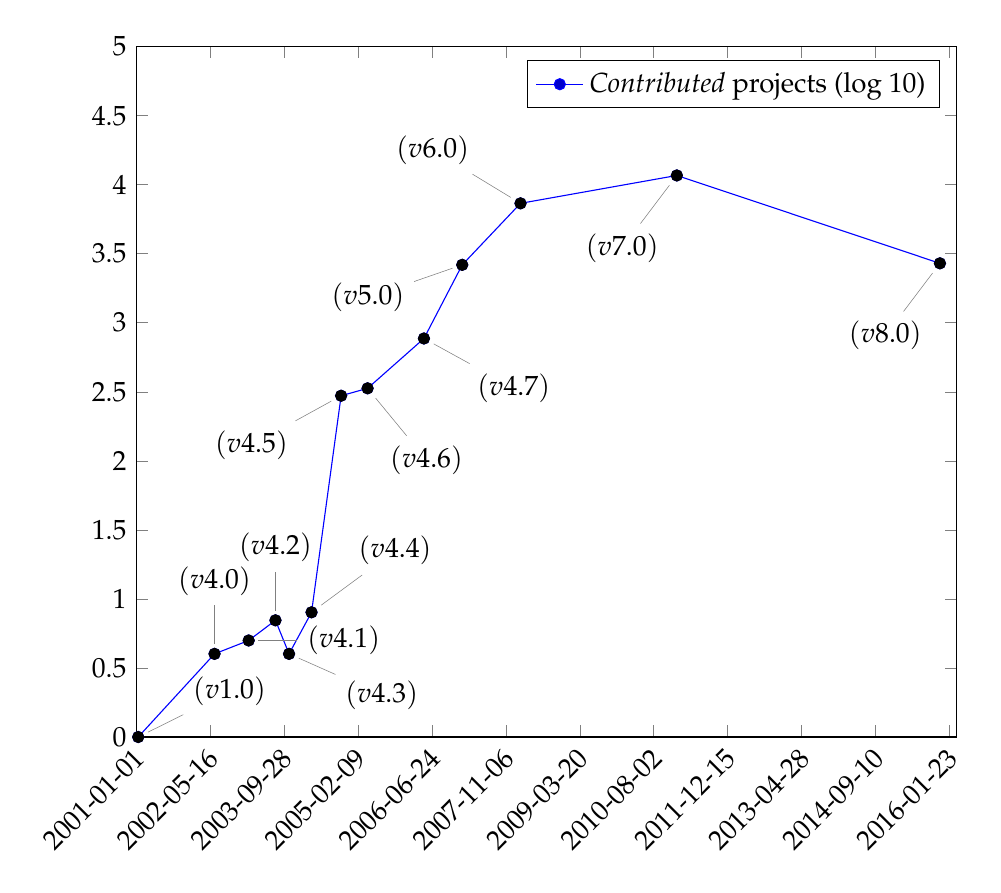
\begin{tikzpicture}
  \begin{axis}[width=12cm, date coordinates in=x,date ZERO=2001-01-01,
               xticklabel=\year-\month-\day,ymin=0,ymax=5,
               x tick label style={rotate=45, anchor=east, align=center, yshift=-5pt},
               label style={font=\tiny},
       xmin=2001-01-01,
       xmax=2016-03-10]
   \addplot coordinates {
(2001-01-15,0)
(2002-06-15,0.6020599913)
(2003-02-01,0.6989700043)
(2003-08-01,0.84509804)
(2003-11-01,0.6020599913)
(2004-04-01,0.903089987)
(2004-10-18,2.471291711)
(2005-04-15,2.525044807)
(2006-05-01,2.88592634)
(2007-01-15,3.419294722)
(2008-02-13,3.864629725)
(2011-01-05,4.066586796)
(2015-11-19,3.430236353)
   };
   
\addplot[mark=*] coordinates {(2001-01-15,0)} node[pin=25:{$(v1.0)$}]{} ;
\addplot[mark=*] coordinates {(2002-06-15,0.6020599913)} node[pin=-270:{$(v4.0)$}]{} ;
\addplot[mark=*] coordinates {(2003-02-01,0.6989700043)} node[pin=0:{$(v4.1)$}]{} ;
\addplot[mark=*] coordinates {(2003-08-01,0.84509804)} node[pin=-270:{$(v4.2)$}]{} ;
\addplot[mark=*] coordinates {(2003-11-01,0.6020599913)} node[pin=-20:{$(v4.3)$}]{} ;
\addplot[mark=*] coordinates {(2004-04-01,0.903089987)} node[pin=45:{$(v4.4)$}]{} ;
\addplot[mark=*] coordinates {(2004-10-18,2.471291711)} node[pin=-150:{$(v4.5)$}]{} ;
\addplot[mark=*] coordinates {(2005-04-15,2.525044807)} node[pin=-75:{$(v4.6)$}]{} ;
\addplot[mark=*] coordinates {(2006-05-01,2.88592634)} node[pin=-30:{$(v4.7)$}]{} ;
\addplot[mark=*] coordinates {(2007-01-15,3.419294722)} node[pin=-170:{$(v5.0)$}]{} ;
\addplot[mark=*] coordinates {(2008-02-13,3.864629725)} node[pin=145:{$(v6.0)$}]{} ;
\addplot[mark=*] coordinates {(2011-01-05,4.066586796)} node[pin=-100:{$(v7.0)$}]{} ;
\addplot[mark=*] coordinates {(2015-11-19,3.430236353)} node[pin=-100:{$(v8.0)$}]{} ;   
   
\legend{\textit{Contributed} projects (log 10)}
\end{axis}
\end{tikzpicture}
	\caption[Number of \textit{contributed} projects per release]%
    {Number of \textit{contributed} projects (log 10) per release. Based on data collected by \textcite{zoubi-history:2016:Online}, drawing on captures from web.archive.org. The statistics from Drupal 2.0 and 3.0 could not be found, and they have been omitted. Retrieved \nth{10} March 2016, from \url{http://websolutions.hr/drupal-history}, under a CC BY-SA 2.0 license.}
	\label{contrib-modules-release}
\end{figure}

The figure depicts constant growth, with the exception of the difference between Drupal 8 with respect to Drupal 7. This difference can be explained, however, by the time at which the data for Drupal 8 was collected, and the large difference in the period to develop modules between major releases. Contributed projects typically start to be developed and ported once the final release has been made, or some months before. Hence, the numbers refer to a period of approximately thirteen months since the release. A similar reason can explain the lower amount of contributed modules for Drupal 4.3 with respect to 4.2, since the difference between releases was three months (see figure \ref{stats-drupal-release}).

In a similar way as in the case of online activities, the Drupal community has experienced a significant growth in the organisation of offline activities and participation in them. The first international F2F meeting in Belgium in 2005\footnote{See section \ref{subsec:offline-side}.} would be a source of inspiration for the emergence and spread of a wide range of different types of F2F events, ranging from local events focussed on presentations, sprints to contribute back to the community or simply informal meetings for drinks with other Drupalistas, to events whose organisational dynamics more closely resemble those of conferences. For example, \textit{DrupalCons} (see figure \ref{drupalcon-amsterdam-2014}): major international Drupal events which take place over the course of a week. They include peer-reviewed presentations, more informal presentations or ``BoFs" (Birds of a Feather), community summits, code sprints, social events and public Drupal Association meetings, to name but a few activities. They are organised by the Drupal Association\footnote{The organisational changes experienced over time will be extensively discussed in chapter \ref{mostly-offline-cons:chapter}.}, with the support of the local community of the city in which it is held. They are commonly organised on a yearly basis at a continental level: originally in North America and Europe, although more recently there were first editions in Australia (2013) \parencite{drupalcon-aus:2016:Online}, South America (2015) \parencite{drupalcon-sa:2016:Online}, and Asia (2015) \parencite{drupalcon-asia:2016:Online}. Attendance fees are significantly costly, around the hundreds of euros\slash dollars. For instance, the price of a regular ticket for the whole event at \textit{DrupalCon} Amsterdam 2014 was 500\euro{}.


\begin{figure}[H]
	\centering
	\includegraphics[scale=0.32]{img/events/drupalcon_human_drop.jpg}
	\caption[\textit{DrupalCon} Amsterdam 2014]%
    {Group picture at \textit{DrupalCon} Amsterdam 2014, which attracted more than 2,000 participants. The group is forming a ``human drop" resembling Druplicon, the logo of Drupal (see figure \ref{druplicon}). Retrieved \nth{13} November 2014, from \url{http://chapterthree.com/blog/chapter-three-drupalcon-amsterdam}.}
	\label{drupalcon-amsterdam-2014}
\end{figure}

The growth of offline participation can be observed using indicators such as attendance to these \textit{DrupalCons}. For example, figure \ref{dcons-eu-na} depicts the overall growth in the number of attendees in Drupalcons held in Europe\footnote{The data from the two events in 2005 might not be as accurate as the rest. It is indicated as \textless 50 and approximately 100. Hence, those estimated figures (50 and 100) have been employed for the coordinates chart, and combined within the same year in the graph but depicted by a line. It is also important to notice that the first \textit{DrupalCon} event in Europe was organised in 2007. The previous events were part of major FLOSS conferences, such as FOSDEM. In any case, the figures are useful to provide an overview of the growth, since they refer specifically to attendance of Drupalistas.} and North America\footnote{The data from 2005, 2006 and 2007 may not be as accurate as the rest. It is indicated as \textgreater 100, approximately 150 and \textgreater 300 respectively. Hence, those estimated figures (100, 150 and 300) have been employed for the chart.  It is also important to notice that, according to the documentary analysis  \parencite{drupalcon-vancouver:2016:Online}, the first specific \textit{DrupalCon} event in North America was organised in 2006 in Vancouver.  Nevertheless, experienced Drupalistas who were interviewed explained that the \textit{DrupalCon} in Boston (2008) should be considered the closest to what is now considered a \textit{DrupalCon}. Previous events (including 2007) were part of major FLOSS conferences, such as OSCOM (Open Source Convention). In any case, the figures are useful to provide an overview of the growth, since they refer specifically to attendance of Drupalistas.}.



%Plot combining attendance to DrupalCon Europe and DrupalCon America
\begin{figure}[H]
\centering
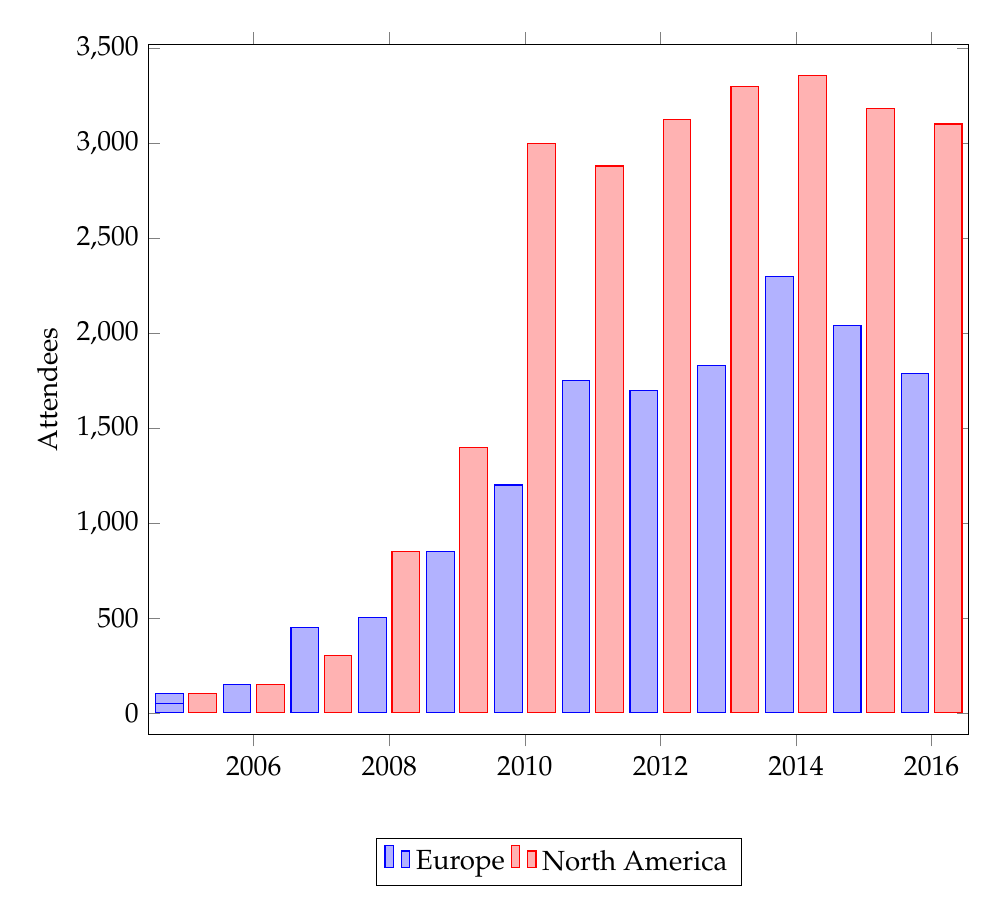
\begin{tikzpicture}
\begin{axis}[
	x tick label style={
		/pgf/number format/1000 sep=},
	ylabel=Attendees,
	enlargelimits=0.05,
	legend style={at={(0.5,-0.15)},
	anchor=north,legend columns=-1},
	ybar,
]
\addplot 
	coordinates {(2005,50)(2005,100) (2006,150) (2007,450) (2008,500) (2009,850) (2010,1200) (2011,1751) (2012,1700) (2013,1830) (2014,2300) (2015,2039) (2016,1787)};
\addplot 
	coordinates {(2005,100) (2006,150) (2007,300) (2008,850) (2009,1400) (2010,3000) (2011,2881) (2012,3127) (2013,3300) (2014,3357) (2015,3186) (2016,3102)};
\legend{Europe,North America}
\end{axis}
\end{tikzpicture}
\caption[Number of attendees to \textit{DrupalCon} events in Europe and North America]%
    {Number of attendees to \textit{DrupalCon} events in Europe and North America. Based on data reported by the \textcite{drupal-association-dcons-attendance:2016:Online}.}
	\label{dcons-eu-na}
\end{figure}

The growth in the participation of Drupalistas in \textit{DrupalCons} was particularly significant in the periods 2008-2011 for the case of Europe and 2008-2010 for the case of North America. As it will be discussed in section \ref{subsec:dcons-growth}, this was a clear point of change with regard to the organisational processes of \textit{DrupalCons}. There were slight decreases with respect to the previous edition in 2011 for the case of North America, and in 2012 for the case of Europe. However, after those editions growth continued. Nevertheless, the most recent editions (2015 and 2016) depict a more prominent decline in attendance. This has awoken concern in the community, and it is commonly explained by Drupalistas as a loss of momentum in adopting Drupal due to the long time (five years) which it had taken to develop Drupal 8 \parencite{drupal-momentum:2016:Online}, in a similar way as the previous decline after Drupal 7\footnote{An in-depth analysis of this aspect was beyond the scope of this study. Other hypothesis could be based on a reduction in the rate of growth, as in the case of Wikipedia \parencite{suh2009singularity}, or the impact of the fork described in section \ref{subsec:d7-d8}.}.

Other indicators of this growth can be found in the growing numbers of \textit{DrupalCamps}\footnote{\label{fn-dev-days}In addition to \textit{DrupalCamps}, events specialised in specific roles, a topic that will be more extensively discussed in section \ref{par:roles},  such as Drupal Dev Days --- aimed at backend developers --- or Frontend United --- aimed at themers --- are also held by the community. While they were distinctively considered during certain stages of this study --- for example while studying the notion of contribution in chapter \ref{identifyng-contribution:chapter} --- they are included as part of this category in this classification for simplification purposes because of their similarities in organisational dynamics.} (see figure \ref{drupalcamp-spain-2014}): for example, while in 2007 six \textit{DrupalCamps} were organised, the number ascended to 67 in 2013 \parencite{ostraining-list-drupalcamps:2016:Online}. These are two or three day events focussing on sharing knowledge within the community. They include peer-reviewed  presentations, Drupal sprints and social events. They are frequently organised once a year, typically at a national level. However, in large countries or those countries with the largest Drupal communities they are organised regionally. For example, in the case of the UK there are events such as \textit{DrupalCamp} London, \textit{DrupalCamp} North West, \textit{DrupalCamp} North East, \textit{DrupalCamp} Brighton and \textit{DrupalCamp} Bristol. They are organised by local communities, and their attendance requires a relatively low fee which depends on the country (e.g. for the UK around 30-40\pounds). Their levels of attendance vary, but it is commonly around the hundreds. For example, events which have been held for consecutive years tend to attract around 200-300 people.

\begin{figure}[H]
	\centering
	\includegraphics[scale=0.37]{img/events/drupalcamp_spain.jpg}
	\caption[\textit{DrupalCamp} Spain 2014]%
    {Group picture at \textit{DrupalCamp} Spain 2014 (May). Retrieved \nth{9} July 2014, from \url{http://2014.drupalcamp.es}.}
	\label{drupalcamp-spain-2014}
\end{figure}

Similar indicators of this growth can be found in the case of local events\footnote{An exhaustive list of all these events over time does not exist, to the best of my knowledge. The most precise source found is \url{https://groups.drupal.org/events}. It operates as a wiki in which Drupalistas add some of the events. The collected data is employed by other sites, as in the case of the presented World map visualisation by \textcite{drupical:2016:Online}. However, it is important to notice that this list may not be completely accurate. For example, one of the smaller local events which I attended, organised via Meetup.com, was not included within this data. In addition, external sources such as \textcite{ostraining-list-drupalcamps:2016:Online} were employed, since they provide a historical archive. However, they are also limited. For example, in the event referred to the collection of data stopped in 2013.}, or the nearly 600 regional groups listed at Drupal.org \parencite{drupalorg-groups:2016:Online}. For instance, tens of local Drupal meetups are held every month worldwide: a filtered list of local events in Drupical \parencite{drupical:2016:Online} displays 38 events (see figure \ref{drupical-local-events}) being organised in a month's time. 

\begin{figure}[H]
	\centering
	\includegraphics[scale=0.25]{img/offline/drupical_march_2017}
	\caption[World map of Drupal local events]%
    {Forthcoming Drupal local events in a month's time at the time of writing (01/03/2017). Screenshot from Drupical.com. Retrieved \nth{01} March 2017, from \url{http://www.drupical.com}.}
	\label{drupical-local-events}
\end{figure}

The characteristics and functions of these local events differ significantly in their purpose and level of formality: from the most informal and social events (Drupal Beer and Chat), to those focussed on presentations on case studies or the technical advances of the platform for learning purposes (Drupal Show and Tell). For example, the following local events were studied as part of this research:

\textbf{Drupal Beer and Chat\footnote{The names given by Drupalistas to all these events differ in different local communities. For example, in Spanish local communities similar events are commonly known as ``Drupaladas".}}

These are considerably informal events in which people with an interest in Drupal meet in a pub to discuss Drupal, without an agenda. In the case of the observation in London, they commonly started around 7pm, and finished once the pub was closed, typically 11pm to 12am. They attracted tens of people --- an average of 15 to 20 during observations --- and were mainly organised via Meetup.com\footnote{\url{http://www.meetup.com/London-Drupal-Pub-Meet/}, accessed on \nth{14} November 2014.}. They were organised approximately once a month.

\textbf{Drupal Show and Tell}

These are informal presentations about diverse topics in Drupal, such as case studies, presenting new technologies and modules, and sessions to advise on the implementation of certain functionalities (see figure \ref{drupal-show-tell}). In the case of the observations carried out in London, they typically started at 6pm, and concluded within 1.5 or 2 hours. They were held in rooms which enabled the use of slides (e.g. universities and company meeting rooms). After the event, there was commonly a more informal meeting, whose dynamics were similar to those of a Drupal Beer and Chat. They also attracted tens of people --- typically between 25 to 35 --- and were similarly organised via Meetup.com\footnote{\url{http://www.meetup.com/drupal-show-and-tell/}, accessed on \nth{14} November 2014.}  and mailing lists. They were organised approximately once a month.

\begin{figure}[H]
	\centering
	\includegraphics[scale=0.09]{img/offline/drupal_show_tell_london.jpg}
	\caption[London Drupal Show and Tell]%
    {Picture from a London Drupal Show and Tell in January 2016. Retrieved \nth{17} January 2016, from \url{https://www.meetup.com/drupal-show-and-tell/photos/26670134/445910901/}. Chandeep Khosa.}
	\label{drupal-show-tell}
\end{figure}

\textbf{Drupal Sprint}

These are events focussed on contributing back to the Drupal community, with organisational dynamics similar to those of ``hackathons" \parencite{lapp20072006}. Their participants collaborate to write software, documentation or carry out testing, among other activities (see figure \ref{drupal-sprint-weekend}). Additionally, there are sometimes Drupal training sessions to help newcomers to start contributing (Drupal Ladders\footnote{\url{http://drupalladder.org/}, accessed on \nth{14} November 2014.}). In the case of London, these events typically took place throughout whole weekends, starting at around 10am and finishing around 6pm. They were held in ``open spaces" rooms, where participants could bring their laptops and sit next to each other to collaborate. During observation, they attracted around 10-20 people. They were mainly organised via EventBrite\footnote{\url{http://www.eventbrite.co.uk/o/drupal-london-community-61878136}, accessed on \nth{14} November 2014.}, but also promoted via Drupal.org. They were organised once a month approximately.

\begin{figure}[H]
	\centering
	\includegraphics[scale=0.55]{img/events/drupal_coding_sprint.jpg}
	\caption[Drupal Sprint Weekend]%
    {Picture from a Drupal Sprint Weekend, to promote a new event in April 2014. Retrieved \nth{27} August 2014, from \url{https://groups.drupal.org/node/416908}, under a CC BY-SA 2.0 license.}
	\label{drupal-sprint-weekend}
\end{figure}

\textbf{Drupal Coworking Day}

These are informal events where Drupal professionals, typically freelancers, but also people working for companies, meet to work together or ``coworking" \parencite{spinuzzi2012working} and help each other with their personal or professional Drupal projects. For instance, in observations in London these events took place during workdays, starting at around 10am and finishing at around 5pm. Although, as with the events previously described, there was no cost for attendance, in this case they required a RSVP due to limits in the number of places --- ten for this specific case. They were mainly organised via Meetup.com\footnote{\url{http://www.meetup.com/London-Drupal-Coworking-Meetup}, accessed on \nth{14} November 2014.}, and held approximately twice a month.

Overall, the previous indicators illustrate the significant growth experienced by the community over time, while the concrete examples illustrate its diversity. In the next section another relevant aspect is discussed, that of ``do-ocracy" in relation to the culture of the community.

\section{Life in a ``do-ocracy": a model of governance?}
\label{sec:do-ocracy}

When asked about the model of governance of the Drupal project, Drupalistas commonly defined it as a ``do-ocracy". ``Do-ocracy" is a notion that encourages open participation. It is based on the self-allocation of tasks, and it allows those who carry out these tasks to be recognised and become more influential in order to make decisions when ``rough consensus" \parencite{russell2006rough} is necessary to be reached. The following excerpt from Dries \parencite[514]{bacon2012art}, the original creator of Drupal, illustrates how these main characteristics of ``do-ocracy" shape the day-to-day life of the Drupal community:

\begin{quotation}
``[...] The Drupal community uses a ``do-ocracy" model, meaning people work on what they want to work on, instead of being told what to work on. Decisions are usually made through consensus building and based on technical merit, trust and respect."
\end{quotation}

Not surprisingly, the notion of ``do-ocracy" presents characteristics that resemble those of the hacker culture discussed in section \ref{subsec:hacker}. For example, in relying on meritocratic values --- such as the ``technical merit" mentioned in the quote above --- and encouraging the focus to be placed on contribution activities and quality, rather than on the personal characteristics of those who carry them out --- ``Hackers should be judged by their hacking, not criteria such as degrees, age, race, sex, or position" \parencite[35]{levy1984hackers}. Another example is the mistrust of formal authority, as part of a more general anti-bureaucratic attitude of hackers. A ``do-ocracy" operates on the idea that those who mobilise more resources towards a certain task and demonstrate their merit to the community have the legitimacy to make decisions that relate to that task, rather than legitimacy being based on arbitrary rules that consolidate power representing a threat for their creative impulses \parencite[25]{levy1984hackers}.

The notion of ``do-ocracy" is commonly found to describe the governance of organisational processes of CBPP communities \parencite[e.g.][]{mateos2008institutions, fuster2010governance, zacchiroli2011debian, kostakis2014production}. For example, \textcite[282]{fuster2010governance} incorporated this notion in the context of the study of the governance of online creation communities and defined it as follows:

\begin{quotation}
``[...] Doocracy refers to the idea that there is no external body or hierarchy that decides how actions should be carried out. In other words, in a doocracy authority over an action is held directly by those developing it. Furthermore, participants gain influence and authority in the process according to their merits and the resources for `doing' that they mobilize (such as time or attention)."
\end{quotation}

In addition, these ``do-ocratic" characteristics incorporate numerous similarities with those presented in the literature review of governance of CBPP communities in section \ref{subsec:governance-cbpp}, such as the attributes defined by \textcite{benkler2006commons}. The previous quote by Dries depicts, for example, the self-assignation of tasks, whose outcomes' quality is scrutinised through peer-reviewing processes carried out by the community.

Nevertheless, these ``do-ocratic" characteristics also imply an inherently blurred and informal nature, which can become a source of inner contradictions and tensions as communities adapt their self-organisational processes over time. For instance, the willingness to decentralise the governance of the community may produce tensions with respect to the rejection of bureaucratisation, since formal rules may be interpreted as arbitrary with the aim of consolidating power in the hackers' eyes.

In the case of the Drupal community similar tensions and inner contradictions emerged, for example, when the community grew and discussed the necessity to formalise the self-organisational processes to scale up. For instance, the following excerpt, from a post by Dries \parencite{do-ocracy01:2016:Online} in the context of a discussion about Drupal governance in March 2013, depicts some of these tensions and frustrations generated by a lack of clarity in certain processes, in this case those related to the governance of the main collaboration platform and the Drupal Association:

\begin{figure}[H]
  \centering
\includegraphics[scale=0.5]{img/quotes_replacement/do-ocracy-dries.png}
\caption[Excerpt from the article ``Creating a structure for Drupal governance"]{Excerpt from the article ``Creating a structure for Drupal governance". Retrieved \nth{27} July 2017, from \url{http://buytaert.net/creating-a-structure-for-drupal-governance}.}
\label{do-ocracy-dries}
\end{figure}

Hence, when applied to the model of governance of large and global CBPP communities, the notion of ``do-ocracy" lacks relevant aspects, such as the emergence of more formal organisational forms depicted, for example, by the numerous institutions created over time by the Drupal community. For this reason, this study incorporates the notion of ``do-ocracy" not as a model of governance, but as part of a strong culture within the Drupal community \parencite{melanccon2011contributing}, whose values are interrelated and influenced by the values of the hacker culture discussed in section \ref{subsec:hacker}. To this end, the model of governance is a subject matter of this study in itself, in which the influence of the ``do-ocratic" culture is considered as relevant in the shaping of the organisational processes of peer production over time, but assuming that, as shown in the literature review in chapter \ref{chapter:introduction}, there remains a necessity to improve our understanding of how large and global CBPP communities, such as Drupal, organise themselves and scale up while remaining viable over time.

Furthermore, this research conceptualised tensions\footnote{Further details about how the notion of tension is incorporated through the main theoretical framework employed in this study will be presented in chapter \ref{sec:theoretical-frameworks}.}, as those discussed between the anti-bureaucratic attitude and the formalisation of processes to decentralise the governance, as ``windows of opportunity" to follow and collect data during the study. Hence, these tensions will help to 
improve our understanding of the emergence of the processes and structures which the Drupal community has created over time. For example, to improve our understanding of how decentralisation, a key notion to be explored in CBPP as argued in chapter \ref{chapter:introduction}, occurred or whether it did. This study develops from the notion of decentralisation in the context of CBPP of \textcite[62]{benkler2006wealth} as the ``conditions under which the actions of many agents cohere and are effective despite the fact that they do not rely on reducing the number of people whose will counts to direct effective action", applying it to question whether decentralisation occurred in the peer production activities of the community and how it did. This was materialised, for example, by exploring how legitimacy emerged and changed over time in the community in order to decentralise decision-making to perform changes in the digital commons, or to organise events; or to analyse whether practices regarding decision-making related to quality assurance were decentralised and how this occurred.

Another example of opportunity for further study, which arose from the aforementioned tension, is to be found in the need to explore the changes experienced in the organisational processes over time and the organisational dynamics. As stated by \textcite[61]{benkler2006wealth}: ``the salient characteristic of commons, as opposed to property, is that no single person has exclusive control over the use and disposition of any particular resource in the commons. Instead, resources governed by commons may be used or disposed of by anyone among some (more ore less well-defined) number of persons, under rules that may range from `anything goes' to quite crisply articulated formal rules that are effectively enforced". As discussed in chapter \ref{chapter:introduction}, there is a lack, however, of an in-depth understanding of how these ``doocraticly-shaped" rules emerge, operate, are enforced and change over time in large communities, with the few exceptions of largely studied communities such as Wikipedia \parencite{viegas2007hidden, forte2009decentralization}.

This discussion of the notion of ``do-ocracy" concludes the introduction to the case study and the fundamental concepts that surround it in order to frame this research. With the aim of framing the previously discussed gaps in the literature into research questions, the next section presents the main research question and the research sub-questions tackled in this study.

\section{Research questions}
\label{subsubsec:state-art:drupal:case-study}

The main research question tackled in this study is as follows:

\emph{``How does a large and global Commons-Based Peer Production community self-organise?"}

The concepts of ``Commons-Based Peer production community", ``large" and ``global" have been discussed and framed within the context of this case study in chapters \ref{chapter:introduction} and \ref{chapter:case-study}, however, it is important to note that by ``self-organisation" the main research question draws on the efforts to explore the use of this concept within social science. Instead of relying on an undesirable monolithic definition of the concept  \parencite{gilbert2015self, anzola2016self}, this study develops from the notion of self-organisation characterised by four shared features within the literature suggested by \textcite{gilbert2015self}. Firstly, the formation of patterns, which are commonly ``designated by nominalised verbs" \parencite[4]{anzola2016self}. For example, in the case of Commons-Based Peer Production, ``cooperation\footnote{See section \ref{subsec:state-art:cbpp}.}". Secondly, the concept of autonomy, referring to the changes in the self-organisational system originating from the entities of the system or the interactions between them, rather than from a central source of control. For instance, this is depicted in the case of CBPP in the planification and execution of peer-production tasks in a decentralised manner\footnote{See section \ref{subsec:governance-cbpp}.}. Thirdly, referring to the robustness and resilience of self-organised systems, with respect to the ability of these systems to resist and to adapt to change respectively. This case study draws on this feature, for example, by incorporating tensions, as those originated by ``do-ocratic" and hacker culture\footnote{See section \ref{sec:do-ocracy}.}, as ``windows of opportunity" to follow and collect data during the study. Fourthly, dynamics, referring to the variation of the characteristics of self-organisational systems over time. For example, in this case study, carrying out the analysis of the self-organisational processes considering these variations, such as decentralisation of decision-making and formalisation. 

In addition, it is also important to remark that in order to tackle the main research question, a set of research sub-questions are also formulated and addressed in subsequent chapters.

Firstly, an essential element in order to frame the main research question through the study of the self-organisational processes themselves is related to the notion of contribution within FLOSS and CBPP communities. As it was presented in section \ref{subsubsec:state-art:floss:academic-research}, the studies which analyse the relationship between contribution and organisational aspects have typically focussed their attention on the most visible outcome of contribution: the collaboratively built shared objects. For instance, the most well-known type of contribution activity in FLOSS communities is the development of source code and, consequently, this has been typically the most studied. To this end, chapter \ref{identifyng-contribution:chapter} will present the findings regarding the exploration of this notion, helping to shed light on other activities that have not been widely studied due to their lack of visibility. This aspect is especially critical in a community that, as previously discussed, has been characterised as ``code-centric" \parencite{Zilouchian2011, Sims2013, nordinmotivation2014}.  Hence, this enables the identification and consideration throughout the study not only of the activities which are ``officially" understood as contributions, such as those listed in the main collaboration platform, but also of those which have remained less visible. The research sub-question that will be tackled during this chapter is as follows:

\emph{``What types of activities are understood as contributions in the Drupal community and in what ways are these recognised?"}

Secondly, once these contribution activities are identified, the focus of this thesis will shift towards improving our understanding of the main organisational aspects and dynamics that surround the development of these contribution activities. To this end, chapters \ref{sec:custom-to-contrib} to \ref{mostly-offline-cons:chapter} will address the study of the emergence of and changes in these self-organisational processes. The way in which the evolution of these processes responded to general organisational dynamics of formalisation and decentralisation in order to scale them up will then be discussed, as well as how these dynamics affected these processes to different degrees. To this end, the following research sub-questions will be tackled during these chapters:

\begin{itemize}
	 \item \emph{``What are the main organisational aspects and dynamics that have characterised the growth of a global CBPP community of such a scale?"}
	 \item \emph{``What type of governance emerged in the Drupal community?"}
\end{itemize}

Finally, once all these organisational aspects and dynamics have been extensively explored and analysed, the underpinnings to tackle the main research question are laid out. Thus, chapter \ref{multilevel:chapter} will address the main research question, providing a discussion of the central argument around the emergence of \textit{polycentric} governance as the main explanation in order to understand the manner in which the Drupal community has managed to self-organise while remaining viable, while contextualising the argument with respect to previous literature on Commons-Based Peer Production. The fundamental aim will be to offer an explanation of how Drupalistas have been able to organise themselves not just by one, but by multiple governing authorities at different levels varying in the degree of \textit{organicity}.

\section{Conclusion}

Throughout this chapter the fundamental aspects to contextualise the case study for this research were introduced. A brief historical overview of Drupal and its community was provided, illustrating the emergence and growth of a well-known case of Commons-Based Peer Production. This historical account should not be understood as exhaustive, but rather as an overview of the principal aspects necessary to frame this research, such as the increase in users, the emergence of more formal institutions and the tensions experienced as part of the growth of the community.

Among these aspects, two were more extensively discussed on the basis of their relevance for this research. Firstly, the growth experienced in participation in the community through both online and offline media. This aspect is key, since it provides an opportunity to explore organisational dynamics within the context of an extreme case study of Commons-Based Peer Production, hence enabling an improvement in our understanding of how these self-organisational processes emerge, evolve and scale up over time while remaining viable in these conditions. Secondly, the notion of ``do-ocracy" was explored and discussed. It was argued that, despite community accounts, this notion should not be understood as a model of governance since, although it is useful to understand certain characteristics of smaller CBPP communities, the use of the term ``do-ocracy" oversimplifies the complexity hidden behind the governance of the self-organisational processes within the case study. Instead, this study incorporates this notion --- the values  of which were argued to have been inspired by and subsumed within those of hacker culture --- as a relevant force in shaping the self-organisational processes of the Drupal community as well as its governance, but developing from the assumption that these issues require further exploration from a sociological perspective. In addition, the contradictions presented by some of the principles of these cultural forces, such as the tension between calls to formalise certain processes related to decision-making in order to decentralise them, and the common anti-bureaucratic attitude of hackers, were argued to be points of tension, the study of which will help the understanding of the emergence of organisational structures and processes in the community over time. To conclude, the research questions tackled in this study were presented.

With the aim of starting to address these questions, the next chapter will introduce the main theoretical framework employed in order to conceptualise this case study for its exploration: Activity Theory.

%% Chapter with discussion of theoretical framework
\chapter{The exploration of self-organisation via contribution activities: conceptualising Drupal through an Activity Theory lens}
\chaptermark{Activity Theory}
\label{sec:theoretical-frameworks}

This chapter presents an overview of the case study conceptualised through Activity Theory, the main theoretical framework employed for this research. Rather than a theory in the strict sense, Activity Theory is an analytical tool, a lens that helps researchers and practitioners to analyse complex activities, such as in Free\slash Libre Open Source Software as part of the wider phenomenon of Commons-Based Peer Production.

Firstly, a summary of Activity Theory will be presented in section \ref{subsec:at}, providing a historical overview of the three different generations of Activity Theory, the main theoretical concepts underpinning it, its limitations and discussions of activity theorists about it. Secondly, section \ref{subsec:why-at} offers a summary of the reasons why Activity Theory has been chosen for the study of peer production. Finally, section \ref{subsec:at-conceptualisation} provides a detailed explanation of the process carried out to analyse the activities involved in Drupal, drawing on the main concepts of Activity Theory, as well as a set of practical examples of its application to the case study.

\section{A historical overview of Activity Theory}
\label{subsec:at}

\subsection{Historical roots and the first generation}

The historical roots of Activity Theory (AT) can be found in classical German philosophy, from Kant to Hegel, as well as in the work of Marx and Engels. In ``\textit{Theses on Feuerbach}", \textcite[143-45]{marx1845theses} defined the idea of object-oriented activity and discussed the relationship between object and subject during production. According to Marx, the subject produces itself by producing the object while transforming the object's nature. The process is understood as a historical phenomenon, which is dependent on social practices. Another important influence of classical Marxism in AT is the concept of inner contradictions within the system, which can result in a force of development \parencite{hegel1861lectures}.

The main theoretical pillars of AT started being developed in the 1920s, and can be traced within the Soviet cultural-historical psychology field pioneered by Vygotsky, Leont'ev and Luria \parencite{engestrom1999activity}. A key concept is that of mediated action proposed by \textcite{vygotsky1978mind} as an alternative to the behaviourist views on human activities at the time. According to Vygotsky, human action is mediated by culturally meaningful artefacts. By collaborating in the development of activities with other humans, the meanings, social norms and modes of acting are internalised by the individual. This relationship between the subject, the object and the cultural means, norms and signs proposed by Vygotsky, is usually represented as a triangle (see figure \ref{vygotsky-first-gen}), in which the artefacts also embed some of these cultural properties.

\begin{figure}[H]
	\centering
	\includegraphics[scale=0.6]{img/vigotsky_first_gen.png}
	\caption[Vygotsky's model of mediated action]%
	{Vygotsky's model of mediated action: the first generation. \textcite{flavin2012disruptive}.}
	\label{vygotsky-first-gen}
\end{figure}

As in the case of other socio-cultural perspectives \parencite{kaptelinin2012}, this model assumes the social nature of the human mind, as well as its inseparability from the activity. Thus, activities are influenced by the characteristics of the subjects and the objects, and vice versa. For instance, as exemplified by \textcite{kaptelinin2012}, whether a mathematical problem can be solved by a certain subject depends on the characteristics of the object, for example how hard the mathematical problem is. It is also dependent on the characteristics of the subject, for example the subject's mathematical skills. The subject's skills in mathematics are influenced by its previous experience in solving mathematical problems. Hence, while the subject's abilities influence solving the mathematical problem, solving mathematical problems will also influence the subject's abilities over time, for example, improving their knowledge and skills. Therefore, over time, the object and the subject are transformed by the activity, and subjects are also produced by the activities \parencite{kaptelinin2012}.

Subsequently \textcite{leontjev1978activity}, as part of a reaction against the work of Vygotsky, developed the notions of mediated social processes and established the concept of activity as an unit of analysis. This definition of the collective activity system as unit of analysis allowed the connection between psychological, organisational and cultural approaches. Hence, rather than focussing exclusively on the individual as in previous approaches, the interactions between the subject, the artefacts and other individuals under certain organisational settings can be explored. In addition, he distinguished between the concepts of activity, action and operation (see figure \ref{leontiev-three-level-model}) and developed them in a more precise manner:

\begin{itemize}
	\item \textit{Activity}: a set of actions and operations, defined by motives and driven by an object. They are typically long time affairs.
	\item \textit{Action}: they are focussed on goals, conscious and tool-mediated processes.
	\item \textit{Operation}: they are the methods for accomplishing actions. They are routine cognitive or behavioural processes, subject to the conditions of the system.
\end{itemize}

\begin{figure}[H]
	\centering
	\includegraphics[scale=1.2]{img/leontiev_three_level_model.png}
	\caption[Leont'ev's three-level model]%
	{\textcite{leontyev1981outline} three-level model.}
	\label{leontiev-three-level-model}
\end{figure}

For instance, as exemplified by \textcite{kaptelinin2012}, an activity can be learning how to drive a car, and the motives for a subject could be to obtain a driving license to apply for a job. As an activity, learning how to drive is composed of actions, which are conscious processes directed at goals. For example, the subject may decide to register in a driving school or to arrange some practical sessions, which are examples of actions. Actions are then carried out through operations, which are oriented towards the conditions of the subject to meet the goals. For instance, shifting gears during a practical session. Subjects are typically not aware of their operations, although they can be during the process of internalisation. For example, the operation of shifting gears will typically be transformed from a conscious action into a routine one, without needing conscious control, over the course of the activity of learning how to drive a car.

\subsection{The second generation}
\label{subsec:2at}

In the 1980s, AT started being studied in academic environments out of the Soviet Union. \textcite{engestrom1987learning} proposed an extension of Leont've's model adding three new elements: the rules that regulate the activity, the community sharing the interest and the division of labour (see figure \ref{engestrom-diagram-sec-gen}). The relevance of some of these elements was already signified by activity theorists from the first generation. For example, in Leont'ev's classical example of hunting as a collective activity, he drew on the notion of division of labour to explain why the actions of a group might be motivated by an object although they might be directed at a different one \parencite{nardi2006activity}. For instance, a group of hunters can divide themselves into two groups: the first group shakes the bushes to scare the animals in a specific direction, while the other group waits to hunt them. Their motivation might be the same, for instance taking part in the hunt as part of their contribution to the hunting activity, but their immediate goals in this example were different: for the first group it was scaring the animals, while for the second one it was killing them.

Overall, the work of the second generation of activity theorists highlighted these social aspects and developed the theoretical tools to conceptualise them. For example, Engestr{\"o}m proposed a new unit of analysis, the \textit{human activity system}, which extended Leont'ev's as follows \parencite{Foot2001}:

\begin{itemize}
	\item It is dynamic, instead of static
	\item It represents the complexity of the whole
	\item It is specific to human beings, by being culturally mediated
	\item It is analysable in its context.
\end{itemize}

In addition, Engestr{\"o}m proposed a new model for the theoretical framework usually represented as a triangle with six interrelated elements and the outcome of the activity (see figure \ref{engestrom-diagram-sec-gen}). In this model, which has been known as that of the second generation of AT, the elements can be understood as follows:

\begin{itemize}
	\item \textit{Subject}: the actors who perform the activity and who are subject to the internalisation processes.
	\item \textit{Mediating artefacts}: the tools employed by the actors in the system. They have an influence on the actors and on the structure. They are also influenced by the culture, and change according to the accumulated experience.
	\item \textit{Object}: the element towards which activity is directed. It is transformed as the activity progresses and it possesses social and cultural properties.
	\item \textit{Rules}: they are the explicit and implicit rules which regulate the activity in the system.
	\item \textit{Community}: they are all of the actors involved in the system.
	\item \textit{Division of labour}: a representation of the distribution of processes between the actors of the system.
\end{itemize}

\begin{figure}[H]
	\centering
	\includegraphics[scale=0.3]{img/engestrom_diagram.png}
	\caption[Engestr{\"o}m's activity system diagram]%
	{Engestr{\"o}m's activity system diagram. Matt Bury (2012), under a CC BY-SA 3.0.}
	\label{engestrom-diagram-sec-gen}
\end{figure}

For instance, as epitomised by \textcite{kaptelinin2012}, an activity could consist of the redesign of the user interface of a computer application, in which the object of the activity is the current interface. The community is formed by the members of the team working on the redesign, which involves a division of labour (e.g. project managers, developers and user interface designers). An interface designer might use a set of arterfacts to work on the transformation of the object, ranging from physical objects such as computers, to other software applications for designing and implementing changes. This interface designer might establish different interactions with the community through implicit and explicit rules, for example attending project meetings or receiving a salary for the work. Overall, the coordinated work of the team produces a set of new outcomes, such as that expected of the new user interface.

Although, as previously discussed, Leont've's work mentioned that activities are not only carried out by individuals but also by collectives, the first generation of Activity Theory did not present a conceptual model for the study of collective activities as seen in the previous example \parencite{kaptelinin2012}. Thus, the work of the second generation of activity theorists, and most prominently Engestr{\"o}m, developed the theoretical tools and extended the model in order to address some of the limitations of the first generation of Activity Theory. 

\subsection{The third generation and beyond: Activity Theory for the study of organisational forms in the network society}
\label{subsec:3at}

The increase in complexity of some of the phenomena to be studied, such as complex systems represented by networks for which the model of a single activity system was insufficient, produced a debate between activity theorists in the 1990s. \textcite{engestrom199923} proposed an extension of the second generation AT framework to capture interactions between several human activity systems. Figure \ref{engestrom-diagram-third-gen-a} depicts the minimal model, with two interacting activity systems. As a result, objects shared between several systems are constructed and can be studied. In addition, the contradictions, interactions and tensions between several systems are also seen as a possible force of development.

\begin{figure}[H]
	\centering
	\includegraphics[width=\textwidth]{img/engestrom_shared.png}
	\caption[Engestr{\"o}m's third generation model]%
	{Engestr{\"o}m's third generation model. \textcite[136]{engestrom2001}.}
	\label{engestrom-diagram-third-gen-a}
\end{figure}

For instance, continuing with the previous example of the activity to redesign the user interface of a computer application \parencite{kaptelinin2012}, this new user interface --- the main expected outcome --- could be part of a larger effort for developing a new version of the whole application, requiring the integration of the outcomes from other activity systems.

Furthermore, in the last decade the emergence of new forms of organisation, such as Commons-Based Peer Production, distributed work or co-working, opened a debate between activity theorists on the need to rethink the shape of these activity systems \parencite{engestrom_future_2009}. The discussion was initiated by \textcite{engestrom-myco} when drawing on a mycorrhizae metaphor while establishing a comparison with the well-known concept of ``community of practice"  \parencite{wenger1998communities}. With this, he provided an initial account of the characteristics of some of these new forms of organisation \parencite[51-52]{engestrom-myco}:

\begin{quotation}
 ``Mycorrhizae are difficult if not impossible to bound and close, yet not
indefinite or elusive. They are very hard to kill, but also vulnerable.
They may lie dormant for lengthy periods of drought or cold, then
generate again vibrant visible mushrooms when the conditions are
right. They are made up of heterogeneous participants working
symbiotically, thriving on mutually beneficial or also exploitative
partnerships with plants and other organisms. [...]

A mycorrhizae formation is simultaneously a living, expanding
process (or bundle of developing connections) and a relatively
durable, stabilized structure; both a mental landscape and a material
infrastructure.''

\end{quotation}

Drawing on this metaphor, Engestr{\"o}m introduced in the debate \parencite{engestrom2006well} and subsequently developed \parencite{engestrom_future_2009} the concept of \textit{runaway object}. The term was inspired by the concept of \textit{runaway world} originally coined by \textcite{giddens2011runaway} in his work focussed on the implications of global capitalism, such as lack of control. Drawing on this concept, \textcite[98]{ciborra2002labyrinths} provides an account of the characteristics of this lack of control of global phenomena, such as global warming:

\begin{quotation}
 ``We experience control in the age of globalization as more limited than ever. We are creating  new  global  phenomena  (global  warming  and  greenhouse  effects, nuclear  threats, global production processes, and so on) that we are able to master only in part. Although information infrastructures appear to be important instruments for governing global phenomena, they possess ambiguities which make their eventual outcome difficult to determine.''

\end{quotation}

Drawing on these notions, \textcite{engestrom2006well} aimed to capture, among other aspects, the less clear boundaries and structures of activity systems in cases such as peer production that imply a continuous challenge for the use of theoretical frameworks, from which AT is not an exception. To that end, Engestr{\"o}m unbounded the concept of object in Activity Theory \parencite{spinuzzi2011losing}, expanding this key notion to update the AT framework in order for it to remain a useful lens for the study of phenomena under the expansion of global capitalism, in which these objects ``have the potential to escalate and expand up to a global scale of influence. They are objects that are poorly under anyone's control and have far-reaching, unexpected side effects" \parencite[227]{engestrom2008teams}. As examples, \textcite{engestrom_future_2009} includes global warming, but also ``benign" runaway objects which can be ``powerfully  emancipatory objects that open up radically new possibilities of development and well-being, as exemplified by the Linux operating system" \parencite[1784]{engestrom2006well}.


In his subsequent work \textcite{engestrom_future_2009} made more concrete the characteristics of these benign runaway objects, drawing on other well-known examples of Commons-Based Peer Production, such as Wikipedia, other FLOSS communities beyond GNU/Linux, organic farming or open research and publishing among others. Firstly, \textcite[306]{engestrom_future_2009} provided a more accurate set of prerequisites of what runaway objects are:

\begin{itemize}
	\item They must have intrinsic properties that transcend the utilitarian profit motive
	\item The object must yield useful intermediate products, yet remain an incomplete project
	\item The object must be visible, accessible and cumulable
	\item There must be effective feedback from and exchange among the participants acting on the object.
\end{itemize}

Secondly, \textcite[314-317]{engestrom_future_2009} highlighted the notions of negotiation and peer review as key to understand the nature of the object and the coordination mechanisms of these new forms of organisation, such as in the case of Drupal. Figure \ref{engestrom-diagram-third-gen-b} depicts this new model, in which it is acknowledged and highlighted that the boundaries and structures in these new forms of organisation, such as peer production, are not so clear: they are subsumed by the object, rather than the other way around.

\begin{figure}[H]
	\centering
	\includegraphics[scale=0.5]{img/engestrom_third_gen_b.png}
	\caption[Engestr{\"o}m's third generation model for runaway objects]%
	{Engestr{\"o}m's third generation model for runaway objects. \textcite[306]{engestrom_future_2009}.}
	\label{engestrom-diagram-third-gen-b}
\end{figure}

This third generation of AT is under ongoing discussion amongst activity theorists. For example, \textcite{roth2007emotion} proposes the inclusion of emotions and their interactions with respect to other entities as part of the role they play in mediated actions; or \textcite{spinuzzi2011losing} criticises the excessive expansion of the concept of object, and argues to contract it instead, proposing five counter-movements for a methodological and theoretical contraction applicable for each specific case study.

Nevertheless, there is a high degree of consensus between activity theorists in acknowledging that the ongoing changes in the new forms of organisation, such as Commons-Based Peer Production, are so profound that they require a radical rethinking of the models, in what could be considered as an emerging fourth generation of Activity Theory \parencite[306-310]{engestrom_future_2009}. Indeed, some of the most recent work of Engestr{\"o}m, as well as that of other scholars, in which Activity Theory is employed for the study of these rapidly changing forms of organisation, such as peer production, non-employer firms, distributed work or co-working to name but a few, is tackling some of these challenges \parencite[e.g.][]{engestrom2016using, spinuzzi2014nonemployer, dochy2011inter}. Overall, this can be interpreted as a shift in the focus from the inner workings of the human activity system towards the interactions and connections which these activity systems form. Hence, this shift in focus allows the conceptualisation of these systems and the interactions and connections between them as networks, as a response to the rapid changes in organisation experienced in the network society, as argued by \textcite{castells2011rise}, among many other proponents.

As it will be discussed in section \ref{subsec:at-conceptualisation}, a similar challenge emerged when employing AT as a theoretical framework for the conceptualisation of the case study in this research, which was tackled using a new definition of a concept connecting these activity systems within the context of Commons-Based Peer Production which was inspired by the work of the aforementioned scholars.

\section{Why draw on Activity Theory for the study of peer production?}
\label{subsec:why-at}

During the design of this research, other theoretical approaches, such as social practice theory \parencite{shove2012dynamics} or Actor-Network Theory \parencite{latour1987science, callon1986some} were evaluated and considered less adequate than AT. For example, with regard to the former, due to a less extensive application for the study of socio-technical systems, including online communities, with respect to AT and Actor-Network Theory. Regarding the latter, Actor-Network Theory and Activity Theory possess a set of common characteristics \parencite{miettinen1999riddle}, such as avoiding monocausal explanations, sharing some social constructivist principles, being built on top of the object-oriented idea of Marx, remarking the importance of the artefacts and their meanings, and studying the networks of actors among others. However, both approaches present important differences in their conceptual formulation. For example, one of the central notions in Actor-Network Theory is that of an \textit{actant}, which establishes that both human and non-human elements of the network should be given the same kind of treatment. This is also reflected, for example, in a symmetrical interpretation of the mediation. In contrast, AT proposes a dialectical and asymmetrical interpretation of the mediation, in which some of the entities, such as the subject, possess a different capacity to build associations, more fitting for the context of this case study. In addition, Actor-Network Theory ignores processes such as learning, development of expertise and know-how in network construction \parencite{miettinen1999riddle}. All these elements, which emerged as relevant from the beginning of this study, are included in AT. Additionally, as previously presented, AT provides a more concrete model for the study of the relationships between all of these different elements, and includes the notion of tensions as a conceptual element for the study of these systems. These elements also emerged as key from the beginning of this study in order to conceptualise the nature of peer production activities.

Rather than as a theory in the traditional sense of the natural sciences, AT is an analytical tool that helps to guide research, suiting the inductive approach taken for this study\footnote{An extensive discussion of the approach taken for this study will be presented in chapter \ref{chapter:methods}.}. As stated by  \textcite{kaptelinin2012}, ``the key advantage of activity theory appears to be in supporting researchers and practitioners in their own inquiry --- for instance, by helping to ask right questions --- rather than providing ready-made answers". Thus, due to the nature of the phenomenon to study, it was concluded that Activity Theory was the most suitable approach for the study of the organisational aspects of a large and global Commons-Based Peer Production community such as Drupal for many important reasons.

Firstly, using AT to explore the different forms of contribution (activities) as the main unit of observation offered the possibility to analyse, at a micro level, the relationships between the main tools employed for collaboration (mediating artefacts), the different roles played by its members (division of labour), and the implicit and explicit rules which emerged in peer production activities, among many other aspects. This is in addition to the organisational dynamics experienced within the context of these peer production activities at a more macro level of analysis. For example, as in the case of other studies drawing on AT  \parencite{yuen2015distributed}, how leadership can be distributed among several activity systems.

Secondly, AT offers the advantage of enhancing historical analyses of case studies, allowing the contextual study of local practices and the emerging structures within them, as pointed out by \textcite{Uden2007} in their call to use AT for the study of FLOSS communities such as Drupal. This facilitates the study of the changes in the entities of the activity system. For example, how rules can transit from implicit to explicit over time.

Thirdly, the acknowledgement of the ambivalence of the boundaries in peer production is seen by activity theorists as a way to provide a degree of flexibility in the use of AT for conceptualising case studies such as Drupal. As will be presented in the next section, this aspect was relevant in defining ways to enable analyses from both a macro and a micro perspective; since, as argued by \textcite{miettinen1999riddle}, Activity Theory does not establish an a priori micro/macro divide.

Finally, in spite of the challenges that new organisational forms, such as peer production, present for theoretical frameworks such as AT, its application in the study of online communities has a relatively long tradition \parencite[e.g.][]{barab2004using, nardi2010my, sam2012activity, dennen2014becoming}, which was an important aspect for this case study. Furthermore, several studies have employed this approach for the study of CBPP, drawing typically on third or second generations of AT \parencite[13-26]{yamagata2010understanding}. This includes communities from different domains, such as Wikipedia \parencite{bryant2005becoming}, collaborative bicycle routing systems \parencite{panciera2014cream}, co-working spaces \parencite{spinuzzi2012working}, and other FLOSS communities \parencite{hemetsberger2009collective}, such as Drupal, to name but a few. Moreover, several ongoing studies carried out by members of the \textit{Distributed Innovations and Transformation of Research Work} group at the \textit{Center for Research on Activity, Development, and Learning} directed by Engestr{\"o}m \parencite{cradle-inno:2014:Online} are specifically focussed on the study of FLOSS communities in similar ways as in this case study. For example, the dissertation work of Siltala \parencite{cradle-siltala:2014:Online} uses AT as a theoretical framework to analyse the emergence of the rules that regulate property rights, best practices and the code of conduct of the GNOME\footnote{GNOME is a FLOSS desktop environment largely popular within GNU/Linux operating systems \parencite{gnome:Online}.} community. Another example is the ongoing dissertation work of Freeman \parencite{cradle-freeman:2014:Online}, using AT as a theoretical approach to study the motivations to contribute, relationships between members of the community and the participation mechanisms of the OpenOffice\footnote{OpenOffice is a FLOSS office suite of applications  for word processing, spreadsheets, presentations or databases among others \parencite{oo:Online}.} community.

Having detailed the reasoning for why it was concluded that Activity Theory was the most suitable theoretical framework for the study of a large and global Commons-Based Peer Production community such as Drupal, the next section details how the previously presented concepts of Activity Theory were applied within the context of the case study for this research. Thus, providing an overview of how Activity Theory facilitated the conceptualisation and study of the organisational aspects of peer production.


\section{Conceptualising Drupal through an Activity Theory lens}
\label{subsec:at-conceptualisation}

This study of Drupal as a CBPP community develops from the main concepts of Activity Theory previously discussed, allowing the connection of the macro and micro organisational and social aspects --- the main focus of the study.

The starting point of conceptualisation is the previously presented notion of runaway object \parencite{engestrom_future_2009}, applied to the whole network of activity systems which form Drupal. The use of this concept becomes valuable since, as previously illustrated by Engestr{\"o}m's mycorrhizae metaphor, it acknowledges the difficulties to bound and close the analysis of peer production activities, in which the boundaries and structures are sometimes unclear and subsumed by the object, instead of the other way around. By acknowledging this, it provides a degree of flexibility for the use of the framework, which allows the possibility to capture the heterogeneity of the most relevant factors for this study which form part of the organisational aspects behind peer production. For example, the concept of runaway object can be employed in spite of the diversity of the subjects who carry out peer production activities --- a critical aspect for this case study due to the global nature of the community as previously discussed --- and despite the multi-faceted nature of its medium, for instance of the online\slash offline dimension in which activities take place, which should be understood in large Commons-Based Peer Communities such as Drupal as non-binary, in which the actions and operations, from an AT perspective, are dispersed within this continuum to different degrees depending on the activity. Additionally, the concept of runaway object is relevant in spite of the intermittent nature of the hubs of collaboration which emerge while carrying out peer production activities, as captured by the mycorrhizae-like metaphor. Furthermore, as previously presented, the concept of runaway object also incorporates the notions of negotiation and peer review as essential to understanding the nature of the object and the coordination mechanisms of peer production, which were also relevant aspects in this case study.

Hence, drawing on \citeauthor{engestrom_future_2009}'s (\citeyear{engestrom_future_2009}) definition of runaway object, Drupal is firstly conceptualised in this study as the nexus point in which these hubs of coordination efforts occurred, and it is characterised by:

\begin{itemize}
	\item Having intrinsic properties that transcend the utilitarian profit motive, as discussed in chapter \ref{chapter:introduction} and evidenced by the large literature on motivations to contribute in both FLOSS and CBPP communities. 
	\item Being an object which yields useful intermediate products, but remains an incomplete project, as discussed in chapter \ref{chapter:case-study}, and evidenced by the wide range of outcomes of the project which are under constant change, such as source code and documentation among many others. 
	\item Being an object which must be visible, accessible and cumulable, as also discussed in chapters \ref{chapter:introduction} and \ref{chapter:case-study}, and evidenced by the large and diverse amount of artefacts employed for collaboration in its production to make them visible and openly accessible and editable in coordinated ways. For example, by the use of control version systems for source code; and the use of wiki systems for documentation, to name some examples.
	\item The existence of effective feedback from and the exchange of this among the participants acting on the object, as previously discussed in chapters \ref{chapter:introduction} and \ref{chapter:case-study}, and evidenced by the collaborative nature of these communities, such as in the case of the Drupal community.
\end{itemize}

Figure \ref{drupal_runaway_object} provides a graphical description of this starting point of conceptualisation, in which, as previously discussed, the assumption of the boundaries and structures is highlighted as not so well defined and subsumed by the runway object itself.

\begin{figure}[h]
	\centering
	\includegraphics[scale=0.6]{diagrams/drupal_runaway_object.png}
	\caption[Conceptualisation of Drupal as a runaway object]%
	{Conceptualisation of Drupal as a runaway object. Based on figure \ref{engestrom-diagram-third-gen-b} of \textcite[306]{engestrom_future_2009}.}
	\label{drupal_runaway_object}
\end{figure}

As it will be shown in the next subsections, this enabled the analyses to be established at both the micro level of contribution activities, which is also the main unit of observation; as well as at the macro level, increasing the level of analysis to the study of the organisational environments which surround these contribution activities, since, as previously discussed, AT does not consider an a priori micro/macro divide \parencite{miettinen1999riddle}.

\subsection{Analysis at the micro level: exploring contribution activities}

For the analysis at the micro level, this study draws on the model of the activity system from the second generation of Activity Theory. More concretely, the notion of the human activity system is employed for the study of contribution activities. Commons-Based Peer Production communities focussed on digital commons, such as Drupal, typically rely on an economy of contribution \parencite{wittel2013counter}, around which their organisational life revolves. Hence, during the first stage of the research, it was necessary to study the notion of contribution\footnote{The findings regarding the study related to the notion of contribution in the case study are extensively presented and discussed in chapter \ref{identifyng-contribution:chapter}.} in itself within Drupal in detail, to broaden the understanding of contribution activities in FLOSS communities to those less visible. However, in order to understand how a large global community organises itself, it was necessary not only to acquire a better understanding of this notion of contribution, but also of the elements and factors (e.g. processes, dynamics and structures among others) which surround them.

Focussing on contribution activities, using the second generation of AT model as a lens, enabled the possibility to analyse some of these contribution activities in depth, including the relationships between the artefacts employed for collaboration, the roles played by its members (division of labour) and the implicit and explicit rules, among other entities from an AT perspective. Thus, as argued by \textcite{Uden2007}, the use of the activity system as a unit of analysis enables the incorporation of these notions as part of a dynamic phenomenon, avoiding simple monocausal explanations in the study of FLOSS. Furthermore, AT offers the advantage of performing historical analyses of the community behind it \parencite{Uden2007}, allowing a contextual study of  local practices and the emerging structures within it. For instance, how the rules have changed over time; or how they transited from implicit to explicit. In addition, it also facilitated the comparison between them, even when the main focus of action of these activities is of a different nature. For instance, while studying the development of code or the organisation of events.

An example of the application of the model of activity for the study of the development of \textit{contributed} projects\footnote{The different types of projects in the Drupal community are extensively discussed in chapter \ref{chapter:methods}.} in Drupal is depicted in figure \ref{drupal_module_at}, in which the elements of the activity were defined as follows:

\begin{itemize}
	\item \textit{Subject(s)}: the Drupalista(s) responsible for the development and maintenance of the \textit{contributed} project (maintainers).
	\item \textit{Mediating artefacts}: the coordination tools employed by the maintainers and the rest of the members of the community. A typical example of artefact are the issues lists associated to each project page in Drupal.org. They provide a means of interaction between the maintainers and the rest of the members of the community in which bugs can be reported, tasks can be assigned, or new functionalities can be requested, among other possibilities. It works also as a coordination tool for maintainers themselves. For instance, technical discussions about the different ways of implementing a functionality are often carried out using this artefact. Other types of artefacts are IRC channels, tools for directing messages between members of the community (via Drupal.org, e-mail or social networks such as Twitter) or Drupal discussion groups\footnote{\url{https://groups.drupal.org/}, accessed on \nth{13} January 2014.}.
	\item \textit{Object}: the project under constant development as a result of the activity.
	\item \textit{Rules}: they are the explicit and implicit rules which regulate the development of the project. Examples of explicit rules are the coding standards agreed by the community for projects\footnote{\url{https://drupal.org/coding-standards}, accessed on \nth{13} January 2014.} or the guidelines for contribution\footnote{\url{https://drupal.org/contribute/development}, accessed on \nth{13} January 2014.}. 	Examples of implicit rules are those employed by maintainers for the evaluation of contributions by Drupalistas without permission to make effective the proposed changes to the project.
	\item \textit{Community}: all the members of the Drupal community. The involvement in a concrete project is typically due to the fact that they are users of it. They can make use of mediated artefacts to provide feedback about it, patches to solve bugs or extend its functionalities, among others. 
	\item \textit{Division of labour}: represents the different roles typically associated with the distribution of tasks for the development of the project. An example of a form of division of labour is the allocation of tasks of development according to the different skills of the maintainers (backend developers, themers, user experience experts, etc.). The use of the issues list to allocate tasks between maintainers can be seen as a relationship between the division of labour and the artefacts.
\end{itemize}

\begin{figure}[H]
	\centering
	\includegraphics[height=8cm]{diagrams/drupal_module_at.png}
	\caption{Conceptualisation of the development of \textit{contributed} projects from an AT perspective.}
	\label{drupal_module_at}
\end{figure}

Similarly, the model of the activity system was employed for the study of different activities, such as the organisation of Drupal events\footnote{The different types of events in the Drupal community are extensively discussed in chapter \ref{chapter:methods}.}. For example, figure \ref{drupalcamp_at} provides an example of the application of the model in the organisation of a \textit{DrupalCamp}, a type of event organised by the community consisting of a conference typically lasting two or three days:

\begin{itemize}
	\item \textit{Subject(s)}: the participant(s) in the event.
	\item \textit{Mediating artefacts}: the coordination tools employed by the organisers and the rest of the members of the community. For example, the main website developed for the event, mailing lists or specific groups at Drupal.org.	
	\item \textit{Object}: the \textit{DrupalCamp} event.
	\item \textit{Rules}: the explicit and implicit rules which surround the event. Examples of explicit rules are the selection criteria for the presentations\footnote{See \url{http://2012.drupalcamp.es/en/node/23.html} (accessed on \nth{19} May 2015) for an example of speaker guidelines, in this case those used at \textit{DrupalCamp} Spain 2012.}, or codes of conduct\footnote{See \url{http://www.drupalcampbrighton.co.uk/content/code-conduct} (accessed on \nth{19} May 2015) for an example of a code of conduct, in this case that used at \textit{DrupalCamp} Brighton 2015.} outlining the shared ideals and values of the community. An example of implicit rules are social rules related to the reputation of a subject in the community and the power to carry out informal decision-making.
	\item \textit{Community}: all the members of the Drupal community.
	\item \textit{Division of labour}: the different roles of the participants during the event, for example, session reviewers, attendees or presenters.
\end{itemize}


\begin{figure}[h]
	\centering
	\includegraphics[height=8cm]{diagrams/drupalcamp_at.png}
	\caption{Conceptualisation of the participation in a \textit{DrupalCamp} from an AT perspective.}
	\label{drupalcamp_at}
\end{figure}

In addition, the use of Activity Theory for the analysis of contribution activities enables the incorporation of the concept of tension between the different entities which form part of the activity and its discovery while carrying out the analysis. For instance, regarding the first example of the development of a \textit{contributed} project, the tensions between designers and developers described by \textcite{Zilouchian2011} could be understood as an example of tension emerging from the division of labour, and it was then possible to study the impact of this tension on other entities of the model, such as rules. Similarly, for the example of the organisation of an event, this notion enabled the conceptualisation of how tensions related to having more objective and transparent procedures with regard to the selection of presentations (rules) affected the main artefacts of collaboration, provoking, for example, the inclusion of peer-reviewing systems to improve the transparency of the process.

\subsection{Analysis at a macro level: into the runaway object, or Drupal as a set of socio-technical systems}

As argued in the previous sections, the concepts of runaway object and human activity system enabled the analysis of some of the main challenges faced for the conceptualisation and study of organisational aspects in peer production. However, the pervasiveness \parencite[304-306]{engestrom_future_2009} of a runaway object, such as Drupal, provokes ambiguity in the position of the activity systems. As stated by \textcite[309]{engestrom_future_2009}, in peer production the ``boundaries and structures of activities systems seem to fade away", however, this mode of production requires and creates ``bounded hubs of concentrated coordination efforts" \parencite[310]{engestrom_future_2009}, which is the way in which the new generation of Activity Theory approaches these challenges. Hence, in order to connect the micro and macro aspects which surround this case study, this research required the exploration of these bounded hubs in order to shed light on how a large global CBPP community such as Drupal organises itself. However, while the model of the human activity system remains valuable for the study of CBPP communities such as Drupal, and the concept of runaway object operates as a nexus allowing them to connect micro and macro, this study required a more precise definition of what these ``bounded hubs of concentrated coordination efforts" are.

For these reasons, in this study, the concept of \textit{socio-technical systems of contribution} has been created, developed and employed for the study of Commons-Based Peer Production communities, such as Drupal. This concept draws on the Socio-Technical Systems approach from organisational theory \parencite{trist1981evolution}, providing a more accurate definition of what these bounded hubs of coordination efforts are in CBPP. By \textit{socio-technical}, the aim is to emphasise the interrelatedness between the social and the technical aspects of the organisation in these communities. By incorporating the term \textit{contribution}, the concept encompasses the relevance which this notion has in these communities, as previously outlined in chapter \ref{chapter:introduction}. Hence, the notion of a socio-technical system of contribution from which this study develops was defined as:

\textsl{A set of interacting parts, including people, software, hardware, procedures or rules among others, which form a complex whole that revolves around networks of human activity systems which are perceived as contribution within the community and share a similar main focus of action.}

For example, while the development of a \textit{contributed} Drupal project is, as previously presented, conceptualised as a human activity system from an Activity Theory perspective, the network of thousands of \textit{contributed} modules in Drupal.org can be conceptualised as a socio-technical system of contribution within the community. Similarly, while the model of human activity system was employed for the analysis of the organisation of a \textit{DrupalCamp}, the network of \textit{DrupalCamps} is conceptualised as a socio-technical system of contribution.  Figure \ref{STSoC}, provides an illustration of the application of this concept, in which the human activity systems are grouped according to the socio-technical system they belong to. The illustration also shows how the human activities within these groups are interconnected, as well as showing interactions between different socio-technical systems of contribution within the runaway object of Drupal.

\begin{figure}[h]
	\centering
	\includegraphics[height=10cm]{diagrams/STSoC.png}
	\caption[Conceptualisation of Drupal as a set of socio-technical systems of contribution]{Conceptualisation of Drupal (runaway object) as a set of socio-technical systems of contribution.}
	\label{STSoC}
\end{figure}

Thus, in a similar way as defining contribution activities as a main unit of analysis, this enables the exploration not only of the object, but also the entities which surround the activity and the tensions between them; the notion of socio-technical systems of contribution enabled their connection to the macro levels at which they occur, as well as the tensions between different socio-technical systems of contribution. Hence, this concept draws on the notion of bounded hubs of coordination from the third generation of Activity Theory, but provides a more precise definition according to the characteristics of Commons-Based Peer Production communities. As discussed in section \ref{subsec:why-at}, the necessity to provide a more accurate definition is in line with the undergoing efforts of activity theorists to rethink the third generation of Activity Theory to accommodate the changes in organisation towards a network society \parencite{castells2011rise}, characterised by a distributed workforce and the predominance of knowledge work, as also in the case of peer production. Hence, the analysis presented in chapters \ref{sec:custom-to-contrib} to \ref{mostly-offline-cons:chapter}, is focussed not only on the workings of contribution activities themselves (micro level), but also on the interactions between the networks they form as socio-technical systems of contribution, and how these socio-technical systems of contribution emerged, evolved, interact with each other, and were shaped by different organisational dynamics (macro level).


\section{Conclusion}
\label{sec:at-conclusion}

The lack of clear boundaries and the distributed nature of peer production represents a challenge for the application of theoretical frameworks for its study. However, it was concluded that Activity Theory provided an appropriate tool for the conceptualisation and analysis of this case study. Firstly, the ambivalence of the boundaries in peer production is acknowledged by the new generation of Activity Theory, providing a degree of flexibility to adapt the theoretical framework to the context of the case study, and thus allowing a more precise definition when necessary due to the specific context of the case study: socio-technical systems of contribution. Secondly, the use of the model of activity as a unit of analysis helped in defining those boundaries, while also playing an important role in reconsidering the notion of contribution activities in these communities. Thirdly, AT facilitated the analysis and comparison of the organisational dynamics, the relationships between entities, their tensions and outcomes, for significantly diverse but key contribution activities identified in the study. In this way, the understanding of Drupal as a runaway object operates as a nexus for them. Thus, it facilitated the conceptualisation of Drupal as shared by all these contribution activities, despite the diversity of the subjects carrying them out, the multi-faceted nature of its medium and the intermittent nature of the hubs of collaboration in peer production.

In this way, it was concluded that Activity Theory is a valuable tool for the study of the organisational processes of contribution activities, allowing the main objective to be explored: to improve our understanding of how large and global CBPP communities, such as Drupal, organise themselves.

%% Chapter presenting choice of methods
\chapter{Methods}
\label{chapter:methods}

This chapter provides an overview of the fundamental methodological aspects considered for this study. Using an inductive approach, this research drew on an ethnographic methodological approach in which I constantly moved between online and offline mediums. Section \ref{sec:ethnography} presents an overview of ethnography and virtual ethnography, a discussion of the adequacy of this methodological approach for this study, and an overview of the fundamental aspects tackled in its application. Subsequently, the multi-modal character regarding data collection and generation --- combining participant observation, semi-structured qualitative interviews and documentary analysis --- is discussed in section \ref{sec:data-collection}. For each of these approaches, an overview of the type of data collected or generated, the sampling strategies, specific sources of partiality, as well as how these different modes were combined, is provided. Finally, section \ref{par:ethical-gen} discusses the main ethical considerations addressed during the course of this study.

\section{Methodological approach: an ethnographic perspective}
\label{sec:ethnography}

On the basis of the nature of the research questions presented in section \ref{subsubsec:state-art:drupal:case-study}, it was concluded that this study required an inductive approach --- assuming from the beginning that the main topics would emerge from the process of data analysis, rather than the other way around --- while aiming to understand the topics studied from inside the community. To this end, an ethnographic methodological approach was considered most suitable since it highlights the understanding of meanings from the point of view of Drupalistas due to the ``commitment to developing a deep understanding through participation and observation" \parencite[41]{hine2000virtualbook}.

These premises are congruent with calls to understand how effective forms of collective action and self-organisation are built in Commons-Based Peer Production from the perspectives of their participants. For example, as stated by \textcite[191]{troxler2014making} in his discussion about FabLabs framed within the area of Commons-Based Peer Production and the Third Industrial Revolution \parencite{rifkin2012third}, ``any relevant development in a peer-to-peer community will have to come from within. Study will have to be participative, not purely observational. Design has to be emergent, not prescriptive".

Ethnography is a methodological approach to study communities and cultures, dating back to the XIX century in the field of anthropology \parencite{hammersley2007ethnography}. This methodological approach would later be adopted in diverse fields --- such as sociology, cultural studies and history --- and there are various approaches to it. However, a set of characteristics are commonly shared by all these approaches \parencite[3]{hammersley2007ethnography}:

\begin{itemize}
	\item ``People's actions and accounts are studied in everyday contexts, rather than under conditions created by the researcher --- such as in experimental setups or in highly structured interview situations.", referring to carrying out research ``in the field", as this research required. However, as it will be discussed in section \ref{subsec:field-site}, the study of large and global CBPP communities, such as Drupal, requires further consideration regarding the field site when comparing with more traditional ethnographic studies focussed on communities whose boundaries are more clearly defined.
	\item ``Data are gathered from a range of sources, including documentary evidence of various kinds, but participant observation and\slash or relatively informal conversations are usually the main ones.", embracing multi-modal approaches, as that taken for this study, while highlighting the relevance of participant observation.
	\item ``Data collection is, for the most part, relatively `unstructured', in two senses. First, it does not involve following through a fixed and detailed research design specified at the start. Second, the categories that are used for interpreting what people say or do are not built into the data collection process through the use of observation schedules or questionnaires. Instead, they are generated out of the process of data analysis.", as congruent with the inductive approach followed for this study, in which a ``bottom-up" approach to move from specific observations towards broader generalisations and theories was followed.
	\item ``The focus is usually on a few cases, generally fairly small-scale, perhaps a single
setting or group of people.", as in the case of this research, focussed on a single case with the aim of facilitating in-depth study.
	\item ``The analysis of data involves interpretation of the meanings, functions, and consequences of human actions and institutional practices, and how these are implicated in local, and perhaps also wider, contexts.", referring to placing the focus on qualitative data, and assuming that quantification and statistical analysis have a secondary role, if any, as in the case of this research.
\end{itemize}

Adopting an ethnographic methodological approach for the study of a large and global CBPP community implied, however, a constant consideration of relevant questions regarding the research design that is acknowledged as emergent. Over the next subsections, an overview of the most relevant aspects considered for this research are presented.

\subsection{The field site: virtual ethnography and the study of online and offline activities}
\label{subsec:field-site}

Due to the digital nature of the main object produced --- software --- and the size and global nature of the community, a large amount of the day-to-day activity in the community is, unsurprisingly, carried out through online media. For that reason, this study drew on virtual ethnography \parencite{hine2000virtualbook}, an online research method that adapts traditional ethnographic methods for the study of online communities and their cultures\footnote{Several approaches and terms, such as virtual ethnography, netnography and digital ethnography, exist and are under ongoing methodological discussion. However, it was beyond the scope of this study to enter this discussion --- see \textcite{caliandro2014} for an overview of the differences between some of these approaches and terms. Instead, this study took a pragmatic stand making use of the adaptation of traditional methods for the study of online and also offline activity in the community.}.

Nevertheless, the relevance that offline activities have in the community emerged from the beginning of the study and it was consequently concluded that this research required immersion and participation in both online and offline activities. This approach is congruent with that already taken in similar studies due to the relevance of both dimensions, as in the study of FLOSS communities and hacker culture of \textcite{coleman2013coding}, since it allows a breakdown of the traditional dualism when necessary for the research focus \parencite{orgad2005online}. Furthermore, the online\slash offline distinction emerged as blurred and continuous, rather than binary, in which I needed to constantly move between different media. The definition of contribution activity as the main unit of analysis (see section \ref{subsec:at-conceptualisation}) facilitated, however, a clearer distinction with respect to my immersion and participation in the community. Two main categories of contribution activities emerged for this research design: ``mostly-online" and ``mostly-offline". 

``Mostly-online" contribution activities refers to \textsl{those in which actions and operations, from an Activity Theory perspective, are mostly performed through an online medium}. For instance, in the development of \textit{core} or \textit{contributed} projects, most actions and operations are typically carried out through digital platforms. However, offline activities are interconnected with these contribution activities and play a relevant role. For example, local communities organise F2F events specifically intended to contribute back to the community and collaborate in physical spaces, intertwining ``mostly-online" and ``mostly-offline" activities. Hence, it was concluded that the study of ``mostly-online" contribution activities required participation through both online and offline media.

Similarly, ``mostly-offline" contribution activities are defined in this study as \textsl{those in which actions and operations, from an Activity Theory perspective, are mostly performed through an offline medium}. For example, a better understanding of how events are organised or what the dynamics are behind them required physical participation in them. Nevertheless, online participation was also necessary to better understand their organisational dynamics, since online activity was found to play a significant role in this. For example, the coordination of these events is facilitated through online platforms, such as Drupal.org, and online tools, such as Telegram and Whatsapp groups. For these reasons, the study of these activities also required immersion and participation in online media, representing yet another indicator of the multi-faceted nature of these activities.

Hence, the field site considered for this case study was the set of online and offline spaces\footnote{The specific spaces in which participant observation was carried out and the reasons for selection will be extensively discussed in section \ref{subsec:participant-observation}.} in which the day-to-day of the community unfolds, as presented in section \ref{sec:drupal-history}, for which participation entailed a continuous process of transition between the online/offline dimensions.

\subsection{Position as ethnographer}
\label{subsec:ethnographic-position}

An important aspect to consider for this study was my position as an ethnographer, which could be defined as that of insider research  or self-ethnography \parencite{brannick2007defense},  in which ``the researcher-author describes a cultural setting to which s/he has a `natural access', is an active participant, more or less on equal terms with other participants. The researcher then works and/or  lives  in  the  setting  and  then  uses  the  experiences,  knowledge  and access to empirical material for research purposes." \parencite[174]{alvesson2003methodology}. When I started this research, I was already an active member of the Drupal community and had been for over three and a half years. This previous experience proved valuable for more rapid access to the community: from a faster understanding of the indigenous meanings around the software and the community, to practicalities for entering the field site and gaining access to certain activities, such as the organisation of events or the maintenance of official projects in Drupal.org. It also facilitated the process of acquiring the necessary social and technical skills to avoid being considered a ``newbie": a key aspect in ethnographic research in both offline and online spaces. For instance, in the ethnographic research carried out by \textcite{sveinsdottir2008virtual} on the Massive Multiplayer Online Game ``Star Wars Galaxies" as part of her PhD thesis, she described how a substantial amount of time to improve her gaming skills was required in order to avoid exasperating other players thus facilitating interactions with them.

This previous experience came at the cost, however, of having to address several challenges related to the dynamics of insider research, such as role duality and preunderstanding \parencite[67-71]{brannick2007defense}. Regarding the former, for example, this materialised in role conflicts which, on occasions, could be a potential source of displacement from the community studied. These types of issues were tackled by means of establishing a constant process of negotiation, in which both of my roles --- as a researcher and Drupalista --- were under continuous review and self-reflection. Regarding the latter, this was experienced, for instance, in the way the research processes progressed. For example, instead of a process of immersion in the community --- as commonly followed in ethnographic approaches ---  in my case it required me to move from the closeness to the distance and back again \parencite{nielsen1993nearness}, a frequent dynamic experienced by researchers crossing the insider-outsider boundaries \parencite{kanuha2000being}. Overall, this entailed a continuous process of rigorous introspection and reflection of my own experiences, while also gaining understanding by putting myself in the place of other Drupalistas. A clear example of this occurred, for instance, when reflecting on the notion of contribution in the community. Since my previous experience within the Drupal community was mainly as a software developer and site builder, my initial notion of contribution before entering the field as researcher rather than as Drupalista was considerably ``code-centric\footnote{This notion was already introduced in section \ref{subsubsec:state-art:floss:academic-research} and it will be exhaustively examined in chapter \ref{identifyng-contribution:chapter}.}". As the research progressed, I realised the need for a wider understanding of contribution from perspectives of Drupalistas with different roles\footnote{Section \ref{par:roles} will provide further details on Drupal roles and how they were conceptualised in this study.} to mine. These realisations led, for example, to self-reflection with regard to contribution, and understanding it considering other Drupalistas' perspectives, as well as having an impact on the definition of strategies for data collection.

\subsection{Community membership}
\label{par:who-is-member}

Another question tackled from the beginning of this research was: ``Who can be considered as a member of the Drupal community?". 

With regard to the study of online activity, the initial approach followed in this study was a common one in the study of online communities: consider a Drupalista\footnote{Several words are used in the Drupal community to self-denote their members: ``Drupaler", ``Drupalist", ``Drupalista", etc. The noun suffix ``-ist" is employed for a person who (1) ``does an action or activity",  (2) ``who makes or produces something specified", (3) ``who specialises in an art, science or skill", (4) ``or who adheres or advocates for certain doctrine, system or code or behaviour" \parencite{merrian-ist2014}. The Latin suffix ``-ista" is one of the etymological origins of the suffix ``-ist" in English, and has remained without changes in several Romance languages such as Spanish, Portuguese, Italian and Catalan \parencite{wiktionary-ista-etimology}. As in the case of the selection of the term FLOSS in section \ref{subsec:state-art:floss}, the term composed by this suffix will be employed for the sake of reflecting inclusivity in meanings and uses. More specifically, the Latin version of the suffix has been chosen in order to reflect diversity.} anyone who has a user account on the main collaboration platform, since this can be seen as an indicator of their interest. However, as the study progressed, it became clear that it was necessary to narrow the scope of these initial criteria since members who carry out low or no interaction at all with the community were included in the term `Drupalista'.

To this end, during the first stage of data collection and analysis a minimum criteria was defined on the basis of the indigenous concept of ``not a spammer role". This concept is used in the community to distinguish those users with a minimum of activity at Drupal.org from those who simply create an account. The process is manually\footnote{Indeed, throughout the study a more complex set of roles within Drupal.org was defined (see \url{https://www.drupal.org/drupalorg/docs/user-accounts/user-roles-and-permissions}), and the processes were decentralised by including a vouching system to distribute trust between Drupal.org users.} reviewed by members of the community, and the guidelines for the criteria are defined on the main collaboration platform \parencite{drupal-not-spammer-role}:

\begin{figure}[H]
	\centering
	\includegraphics[scale=0.6]{img/quotes_replacement/drupal-not-spammer-role.png}
	\caption[Criteria for ``not a spammer role"]%
	{Criteria for ``not a spammer role". Retrieved \nth{6} October 2014, from \url{https://www.drupal.org/node/1887616}.}
	\label{not-spammer-quote}
\end{figure}

Although the technical specificities of the criteria are not publicly available, in several discussions with members of the Drupal.org webmasters group during the participant observation process, they explained that to fulfil the criteria, a significant amount of activity is required, showing that the user is real and not a robot\footnote{For privacy reasons, the technical specificities have been omitted as agreed with these Drupalistas.}.

Regarding the study of offline activities, the criteria for those who were considered part of the community was significantly more straightforward: any individuals present in the field site, discarding those who were not part of Drupal-related activity for the cases of events held in a public space (e.g. pub).

\subsection{Drupal roles: conceptualising division of labour within the Drupal community}
\label{par:roles}

A key concept for the research design of this study is that of the Drupal ``role". Within the community, this concept is understood as the different skills that members of the community have and the main tasks they perform while working with Drupal. This notion emerged as relevant from the beginning of the study. For example, some of the initial questions that I was asked while carrying out participant observation in F2F events attended for the first time were: ``What do you use Drupal for?" or ``Are you a developer or a themer?".

Table \ref{tab:drupal-roles} below illustrates the fundamental Drupal roles in the community, on the basis of a discussion within the community around the redesign of the main collaboration platform \parencite{drupal-roles-development}:

\begin{footnotesize}
\begin{longtable}{|p{3cm}||p{7cm}|p{3cm}|}
\hline
Drupal role                   & Description                                                                                                                                                                                        & Examples of Drupal-related technical skills                                                         \\ \hline \hline
System architect or devop              & Assemble and maintain infrastructures on which Drupal is deployed, manage the migration of data and content.                                                                          & MySQL, SSH, Solr, Apache                                                                             \\ \hline
Developer                     & Develop and test \textit{custom} modules according to Drupal's coding standards and best practices.                                                                                                         & PHP, MySQL                                                                                           \\ \hline
Themer or front-end developer  & Translate visual designs into code, develop \textit{custom} themes and \textit{custom} modules to implement the displays needed.                                                                           & CSS, Javascript, HTML                                                                                \\ \hline
Site builder                  & Install and configure modules to create site features. They have knowledge of theming and development, but mostly use Drupal through the administrative interface.                         & PHP, MySQL, Javascript                                                                               \\ \hline
Content Editor \& Manager     & Manage content and users on a Drupal site.                                                                                                                                                          & May not know many advanced functionalities of the Drupal administrative interface                \\ \hline
Design, UX                    & Possess an understanding of the capabilities of Drupal which helps to create designs which can be understood and implemented with their team.                                                    & Specialised in visual design, may not know HTML, CSS or JavaScript \\ \hline
Project Manager\slash Planner & Negotiate project plans with customers based on the understanding of the capabilities of Drupal. Understand best practices and communicate client needs in the language of Drupal to the team. & May not need any                                                                                     \\ \hline
Drupal Marketer               & Possess knowledge about Drupal's capabilities and applications and communicate them to clients and other audiences in ways best suited and understood by the client or audience.                & May not need any                                                                                     \\ \hline
\caption[List of Drupal roles.]{A non exhaustive list of the fundamental Drupal roles. Adapted from \textcite{drupal-roles-development}.}
\label{tab:drupal-roles}
\end{longtable}
\end{footnotesize}

The relevance of roles is also illustrated, for example, by their reflection in the artefacts employed for collaboration. For instance, figure \ref{roles_profile_dorg} displays how a field in the main user's profile at Drupal.org directly refers to this concept, and figure \ref{drupal-roles-tracks-dcon14} how it is reflected in the way tracks are organised in F2F events.

\begin{figure}[H]
	\centering
	\includegraphics[scale=0.45]{img/roles_profile_dorg.png}
	\caption[Description of role field at Drupal.org's profile]%
    {Description of role field at Drupal.org's profile. Retrieved \nth{25} June 2014, from \url{https://www.drupal.org/user/}, under a CC BY-SA 2.0 license.}
	\label{roles_profile_dorg}
\end{figure}

\begin{figure}[H]
	\centering
	\includegraphics[scale=0.4]{img/drupal-roles-tracks-dcon14.png}
	\caption[Tracks at \textit{DrupalCon} Amsterdam 2014]%
    {Roles present in the tracks of \textit{DrupalCon} Amsterdam 2014. Retrieved \nth{24} September 2014, from \url{https://amsterdam2014.drupal.org/program/schedule/Tuesday}.}
	\label{drupal-roles-tracks-dcon14}
\end{figure}

As a result, the concept of roles was incorporated in this study and conceptualised as the ``division of labour" element from an Activity Theory perspective (see section \ref{subsec:at-conceptualisation}). Thus, this was considered while carrying out analysis and designing sampling strategies. It is essential to note that the notion of roles is not to be thought of as exclusive. Instead, the concept is better understood as comprehensive: Drupalistas usually identify themselves as having multiple roles, which is congruent with other studies on the Drupal community, in which limitations were found when assuming a single role while designing the research \parencite{nordin2013development}.

\section{Data collection}
\label{sec:data-collection}

This section provides an overview of the most relevant aspects regarding data collection and generation during this research. A multi-modal approach combining participant observation, documentary analysis and semi-structured qualitative interviews was adopted for data collection. The process drew on purposive sampling \parencite{palys2008purposive}, in which the collection of data was led by questions and emergent themes, and adapted for each thematic area and method\footnote{The subsequent subsections provide a more detailed explanation of how this was carried out.} to produce a relevant range of contexts that enabled the establishing of strategic and cross-contextual comparisons to build a well-founded argument \parencite[123-127]{mason2002qualitative}.

In congruence with the ethnographic methodological approach followed, data collection was relatively `unstructured' and the themes were generated from the data analysis rather than built into the process \parencite[3]{hammersley2007ethnography}. Data collection and content analysis informed each other, resulting in an overall process characterised by constant comparison and discovery in order to facilitate the emergence of concrete thematic areas \parencite{altheide1987reflections}. Also, sampling procedures were informed by theory and the themes explored.

Following the discussion presented in chapter \ref{sec:theoretical-frameworks} with regards to the study of self-organisational processes through the notion of contribution, two main thematic areas emerged and structured this study. Firstly, the notion of contribution in CBPP communities, which emerged during the initial stage of data collection and analysis, between November 2013 and October 2014. The initial main categories employed to pre-code and classify data are summarised in table \ref{main-categories-TA1}.

\begin{footnotesize}
\begin{longtable}{|p{3cm}||p{9cm}|}

\hline
Theme                                      & Description \\ \hline \hline
Governance and decision-making             & Governance and decision-making processes in the Drupal community, including activities of a diverse nature: coding, organisation of events and online community management among others. \\ \hline
Conflicts and tensions                     & Different controversies and tensions related to the organisation of the Drupal community. For example, the creation of a fork of Drupal, the relationships between the community and large corporations, and technical changes in the architecture provoking a potential expulsion of hobbyists among others. \\ \hline
Changes in the main collaboration platform & Evolution of Drupal.org and the ecosystem of sub-platforms around it. \\ \hline
Economic sustainability                    & Economic ecosystems around certain types of contribution, and the emergence of new initiatives. \\ \hline
Contribution                               & Contribution activities, including their differences, their organisational procedures and outcomes and motivations to contribute, among others. \\ \hline
\caption[Summary of the main categories for the first thematic area]{Summary of the main categories that emerged as part of the analysis for the first thematic area.}
\label{main-categories-TA1}
\end{longtable}
\end{footnotesize}

Nevertheless, after several major iterations the notion of contribution emerged as the core category, since it operated as a common thread for the remaining categories. Furthermore, this notion emerged as central, influencing the rest of the study: from fundamental aspects such as the selection of Activity Theory (see chapter \ref{sec:theoretical-frameworks}) as the main theoretical framework, to the decision to focus the study on the organisational dynamics of some of these contribution activities during subsequent stages.

The second thematic area referred to the self-organisational processes and dynamics that surround contribution activities in Commons-Based Peer Production communities, the data collection and analysis of which took place between October 2014 and November 2016. Key notions that emerged from the previous stage and considered as requiring further exploration were also incorporated into the study as part of this thematic area. For example, the ``mostly-online"/"mostly-offline" dimension and degree of formalisation were a fundamental part of the strategic sampling for activities to study.

A range of contribution activities was selected, considering these criteria. On one hand, for ``mostly-online" activities, the development of \textit{core}, \textit{contributed} and \textit{custom} projects was selected for study. The reason for this choice was based on the relevance these activities were shown to have in the day-to-day life of the community during the previous analytical stage, and the possibility of establishing cross-contextual analysis between them (e.g. in their peer-reviewing practices).  On the other hand, for ``mostly-offline" activities, the organisation of events --- local events, \textit{DrupalCamps} and \textit{DrupalCons} --- was selected for study. Similarly, this selection was based on relevance and the possibility of establishing cross-contextual analysis between differing self-organisational processes as well as those from the ``mostly-online" dimension. Tables \ref{project-chars} and \ref{f2f-events-chars} provide an overview of the activities whose organisational aspects were studied, together with the main identified characteristics.

    \begin{footnotesize}
    \begin{longtable}{p{3cm}||p{3cm}|p{3cm}|p{3cm}|}
    \cline{2-4}
& \textit{Core} projects & \textit{Contributed} projects & \textit{Custom} projects                                                 \\ \hline \hline
\multicolumn{1}{|p{3cm}||}{Description} & Official projects that form part of the default download of Drupal & Official projects that provide new functionalities that are not part of the core & Projects created for a particular use, case-specific for the site \\ \hline
\multicolumn{1}{|p{3cm}||}{Transition} & They might be excluded from core (inverse) & On occasions, they transit to become \textit{core}                                        & On occasions, they transit to become \textit{contributed}                \\ \hline
    \multicolumn{1}{|p{3cm}||}{Platforms availability}                              & Drupal.org & Drupal.org and external & External, if any                                                \\ \hline
    \multicolumn{1}{|p{3cm}||}{Amount in official collaboration platform}           & Tens & Thousands & Not applicable                                                  \\ \hline
    \multicolumn{1}{|p{3cm}||}{Degree of formalisation of peer reviewing processes} & High & Medium & Low                                                             \\ \hline
    %\end{tabular}
    \caption[Summary of the main characteristics of the Drupal projects studied]{Summary of the main characteristics of the Drupal projects studied as part of the analysis for the second thematic area.}
    \label{project-chars}
    \end{longtable}
    \end{footnotesize}



    \begin{footnotesize}
    \begin{longtable}{p{3cm}|p{3cm}|p{3cm}|p{3cm}|}
    \cline{2-4}
& Local events      & \textit{DrupalCamps}\footnote{See footnote \ref{fn-dev-days}.} & \textit{DrupalCons}         \\ \hline \hline
\multicolumn{1}{|p{3cm}||}{Organisers} & Local groups & Local groups, typically with help from other local communities within the regional and/or national scope & Drupal Association \\ \hline
\multicolumn{1}{|p{3cm}||}{Scope} & Local             & Regional and/or national & Global        \\ \hline
\multicolumn{1}{|p{3cm}||}{Frequency} & Typically monthly & Typically yearly & Yearly             \\ \hline
    \multicolumn{1}{|p{3cm}||}{Total number of events organised per year} & Hundreds          & Tens & 2 or 3             \\ \hline
    \multicolumn{1}{|p{3cm}||}{Number of attendees} & Tens            & Hundreds & Thousands          \\ \hline
    \multicolumn{1}{|p{3cm}||}{Typical cost of a ticket} & Usually free      & Tens of euros & Hundreds of euros  \\ \hline
    \multicolumn{1}{|p{3cm}||}{Typical duration} & Hours             & 2 or 3 days & 1 week             \\ \hline
    \multicolumn{1}{|p{3cm}||}{Degree of formalisation} & Low               & Medium & High               \\ \hline
    \caption[Summary of the main characteristics of the Drupal F2F events studied]{Summary of the main characteristics of the Drupal F2F events studied as part of the analysis for the second thematic area.}
    \label{f2f-events-chars}
    \end{longtable}
    \end{footnotesize}

The subsequent subsections provide an extensive discussion of the fundamental aspects regarding data collection for each method, comprising the types of data, details on how the purposive sampling was designed, the straddling between the online and offline dimension, and the integration with other methods. Finally, the section concludes with a brief overview of the strategies carried out to organise and store data.

\subsection{Participant observation}
\label{subsec:participant-observation}

Participant observation is a qualitative data collection method aiming to gain an in-depth understanding of the group studied through intensive involvement with it. Its relevance is highlighted by ethnographic approaches as those followed in this study. As discussed in section \ref{subsec:field-site}, this research required constant immersion and participation in the community in both online and offline spaces. This participant observation was carried out over three years: starting on \nth{22} November 2013 and concluding on \nth{24} November 2016. The main outcomes of this method were full field notes, which were systematically created in less than 24 hours after the participation in offline events as well as after relevant discussions or interactions through online media.

Regarding the online field site, there was constant engagement in diverse collaborative tasks carried out in the Drupal community in the spaces presented in section \ref{subsec:field-site}: joining and participating in discussion groups, developing and maintaining Drupal projects, creating documentation, participating in discussions via social networks and external platforms such as Meetup and interacting via IRC channels. The starting point was the main collaboration platform: Drupal.org. The ``Community\footnote{\url{https://drupal.org/community}, accessed on \nth{6} May 2014.}" section, for example, lists the different channels through which the community is officially present online, including working groups\footnote{\url{https://groups.drupal.org}, accessed on \nth{6} May 2014.}, a set of aggregated blog posts written by members of the community\footnote{\url{https://drupal.org/planet}, accessed on \nth{6} May 2014.}, mailing lists\footnote{\url{https://drupal.org/mailing-lists}, accessed on \nth{6} May 2014.}, forums\footnote{\url{https://drupal.org/forum}, accessed on \nth{6} May 2014.}, IRC channels\footnote{\url{https://drupal.org/irc}, accessed on \nth{6} May 2014.} or the website of the Drupal Association\footnote{\url{https://assoc.drupal.org}, accessed on \nth{6} May 2014.}.  All of these channels were considered part of the online field site for participant observation. For example, figure \ref{telegram_interaction} depicts an interaction via Drupal.org with a Drupalista who provided a patch in a \textit{contributed} project I maintain.

\begin{figure}[H]
    \centering
    \includegraphics[scale=0.45]{img/tools/d_org_issue.png}
    \caption[Example of an interaction via Drupal.org]%
    {Example of an interaction via Drupal.org: a Drupalista nicknamed ``ecrazor" (previously nicknamed ``dreamx.hu") submitted a patch which I (``drozas") reviewed and committed into the project. Retrieved \nth{25} March 2017, from \url{https://www.drupal.org/node/2418419}.}
    \label{d_org_interaction}
\end{figure}

Furthermore, beyond these ``official" channels, several other online spaces emerged as relevant in the online medium as the study was being carried out. For example, the participation in private groups organised through Whatsapp or Telegram, external platforms such as Slack\footnote{See \url{https://slack.com}.} and StackExchange\footnote{See \url{http://drupal.stackexchange.com}.}, the interactions with Drupalistas via Twitter, and conversations via Skype and Google Hangout, to name but a few, became more relevant than originally expected. Figure \ref{telegram_interaction} depicts one of these private groups formed by Spanish Drupalistas attending \textit{DrupalCon} Barcelona 2015 to which I was invited.

\begin{figure}[H]
    \centering
    \includegraphics[scale=0.25]{img/tools/telegram_dcon.png}
    \caption[A private telegram group of Drupalistas]%
    {An example of a private telegram group of Spanish Drupalistas attending \textit{DrupalCon} Barcelona 2015. The group was used to arrange informal meetings and discuss the impressions of the \textit{DrupalCon}, among many other topics. For example, this screenshot depicts two Drupalistas who knew each other through online medium and were trying to `devirtualise' each other. Screenshot captured on \nth{30} September 2015.}
    \label{telegram_interaction}
\end{figure}


Regarding the offline field site, participant observation was carried out in a total of 32 events (see table \ref{table:participant-observation-offline-total}). Due to budget limitations, F2F participation in the case of local events was limited primarily to London and its surroundings, and with less frequency to Madrid. I was originally based in Guildford, a town near London, when I started this research. However, I decided to move to London for nearly a year and a half (February 2015 - June 2016) in order to facilitate the process of immersion and participation in the community.  The degree of activity of the Drupal community in London is high. A local event was held nearly every week during observation and a specific \textit{DrupalCamp} is organised every year.  In addition, my participation in local events in Madrid, my hometown, was due to my previous participation as a Drupalista in this city, in which I also carried out participant observation during my regular visits. In a similar vein, my participation in events of national or regional scope was limited to the UK (e.g. Manchester, Newcastle, Brighton and Bristol), and to Europe (Amsterdam and Barcelona) with respect to international events. Table \ref{table:participant-observation-offline-total} provides an overview of the events in which participant observation was carried out.

    \begin{table}[h]
    \centering
    \begin{tabular}{p{2cm}p{2.5cm}|p{2cm}|p{2cm}|}
    \cline{2-4}
\multicolumn{1}{l|}{} & Scope         & \begin{tabular}[c]{@{}c@{}}Number\\ of events\\ attended\end{tabular} & \begin{tabular}[c]{@{}c@{}}Total\\ number\\ of days\end{tabular} \\ \hline
    \multicolumn{1}{|l|}{\begin{tabular}[c]{@{}c@{}}London Drupal Beer  and Chat\end{tabular}} & Local         & 7 & 7 \\ \hline



    \multicolumn{1}{|l|}{\begin{tabular}[c]{@{}c@{}}London Drupal Show and Tell\end{tabular}}  & Local         & 8 & 8
                                                                    \\ \hline


    \multicolumn{1}{|l|}{\begin{tabular}[c]{@{}c@{}}Drupal Sprint Weekend\end{tabular}}        & Local         & 3 & 5 \\ \hline


    \multicolumn{1}{|l|}{\begin{tabular}[c]{@{}c@{}}London Drupal Coworking\end{tabular}}      & Local         & 2 & 2 \\ \hline

        \multicolumn{1}{|l|}{\begin{tabular}[c]{@{}c@{}}Drupal Madrid\end{tabular}} & Local         & 2 & 2 \\ \hline
            \multicolumn{1}{|l|}{\begin{tabular}[c]{@{}c@{}}London Drupal Learning\end{tabular}}  & Local         & 1 & 1 \\ \hline
    \multicolumn{1}{|l|}{\begin{tabular}[c]{@{}c@{}}London Drupal 8 Release Party\end{tabular}}        & Local         & 1 & 1 \\ \hline
    \multicolumn{1}{|l|}{\begin{tabular}[c]{@{}c@{}}Drupal Surrey\end{tabular}}      & Local         & 1 & 1 \\ \hline

\multicolumn{1}{|l|}{\textit{DrupalCamp}} & National\slash Regional\slash Role-specific      & 5 & 14\tablefootnote{This includes, for example, days carrying out participant observation in F2F meetings to organise the event in itself.} \\ \hline


\multicolumn{1}{|l|}{\textit{DrupalCon}} & International & 2 & 12 \\ \hline
&               & 32 & 53 \\ \cline{3-4}

    \end{tabular}
    \caption[Summary of attendance at events]%
    {Summary of attendance at events as part of the participant observation process in the offline field site.}
    \label{table:participant-observation-offline-total}
    \end{table}

Participation in the offline field site took several diverse forms: attending events, participating as a developer in code sprints, participating in the organisation of events, and speaking in several events presenting findings from this research, including a keynote in a major Drupal event. Figures \ref{drupal-meetup-beer} and \ref{drupal-coworking} depict my participation in a London Drupal Beer and Chat and a Coworking day respectively.

\begin{figure}[H]
    \centering
\includegraphics[scale=0.3]{img/offline/drupal_meetup_pub_london.jpg}
    \caption[London Drupal Beer and Chat]%
    {Picture at the end of a London Drupal Beer and Chat in November 2015. Retrieved \nth{2} December 2015 from \url{https://www.meetup.com/London-Drupal-Pub-Meet/photos/26552590/}. Chandeep Khosa.}
    \label{drupal-meetup-beer}
\end{figure}


\begin{figure}[H]
    \centering
\includegraphics[scale=0.45]{img/events/drupal_coworking_day.jpeg}
    \caption[London Drupal Coworking day]%
    {Picture from a London Coworking Day in June 2014. Retrieved \nth{21} August 2014, from \url{http://www.meetup.com/London-Drupal-Coworking-Meetup/photos/22504442/}. Brian Green.}
    \label{drupal-coworking}
\end{figure}

Participation in the offline field site was more intense during specific periods, while online participation was constant. For example, after an intense period of participant observation regarding the first thematic area, participation in offline events was reduced to focus on data analysis for approximately three months, although online participation was never halted so as not to lose rapports with the community.

The participant observation in both online and offline field sites was focussed on specific areas and activities depending on the topic studied as they emerged. For example, participant observation during the study of the notion of contribution was carried out to include \textit{DrupalCamps} and at least a \textit{DrupalCon}. A similar strategy was employed regarding the second thematic area, carrying out participant observation to gain understanding of all the contribution activities studied. For example, participating in the development of \textit{contributed} and \textit{core} projects and collaborating in the organisation of local events and a \textit{DrupalCamp}. As the research was coming to an end, participant observation was significantly reduced in order to gradually leave the offline local field in London (I moved to Madrid in June 2016), as well as taking a passive role in online interactions once the data collection finished.

Overall, this method proved to be advantageous in gaining an in-depth understanding of the main topics tackled in this research, through my observations as well as other Drupalistas' actions and views: from the meanings of contribution and conflict within the Drupal community, to identifying and experiencing implicit and explicit rules that govern the self-organisational processes of contribution activities, and the ways in which the values of the community are embedded in the technical artefacts employed for collaboration. In addition, this method was beneficial to facilitate other methods. For example, to gain access to key informants and to build a rapport with them in order to persuade them to participate in semi-structured qualitative interviews, and to facilitate a more rapid evaluation of relevant materials in the documentary analysis. 

Nevertheless, participant observation can potentially introduce numerous sources of error and partiality, such as self-serving error and bias, social location skewing of the reported opinions and the directness of the report. The check list provided by \textcite{lofland2006analyzing} was employed to carry out a continuous evaluation of these sources of partiality in order to minimise them. For example, the fact that my previous experience within the Drupal community was mainly as a software developer and site builder was a potential source of partiality regarding my subjective position because of my Drupal roles (see section \ref{par:roles}). Consequently, an effort was made to have a wider understanding from the perspectives of Drupalistas with different roles during participant observation, as well as considering this during the selection of interviewees for semi-structured qualitative interviews and while carrying out documentary analysis. Another relevant potential source of partiality in cultural terms relates to the aforementioned limitations in accessing specific local communities. However, as pointed out by \textcite{kelty2008two} in his study of the cultural significance of the FLOSS phenomenon, the distributed nature of these communities makes any node a rich source of knowledge about the phenomenon itself.  Furthermore, the use of data collected through other methods, such as documentary analysis, was also employed to reduce this potential source of partiality. For example, when studying the organisational dynamics of events, blog posts regarding the organisational dynamics of equivalent events and Drupalistas' experiences of them from places as culturally diverse as Australia, the United States, India, Mexico and Nigeria were studied as part of the documentary analysis.

\subsection{Documentary analysis}
\label{subsec:documentary-analysis}

Documentary analysis is a qualitative method characterised by following a systematic procedure to review and evaluate documents with the aim of eliciting meanings and gaining understanding through interpretation \parencite{bowen2009document}.

With respect to materials found in the online field site, the vast amount of information generated by a large community such as Drupal required the definition of an initial point of collection. Although these materials could have been exclusively collected from direct sources --- for instance Drupal.org, social media channels and popular Drupal blogs --- the feed aggregator Drupal Planet\footnote{\url{https://drupal.org/planet}, accessed on \nth{9} May 2014.} was selected as such in order to cope with the extensive amount of information. Drupal Planet is a popular RSS\footnote{RSS (Really Simple Syndication) is a standard web format which allows data to be syndicated automatically.} feed within the Drupal community, whose contents are curated by Drupalistas according to certain guidelines\footnote{See \url{https://drupal.org/planet/guidelines}, accessed on 25 May 2014.}, which exclude press releases, job announcements and technical posts with little content relevant to Drupal. Since the posts at Drupal Planet are only retained for 16 weeks, a set of software scripts (see figure \ref{drupal-planet-archive}) was developed to collect and archive links to posts automatically from \nth{29} May 2013\footnote{The reason why the initial date of collection is previous to the start of the study is that previous posts were recovered from e-mail archives collected before this study.} to \nth{23} November 2016, yielding an archive of 8,613 documents relevant to this study.

\begin{figure}[H]
	\centering
	\includegraphics[scale=0.38]{img/methods/drupal_planet.png}
	\caption[Drupal Planet archive]%
    {Screenshot from the public archive of links published at Drupal Planet, accessed on \nth{8} March 2017 from \url{http://www.davidrozas.cc/lab/drupal_planet_archive.php}. The source code was released under a GPLv3 license and can be found at \url{https://github.com/drozas/drupal_planet_archive}.}
	\label{drupal-planet-archive}
\end{figure}

In addition to the materials selected from Drupal Planet, several other materials considered relevant during participant observation were included; for example, links to the discussion of an issue in a group in Drupal.org, documents mentioned during offline or online discussions, user profiles at Drupal.org, and digitised physical materials collected during offline participant observation among others. For example, the study of the first thematic area led to the need to study user profiles belonging to the main collaboration platform, as well as all the subsystems within this platform which include all secondary user profiles to the extent of my knowledge (e.g. groups.drupal.org, localise.drupal.org and assoc.drupal.org). In total, profiles from 73 users were collected using a snowball sampling until saturation was reached.

The data outcomes from this data collection method were largely diverse; for example: articles converted into PDF files, audio files from podcasts, videos from presentations, Twitter streams and collections of comments from Youtube.

With regard to documentary analysis for the notion of contribution, the inspection of materials for this stage concluded on \nth{7} October 2014, comprising a total of 3,356 documents from the archive of links. The process was carried out continuously and in parallel with participant observation: documents considered relevant were pre-coded according to the initial set of emergent themes. Table \ref{table:pilot:online-data} displays the number of materials collected during this stage, which is classified according to type of document and main theme. The percentages reflect the number of selected documents for full coding, representing 14.66\% with respect to the total of those collected in the archive of links\footnote{\label{fn:da-validity} In the analysis carried out by \textcite{drupal-planet-stats:2014:Online}, he found that around 15\% of the contents at Drupal Planet were related to the community. The meanings of ``community" differ (his criteria are more focussed on events) and this study went beyond the links provided by Drupal Planet. However, the correlation between the percentages gives a certain degree of validity to the gathered data. The intention is not to argue that this metric can be interpreted as an accurate indicator of validity of the data; however, it offered the sense that the collection of data from Drupal Planet had been carried out in the right direction.}.


    \begin{table}[h]
    \begin{footnotesize}
    \begin{tabular}{l|p{1.5cm}|p{1.5cm}|p{1.5cm}|p{1.5cm}|p{1.5cm}||p{1.5cm}|}
    \cline{2-7}
                                                          & \tiny{Contribution}    & \tiny{Economic sustainability}  & \tiny{Governance and decision-making} & \tiny{Collaboration platforms} & \tiny{Conflicts}       & \tiny{Total}                    \\ \hline
    \multicolumn{1}{|l|}{\tiny{Documents}}                       & 171             & 46              & 120                      & 32                     & 88              & 457                       \\ \hline
    \multicolumn{1}{|l|}{\tiny{Videos}}                          & 15              & 2               & 9                        & 2                      & 3               & 31                        \\ \hline
    \multicolumn{1}{|l|}{\tiny{Podcasts}}                        & 6               & 0               & 3                        & 0                      & 8               & 17                        \\ \hline
    \multicolumn{1}{|l|}{\tiny{Other datasets}\tablefootnote{\label{fn:dataset}This includes Twitter streams, collections of comments in Youtube, etc.} }                  & 3               & 0               & 5                        & 0                      & 0               & 8                         \\ \hline \hline
    \multicolumn{1}{|l|}{\tiny{Total}}                           & 195             & 48              & 137                      & 34                     & 99              & 513                       \\ \hline
    \multicolumn{1}{|l|}{\tiny{\textit{Percentage (per topic)}}} & \textit{5.57\%} & \textit{1.37\%} & \textit{3.91\%}          & \textit{0.97\%}        & \textit{2.83\%} & \textit{\textbf{14.66\%}} \\ \hline
    \end{tabular}
    \caption[Summary of materials collected for documentary analysis for the first thematic area]%
    {Summary of materials collected for documentary analysis for the first thematic area, grouped by type of document and theme.}
    \label{table:pilot:online-data}
    \end{footnotesize}
    \end{table}
    
Regarding the study of contribution activities, for the second thematic area the total number of documents from Drupal Planet yielded 8,613 (concluding on \nth{23} November 2016). Table \ref{table:ch-decent:online-data} displays the number of materials collected according to the themes discussed in section \ref{sec:data-collection} and type of document. The percentage of collected materials in total and per group was close to 10.15\% with respect to the number of links in the archive\footnote{As in the case of the previous thematic area (see footnote \ref{fn:da-validity}), this percentage was used to gain if but a limited sense of the data collection being carried out in the right direction.}.


    \begin{table}[h]
    \resizebox{\textwidth}{!}{%
    \begin{tabular}{l|p{2.3cm}|p{2.2cm}|p{2.1cm}|p{2.1cm}|p{2.1cm}||p{2.1cm}|}
    \cline{2-7}
                                                          & \textit{DrupalCon}            & \textit{DrupalCamp}            & Local events                      & \textit{Core} projects                    & \textit{Contributed} projects\tablefootnote{This includes \textit{custom} projects, since in this case the study placed the focus on the transitions between these states.}           & Total   \\ \hline
    \multicolumn{1}{|l|}{Documents}                       & 158             & 85              & 31                      & 368                     & 73              & 715                       \\ \hline
    \multicolumn{1}{|l|}{Videos}                          & 3              & 4               & 1                        & 17                      & 2               & 27 \\ \hline
    \multicolumn{1}{|l|}{Podcasts}                        & 6               & 5               & 1                        & 18                      & 0              & 30 \\ \hline
    \multicolumn{1}{|l|}{Other datasets\tablefootnote{See footnote \ref{fn:dataset}.} }                  & 14              & 12 & 10                        & 45                      & 22               & 103                         \\ \hline \hline
    \multicolumn{1}{|l|}{Total}                           & 181             & 106              & 43                      & 448                     & 97              & 875 \\ \hline
    \multicolumn{1}{|l|}{\textit{Percentage (per topic)}} & \textit{2.10\%} & \textit{1.23\%} & \textit{0.5\%}          & \textit{5.20\%}        & \textit{1.12\%} & \textit{\textbf{10.15\%}} \\ \hline
    \end{tabular}
    }
    \caption[Summary of materials collected for documentary analysis for the second thematic area]%
    {Summary of materials collected for documentary analysis for the second thematic area, grouped by type of document and theme.}
    \label{table:ch-decent:online-data}
    \end{table}
    
Overall, this method provided a relevant source of data for the analysis of the organisational dynamics of the community. For instance, to have an in-depth understanding of the historic discussions, changes and contradictions that led to the emergence of current practices and structures. It was also valuable to provide a wider perspective of the understandings of the community and its self-organisational processes at a global level, beyond participant observation. In addition, it was also helpful to facilitate tasks related to the remaining methods mentioned. For example, the inspection of certain indicators found in these materials --- such as contribution activities that are displayed on profiles and participation in Drupal events --- was useful to identify key informants to interact with during participant observation, and to verify the degree of experience, Drupal roles and areas of expertise for the selection of interviewees.

The use of Drupal Planet as an initial point for the collection of data introduced, however, several potential sources of partiality. For example, since the publication of articles in the feed is filtered by members of the community, controversial posts could potentially be excluded from the feed. A constant evaluation was performed in order to deal with this possible source of partiality. For instance, carrying out manual reviews of the issues list\footnote{\url{https://drupal.org/project/issues/content?text=&status=All&priorities=All&categories=All&version=All&component=Planet+Drupal}, accessed on \nth{20} March 2014.} in which discussions about the contents published are openly available. In addition, informal discussions were carried out with key informants responsible for the curation of these materials. Another relevant source of partiality relates to the language of the feed aggregator: Drupal Planet only allows posts in English. In order to reduce this source of partiality, an emphasis was placed on manually reviewing and including posts written in Spanish --- mainly written by Drupalistas based in South America, Spain and the United States ---  helping to partially alleviate the impact of this partiality due to the culturally subjective positions.

\subsection{Semi-structured interviews}
\label{subsec:interviews}

In addition to the unstructured and informal interviews carried out as part of the participant observation process, a total of 15 semi-structured qualitative interviews were undertaken. These interviews provided data of quality, which elicited a more precise and in-depth understanding of the life histories within the community, attitudes and motivations, subjectivities around social practices and the emergence of organisational structures, as well as the organisational dynamics and tensions of the Drupal community among other aspects. For example, the aim of the interviews carried out with regard to the study of the notion of contribution was to further understand the meanings of contribution for members of the Drupal community, its relationship with the online/offline dimension, as well as the evaluation of these activities and the representation of this value and its use on the main collaboration platform; while for the second thematic area the aim was to facilitate the uncovering of the meanings and subjectivities that surround the self-organisational processes of the contribution activities studied in the Drupal community.

The main data outcome from this data collection approach were audio files, together with transcripts that resulted from them. Additionally, full field notes were generated before and after interviews were conducted. Interviews were conducted in-person or via video/audio chat depending on the preferences of the interviewee and the feasibility of carrying out interviews in-person. Interviews in-person were carried out at the offices or homes of the interviewees, located in London and Madrid. They were undertaken in English or Spanish, depending on the choice of the interviewee.

Three interview guides were designed following the guidelines provided by \textcite{lofland2006analyzing} and \textcite{steinar1996interviews}. For example, choosing questions to create a balance of order regarding the topics to be explored to facilitate a satisfactory flow, while still allowing for flexibility to capture the interviewees' understanding of meanings with regard to their vision of their social world.

The first guide (see appendix \ref{appendix-interview-guide}) was designed with the purpose of eliciting in-depth knowledge regarding the meanings of contribution for members of the Drupal community, as well as other notions that emerged as relevant from the data collected from other methods, such as the role of affective labour in the community. The second guide (see appendix \ref{appendix-interview-guide-stage-2}) was designed to further understanding of the self-organisational processes of the contribution activities studied. The interviews started with a set of introductory questions, then progressed to the organisational processes which were relevant for each interviewee. Finally, the third guide (see appendix \ref{appendix-interview-guide-stage-3}) was tailored to elicit knowledge of the emergence and changes experienced over time in the self-organisational processes of a core initiative, which required further exploration.

Table \ref{table:interviewees-general} provides an overview of the interviewees' characteristics, including common general demographic ones, such as gender and nationality; and Drupal specific ones, such as main Drupal roles and the number of years of their Drupal.org user accounts. The characteristics were verified during the interviews, as well as previously evaluated by means of other methods --- for instance checking their profiles at Drupal.org and LinkedIn. In addition, table \ref{table:interviewees-general} provides the mode and duration of the interview.

\begin{footnotesize}

\begin{longtable}[H]{l||p{1cm}|p{1.2cm}|p{1.2cm}|p{1.4cm}|p{2cm}|p{1.2cm}|p{2cm}|p{1cm}|}
\cline{2-9}
    & \scriptsize{Duration (min.)} & \scriptsize{Mode}       & \scriptsize{Gender} & \scriptsize{Nationality} & \scriptsize{Location}             & \scriptsize{Drupal.org account years} & \scriptsize{Main role}                      & \tiny{Thematic Area}           \\ \hline \hline
\multicolumn{1}{|l||}{I\textunderscript{1}}  & 58       & in-person  & M      & USA         & London (UK)          & 7                   & Site builder and developer     & 1  \\ \hline
\multicolumn{1}{|l||}{I\textunderscript{2}}  & 70       & in-person  & M      & Mexican     & London (UK)          & 2                   & Themer and project manager     & 1  \\ \hline
\multicolumn{1}{|l||}{I\textunderscript{3}}  & 42       & in-person  & M      & Spanish     & Madrid (Spain)       & 8                   & System architect and developer & 1  \\ \hline
\multicolumn{1}{|l||}{I\textunderscript{4}}  & 113      & in-person  & M      & British     & London (UK)          & 11                  & Developer and project manager  & 1  \\ \hline
\multicolumn{1}{|l||}{I\textunderscript{5}}  & 195      & in-person  & M      & Spanish     & London (UK)          & 8                   & Developer and themer           & 2 \\ \hline
\multicolumn{1}{|l||}{I\textunderscript{6}}  & 69       & in-person  & M      & British     & London (UK)          & 9                   & Project manager                & 2 \\ \hline
\multicolumn{1}{|l||}{I\textunderscript{7}}  & 88       & video chat & M      & Spanish     & Stockholm (Sweden)   & 6                   & Developer and themer           & 2 \\ \hline
\multicolumn{1}{|l||}{I\textunderscript{8}}  & 114      & video chat & F      & USA         & Chicago (USA)        & 8                   & Developer                      & 2 \\ \hline
\multicolumn{1}{|l||}{I\textunderscript{9}}  & 80       & audio chat & M      & Austrian    & Vienna (Austria)     & 8                   & Developer                     & 2 \\ \hline
\multicolumn{1}{|l||}{I\textunderscript{10}} & 149      & video chat & M      & USA         & Chicago (USA)        & 11                  & Developer and system architect & 2 \\ \hline
\multicolumn{1}{|l||}{I\textunderscript{11}} & 86       & video chat & M      & British     & Newcastle (UK)       & 9                   & Project manager                & 2 \\ \hline
\multicolumn{1}{|l||}{I\textunderscript{12}} & 51       & video chat & F      & British     & Brighton (UK)        & 4                   & Themer                         & 2 \\ \hline
\multicolumn{1}{|l||}{I\textunderscript{13}} & 45       & video chat & M      & Finnish      & Helsinki (Finland)   & 6                   & Developer                      & 2 \\ \hline
\multicolumn{1}{|l||}{I\textunderscript{14}} & 83       & video chat & M      & Canadian    & London (Canada)      & 6                   & Developer and themer           & 2 \\ \hline
\multicolumn{1}{|l||}{I\textunderscript{15}} & 117      & video chat & M      & Danish      & Copenhagen (Denmark) & 11                  & Themer and project manager     & 2 \\ \hline
    \caption[Demographic and general interview characteristics of Drupalistas interviewed]{Demographic and general interview characteristics of Drupalistas interviewed.}
    \label{table:interviewees-general}
\end{longtable}

\end{footnotesize}

Regarding demographic characteristics, the table illustrates diversity in the nationalities of the interviewees, reflecting the global nature of the community, although, the sum of Britons and Spaniards surpasses 45\%. Another relevant characteristic that can be appreciated in this table is that most of the interviewees were male, an unfortunately unsurprising aspect since FLOSS communities are largely male-dominated \parencite{reagle2012free}. This issue was evaluated after carrying out interviews related to the first thematic area, and strategies were defined with the aim of including more female voices in subsequent interviews: 13\% of all interviews were with women, although a low number, it is closer to the 17\% of women in the Drupal community \parencite{women-in-drupal:2017:Online}.

The interviewees were chosen following a purposive sampling strategy with the aim of producing a rich range of contexts that facilitated cross-contextual comparisons \parencite[123-127]{mason2002qualitative} for each thematic area. On one hand, when studying the notion of contribution, this applied to covering a wider degree of contexts related to the notion of contribution activities according to two main criteria. Firstly, Drupal roles\footnote{See section \ref{par:roles}.}, aiming to cover each of the roles with at least two interviewees, as depicted in table \ref{table:pilot:roles-range}. Secondly, a wide range of degrees of experience, with the aim of discovering possible differences in the meanings of contributions and the outcomes of these activities according to this. To this end, the candidates were selected to fulfil different degrees of experience with an increment of three years of professional experience in Drupal\footnote{This refers to the actual years of experience working with Drupal, in contrast with the total amount of time registered at Drupal.org, which do not necessarily match. For example, I\textunderscript{1} worked with Drupal for two years starting in 2007, and reinitiated his interest in 2012.}  --- using the software as part of their main professional activity. Table \ref{table:pilot:experience-range} shows the range within which each interviewee falls.

    \begin{table}[H]
    \centering
    \begin{tabular}{l||p{1.3cm}|p{1.3cm}|p{1.3cm}|p{1.3cm}|}
    \cline{2-5}
                                                                                               & I\textunderscript{1} & I\textunderscript{2} & I\textunderscript{3} & I\textunderscript{4} \\ \hline \hline
    \multicolumn{1}{|l||}{System Architect}                                                       & \checkmark                  &                    & \checkmark                  &                   \\ \hline
    \multicolumn{1}{|l||}{Developer}                                                              & \checkmark                  &                    & \checkmark                  & \checkmark                  \\ \hline
    \multicolumn{1}{|l||}{\begin{tabular}[c]{@{}l@{}}Themer /\\ Front-end developer\end{tabular}} &                    & \checkmark                  &                    & \checkmark                  \\ \hline
    \multicolumn{1}{|l||}{Site Builder}                                                           & \checkmark                  & \checkmark                  & \checkmark                  & \checkmark                  \\ \hline
    \multicolumn{1}{|l||}{\begin{tabular}[c]{@{}l@{}}Content Editor\\ \& Manager\end{tabular}}    & \checkmark                  & \checkmark                  &                   & \checkmark                  \\ \hline
    \multicolumn{1}{|l||}{Design\slash  UX}                                                            &                    & \checkmark                  &                    & \checkmark                  \\ \hline
    \multicolumn{1}{|l||}{\begin{tabular}[c]{@{}l@{}}Project Manager\slash \\ Planner\end{tabular}}    &                    & \checkmark                  & \checkmark                  & \checkmark                  \\ \hline
    \multicolumn{1}{|l||}{Drupal Marketer}                                                        &                    &                    & \checkmark                  & \checkmark                  \\ \hline
    \end{tabular}

    \caption[Main Drupal roles of Drupalistas interviewed about the notion of contribution]{Main Drupal roles of Drupalistas interviewed about the notion of contribution.}
    \label{table:pilot:roles-range}
    \end{table}

    \begin{table}[H]
    \centering
    \begin{tabular}{l||p{1.3cm}|p{1.3cm}|p{1.3cm}|p{1.3cm}|}
    \cline{2-5}
                                                                                               & I\textunderscript{1} & I\textunderscript{2} & I\textunderscript{3} & I\textunderscript{4} \\ \hline \hline
    \multicolumn{1}{|l||}{1-3 years}   &                    & \checkmark                  &                    &                    \\ \hline
    \multicolumn{1}{|l||}{3-6 years}   & \checkmark                  &                    &                    &                    \\ \hline
    \multicolumn{1}{|l||}{6-9 years}   &                    &                    & \checkmark                  &                    \\ \hline
    \multicolumn{1}{|l||}{10-12 years} &                    &                    &                    & \checkmark                  \\ \hline
    \end{tabular}
    \caption[Ranges of experience of Drupalistas interviewed about the notion of contribution]{Ranges of experience of Drupalistas interviewed about the notion of contribution.}
    \label{table:pilot:experience-range}
    \end{table}

On the other hand, for interviews regarding the study of the self-organisational processes of the contribution activities studied, the  interviewees were selected according to the prominence of their role in the coordination and understanding of the inner workings of the processes of these activities, which allowed for a wide degree of domains of knowledge. For example, being gatekeepers of certain peer-reviewing processes, such as in \textit{custom} projects to become \textit{contributed} ones, or the selection of presentations in a \textit{DrupalCon}; having an in-depth knowledge of the changes experienced over time in the self-organisational processes; or being significant organisers of local events and \textit{DrupalCamps}. The aim was to cover each contribution activity with at least four interviewees. Table \ref{table:decent:contexts-rage} shows the range within which each interviewee falls, having fulfilled this goal. In addition, interviewees I\textunderscript{11}-I\textunderscript{15} were selected on the basis of providing a rich set of contexts with respect to the changes experienced over time in a core initiative: from one of the pioneers of the initiative, to Drupalistas who joined it in subsequent years and went on to lead its technical direction. Two main reasons explain why a specific stage was necessary for this case. Firstly, core processes have a higher degree of organisational complexity regarding their self-organisational processes, requiring deeper immersion overall. Secondly, this specific initiative was led by themers (see section \ref{par:roles}), a role significantly different to those I have held as a Drupalista. Hence, this required my immersion technically, as well as more intensively in the initiative in order to better understand the dynamics behind it and to gain access to key members.

\begin{longtable}{p{1.5cm}||p{0.5cm}|p{0.5cm}|p{0.5cm}|p{0.5cm}|p{0.5cm}|p{0.5cm}|p{0.5cm}|p{0.5cm}|p{0.5cm}|p{0.5cm}|p{0.5cm}|}
\cline{2-12}
                                  & I\textunderscript{5} & I\textunderscript{6} & I\textunderscript{7} & I\textunderscript{8} & I\textunderscript{9} & I\textunderscript{10} & I\textunderscript{11} & I\textunderscript{12} & I\textunderscript{13} & I\textunderscript{14} & I\textunderscript{15}\\ \hline \hline
\multicolumn{1}{|l||}{Local events}			& \checkmark  & \checkmark  & \checkmark & 			  & 		   & 			& \checkmark & & & &\\ \hline
\multicolumn{1}{|l||}{\textit{DrupalCamps}}    		& \checkmark  & \checkmark  & \checkmark & \checkmark & \checkmark & \checkmark & \checkmark & & & & \\ \hline
\multicolumn{1}{|l||}{\textit{DrupalCons}}     		& \checkmark  &  			& \checkmark & \checkmark & 		   & \checkmark & \checkmark & & & & \\ \hline
\multicolumn{1}{|l||}{\textit{Core} projects}  	& \checkmark  & 			& \checkmark & \checkmark & \checkmark & \checkmark & & \checkmark & \checkmark & \checkmark & \checkmark \\ \hline
\multicolumn{1}{|l||}{\textit{Contributed} projects\footnote{This includes the discussion about \textit{custom} projects becoming \textit{contributed} ones.}} 	& \checkmark  &  			& \checkmark & \checkmark & \checkmark & \checkmark & & & & & \\ \hline
\caption[Domains of knowledge of the interviewees with regard to the contribution activities studied]{Domains of knowledge of the interviewees with regard to the contribution activities studied.}
\label{table:decent:contexts-rage}
\end{longtable}


A relevant potential source of partiality considered when drawing on this method referred to social desirability. For example, since contributing back to the community is seen in CBPP communities as a source of social capital, the interviewees might over-represent their contributions when asked about them, or they might consider that the types of contribution they undertake are more relevant than those of other Drupalistas. In order to reduce this source of partiality, interviewing techniques were employed --- for instance, asking first about how it is possible for people to contribute, rather than directly how \textit{they} do it --- in combination with an evaluation by means of other methods --- for instance, inspecting their contributions via documentary analysis. Another potential source of partiality, related to purposive sampling, can be seen in my location as an ethnographer in the UK and my previous experience in the Spanish community. However, the use of online interviews alleviated the potential impact of this source of partiality, carrying out interviews by video/audio chat in cases where wider degrees of contexts were necessary.

\subsection{Organising and analysing the data}
\label{organising-caqdas}

In order to manage the considerable amount of data collected and generated during this study, CAQDAS\footnote{Concretely, the proprietary CAQDAS package NVivo 10 (\url{http://www.qsrinternational.com/products_nvivo.aspx}, accessed on \nth{12} February 2014) was employed. An evaluation to compare different CAQDAS packages was carried out at the beginning of the study, including FLOSS CAQDAS packages, such as RQDA (\url{http://rqda.r-forge.r-project.org/}, accessed on \nth{12} February 2014), LibreQDA (\url{http://www.libreqda.edu.uy/}, accessed on \nth{12} February 2014) or WeftQDA (\url{https://www.webqda.com/}, accessed on \nth{12} February 2014), as well as other proprietary options \parencite{caqdas2009}. Despite the emphasis placed throughout this study on giving priority to the use of FLOSS tools, CAQDAS was the exception. It was concluded that FLOSS alternatives did not fulfil some of the requirements which would facilitate data collection, organisation and analysis for this research; or in cases where requirements were partially fulfilled, they were found not to be stable enough. For example, FLOSS tools offering equivalent functionalities to those provided by NCapture --- a browser plugin which allows users to collect websites easily, Twitter datasets and Youtube comments among others --- did not exist at the time of the evaluation to the best of my knowledge.} (Computer Assisted Qualitative Data AnalysiS) software was employed to facilitate the archiving, organisation and analysis of the data. The use of this tool facilitated several tasks, such as the creation of transcripts, the coding and analysis of the codes. Figure \ref{model-merged} depicts, for example, the use of CAQDAS software for the creation of models developing from the main concepts of Activity Theory, and the emergence of codes related to ``mostly-offline" contribution activities.

\begin{figure}[H]
	\centering
	\includegraphics[scale=0.38]{./diagrams/models_merged_ta2.png}
	\caption[Emergent categories conceptualised through the general model of Activity Theory]{General model of Activity Theory and emerging categories during a third major iteration in the analysis of contribution activities of the second thematic area.}
	\label{model-merged}
\end{figure}

In addition, the large amount of data generated and collected during the undertaking of this research required a strategy to store and manage this data, including the automatic creation of backups, maintaining a revision control system or securely accessing these data from several locations and devices. External cloud computing services provide optimal means to easily fulfil these requirements, however, they come at a cost: data is stored on third-party servers. Hence, at the beginning of the study, several possible solutions were evaluated on the basis of the degree of security, and a two-layer strategy was designed, according to the size of the files.

GitHub\footnote{\url{https://github.com/}, accessed on \nth{10} March 2014.} was chosen as the primary repository. Github is a service that provides Git\footnote{See section \ref{subsec:floss-tools}.} repositories with all the advantages of the cloud, and it is widely used by FLOSS communities. The security policy of GitHub is considerably strong, including encryption during transmission, auditions on operational security, and biometric measures for physical security, \parencite{github-security2014}. The dedication to security was the reason for selecting this specific platform, and a private repository was created to store most of the data --- field notes, transcripts and materials from documentary analysis. Nonetheless, GitHub limits the size of files to 100MB. Hence, files exceeding that size --- concretely audio recordings and the main CAQDAS file ---  were stored in a secondary repository. In this case, the service chosen was Dropbox\footnote{\url{https://www.dropbox.com}, accessed on \nth{9} July 2014.}. Dropbox is a cloud-computing file hosting service, whose security policy was also evaluated, concluding that the degree of security was equivalent to that offered by GitHub\footnote{Similar security measures to those employed by GitHub are described on the company's website \parencite{dropbox-security2014}, although with a lower level of technical detail.}.

Security announcements from both services were followed in order to immediately remove the data in case the services were compromised at any point. In addition, once the study concluded, all files stored in any third-party services were removed and registered with the University of Surrey and will be hosted and retained for a period of at least ten years, following the regulations from the University's data management policy \parencite{uniS-data-management:2017:Online}.

\section{Ethical considerations}
\label{par:ethical-gen}

In order to ensure this study fulfils the ethical principles described by the University of Surrey, an evaluation was undertaken as to whether this study should be referred to the University Ethical Committee to seek an ethical review. This research did not fall into any of the categories\footnote{Appendix \ref{unis_ethics} provides a more extensive overview of these categories and the reasons why it was considered this study did not fall into any of them.} described by the Ethical Principles \& Procedures for Teaching and Research \parencite[4-5]{UEC2013} and, hence, it was concluded that it was unnecessary. Nevertheless, the study was carried out considering the recommendations at all times. For example, when the processing of personal data required the personal consent of the participant, such as in the case of qualitative interviews, the process was carried out according to the suggested Data Protection Act (1998). In addition to the guidelines provided by the University of Surrey, the ``Recommendations from the Association of Internet Researchers Ethics Working Committee" \parencite{markham2012} were evaluated and constantly considered during the course of this study. This document provides a set of guidelines to facilitate the process of ethical assessment in the field of Internet studies, as well as a set of common questions to help the researcher to raise ethical considerations.

The ethnographic approach followed in this study required constant assessment of the possibility of new ethical issues arising during its course. Hence, the strategy consisted of keeping an iterative assessment employing these guidelines, and when new issues were discovered, actions were designed and implemented.

For example, regarding participant observation, a fundamental ethical consideration was related to the type of access. Participant observation was carried out in a ``partially overt" way: aiming to be undertaken in ``the most overt" way possible, but being aware of the limitations. The role cannot be classified as a completely known observer one since it was impractical, and probably impossible, to make all participants aware of this during the undertaking of the process. Instead, strategies were designed and followed to carry out participant observation in an ``as overt as possible" manner in both online and offline domains of the field site.

For instance, when I was asked about my motivation to participate in an event while carrying out participant observation in the offline field site, I always provided the explanation that I was a Drupalista who was currently studying the Drupal community for my PhD research. During the initial events attended, for example, an explanation based on the notes depicted in figure \ref{intro_draft} was provided. Over the course of the study, however, Drupalistas became more aware of my role as a researcher, more significantly at local events. Indeed, I was often introduced to other Drupalistas as ``the guy who is doing a PhD about the Drupal community". 

\begin{figure}[H]
	\centering
	\includegraphics[scale=0.3]{img/methods/notes_telegram_introduction.png}
	\caption[Notes introducing my role as researcher and Drupalista]{Notes depicting an introduction of my role as researcher and Drupalista prepared before attending an event for the first time.}
	\label{intro_draft}
\end{figure}

Additionally, an effort was made to expose this study, and hence my role as researcher, to the global community to the highest degree possible. For example, presenting the first set of findings from this study in local events, \textit{DrupalCamps} and a \textit{DrupalCon}\footnote{See sections on non-academic events at \url{http://davidrozas.cc/presentations} to find more details related to my participation as speaker, as well as a list of reviews and opinions from Drupalistas.}, and participating in interviews in Drupal channels, such as a Drupal podcast\footnote{See \url{https://www.drupaleasy.com/podcast/2015/10/drupaleasy-podcast-163-drupal-potato-david-rozas-open-source-contributing}.} or videos regarding Drupal events\footnote{See \url{https://www.youtube.com/watch?v=DrbJ9xwSstE}.}. Notwithstanding, the role cannot be qualified as that of a completely known observer, since some attendees were not aware of my role as observer, especially while participating in large international events, such as \textit{DrupalCons}, with thousands of attendees. 

Regarding online participation, strategies were also designed and followed with the aim of carrying out observations in an ``as overt as possible" manner. For example, descriptions explaining my role as researcher were posted on the digital platforms employed by the community to facilitate the organisation of these events: from Drupal.org (see figure  \ref{intro_dorg}), to profiles on specific sites created for \textit{DrupalCamp} and \textit{DrupalCons}\footnote{See \url{https://amsterdam2014.drupal.org/users/drozas}, accessed on \nth{5} November 2014,  for an example.}  or on external platforms employed in the organisation of local events\footnote{See \url{http://www.meetup.com/London-Drupal-Pub-Meet/members/122334662/}, accessed on \nth{5} November 2014, for an example.}. In addition, the previously discussed efforts to expose this study were also valuable when carrying out this process in ``the most overt" way possible, although, as in the case of the offline field site, it has to be understood as ``partially overt".

\begin{figure}[H]
	\centering
	\includegraphics[scale=0.53]{img/methods/d_org_my_profile.png}
	\caption[Introduction in profile at Drupal.org]%
    {Introduction in my profile Drupal.org, version updated on November 2014 to include a link to my official profile at the University of Surrey, accessed on \nth{7} March 2015 from \url{https://www.drupal.org/u/drozas}.}
	\label{intro_dorg}
\end{figure}

Another example of relevant ethical considerations, related in this case to documentary analysis, arose with respect to the use of materials quoted in this thesis. In accordance with the principles of FLOSS culture, most of the materials created by Drupalistas are under Creative Commons licenses\footnote{This thesis was always aimed to be published under a compatible Creative Commons License. The implications of this type of licenses for publication in academic journals --- for instance, a possible limitation regarding publishing only in Open Access ones --- were, however, explored and queried to the Copyright and Digital Resources Advisor in the University's Library. For instance, it was clarified that ``The Copyright and Rights in Performances (Quotation and Parody) Regulations 2014" (\url{http://jiscleg.al/quotation}, accessed on \nth{21} October 2014) which came into force in October 2014 \emph{``permits a short quotation that is necessary and relevant in an essay or academic paper"}, allowing the publication of derivative works in non-open access journals.}. For example, the contents published in Drupal.org are under an Attribution-Share Alike 2.0 Creative Commons license\footnote{\url{https://creativecommons.org/licenses/by-sa/2.0/}, accessed on \nth{15} April 2014.}, allowing the reuse of these materials. Nevertheless, for materials collected in a private sphere --- such as private conversations in Twitter and private e-mails --- explicit permission was requested electronically to use them. For these cases the materials were additionally anonymised, as previously depicted by figure \ref{telegram_interaction}. When materials were noted as sensitive by Drupalistas --- such as the specific technical criteria to determine the ``not a spammer" role discussed in section \ref{par:roles} --- the information was omitted.

Finally, for the case of semi-structured qualitative interviews, consent forms (see appendices \ref{appendix-consent-form}, \ref{appendix-consent-form-stage-2} and \ref{appendix-consent-form-stage-3}) were prepared before conducting them. The processing and use of personal data --- such as first and last name, Drupal username and employment situation and company --- of the interviewees required their personal consent \parencite{UEC2013}, and the interviews were electronically recorded for further analysis. The purpose of this document was to ensure that the participant was aware of and properly understood the purpose of the research, as well as to clearly inform them that all data collected would be processed and anoymised in the strictest confidence. Two different strategies were designed for agreement depending on the medium employed for the interview. For in-person interviews, two copies of the consent form were presented to the participant to be signed: one was delivered to the participant and the other was collected by the researcher. Regarding interviews conducted via video/audio chat, the consent was obtained ``on tape" and recorded at the beginning of the interview. The standard form wording\footnote{Concretely: \emph{``Do you understand and consent that all personal data will be held and processed in the strictest confidence, and in accordance with the Data Protection Act (1998)?"}} described in \textcite{UEC2013} was read, and the interviewee was requested to agree in order to start the interview. 

\section{Conclusion}

Throughout this chapter the most determinant aspects regarding the methodological approach taken for this study were extensively discussed. The ethnographic approach followed enabled an in-depth exploration of the organisational dynamics of a global, large and well-known case study of Commons-Based Peer Production. The decision to follow the ethnographic approach detailed above was made on the basis of the nature of the research questions which required, firstly, an inductive approach which assumed that the topics would emerge from the process of data analysis rather than vice versa; and, secondly, a methodological approach which would acknowledge the need to understand these topics from within the community.

To this end, a multi-modal approach was followed regarding data collection, in which data collected and generated from participant observation, documentary analysis and semi-structured qualitative interviews were integrated and combined to further the analysis of the data in a way that each method informed all others. For example, drawing on documentary analysis to develop a broader view of the observations generated in the field site, and the recruitment of candidates to interview more formally by means of gaining access through participant observation, as it was extensively discussed in the second section of this chapter. Finally, this chapter concluded with an account of the most relevant ethical aspects considered during the course of the study.

The next chapter marks the beginning of the presentation of findings for this thesis focussing on the notion of contribution, a fundamental concept that underpins the study of the self-organisational aspects surrounding the contribution activities explored in proceeding chapters.

%% Chapter on study of the notion of contribution
\chapter{Identifying contribution activities in a ``code-centric" community}
\chaptermark{Contribution activities}
\label{identifyng-contribution:chapter}

While contributions to the digital commons of FLOSS communities, such as source code and documentation, have been widely explored, other types of contribution have remained less visible. In order to address how the Drupal community self-organises by exploring contribution activities, it was necessary to first study what kinds of activities are perceived as contribution by Drupalistas.

This chapter provides empirical evidence of the perception of ``community-oriented" activities as contributions, their lack of visibility in digital collaboration platforms, and their relevance for the sustainability of the community. Additionally, the chapter connects this issue to the larger literature on the commons, by drawing on the concept of affective labour.

\section{Contribution beyond source code in FLOSS}

The notion of contribution is central to the understanding of the phenomenon of FLOSS, as well as in CBPP in general. As argued by \textcite{wittel2013counter}, CBPP communities focussed on the production of digital commons, such as in the case of FLOSS, typically possess an economy of contribution, meaning they are not based on direct reciprocity. This contrasts with an economy of gift, which is based on direct reciprocity. For example, in the specific case of FLOSS the concept of contribution has been widely employed in studies, but mainly in reference to activities related to source code. This can be understood as part of the ``code-centric" character --- considering source code the most valuable type of contribution --- of FLOSS communities, which has been reflected in the research on FLOSS.

For example, the \citeauthor{VonKrogh2006}'s (\citeyear{VonKrogh2006}) literature review on FLOSS discussed in section \ref{subsubsec:state-art:floss:academic-research} shows how studies that include the notion of contribution have principally examined the development of source code as the main type of contribution. This can be observed, for example, in studies focussed on motivations to contribute \parencite[e.g.,][]{bergquist2001power,  ghosh2002free, Lerner2002, dalle2003allocation, lakhani2003hackers, stenborg2004explaining}; as well as in those focussed on the relationship between organisation and contribution \parencite[e.g.,][]{franck2002reconciling, dempsey2002open, koch2002effort, grewal2006location, maccormack2006exploring}.

Another illustration of this ``code-centrism" in research on FLOSS can be found in the literature review of \textcite{crowston2012free}, in which they developed a framework based on an inputs-mediators-outputs-inputs model\footnote{This refers to an extension of the earlier Input-Process-Output model \parencite{hackman1975group} that, among other differences, distinguishes emergent states from processes. \textcite{crowston2012free} applied the inputs-mediators-outputs-inputs model characterising, for example, FLOSS community members' characteristics as inputs, decision-making as processes, roles as emergent states, and team performance as outputs.} \parencite{ilgen2005teams} to review 135 papers. In the case of inputs, most of the literature related to individual participation considers source code related activities \parencite[e.g.,][]{luthiger2005fun, robles2005evolution, Roberts2006, fershtman2007open}. A similar ``code-centric" character can be observed with regard to the outputs, for example regarding FLOSS team performance \parencite[e.g.,][]{bezroukov1999second, samoladas2004open, gyimothy2005empirical, de2005handling}. A few studies on the level of commitment have moved the focus from code contribution \parencite[e.g.,][]{mockus2000case, mockus2002two} to explore communication contributions \parencite{crowston2006hierarchy} and support contributions \parencite{lakhani2003open}.

This study continues this shift. Firstly, this study aims to widen the notion of contribution using a social constructivist perspective, in which contribution in FLOSS and CBPP communities can be understood as a \textsl{set of meanings which are constantly evolving through negotiation among the community members.} Secondly, it unveils the outcomes from contributions which have remained less visible, including those that are intangible, such as excitement, kinship, passion, familiarity, reciprocity, or sense of community, all of which have been identified as participation motivators in FLOSS communities \parencite[e.g.,][]{zeitlyn2003gift, freeman2007material, fang2009understanding}. To this end, this study draws on \citeauthor{hardt1999affective}'s (\citeyear{hardt1999affective}) concept of affective labour, defined as the immaterial labour present in human interaction that creates or modifies emotional experiences.

The relevance of affective labour in CBPP communities is of increasing interest to CBPP scholars. \textcite{Bollier2014} cited the study of \textcite{Singh2013} on the importance of affective labour in CBPP communities, labelling affective labour as its ``lifeblood". \textcite{Singh2013} provides a compelling case study of the dynamics of affective labour in the non-digital domain, by examining the daily practices of a community-based initiative to protect and regenerate a forest in Odisha (India). In the context of environmental politics, Singh explored how the participants of this community-based initiative became conservationists, arguing that the efforts carried out by these participants entailed affective labour, transforming not only the object, the forest in this particular case, but also the individual and collective subjectivities of the participants. This thesis explores a similar set of dynamics occurring in CBPP communities, looking at the Drupal community as a case study, exploring how certain contribution activities transform participants' subjectivities so that they become ``Drupalistas".

The study of which activities are considered contributions by a community's members becomes especially relevant in an extreme case such as the Drupal community, whose prominent ``code-centric" facet has been shown in previous literature \parencite{Zilouchian2011, Sims2013}. This ``code-centrism" is illustrated by the well-known Drupal motto: ``Talk is silver, code is gold\footnote{As illustrative examples, the motto can be found in relevant Drupal blogs such as that of the Drupal Association (see \url{https://assoc.drupal.org/node/709}, accessed on \nth{25} July 2015), or the official blog of the largest Drupal business company, Acquia (see \url{http://www.acquia.com/blog/talk-silver-code-gold-acquias-code-contributions-drupal-project}, accessed on \nth{25} July 2015).}". The motto embodies the traditional belief in FLOSS communities that the most valuable type of contribution that a participant can provide is source code.

With this goal in mind, qualitative research was undertaken to highlight activities not widely studied due to their traditional lack of visibility in comparison with activities ``officially" considered contributions (e.g. those listed in the main collaboration platform\footnote{See \url{https://www.drupal.org/contribute}, accessed on \nth{30} April 2014.}). It is argued that these less visible activities enable the creation of individual and collective subjectivities among members of the Drupal community, and are a significant factor in its sustainability.

\section{``Object-oriented" and ``community-oriented" contribution activities}
\label{subsec:insights:contrib-beyond-source-code}

When studying what types of activities are perceived as contributions in the Drupal community, two main types of contribution activities emerged. The first was ``object-oriented" contributions, encompassing all the activities whose focus of action are objects, typically digital commons such as source code, documentation and translations. The second category is ``community-oriented" contributions: those in which the focus of action is directed towards the community. Examples are the organisation and participation in face-to-face events, activities related to supporting other users, and mentoring. Table \ref{contributions-list} provides a summary of the contribution activities identified in this study. The categories are based on the analysis of all the data collected for the first thematic area --- notion of contribution --- presented in section \ref{sec:data-collection}.


%%% BEGIN CONTRIBUTIONS TABLE
%%%%%%%%%%%%%%%%%%%

    \scriptsize

    \setlength\LTleft{0pt}
    \setlength\LTright{0pt}

\begin{longtable}[c]{|p{0.2\textwidth}|p{0.25\textwidth}|p{0.22\textwidth}|p{0.15\textwidth}}

    \hline
    \multirow{20}{1in}{``Object-oriented" (G\textunderscript{1})} & \multirow{11}{1in}{Source code (SG\textunderscript{1.1})}                                  & \multirow{6}{1in}{\textit{Core} projects (SG\textunderscript{1.1.1})} & \multicolumn{1}{p{0.25\textwidth}|}{Lead development initiatives} \\ \cline{4-4}
    & & & \multicolumn{1}{p{0.25\textwidth}|}{Participate in development initiatives} \\ \cline{4-4}
    & & & \multicolumn{1}{p{0.25\textwidth}|}{Submission of patches} \\ \cline{4-4}
    & & & \multicolumn{1}{p{0.25\textwidth}|}{Review and test patches} \\ \cline{4-4}
    & & & \multicolumn{1}{p{0.25\textwidth}|}{Summarise issues} \\ \cline{4-4}
    & & & \multicolumn{1}{p{0.25\textwidth}|}{Report bugs} \\ \cline{3-4}
    & & \multirow{4}{1in}{\textit{Contributed} projects (SG\textunderscript{1.1.2})} & \multicolumn{1}{p{0.25\textwidth}|}{Maintain project (e.g. review of patches, port to new version, add new features, etc.)}             \\ \cline{4-4}
    & & & \multicolumn{1}{p{0.25\textwidth}|}{Submit patches} \\ \cline{4-4}
    & & & \multicolumn{1}{p{0.25\textwidth}|}{Review new applications} \\ \cline{4-4}
    & & & \multicolumn{1}{p{0.25\textwidth}|}{Report bugs} \\ \cline{3-4}
    & & Share other \textit{custom} projects --- with a FLOSS license, but out of Drupal.org (SG\textunderscript{1.1.3}) & \\ \cline{2-3}
    & \multirow{3}{1in}{Documentation at Drupal.org (SG1.2)}                   & Write documentation & \\ \cline{3-3}
    & & Moderate documentation & \\ \cline{3-3}
    & & Report issues with documentation (e.g. spam) & \\ \cline{2-3}
    & \multirow{3}{1in}{Translation (SG\textunderscript{1.3})}                                   & Provide translation strings & \\ \cline{3-3}
    & & Review/approve translation strings & \\ \cline{3-3}
    & & Translation group management & \\ \cline{2-3}
    & \multirow{3}{1in}{Design (SG\textunderscript{1.4})} & User interface design & \\ \cline{3-3}
    & & User experience & \\ \cline{3-3}
    & & Design of logos, style guides, etc. & \\ \cline{1-3}
    \multirow{35}{1in}{``Community-oriented" (G\textunderscript{2})} & \multirow{3}{1in}{Usage and support (SG\textunderscript{2.1})}                             & Provide specific support to other users through the official platform (e.g. forums, IRC, etc.) & \\ \cline{3-3}
    & & Provide specific support to others through other platforms (e.g. drupal.stackexchange.com) & \\ \cline{3-3}
    & & Provide generic advises (e.g. ``recipees" about how to build certain functionality, experience with certain modules, etc.) & \\ \cline{2-3}
    & \multirow{4}{1in}{Evangelisation (SG\textunderscript{2.2})}                                & Create Drupal related materials (e.g. blog posts, videos, podcasts, etc.) & \\ \cline{3-3}
    & & ``Spread the word" of Drupal on a day-to-day basis (e.g. talk about Drupal with colleagues,promote Drupal in FLOSS conferences, etc.) & \\ \cline{3-3}
    & & Create initiatives around the Drupal ecosystem (e.g. Drupical.com, Drupalfund.us, etc.) & \\ \cline{3-3}
    & & Marketing research and branding & \\ \cline{2-3}
    & \multirow{2}{1in}{Training and mentoring (SG\textunderscript{2.3})}                        & Creation of training materials (e.g.: drupallader.org) & \\ \cline{3-3}
    & & Mentoring contributors (e.g. Core mentoring, students from Google Summer of Code, etc.) & \\ \cline{2-3}
    & \multirow{4}{1in}{Online community management (SG\textunderscript{2.4})}                   & Participation in Drupal.org Content Working Group (e.g. curation, moderation, etc.) & \\ \cline{3-3}
    & & Participation in Drupal.org software Working Group (e.g.: tasks related to the maintenance of the software run at the main platform of collaboration) & \\ \cline{3-3}
    & & Participation in Drupal.org. infrastructure Working Group (e.g. tasks related to server administration) & \\ \cline{3-3}
    & & Participation in groups.drupal.org (e.g. local groups,legal support, conflict resolution, etc.) & \\ \cline{2-4}
    & \multirow{18}{1in}{Organisation and participation in F2F events (SG\textunderscript{2.5})} & \multirow{3}{1in}{Local events (SG\textunderscript{2.5.1})} & \multicolumn{1}{p{0.25\textwidth}|}{Organisation of the event (e.g. logistics)} \\ \cline{4-4}
    & & & \multicolumn{1}{p{0.25\textwidth}|}{Give talks, run workshops, etc} \\ \cline{4-4}
    & & & \multicolumn{1}{p{0.25\textwidth}|}{Attendance at the event} \\ \cline{3-4}
    & & \multirow{5}{1in}{\textit{DrupalCamps} / Drupal Dev Days / Frontend United and other regional or role-specific events (SG\textunderscript{2.5.2})} & \multicolumn{1}{p{0.25\textwidth}|}{Organisation of the event (e.g. logistics, selection of presentations, etc.)}                       \\ \cline{4-4}
    & & & \multicolumn{1}{p{0.25\textwidth}|}{Creation of the website, social media management, etc.}                                             \\ \cline{4-4}
    & & & \multicolumn{1}{p{0.25\textwidth}|}{Prepare a presentation} \\ \cline{4-4}
    & & & \multicolumn{1}{p{0.25\textwidth}|}{Run a BoF (Birds Of a Feather)} \\ \cline{4-4}
    & & & \multicolumn{1}{p{0.25\textwidth}|}{Attendance at the event} \\ \cline{3-4}
    & & \multirow{10}{1in}{\textit{DrupalCon} (SG\textunderscript{2.5.3})} & \multicolumn{1}{p{0.25\textwidth}|}{Organisation of the event (e.g. logistics, selection of presentations, etc.)}                       \\ \cline{4-4}
    & & & \multicolumn{1}{p{0.25\textwidth}|}{Creation of the website, social media management, etc.}                                             \\ \cline{4-4}
    & & & \multicolumn{1}{p{0.25\textwidth}|}{Coordination of the local community with the Drupal Association}                                    \\ \cline{4-4}
    & & & \multicolumn{1}{p{0.25\textwidth}|}{Volunteering in the event (e.g. provide assistance to find rooms, registration desks, etc.)}        \\ \cline{4-4}
    & & & \multicolumn{1}{p{0.25\textwidth}|}{Prepare a presentation} \\ \cline{4-4}
    & & & \multicolumn{1}{p{0.25\textwidth}|}{Run a BoF} \\ \cline{4-4}
    & & & \multicolumn{1}{p{0.25\textwidth}|}{Participate in Code Sprints} \\ \cline{4-4}
    & & & \multicolumn{1}{p{0.25\textwidth}|}{Participate in Community Summit} \\ \cline{4-4}
    & & & \multicolumn{1}{p{0.25\textwidth}|}{Participate in ``Tour de Drupal"} \\ \cline{4-4}
    & & & \multicolumn{1}{p{0.25\textwidth}|}{Organisation of social events (e.g. Drupal Trivia night)} \\ \cline{2-4}
    & \multirow{4}{1in}{Economic sustainability (SG\textunderscript{2.6})}                       & Become a member of the Drupal Association & \\ \cline{3-3}
    & & Donation to the Drupal Association & \\ \cline{3-3}
    & & Donate to crowdfunding campaigns for \textit{core} or \textit{contrib} projects & \\ \cline{3-3}
    & & Sponsorship of F2F events & \\ \cline{1-3}

    \caption[List of identified types of contributions]{List of identified types of contributions.}
    \label{contributions-list}
    \end{longtable}

    \normalsize

    %%% END CONTRIBUTIONS TABLE
    %%%%%%%%%%%%%%%%%%%

The activities are firstly classified according to the main categories: ``object-oriented" (G\textunderscript{1}) and ``community-oriented" (G\textunderscript{2}). Contribution activities related to source code (SG\textunderscript{1.1}) are further classified into three subgroups: \textit{core} (SG\textunderscript{1.1.1}), \textit{contributed} (SG\textunderscript{1.1.2}) and FLOSS \textit{custom} projects (SG\textunderscript{1.1.3}) not included in Drupal.org. The reason for this distinction is the significant differences found in the organisational aspects of the socio-technical systems that surround these contribution activities, despite the type of object being the same: source code. For example, the possibility to perform modifications in the digital commons for the \textit{core} group is more formalised, typically harder to achieve, and more specialised. As a consequence, new contribution activities emerge and are valued as such. For example, the ``creation of summaries of the issues", in which hundreds of comments are summarised, is perceived as a valuable contribution. This type of contribution is typically carried out by newer members to save core developers having to read the whole list. It is encouraged as a way to ``contribute to core", whilst enabling the newest members to become familiar with the organisational processes and the technicalities.

In a similar way, within the ``community-oriented" group (G\textunderscript{2}), a distinction is made with regard to contribution activities related to the organisation and participation in face-to-face events (SG\textunderscript{2.5}). In this case, they are differentiated by their scope. The second of these subgroups (SG\textunderscript{2.5.2}) includes regional, national and role-specific events. This is because the dynamics, organisational processes and identified contribution activities in these events are similar. As in the case of the subgroup SG\textunderscript{1.1}, the main difference between SG\textunderscript{2.5.1}, SG\textunderscript{2.5.2} and SG\textunderscript{2.5.3} is with regard to the level of formalisation and the ease of participation in their organisation. For example, \textit{DrupalCon}  activities, largely organised by the most formal institution within the Drupal community, the Drupal Association, are at the formal end of the spectrum.

While, as previously discussed, ``object-oriented" activities have been widely employed in studies drawing on the notion of contribution, those whose main focus of action is the community have received less attention. This is despite the notion of community being central to understand CBPP, as suggested by a Drupalista who writes in his personal blog:

\begin{figure}[H]
    \centering
\includegraphics[scale=0.45]{img/quotes_replacement/quote_dougvann_com.png}
    \caption[Excerpt from the article ``Drupal is a community AND there happens to be a piece of software by the same name"]{Drupal developer, 6 years\protect\footnotemark . Excerpt from the article ``Drupal is a community AND there happens to be a piece of software by the same name". Retrieved \nth{20} September 2014, from \url{http://dougvann.com/blog/drupal-community-and-there-happens-be-piece-software-same-name}.}
    \label{quote_dougvann}
\end{figure}

\footnotetext{The attributes under the excerpts refer to the main role(s), gender and number of years of the Drupal.org accounts of the Drupalistas at the time the document was written or the interview was conducted.}

Similar views were also expressed during interviews, in which Drupalistas emphasised the community when asked about what was most important about Drupal and their involvement. For example, when asked about the meaning of Drupal, I\textunderscript{3} explained:

\begin{quotation}
    ``[...] it's [referring to Drupal] the community in which I spend most of my time. When I wake up, the first thing I do in the morning is check the Telegram group  which we are in [referring to an instant messaging group of Spanish Drupalistas], to see what people have been talking about. When I arrive at the office, the first thing that starts up is the IRC [Internet Relay Chat] client connecting to the Drupal channels."

\begin{flushright}\footnotesize{Drupal developer, M, 7 years. Original reply in Spanish.}\end{flushright}
\end{quotation}

These ``community-oriented" activities are indeed understood as contribution by Drupalistas. A comment from I\textunderscript{3} illustrates, for example, the relevance of activities such as the participation in and organisation of local face-to-face events for the health of the community:

\begin{quotation}
    ``[...] organising talks, meetups or just hanging out with Drupalistas to drink some beers and have a talk, are also very important activities, and very positive for the community."

\begin{flushright}\footnotesize{Drupal developer, M, 7 years. Original reply in Spanish.}\end{flushright}
\end{quotation}

Similarly, the following excerpt from field notes illustrates how some Drupalistas identify the participation in and organisation of offline events as contributions, as well as acknowledging differences with respect to the internal logics of value when compared to ``object-oriented" activities, such as contributing source code:

\begin{quotation}
    ``[..] She explained to me that we, as a community, are not aware sometimes of the relevance that other activities have, such as the organisation of events like this one [referring to the DrupalCamp] or the `Tour de Drupal\footnote{\label{footnote-drupal} ``Tour de Drupal" (\url{http://tourdedrupal.org/}) is an initiative of Drupalistas to cycle together during several days to the city in which the \textit{DrupalCon} is held. It was organised for the first time for \textit{DrupalCon} Europe 2014, when people cycled from several European cities to Amsterdam (\url{http://vimeo.com/107816807}).}'. She thought that organising and attending events like this one are definitely types of contribution, but they aren't so popular. She explained to me that we tend to think a lot in contributing code, especially to core, but she highlighted: `thanks to things like this [referring to the F2F event], the community is very healthy'."

\begin{flushright}\footnotesize{Extracted from full field notes during the participant observation at \textit{DrupalCamp} North East 2014.}\end{flushright}
    \end{quotation}

These perceptions of what can be considered contribution contrast with those represented in the main collaboration platform. Not surprisingly for a FLOSS community with a strong ``code-centric" character \parencite{Zilouchian2011, Sims2013}, there is a mismatch between the perceptions of the importance of ``community-oriented" activities and those ``officially" reflected in the main collaboration platform. This mismatch is illustrated, for example, in the main pages that explain how individuals could contribute to Drupal.

On the one hand, all the categories identified as ``object-oriented" (G\textunderscript{1}) are represented in the ``Get Involved" page\footnote{\url{https://drupal.org/contribute}, accessed on \nth{11} November 2014.} relating to contribution in the main collaboration platform.  Some of them are differentiated and highlighted. For example, in the case of contribution activities related to source code (SG\textunderscript{1.1}), there is an explicit distinction between `theming' and `backend' development.

On the other hand, ``community-oriented" activities (G\textunderscript{2})  are only partially reflected in user support, donations and marketing. For example, a sub-page named ``Contribute to Drupal.org\footnote{\url{https://drupal.org/contribute/drupalorg}, accessed on \nth{11} November 2014.}", provides information about contributions related to the main collaboration platform itself. This area refers to some of the ``online community management" (SG\textunderscript{2.4}) contributions. However, no explicit mention is made of the ``organisation and participation in face-to-face events" (SG\textunderscript{2.5}). The first reference can be found only after navigating through a secondary link in the ``General Resources" section to the Drupal Groups\footnote{\url{https://groups.drupal.org/}, accessed on \nth{11} November 2014.}. This allows the user to start browsing by geographical criteria after several steps, where the first references to the organisation of events can be found.

The main aim in this section has been to show the need to widen our understanding of contribution activities beyond the traditional view of source code or other ``object-oriented" activities, and the existence of differences with regard to the internal perceived value. Additionally, evidence was provided with regards to  the lack of visibility of  ``community-oriented" activities in the main collaboration platform. To further understanding of this lack of visibility, the next section explores the representation of the identified contribution activities at an individual level, by studying user profiles.


\section{Representation of contribution activities in user profiles}
\label{subsec:insights:representation}

User profiles have been previously identified  as a key element in the generation of perceptions by other users in FLOSS communities \parencite{Marlow:2013:IFO:2441776.2441792}. They are an important source of public references, used to evaluate the reputation of other members, and play a significant role in the process of status attainment in FLOSS communities \parencite{Stewart2005}.

The importance of user profiles at Drupal.org was confirmed in the interviews, observation and documentary analysis. I\textunderscript{4} highlights the importance of user profiles when hiring services from other Drupalistas:

\begin{quotation}
    ``[...] We always go and check to see if they've got a Drupal.org account and check what contributions they've made before, and whatever. It kind of gives you the sense of, you know, who you're gonna be dealing with."

\begin{flushright}\footnotesize{Drupal themer and developer, M, 11 years.}\end{flushright}
\end{quotation}

Another example is that the representation of certain contribution activities in the profile  can be a motivator:

\begin{quotation}
    ``[..] She got her first patch committed to core. She was very enthusiastically showing her friend her profile at Drupal.org because in the `Projects' section appears `Drupal core (1 commit)'."

\begin{flushright}\footnotesize{Drupal marketer and site builder, F, 2 years. Extracted from full field notes during the participant observation at \textit{DrupalCon} Amsterdam 2014.}\end{flushright}
\end{quotation}

Tables \ref{tab:profiles-oo} and \ref{tab:profiles-co} below present a summary of the analysis carried out to study how the identified activities are represented on the main collaboration platform on individual profiles, showing an uneven degree of representation. They are presented in relation to each of the identified subgroups, for the ``object-oriented" and ``community-oriented" groups respectively. The nomenclature for the subgroups is the same as previously employed in table \ref{contributions-list}. Activities fully represented are indicated with the key ``F", those which are partially represented with the key ``P", and those not represented with the key ``N" in the second column. For those which are represented, the items employed in user profiles and the quantification of the activities, if any, are detailed in the column for observations. Figures illustrating these items are also referred to in this column, and presented subsequently in figures \ref{profiles_list_contributions} to \ref{profiles_badgets}.

    %%% BEGIN OBJECT-ORIENTED TABLE
    \begin{footnotesize}
    \begin{longtable}{|p{3cm}||p{2.5cm}|p{8cm}|}
    \hline
    Activities subgroup              & Degree of representation & Observations \\ \hline \hline
    \textit{Core} projects (SG\textunderscript{1.1.1})        & F                         & Represented in the main profile by four checkbox items, such as ``I contributed Drupal modules" and ``I contributed Drupal patches" ---  see figure \ref{profiles_list_contributions}. They are quantified by number of commits --- see figure \ref{profiles_code_documentation}. \\ \hline
    \textit{Contributed} projects (SG\textunderscript{1.1.2}) & F                        & Represented in the main profile by six checkbox items, such as ``I contributed Drupal modules", ``I contributed Drupal themes" and ``I reviewed project applications" --- see figure \ref{profiles_list_contributions}. They are sorted by projects, and quantified by number of commits --- see figure \ref{profiles_code_documentation}. \\ \hline
    \textit{Custom} projects (SG\textunderscript{1.1.3})      & N                         & Not represented. \\ \hline
    Documentation (SG\textunderscript{1.2})          & F                         & Represented in the main profile by a checkbox item ``I contributed Drupal documentation"  --- see figure \ref{profiles_list_contributions} --- and quantified by number of editions --- see figure \ref{profiles_code_documentation}. Additionally, they are also present in the secondary tab ``Posts" --- see figure \ref{profiles_posts}.   \\ \hline
    Translation (SG\textunderscript{1.3})            & F                         & Represented in the main profile by a checkbox item ``I contributed Drupal translations"  --- see figure \ref{profiles_list_contributions} --- and quantified by the number of editions approved in a secondary profile at localize.drupal.org --- see figure \ref{profiles_translations}. \\ \hline
    Design (SG\textunderscript{1.4})                 & N                         & Not directly represented. However, some users check the option ``I contribute to Drupal.org" --- see figure \ref{profiles_list_contributions} --- to include this contribution subgroup. \\ \hline

    \caption[Summary of profile elements for ``object-oriented" contribution activities]{Summary of profile elements for ``object-oriented" contribution activities (G\textunderscript{1}).}
    \label{tab:profiles-oo}
    \end{longtable}
    \end{footnotesize}

    %% END OBJECT-ORIENTED TABLE

    %% BEGIN COMMUNITY-ORIENTED TABLE
    \begin{footnotesize}
    \begin{longtable}{|p{3cm}||p{2.5cm}|p{8cm}|}
    \hline
    Activity subgroup & Degree of representation & Observations \\ \hline \hline
    Usage and support (SG\textunderscript{2.1}) & P                         & Partially represented in the main profile for the internal forums by the checkbox item ``I help in the Drupal support forums" --- see figure \ref{profiles_list_contributions}. They are not explicitly quantified, but they are present in the secondary tab ``Posts" --- see figure \ref{profiles_posts}. \\ \hline
    Evangelisation (SG\textunderscript{2.2}) & P                         & Most of the activities are not represented, with the exception of participation in some FLOSS conferences\footnote{The events FOSDEM (Free and Open Source Software Developers' European Meeting) and OSCOM (Open Source CMS Conference) depicted in figure \ref{profiles_list_contributions} have a wider FLOSS audience than Drupal. Participation in these events is included under the ``Evangelisation" category, since Drupalistas referred to these events as a way to promote the use of Drupal within the wider FLOSS community. These contribution activities should not be confused with those of the subsequent category: ``Organisation and participation in face-to-face events". The latter refers to participating in and the organisation of Drupal specific events.} in 2005 and 2007 --- see figure \ref{profiles_list_contributions}. Nonetheless, some Drupalistas use the open fields\footnote{Open fields refer to HTML input textboxes, in which the Drupalistas can write a text, rather than select between a predetermined set of options.} ``Bio" or ``Contributions" to describe this type of activity in a wider way --- see figure \ref{profiles_bio2}. \\ \hline
    Training and mentoring(SG\textunderscript{2.3}) & F                         & Represented in the main profile by the checkbox item ``I help mentor new contributors" --- see figure \ref{profiles_list_contributions} --- , and the possibility for mentees to add the usernames of their mentors --- see figure \ref{profiles_mentors}. Moreover, some Drupalistas use the open fields ``Bio" or ``Contributions" to describe this type of activity --- see figure \ref{profiles_bio}. \\ \hline
    Online community management (SG\textunderscript{2.4}) & P                         & Not directly represented in the main profile. Nevertheless, some users check the option ``I contribute to Drupal.org" or ``I contribute to Drupal issue queues" to include this --- see figure \ref{profiles_list_contributions}. They are not explicitly quantified, but they are present in the secondary tab ``Posts" --- see figure \ref{profiles_posts}. In addition, the profile at the secondary site, groups.drupal.org, lists the groups which the user has joined, votes for proposed topics, the number of groups as organiser, and the number of events created and/or co-organised --- see figure \ref{profiles_groups}. \\ \hline
    Organisation and participation in local events (SG\textunderscript{2.5.1}) & N                         & Not represented. Notwithstanding, some Drupalistas use the open fields ``Bio" or ``Contributions" to describe this type of activity --- see figure \ref{profiles_bio}. \\ \hline
    Organisation and participation in \textit{DrupalCamps}, Drupal Dev Days, Frontend United and other regional or role-specific events (SG\textunderscript{2.5.2}) & N                         & Not represented. However, some Drupalistas use the open fields ``Bio" or ``Contributions" to describe this type of activity --- see figure \ref{profiles_bio}. \\ \hline
    Organisation and participation in \textit{DrupalCons} (SG\textunderscript{2.5.3}) & P                         & Partially represented in terms of attendance or organisation (generic). Participation is represented by several checkboxes for the specific events, such as ``I attended DrupalCon Amsterdam 2014", while organising is represented through a single checkbox: ``I helped to organize DrupalCon" --- see figure \ref{profiles_list_contributions}. Furthermore, some Drupalistas use the open fields ``Bio" or ``Contributions" to describe in greater detail their specific contributions --- see figure \ref{profiles_bio}. \\ \hline
    Economic sustainability (SG\textunderscript{2.6}) & P                         & Partially represented in the main profile by a badge depending on the type of affiliation to the Drupal Association --- see figure \ref{profiles_badgets}. \\ \hline


    \caption[Summary of profile elements for ``community-oriented" contribution activities]{Summary of profile elements for ``community-oriented" contribution activities (G\textunderscript{2}).}
    \label{tab:profiles-co}
    \end{longtable}
    \end{footnotesize}
    %% END COMMUNITY-ORIENTED TABLE

    %% BEGIN LIST OF FIGURES

    \begin{figure}[H]
        \centering
\includegraphics[scale=0.45]{img/profiles/list_contributions.png}
        \caption[List of contribution activities in the ``Drupal" section of my profile]%
        {List of contribution activities in the ``Drupal" section of my profile. Retrieved \nth{22} October 2014, from \url{https://www.drupal.org/user/740628/edit/Drupal} (not available unless logged in), under a CC BY-SA 2.0 license.}
        \label{profiles_list_contributions}
    \end{figure}

    \begin{figure}[H]
        \centering
\includegraphics[scale=0.45]{img/profiles/code_documentation.png}
        \caption[Example of quantified contributions related to source code and documentation]%
        {Example of quantified contributions to source code and documentation. Retrieved \nth{5} November 2014, from \url{https://www.drupal.org/u/webchick}, under a CC BY-SA 2.0 license.}
        \label{profiles_code_documentation}
    \end{figure}

    \begin{figure}[H]
        \centering
        \includegraphics[scale=0.45]{img/profiles/posts.png}
        \caption[Example of list of posts listed in the tab ``Posts" of the user profile]%
        {Example of list of posts listed in the tab ``Posts" of the user profile. Retrieved \nth{5} November 2014, from \url{https://www.drupal.org/user/338895/track}, under a CC BY-SA 2.0 license.}
        \label{profiles_posts}
    \end{figure}

    \begin{figure}[H]
        \centering
\includegraphics[scale=0.5]{img/profiles/translations_profile.png}
        \caption[Example of quantified contributions related to translation activities]%
        {Example of quantified contributions related to translation activities. Retrieved \nth{5} November 2014, from \url{https://localize.drupal.org/user/311048}, under a CC BY-SA 2.0 license.}
        \label{profiles_translations}
    \end{figure}

    \begin{figure}[H]
        \centering
\includegraphics[scale=0.5]{img/profiles/profiles_bio2.png}
        \caption[Example of use of the open field ``Bio" to display contributions about evangelisation activities]%
        {Example of use of the open field ``Bio" to display contributions about evangelisation activities. Retrieved \nth{5} November 2014, from \url{https://www.drupal.org/u/rob_feature}, under a CC BY-SA 2.0 license.}
        \label{profiles_bio2}
    \end{figure}

    \begin{figure}[H]
        \centering
\includegraphics[scale=0.5]{img/profiles/profiles_mentors.png}
        \caption[Example of the use of the field ``Mentors" to acknowledge mentorship contributions in a peer-to-peer way]%
        {Example of the use of the field ``Mentors", to acknowledge mentorship contributions in a peer-to-peer way. Retrieved \nth{5} November 2014, from \url{https://www.drupal.org/u/lewisnyman}, under a CC BY-SA 2.0 license.}
        \label{profiles_mentors}
    \end{figure}

    \begin{figure}[H]
        \centering
        \includegraphics[scale=0.5]{img/profiles/profiles_bio.png}
        \caption[Example of the use of the open field ``Bio" to display contributions about mentoring and face-to-face events activities]%
        {Example of the use of the open field ``Bio" to display contributions about mentoring and face-to-face events activities. Retrieved \nth{5} November 2014, from \url{https://www.drupal.org/u/chandeepkhosa}, under a CC BY-SA 2.0 license.}
        \label{profiles_bio}
    \end{figure}

    \begin{figure}[H]
        \centering
\includegraphics[scale=0.5]{img/profiles/groups_drupal_org.png}
        \caption[Example of quantified contributions related to online community management activities]%
        {Example of quantified contributions related to online community management activities. Retrieved \nth{5} November 2014, from \url{https://groups.drupal.org/user/8713}, under a CC BY-SA 2.0 license.}
        \label{profiles_groups}
    \end{figure}

    \begin{figure}[H]
        \centering
\includegraphics[scale=0.45]{img/profiles/badgets_and_pic.png}
        \caption[Example of badges provided by the Drupal Association]%
        {Example of badges provided by the Drupal Association. Retrieved \nth{5} November 2014, from \url{https://www.drupal.org/u/pdjohnson}, under a CC BY-SA 2.0 license.}
        \label{profiles_badgets}
    \end{figure}

    %% END LIST OF FIGURES

The analysis, summarised in the previous tables, shows an uneven representation of contribution activities in user profiles at Drupal.org. Overall, this affects the activities within the ``community-oriented" category (G\textunderscript{2}) far more than those in the ``object-oriented" category (G\textunderscript{1}). The exceptions for G\textunderscript{1} are ``design" (SG\textunderscript{1.4}) and ``\textit{custom} projects" (SG\textunderscript{1.1.3}). In the case of the former, however, it was found that Drupalistas use generic open text fields to overcome these limitations. For the case of the latter, the lack of representation can be explained on the basis of the lack of perceived value of code outside of the main platform of collaboration, since it is not subject to peer-reviewing processes, as will be more extensively discussed in chapter \ref{sec:custom-to-contrib}.

Nevertheless, the most severe lack of representation is found in contribution activities related to the organisation of and participation in local events (SG\textunderscript{2.5.1}), \textit{DrupalCamps} and role-oriented events (SG\textunderscript{2.5.2}). Furthermore, in these cases a prominent use of open text fields by Drupalistas was found,  as illustrated in figure \ref{profiles_bio}. This can be explained as a way in which Drupalistas try to overcome these limitations, providing an indicator of the unfulfilled need to have these traditionally less visible contributions publicly acknowledged.

This analysis of user profiles provides, firstly, a descriptive account of how the contribution activities identified in the previous subsection are represented in the different user profiles on the main collaboration platform; but most importantly the analysis provides empirical evidence of the uneven representation of certain contribution activities, affecting especially those identified as ``community-oriented".

\section{``Come for the software, stay for the community": the role of affective labour in the Drupal community}
\label{subsec:insights:affective-labour}

A strong sense of community is often mentioned by Drupalistas. This sense of community is even present in Drupal's main motto: ``Come for the software, stay for the community\footnote{See \url{https://www.drupal.org/}, accessed on \nth{30} April 2014.}". However, the mechanisms that enable the creation of this sense of community are less clear.

In this subsection, the focus is placed on the role that the organisation of and participation in face-to-face events plays to create this sense of community, since they emerged as the clearest example of this in the analysis. This is conceptualised drawing on the concept of affective labour \parencite{hardt1999affective} as outcomes of these activities. By affecting the emotional experiences of Drupalistas, in a variety of ways depending on their experience,  these contribution activities play a relevant role in the sustainability of the community, although they are less visible in terms of representation. Many outcomes that can be interpreted as affective labour from these contribution activities were found. However, a significant difference in perception was found depending on the degree of experience of the Drupalista. For example, participation in face-to-face events was commonly described by new members as a way to humanise the community. Drupal is regarded not just as ``a piece of software", but rather a community in which Drupalistas become commoners through ``commoning" \parencite{linebaugh2008magna}. The following excerpt from I\textunderscript{2}, while reflecting on how attendance at local meetings changed his emotional experiences, illustrates this:

\begin{quotation}
    ``[...] indeed, the fact of attending these meetups was really good. Because you realise there are people behind the source code, right? There are people behind the modules. And you meet people that can tell you a kind of personal story. [...] And then, it stops being something anonymous, it becomes something yours."

\begin{flushright}\footnotesize{Drupal developer and devop, M, 1 year. Original reply in Spanish.}\end{flushright}
\end{quotation}

Another common outcome of participation for new members was help with avoiding barriers, and increasing the will to contribute. The following excerpt from a new member after attending a \textit{DrupalCamp} for the first time illustrates this type of outcome:

\begin{figure}[H]
    \centering
\includegraphics[scale=0.51]{img/quotes_replacement/quote_olympus.png}
    \caption[Excerpt from the article ``Guest Post: Why Olympus Gives Back to Drupal"]{Drupal project manager, M, 1 year. Excerpt from the article ``Guest Post: Why Olympus Gives Back to Drupal". Retrieved \nth{22} May 2014, from \url{https://assoc.drupal.org/content/guest-post-why-olympus-gives-back-drupal}. Drupal Association.}
    \label{quote_olympus}
\end{figure}

As the engagement with the commons increases, affectionate relationships develop, to the point of friendship in some cases. A veteran Drupalista, I\textunderscript{3}, described the role that face-to-face ``meetups" play in forming friendships:

\begin{quotation}
    ``[...] friendships are developed, and seeing people in-person helps a lot. I believe the idea of having face-to-face meetups and getting to know each other in-person is essential. [...] In the IRC [Internet Relay Chat] you will talk about certain things, but after a day cycling 50 or 60 kilometres [referring to the `Tour de Drupal\footnote{See footnote \ref{footnote-drupal}.}'], when you go to have dinner with that person, probably the conversation topics might be different... or the same. But there will be more interaction for sure, and a greater friendship [...]"

\begin{flushright}\footnotesize{Drupal developer, M, 7 years. Original reply in Spanish.}\end{flushright}
\end{quotation}

These relationships remain afterwards, even if the Drupalistas are in different locations or are unable to see each other often. When asked about the establishment of relationships in the Drupal community, I\textunderscript{4} explained:

\begin{quotation}
    ``[...] I've got really good friendships with people. And I've got a lot of people I'm kind of actively in touch with all the time. But there's also this thing I feel like... I've got friends who are, you know, old friends I've known in the Drupal community, that I haven't seen for a long time. [...] But if they were just to pop up on my doorstep, it would just be like carrying on from where we left off. [...] You know, it's like... we are such close friends that, we don't need to continue to keep in touch."

\begin{flushright}\footnotesize{Drupal themer and developer, M, 11 years.}\end{flushright}
\end{quotation}

Furthermore, local activities become more critical as the community grows, allowing the sense of community to scale up. I\textunderscript{4} expressed how, since the Drupal community has been constantly growing, the emergence of more but smaller local communities enables the maintenance of this sense of community:

\begin{quotation}
    ``Because the community is growing, then you have less of a sense of community. But I think the solution to that is to have smaller local communities. So, you know, as the worldwide community grows, then you start finding, like whereas before it might have been 50 people worldwide, now you have like 50 people in your part of London, or wherever."

\begin{flushright}\footnotesize{Drupal themer and developer, M, 11 years.}\end{flushright}
\end{quotation}

This subsection has focussed on the relevance of face-to-face events, as an illustration of the existence and relevance of affective labour in the Drupal community. These events emerged as the most prominent source of affective labour during the study. Hence, it is not only that ``community-oriented" activities such as these are understood as a type of contribution, as shown in subsection \ref{subsec:insights:contrib-beyond-source-code}; nor is it only that they are unequally represented in the main collaboration platform, as presented in subsection \ref{subsec:insights:representation}; but they play a key role in the sustainability of the community, as shown in this subsection. They provide  emotional experiences for their participants and help to foster collaboration.

\section{Discussion}
\label{sec:discussion}

Previous research on FLOSS communities has highlighted the importance of face-to-face events in these communities. For instance, in her ethnographic study of hacker culture using the FLOSS Debian community as a case study, Coleman described the relationship between the conference (DebConfs) and the public as having ``affective, moral, economic, and political dimensions" \parencite[59]{coleman2013coding}.  She described the importance of these conferences to foster collaboration. They created the basis for social solidarity and for the establishment and sustainability of relationships: ``[...] people embark on decisions and actions they probably would not have considered otherwise. Some hackers decide to formally apply to become a Debian developer, while longtime developers  decide not to quit the project" \parencite[57]{coleman2013coding}. This study provides additional evidence of the importance of such activities, but extends this by arguing how they are understood as relevant contributions.

A similar perspective is shared in \citeauthor{nordinmotivation2014}'s (\citeyear{nordinmotivation2014}) study, in the field of information design, on the barriers experienced by Drupal contributors, which was carried out at almost the same time as that presented in this chapter. Although Nordin's study was focussed on providing a set of guidelines to improve Drupal.org in order to overcome these barriers, she also reconsidered the notion of contribution concluding that ``metrics such as code commits used to gauge contribution by Open Source literature and by Drupal.org itself paint an incomplete picture of the types of contributions that actually happen in the Drupal project" \parencite[][43]{nordinmotivation2014}. The findings presented in this study provide further evidence of the role which less visible contributions, such as the organisation of and participation in face-to-face local events, play in transforming emotional experiences, as well as helping to scale up the sense of community, aspects which were not addressed by \textcite[][28-30]{nordinmotivation2014}.

Furthermore, by drawing on the concept of ``affective labour", this study connects the findings with the larger literature on the commons. Participation in the Drupal community ``transforms the local subjectivities" of Drupalistas, in a way reminiscent of \textcite{Singh2013}, in her research on community-based forests in India. By looking at an extreme ``code-centric" case study, this research provides additional empirical evidence of the importance of affective labour in CBPP communities, which was argued by \textcite{Bollier2014} to be its ``lifeblood".

The lack of representation of ``community-oriented" activities cannot be understood as due solely to socio-cultural reasons. The ``code-centric" character of the community offers only a partial explanation. Technical limitations also have a major impact. For example, while certain activities are easily quantifiable (e.g. the number of commits of source code, or the number of editions of wiki pages), others are more difficult to  quantify or represent in concise, useful ways. In some cases, although  indicators are available, the information is beyond the scope of, and therefore not reflected in, the main collaboration platform. For example, external platforms such as Meetup.com, commonly employed for the organisation of local events, provide an account of the number of events attended and organised by a certain user. Nevertheless, this information is stored in proprietary third-party platforms and therefore absent from Drupal.org.

However, the main limitation lies in the difficulty to provide indicators to measure and aggregate the value of some types of contribution, or even distribute it beyond the CBPP community itself; an issue that is under exploration by researchers \parencite[e.g.][]{de39measuring} as well as CBPP communities \parencite[e.g.][]{ova-value:Online} themselves. The Drupal community is also attempting to find suitable indicators. For example, there is an ongoing initiative\footnote{See \url{https://www.drupal.org/node/2305759}, accessed on \nth{15} September 2014.} to improve how activities are represented in user profiles at Drupal.org, to ``[...] go beyond code creation activity and into more community-oriented contribution stuff, since that's also a huge part of what makes Drupal healthy.", and some of the elements, such as the peer-to-peer mentorship references illustrated in figure \ref{profiles_mentors}, indicate the will to follow that direction\footnote{Indeed, a new version of user profiles (see \url{https://www.drupal.org/user/}, accessed on \nth{24} February 2015) was released months after this study concluded, confirming the will to advance in that direction. For example, the mentorship relationships depicted in figure \ref{profiles_mentors} are now highlighted by including their pictures, and they are also quantified inversely, by listing the number of users who list that profile as a mentor.}.

Overall, this issue should be understood within the wider context of CBPP, and the need to enhance and expand the conceptualisation and measurement of value in these communities, as well as the incorporation of indicators of such contribution into the socio-technical systems employed to support their organisation. This is an aspect that becomes especially relevant in large and global communities as they scale up since, due to their growth and their global character, the generation of perceptions between unknown members becomes more frequent in these communities, and the role of the platforms employed to support their self-organisation becomes more relevant.

\section{Conclusion}

By studying an extreme ``code-centric" case study, the findings presented in this chapter expose the need to broaden our understanding of contribution activities in FLOSS communities beyond the most easily quantifiable and ``object-oriented". The ethnographic approach taken showed how certain activities, whose focus is directed towards the community, are indeed understood as contributions. These activities foster collaboration, as well as affecting the creation or modification of emotional experiences, varying according to the degree of experience of the participants.

Most of these contributions are poorly represented in the main collaboration platform as compared to ``object-oriented" ones. This unequal representation was found at an ``official" level, such as in the main sections of the platform dedicated to contribution, as well as at an individual level, such as in the study of user profiles. This disjunction between the relevance and lack of visibility of this type of contribution casts doubt on the ``object-centric" myth illustrated in the motto ``Talk is silver, code is gold", which has been traditionally present in FLOSS communities.

These findings extend previous studies on FLOSS to connect it to the wider area of CBPP, drawing on the concept of affective labour. Through  participation in ``commoning" processes, the subjectivities of  participants are transformed.

Having explored the notion of contribution in the Drupal community, the conceptual underpinnings necessary to further explore the study of self-organisation in the Drupal community by focussing on contribution activities are laid out. Concretely, chapters \ref{sec:custom-to-contrib} and \ref{chapter:core-system} will address the study of the development of projects, while chapters \ref{mostly-offline-local:chapter} and \ref{mostly-offline-cons:chapter}, the organisation of events.

%% Study of custom and contributed systems
\chapter{Socio-technical systems of \textit{non-core} Drupal projects}
\chaptermark{``Mostly-online" contributions: \textit{non-core} Drupal projects}
\label{sec:custom-to-contrib}

This chapter begins the exploration of different socio-technical systems of contribution activities of the Drupal community. Together with chapter \ref{chapter:core-system}, this chapter will explore the development of Drupal projects, as examples of  ``mostly-online" contribution activities; while chapters \ref{mostly-offline-local:chapter} and \ref{mostly-offline-cons:chapter} will explore the organisation of events, as examples of ``mostly-offline" activities. For each pair of chapters this exploration will start from the most informal socio-technical systems towards the most formal respectively: \textit{custom}, \textit{contributed} and \textit{core} projects, throughout chapters \ref{sec:custom-to-contrib} and \ref{chapter:core-system}; and local events, \textit{DrupalCamps} and \textit{DrupalCons}, throughout chapters \ref{mostly-offline-local:chapter} and \ref{mostly-offline-cons:chapter}.

This chapter also represents the first case used to illustrate the main argument presented during the subsequent four chapters: the growth experienced by the Drupal community led to the formalisation of self-organisational processes in response to a general dynamic of decentralisation of decision-making in order for these processes to scale up. While these organisational dynamics could be interpreted as part of a simple matter of delegation, as in any other large organisation, a significant difference in CBPP communities resides in the peer-based nature of these communities in which ``[...] interaction is not solely or mainly coordinated by contractual relationships, mercantile exchange or hierarchical command. In contrast, individuals are in an autonomous condition" \parencite[11]{p2pvalue-del12:Online}. Hence, the interest for this study lies in how these self-organisational processes emerge, are negotiated, and change over time as the community becomes significantly larger.

Concretely, this chapter explores the emergence and changes experienced over time by socio-technical systems of ``mostly-online" contributions related to the development of Drupal projects that do not form part of the core. These projects represent a rich set of digital commons which has been key for the success and popularity of Drupal, as captured by the popular motto within the community: ``There is a module for that!" \parencite{abbott2016learning}. This relevance is illustrated by the following quote, extracted from a post written by a Drupalista in the blog of a Drupal-specialised company about modules shared on Drupal.org:

\begin{figure}[H]
  \centering
\includegraphics[scale=0.45]{img/quotes_replacement/contrib_ecosystem.png}
\caption[Excerpt from the article ``Introducing Drupal through its community"]{Excerpt from the article ``Introducing Drupal through its community". Retrieved \nth{20} November 2015, from \url{http://www.mediacurrent.com/blog/introducing-drupal-through-its-community}.}
\label{quote_contrib_ecosystem}
\end{figure}

Section \ref{subsec:emergence-contrib} provides an overview of the emergence of systems related to the development of projects that do not form part of Drupal core: \textit{custom} and \textit{contributed} projects. It discusses the significant differences found in their perceived internal value on the basis of whether they are subjected or not to peer-reviewing processes carried out by the community. The process of quality control by which it is decided whether a contributor can obtain permissions to contribute to the socio-technical system of \textit{contributed} projects is more extensively discussed in section \ref{subsec:emergence-pap}. Finally, the chapter concludes presenting an in-depth case study of one of these projects in section \ref{subsec:contrib-day-by-day}, in order to illustrate how the aforementioned dynamics of formalisation and decentralisation operate in the day-to-day.

\section{The emergence of the socio-technical system of \textit{contributed} projects}
\label{subsec:emergence-contrib}

In the early years of Drupal, the transition of a \textit{custom} project into a \textit{contributed} one on Drupal.org was based on an informal process of quality assurance. I\textunderscript{10} and I\textunderscript{9} explained how a single Drupalista used to be responsible for this process, as well as the informality and high degree of centralisation, reflected also in the main collaboration platform at the time:

\begin{quotation}
``[...] at the time [around 2005-2006\footnote{He mentioned later which this occurred between the releases of Drupal 4.6 (15/04/2005) and Drupal 4.7 (01/05/2006).}] the process was, you know, submit a tarball and \textit{John}\footnote{Italics indicate names or nicknames anonymised in the excerpts.} would review it, and if he liked it and it wasn't a duplicate, he would give you commit access to the one [EMPHASISING] CVS repository, that everyone was in. Which meant you had access to commit to every single project in CVS all at once. Oh, yeah... Wild West [LAUGHS]. So that was my start to \textit{contrib} [referring to contribute projects on Drupal.org]."
\begin{flushright}\footnotesize{Drupal core developer and architect, M, 11 years.}\end{flushright}
\end{quotation}

\begin{quotation}
``[...] it was a network of people. And if somebody contributed patches to the project, at some point they were trusted. And they were given CVS access at that time. It was a different version control system, not Git, in that time. So, they just got access to push up to Drupal.org."
\begin{flushright}\footnotesize{Drupal developer and git administrator, M, 8 years.}\end{flushright}
\end{quotation}

Two key aspects from these quotes can be seen as already present during this early stage. Firstly, the action of gaining commit permissions and the perceived value this already had. As will be illustrated in the next sections, this mechanism will be essential to enable the possibility of decentralising decision-making related to the governance and management of these digital commons, while facilitating the scaling up of coordination. In addition, these quotes illustrate the perceived sense of high value which being able to commit --- perform modifications in \textit{official} versions of those digital commons --- had already at the time, in contrast with the lack of internal perceived value associated to \textit{custom} projects not shared within Drupal.org. A high degree of centralisation is also reflected in the technical artefact for collaboration which was employed. CVS is a centralised control version system which was not configured to allow granularity for the definition of permissions for specific projects, and only members belonging or close to that network of people were trusted to perform modifications.

Secondly, these quotes show the existence of rudimentary monitoring mechanisms for projects to be incorporated into Drupal.org as \textit{contributed} projects at the time. As in the case of smaller FLOSS communities, they were based on informal collective choice arrangements: social norms that regulate the expectation of the contributors to create good quality code as a way to generate trust. Those projects that were not subject to these monitoring mechanisms, which in this study are conceptualised as part of the socio-technical system of FLOSS \textit{custom} projects not within Drupal.org, had and have retained perceived low value in the eyes of the members of the community. This shows how whether a project is or is not part of the main collaboration platform has a major impact on the logic of internal value of these digital commons, and how this value is intertwined with the governance and management of these commons. Furthermore, Drupalistas would rarely use \textit{custom} projects not shared within Drupal.org in the sites which they build, which would be considered bad development practice\footnote{Similarly, in the case of requiring to modify files from core when building a website with Drupal, the community encourages Drupalistas to write a patch and share it with the community instead. This practice is illustrated in the well-known motto in the community: ``Never hack core!" \parencite{drupal-never-hack-core:2013:Online}.} \parencite{drupal-contributed:2013:Online}. This aspect contrasts with other FLOSS communities, as explained by I\textunderscript{10}:

\begin{quotation}
``[...] unlike other projects, Drupal.org is the central nexus. If your module isn't on Drupal.org, a lot of people won't touch it, myself included. [...] [for example,] Symfony does not do such a thing [, it] bundles just whatever GitHub repository people feel like using."
\begin{flushright}\footnotesize{Drupal core developer and architect, M, 11 years.}\end{flushright}
\end{quotation}

As the number of contributors and \textit{contributed} projects continued to grow, the result was the emergence of a socio-technical system of \textit{contributed} projects, which is currently composed of thousands of autonomous spaces possessing a higher degree of autonomy and flexibility than those which are part of the core\footnote{The socio-technical system of \textit{core} projects will be extensively discussed in chapter \ref{chapter:core-system}.}. These features are more greatly present in the socio-technical system of \textit{custom} projects shared not within Drupal.org, where no rules regarding quality assurance, coding standards or peer reviewing from the community exist. The perceived lack of value entailed by this leads to Drupalistas greatly favouring the use and contribution to the pool of \textit{contributed} projects, hosted in Drupal.org, a more formalised socio-technical system of contribution. At the same time, the projects which belong to the socio-technical system of \textit{contributed} projects involve a lower degree of coordination compared to \textit{core} projects, as well as to other \textit{contributed} projects within the system itself. The following excerpt by  I\textunderscript{10} illustrates the differences between \textit{core} and \textit{contributed} socio-technical systems:

\begin{quotation}
``[...] Because, they are so different community-wise. I think Drupal core is used by everybody in the community, right? A contributed module is only used by a fraction. Even if that fraction is high, even if 50\% of the sites are using it, the hierarchies are a lot more flexible. They are basically a small group of maintainers, and they make all the decisions, and it's more... chaotic. [...] So, it's just... contributed modules are like small Open Source projects."

\begin{flushright}\footnotesize{Drupal core developer and architect, M, 11 years.}\end{flushright}
\end{quotation}

As part of the emergence and growth of the system of \textit{contributed} projects, extensively discussed in section \ref{sec:growth-community}, the Drupal community had to face questions such as: who should be accountable for accepting and reviewing patches for a \textit{contributed} project? How should it be decided whether a project is included or not? How is it possible to cope with the incremental need to review code?

As a result, the Drupal community formalised these processes in order to scale them up, seeing this dynamic of formalisation reflected in all the relevant entities, such as division of labour and rules from an Activity Theory perspective, that formed part of the analysis carried out in this study. For instance, with regards to the rules that regulate these peer production activities, this was illustrated by the definition of explicit collective-choice arrangements dealing with several aspects such as whether a project should be included or not as \textit{contributed}\footnote{This process is known as Project Application Process, and it will be further detailed in section \ref{subsec:emergence-pap}.}; by establishing explicit processes to request permissions to perform changes in a project in case of abandonment \parencite{maintenance-abadonment:Online}; and by defining a set of expected responsibilities in the form of guidelines for maintainers \parencite{maintenance-guidelines:Online}.

Similarly, numerous examples of the results of formalisation were found in the artefacts employed by the community to facilitate self-organisation. For instance, this is illustrated in the creation of project pages on the main collaboration platform --- see figure \ref{project_page_top} --- that can be interpreted as part of a process to define clearer boundaries, as well as to establish explicit forms of autonomy for decision-making about tasks related to project maintenance. These project pages are under constant negotiation. They experienced changes over time, such as the inclusion of response rates on issues or numbers of open issues (see bottom left corner on figure \ref{project_page_top}), which were found to operate as implicit forms to foster the enforcement of the operational rules negotiated in the community\footnote{Further details on how they operate in this way will be presented in section \ref{subsec:contrib-day-by-day}.}.

\begin{figure}[H]
   \centering
\includegraphics[width=1.0\textwidth]{img/online/project_page_01.png}
 \caption[Project page for a \textit{contributed} Drupal project]%
 {Top section of a \textit{contributed} project page, displaying tools to facilitate the decision-making such as issue lists, clearer jurisdiction in the form of a list of maintainers, as well as statistics related to fostering an implicit enforcement of the operational rules. Retrieved \nth{2} March 2016, from \url{https://www.drupal.org/project/rules}, under a CC BY-SA 2.0 license.}
\label{project_page_top}
\end{figure}

An increasing degree of formalisation was also found in the division of labour and illustrated, for example, by the emergence of explicit and more formal roles. For example, a key role is that of the maintainers --- see upper left corner in figure \ref{project_page_top} --- , who, to obtain this role, must go through different scrutiny processes by the community.

In order to illustrate in wider detail how these dynamics operate in this socio-technical system, the following sections provide further exploration of some of its self-organisational processes. Firstly, the Project Application Process is explored. This is with the aim of further understanding how the dynamics of formalisation and decentralisation occur in the operational rules: how to select those who select, how to make decisions about those who make decisions. Secondly, section \ref{subsec:contrib-day-by-day} presents an in-depth case study of a specific \textit{contributed} project, in order to show how these rules are enforced and how decentralisation in the decision-making for the governance of these digital commons occurs on a daily basis.

\section{The Project Application Process}
\label{subsec:emergence-pap}

As it was briefly introduced in the previous subsection, the Project Application Process (PAP) refers to a quality assurance process carried out by the Drupal community which allows contributors to include a project as part of the socio-technical system of \textit{contributed} projects. Technically, this refers to the obtaining of a ``git vetted role"  by contributors who wish to contribute a project for the first time. This role allows them to administrate this project, create new \textit{official} releases, as well as to create new projects. Once Drupalistas have successfully passed this process, their projects will have a unique name in the main platform of collaboration, with a more visible URL\footnote{An example of the URL of a sandbox project is \url{https://www.drupal.org/sandbox/jcarballo/1990430}. Once a project has become full or official, it will have a url such as \url{https://www.drupal.org/project/fb_likebox}}. I\textunderscript{9}, a git administrator and key member in the organisation of these processes, summarises the current workflow:

\begin{quotation}
``[...] they open an issue on Drupal.org, where they explain the module and [provide a] link to the [sandbox].[...] Which is basically a git repository where you can push any code to. So the thing about those sandboxes is that they don't have a nice URL. They just have a number behind it. So they are not that visible, and they don't have releases. On Drupal.org usually when you go to a project page you can see tag releases which are tarballs of the source code, so that it's easier for people to download. [...] [so when] they want to publish it as a real module under [a] certain namespace [...] they go through the Project Application Process. And then, basically other community members review that code."
\begin{flushright}\footnotesize{Drupal developer and git administrator, M, 8 years.}\end{flushright}
\end{quotation}

Once a Drupalista obtains this role, they can also name other Drupalistas as co-maintainers of their projects. This commonly occurs after Drupalistas interested in that project actively contribute to them, for instance submitting patches, and earn the maintainer's trust. This process illustrates the development of a more formal set of processes for the quality assurance of these digital commons, which provides ways to increase the legitimacy of those Drupalistas governing these digital commons, while facilitating the decentralisation of decision-making with regards to their governance and quality control processes, also making it possible for maintainers to distribute this power. The following excerpt by I\textunderscript{9}, depicts the changes experienced over time with respect to the period previously depicted in section \ref{subsec:emergence-contrib}, in which access to this power depended on the Drupalista's closeness to a single informal network:

\begin{quotation}
``[...] Back in the days in which there was CVS and less contributors it was basically a network thing. So, I know you, you know somebody else, so that person must be trustworthy, let's approve him. Nowadays the process is a bit more formal. So, we have a checklist, basically, which we ran through for the project: are there any licensing issues? Are there any security issues? [...] [is the] API usage in the module really wrong? Or is it otherwise not according to our Code of Conduct of the community? So, basically there's this check that we run through the module. [...] Then, there's a list of people, who are called git administrators on Drupal.org, [however,] anybody can review a module. And they can set it to RTBC, which means Reviewed and Tested By the Community. So anyone can do that. And, after that, a git administrator takes a look, and then approves the account, so they can publish modules."

\begin{flushright}\footnotesize{Drupal developer and git administrator, M, 8 years.}\end{flushright}
\end{quotation}

This is a prominent example of the increasing degree of formalisation in the rules that regulate peer-production in this socio-technical system of contribution. Other examples found were the creation of an explicit consensus-driven check-list \parencite{drupalorg-pap:2016:Online} and the constitution of a set of governance rules which deal with the enforcement of these agreements.

Similarly, the dynamic of formalisation was reflected in the emergence of a clearer and more formalised division of labour within the PAP process itself. For example, it entailed the definition of the explicit figures of applicants, reviewers and git administrators; which also have an explicit formalised set of attributions \parencite{drupalorg-git-admins-01:2016:Online, drupalorg-git-admins-02:2016:Online}, with respect to the rules.

Furthermore, increasing formalisation was reflected in Drupal.org, the main artefact. The clearest example of this being the changes experienced to allow the granular definition of permissions to perform \textit{official} changes in these digital commons and the possibility to easily propagate them. Another example is the use of canonical\footnote{A canonical form is an standarised way of presenting a certain object as a mathematical expression. It determines a unique representation for each of these objects. In this case, the URLs for the projects within Drupal.org.} names for the project that passed this process of quality control, which operates as a means to increase their visibility and internal value. In other words, having a unique and more visible URL after becoming \textit{official} --- or even \textit{real} in the words of I\textunderscript{9} ---,  and the possibility of creating official releases of these projects, are examples of significant factors embedded in the technical artefacts to understand internal logics of value in the community.

Hence it can be observed how, with the need to scale up organisational processes related to the quality assurance of this socio-technical system of \textit{contributed} projects, the Drupal community followed a dynamic of formalisation. This formalisation was reflected in several entities from an Activity Theory perspective such as rules, division of labour and artefacts, which facilitated the decentralisation of decision-making with regards to peer-reviewing, while also acting as a determining factor to define clearer community boundaries.

Driven by a continuous need to scale up these peer-reviewing processes due to the growth experienced, the community discussed and designed initiatives to encourage more people to participate in them. An example of this type of initiatives is the Review Bonus System \parencite{drupalorg-review-bonus-system:2016:Online}, which provides incentives to reduce the waiting period of an applicant for peer-reviewing, after demonstrating proof of having contributed in the peer-reviewing of other projects. In other words, aiming to foster reciprocity. I\textunderscript{9} summarised the initiative:

\begin{quotation}
``[...] to encourage this kind of community spirit that people would help out themselves [...], when we say anyone can review modules... even new applicants, that have freshly joined the project, can review other applicants' code. So that, we can increase the pool of reviewers, basically, and get the sanity check faster for the applicants. [...] the system is called the Review Bonus System, and if you review three other projects, you can add a certain tag to your application, and then it gets to a high priority list, where me, or other git review administrators look regularly. And, we look at those projects first. So, they get approved sooner. Because the problem with the project application in Drupal.org is, of course, that the waiting time is quite long\footnote{A typical review process would commonly take at least two or three months. However, this estimation should be carefully considered as an approximate indicator. It is based on my own experience with the PAP process, comments from Drupalistas in the participant-observation and the interviews, as well as a random inspection of 20 project application issues in the queue at \url{https://www.drupal.org/project/issues/projectapplications?status=7&priorities=All&categories=All&version=All&component=All}. As in previous cases, these figures are included to provide a rough estimation, but they do not provide the accuracy required for a quantitative approach.}."
\begin{flushright}\footnotesize{Drupal developer and git administrator, M, 8 years.}\end{flushright}
\end{quotation}

Initiatives such as this bonus system are sources of tension and intense discussion in the community. For example, in this particular case because the programme entails an additional workload for new contributors, some Drupalistas argue that this impact leads to losing some of these contributors. However, it is also defended by many others, since it represents a way to transfer knowledge, enforce coding standards, and increase reciprocity. For example, discussing his personal experience while going through this process I\textunderscript{7} explained:

\begin{quotation}
``[...] there was a long and hard discussion on how to improve this, because it was a bottleneck. [...] and the idea was that your module is not going to be accepted until you help others. [...] some people started to protest, but I thought it was a brilliant idea. [...] automatically you are helping three more people. Furthermore, you are transferring knowledge among them. [During my application] there were not so many people reviewing modules, so I realised my module would never be accepted unless I helped. So I didn't pay attention to my module for a while, and I started reviewing other people's modules. [...] I read all the documentation and standards, and I learnt tonnes by reading other people's code."
\begin{flushright}\footnotesize{Drupal developer and themer, M, 6 years. Original in Spanish}\end{flushright}
\end{quotation}

The initiative was found to have empowered some Drupalistas to become regular reviewers, and eventually git administrators.  These tensions show the dynamism of these self-organisational aspects, which are under constant negotiation and discussion in the community: to what extent should certain processes be completely open for participation?  Should everyone be allowed to take part in them? While these organisational processes are far from perfect, since the community is continuously struggling to find ways to increase the number of reviewers and git administrators\footnote{At the time of the writing (03/05/2016), the ``Code Review Administrators" (\url{https://groups.drupal.org/node/142454}) Drupal Group listed 32 git administrators, and 500 members. However, these indicators should be carefully interpreted. Regarding git administrators the indicator is more accurate, since changes on the list have been tracked since 2011 (\url{https://groups.drupal.org/node/142454/revisions}). However, regarding the reviewers, the membership to the group indicates simply an interest in it: not all of the reviewers will be members of the group, and some of the group members might not be reviewers. As in previous cases, these figures are included to provide a rough estimation, but they do not provide the necessary accuracy which a more quantitative approach would require.}, they illustrate the continuous seeking of improvement in these self-organisational processes in order to decentralise decision-making. In addition, they have fostered the diversity of Drupalistas carrying out these activities. I\textunderscript{9} explained how this increased decentralisation in decision-making:

\begin{quotation}
``[...] we tried to make the group of git administrators [...] bigger [he sent me the following link \url{https://groups.drupal.org/node/142454}, listing nearly 30 people at the time]. So, it's not only centralised to a couple of people that approve this stuff. So that the group is larger and more people can make this decision. I think that's as decentralised as it can get. If you want to have this kind of approval, you need to have some decision-making at some point, a group of decision makers. [...] [also] we are now more distributed. So, in the former days we were not as diverse as we're now. So, it was mostly people from Europe and the US. While, in git admins we have now also people from other countries. From Africa and from Asia, for example."
\begin{flushright}\footnotesize{Drupal developer and git administrator, M, 8 years.}\end{flushright}
\end{quotation}

Overall, the PAP process illustrates the existence of a dynamic of formalisation in the quality-control mechanisms of this socio-technical system of contribution activities, which enabled the decentralisation of decision-making for the processes of quality control and operational rules to govern and manage these digital commons. The next section provides further detail on how these dynamics of formalisation and decentralisation operate in the maintenance itself, by providing a case study of the day-to-day of a \textit{contributed} project.

\section{Case study: following a \textit{contributed} project}
\label{subsec:contrib-day-by-day}

While the previous sections illustrate the emergence, changes and general organisational dynamics of the socio-technical system of \textit{contributed} projects, there remains a need to offer an in-depth account from a more micro level: how does the day-to-day in the maintenance and governance of these digital commons elapse? How do order and division of labour emerge in such flexible and autonomous spaces? Or, how does the aforementioned dynamic of decentralisation operate at a micro level? To that end, I will draw on my own experience as a project maintainer in the community.

Concretely, the focus will be placed on the story of one of the \textit{contributed} projects I have maintained during the past five years: Facebook Page Plugin or \textit{fb\_likebox}\footnote{See \url{https://www.drupal.org/project/fb_likebox}. The first term refers to the project title, which can be easily updated. Originally, the project title was Facebook Likebox, but was renamed to Facebook Page Plugin for coherence purposes after Facebook changed the name of the widget. The second term refers to the project code, which possesses canonical properties. This project code is employed, for example, for the URL or for the development of code according to the coding standards (e.g. to define custom functions). It is not possible to modify it: renaming requires the creation of a whole new project.}, a small and simple \textit{contributed} project which allows the embedding and configuration of a Page Plugin in a Drupal website using Facebook's API.

\subsection{Origin of \textit{fb\_likebox} and the day-to-day in the maintenance of a \textit{contributed} project}

The story of \textit{fb\_likebox} begins as a conventional one in the Drupal community of a \textit{custom} project becoming a \textit{contributed} one. While I was working for a small company in Madrid as a Drupal developer in 2011, we needed a particular functionality for a project in Drupal 6. I could not find any module with this functionality in Drupal.org, so I created a \textit{custom} one. At that point in time, one year into my life as a Drupalista, I used to attend Drupal events with a certain regularity and I already felt part of the community. I was eager to find as many ways as possible to contribute back to it. This encouraged me to decide to try to contribute my first project to the community. I made the project more generic and I extended some of its functionalities during my spare time. In order to publish it in Drupal.org as a \textit{contributed} project, I had to pass the PAP process, previously presented in section \ref{subsec:emergence-pap}, which I started in August 2011. After several months of reviewing requested changes in the sandbox\footnote{See \url{https://www.drupal.org/node/1257326}.}, it became an official module in Drupal.org\footnote{See \url{https://www.drupal.org/project/fb_likebox}.} in November 2011 --- see figure \ref{fb_likebox}.

\begin{figure}[H]
    \centering
    \includegraphics[scale=0.42]{img/online/fb_likebox.png}
     \caption[Facebook Page Plugin project page at Drupal.org]%
     {Official Facebook Page Plugin project page at Drupal.org. Retrieved \nth{6} October 2016, from \url{https://www.drupal.org/project/fb_likebox}, under a CC BY-SA 2.0 license.}
     \label{fb_likebox}
\end{figure}

Although \textit{fb\_likebox} is a small and simple module, it became relatively popular in terms of number of installations\footnote{See \url{https://www.drupal.org/project/usage/fb_likebox}. At the time of writing (October 2016), it had 12,915 installations, ranking it as \nth{428} (\url{https://www.drupal.org/project/usage?page=4}) out of the 18,364 \textit{contributed} projects in Drupal according to Drupal.org's statistics for site installations.}. It surpassed the 1,000 installations mark in November 2012, and the 10,000 installations mark in May 2015 after releasing a Drupal 7 version.

As a maintainer of a \textit{contributed} project in Drupal.org, I could personally experience the satisfaction of feeling that your work can be useful for other people, in line with some of the common intrinsic motivations by FLOSS developers discussed in section \ref{subsubsec:state-art:floss:academic-research}. Additionally, I experienced the effect which certain characteristics of the main artefacts of collaboration have to work as a motivator, increasing my commitment with the maintenance of the project\footnote{Projects in Drupal.org are generated through a Drupal module called Project (\url{https://www.drupal.org/project/project}), which provides a content type and functionalities with tools for management. Discussions about data collection, such as what indicators to show and within which ranges, are reflected on the Project module issues list (1,779 issues at the time of writing, October 2016) in which every Drupalista can participate --- \url{https://www.drupal.org/project/issues/project?status=All&categories=All}.}. For example, I used to check the statistics of the number of site installations of my \textit{contributed} projects once a week, when they were refreshed in Drupal.org, and I experienced a great satisfaction in seeing these figures constantly increase. In addition, some of the changes in the project pages of Drupal.org, such as the inclusion of public statistics (e.g. response rate or number of unresolved bugs, as shown in figure \ref{fb_likebox}), created a form of socio-technical pressure in me to try to always keep the module updated and respond to issues as soon as I could. For example, although there are not any specific rules regarding this matter, I felt I had the responsibility to give prompt replies to Drupalistas opening issues in less than 24 hours, as this would be perceived as a sign of being a ``responsible maintainer", and my ``good behaviour" as a Drupalista would also be reflected in these public statistics.

My reactions towards these indicators was due to both my intrinsic motivation for ``doing good for the commons", but also my extrinsic motivation to have a good reputation as a contributor, which is important for my career as a professional Drupal developer. The increasing pressure instilled by more formal mechanisms added over time, however, is also seen by some Drupalistas as placing even more responsibilities on the shoulders of Drupalistas who are already subjected to a large set of expectations. For example, Drupalistas maintaining several projects complained about having an almost perpetual responsibility in the eyes of the community for sharing the code in the first place. The following excerpt by I\textunderscript{5}, who maintains several projects, illustrates this view:

\begin{quotation}
``[...] maintaining a module becomes sometimes a bit like a `life sentence'. Because when you propose your code, and publish it... sometimes it seems you're signing some sort of `lifetime warranty' to maintain it. And that's because we don't have a clear process."

\begin{flushright}\footnotesize{Drupal developer and ex-member of the Drupal Association Board of Directors, M, 9 years. Original reply in Spanish.}\end{flushright}
\end{quotation}

This quote shows how these organisational processes, despite having become more formalised over time as shown in the previous section, still possess aspects of informality, which, in the case of this Drupalista, was experienced as frustration at a lack of clarity. Changes in the artefacts, as those previously discussed, can be understood as informal forms of enforcement in the community, in this case intended to increase the commitment of the maintainer through the idea of reputation: ``you are expected to take care of the module and keep a clear and active issue list". These forms of informal enforcement are also reinforced by the ``do-ocratic" culture of the community, in similar ways as in other spaces regulated by hacker culture \parencite{levy1984hackers, coleman2013coding} which promotes the creation of high quality source code. Despite this, these spaces are largely autonomous, and the day-to-day enforcement of the implicit rules depends on the willingness of the maintainers.

This is a relevant aspect for the understanding of self-organisation in CBPP communities and for their sustainability. Since these communities are based on peer relationships, meaning interactions are not mainly based on contractual relationships \parencite{morell2016mayo}, the establishment of a ``do-ocratic" culture to foster contributions to the commons therefore plays a significant role. This culture is constructed through the notion of contribution, a notion that is constantly fostered and is intertwined with that of reputation in the community. For example, at an individual level, in the case of \textit{contributed} projects this is seen through the idea of encouraging the contribution of well-designed, useful and popular projects, whose quality and value are under the continuous scrutiny of the community. This also operates with macro organisational aspects, for example, with regards to the notion of internal value. If there are several ways to satisfy a certain functionality by several \textit{contributed} projects, or combinations of them, it is common practice to inspect the open statistics of the project at Drupal.org to choose one with more active maintenance, as a sign of reliability. Furthermore, in the view of some Drupalistas, this socio-technical system of contribution is based on the ``survival of the fittest", in which projects that are not properly maintained or whose functionalities are more efficiently fulfilled by others, will eventually lack installations, and will be organically deprecated. The following quote, extracted from a blog post written by a Drupalista in the blog of her company, illustrates this common view:

\begin{figure}[H]
 \centering
 \includegraphics[scale=0.5]{img/quotes_replacement/quote_nerdery.png}
	\caption[Excerpt from the article ``Do-ocracy and the Drupal \textit{Contrib} Ecosystem"]{Excerpt from the article ``Do-ocracy and the Drupal \textit{Contrib} Ecosystem". Retrieved \nth{7} October 2016, from \url{https://nerdery.com/blog/do-ocracy-and-the-drupal-contrib-ecosystem}.}
   \label{quote_nerdery}
\end{figure}

Nevertheless, the ``survival of the fittest" nature of this socio-technical system of contribution is better understood as one based on co-opetition \parencite{brandenburger2011co} than on competition, as found in other FLOSS communities \parencite{west2006patterns, teixeira2014understanding}. The social norms of the community encourage collaboration in existing projects and joining forces, rather than competing \parencite{maintenance-guidelines:Online}, with the additional aim of reducing duplication. Even in cases in which several \textit{contributed} projects offer similar functionalities, whose co-existence in the main collaboration platform must be successfully justified and approved during the PAP process, and they do compete, this is understood within the community as a healthy form of competition, a source of innovation, and an opportunity to find ways for future collaboration. Picture \ref{compiting} depicts two Drupalistas maintaining competing projects and expressing this competitive feeling in a humorous way during their encounter at a Drupal event, which is in congruence with the previously described use of humour in hacker culture \textcite[116]{coleman2013coding}.

\begin{figure}[H]
   \centering
    \includegraphics[scale=0.4]{img/online/coopetition.png}
    \caption[Tweet from a Drupalista with his ``competitor"]%
    {Tweet from a Drupalista with his ``competitor". In the subsequent tweets some Drupalistas encouraged them to join forces. Retrieved \nth{11} October 2016, from \url{https://twitter.com/amitaibu/status/780710566193225728}.}
    \label{compiting}
\end{figure}

On the other hand, the previous quote by I\textunderscript{5}, also shows how the remaining highly informal character of this socio-technical system of contribution, manifested in this case through a lack of clear responsibilities, in conjunction with these elements of `do-ocratic' culture which surround the processes, also constitutes a source of tension on certain occasions with respect to the self-allocation of tasks. For example, regarding the expectations on maintainers to develop new functionalities or solve bugs. Drupalistas often identified the source of these tensions as other Drupalistas', especially newcomers', lack of understanding of how FLOSS communities work: those who are not familiar with the culture of the community tend to behave more as customers than as part of the community, thus displaying a lack of internalised responsibility to contribute to maintenance, as expected in the community. The following excerpt by I\textunderscript{7} shows the internalisation of these values, and how the ``do-ocratic" culture of the community, which promotes taking an active role, is extended even as part of the professional practices of Drupalistas:

\begin{quotation}
``[...] so you publish your module, and then people start using it. And some of them report bugs, or ask for new functionalities: `it would be great if your module does this or that'. And then... what happens? Well, there's a guide for module maintenance... and you're expected to follow certain guidelines, you're expected to reply if someone asks, if someone opens an issue, a bug or whatever. But, sometimes you find people who don't understand free software. It's almost as if they were your customer. And things don't work like that. [...] as an unwritten rule in the community, the idea is that if you're using a certain module, and you detect a bug, you should try to solve it. [...] For example, as a coordinator in my company, in my team this is something I require from the developers I work with: `if you see a problem, write a patch and contribute it via an issue. Afterwards, you can worry about integrating it in our project, or wait until it's committed by the maintainer'. But that's the first thing: talking to the maintainer."
\begin{flushright}\footnotesize{Drupal developer and themer, M, 6 years. Original in Spanish}\end{flushright}
\end{quotation}

My first years in the maintenance of \textit{fb\_likebox} elapsed within this environment of sporadic contributions described by I\textunderscript{7}. Some Drupalistas reported bugs or asked for new features via the issues list\footnote{See \url{https://www.drupal.org/project/issues/fb_likebox?status=All&categories=All}.}. I used to take care of these issues during my spare time, especially at code sprints at Drupal events, as those presented in section \ref{sec:growth-community}. On some occasions, some Drupalistas provided patches to the code to solve bugs or to include new functionalities. I inspected and tested the patches or comments, and I provided attribution to the contributor while carrying out the commit if I considered the contribution was valuable enough. In this way, they would appear as committers on the project page\footnote{See \url{https://www.drupal.org/node/1257306/committers}.}, and these contributions were also reflected in their user profiles. During my first years as a maintainer, this process of attribution was encouraged as part of the guidelines for maintainers, but it required a tedious manual search of the unique identifiers\footnote{In order to provide attribution, the message of the commit had to include the usernames of all the contributors, as well as the authorship of one of them which required locating the identifier (e.g. --author=``jonhdoe \textless johndoe@8389.no-reply.drupal.org\textgreater". Previous versions of the documentation \parencite{credit-cvs:Online} provide an overview of how the process of attribution used to work.} of the Drupalistas in their profiles before carrying out the commit. However, subsequent versions of Drupal.org included a functionality to encourage and facilitate attribution, by automatically retrieving data from Drupalistas who participate in the issue --- see figure \ref{fb_likebox_credit} --- and creating an automatic message for the commit to set this attribution. This example reflects how the previously discussed ``do-ocratic" values are progressively more embedded and formalised in the technological artefacts employed by the community.

\begin{figure}[H]
     \centering
   \includegraphics[scale=0.42]{img/online/fb_likebox_providing_credit.png}
    \caption[Providing credit in Facebook Page Plugin]%
        {Example of the changes related to providing credit in the artefacts for collaboration for the development of projects. Retrieved \nth{7} October 2016, from \url{https://www.drupal.org/node/2463529https://www.drupal.org/node/2463529}, under a CC BY-SA 2.0 license.}
    \label{fb_likebox_credit}
\end{figure}

Overall, the previous excerpts illustrate the high degree of organicity and autonomy of the organisational processes in this socio-technical system of contribution, and how in certain cases, some of these projects ``co-ompete" with each other. Although the system was subjected to a general dynamic of formalisation, the day-to-day for its regulation and enforcement still depends more on the community's implicit social norms. This day-to-day activity is intertwined with technical artefacts that encourage active maintenance via open statistics in the platform to foster the mix of intrinsic and extrinsic motivations of maintainers, who also act as a large set of distributed gatekeepers who carry out quality assurance processes and have the power to acknowledge the value of contributions provided by other Drupalistas by reflecting them in these technical artefacts.

\subsection{A story of decentralisation in a \textit{contributed} project}

A subsequent set of events which occurred with \textit{fb\_likebox} provides a valuable way to understand how decentralisation organically happens in these environments. As a maintainer, I used to receive sporadic contributions for this module up to early 2015: some Drupalistas provided feedback and patches on certain occasions. I reviewed and tested their contributions, and I incorporated them and provided credit to the contributors if I considered their contributions valuable enough. However, during this stage contributors tend to come and go.

Nevertheless, in May 2015 one of them became a regular contributor\footnote{See \url{https://www.drupal.org/user/3157937/track/code}.}. His collaboration started as part of an issue which I opened some months before, when Facebook announced\footnote{See \url{https://developers.facebook.com/docs/plugins/like-box-for-pages}.} they would change their API and deprecate the old one in late June 2015, requiring major changes in the \textit{contributed} project. This Drupalista explained to me that he had started working on the changes of the code, and we moved part of our discussions to e-mails on some occasions, while we also kept using the issues list to make the activities transparent allowing other Drupalistas to participate.

The field notes from those weeks reflect how I also experienced a sense of connection with this Drupalista while collaborating, which relates to the affective labour discussed in section \ref{subsec:insights:affective-labour}. We built a shared experience of becoming a small team within this autonomous space. For instance, we organised ourselves to review patches from other contributors, or discussed what the priorities of the project should be, while sharing jokes online, or discussing drinking a beer together at a future Drupal event if we could both attend. After some weeks, I offered him the possibility of becoming a co-maintainer of the project. The excerpt below, extracted from our e-mail exchange, illustrates how, through these interactions, this Drupalista became more empowered --- it was his first time contributing code --- and how he felt the project was also his:

\begin{figure}[H]
    \centering
 \includegraphics[scale=0.5]{img/quotes_replacement/quote_henry_email.png}
  \caption[Excerpt extracted from an e-mail sent by \textit{Henry}]{Excerpt extracted from an e-mail received on \nth{21} May 2015.}
   \label{quote_henry_email}
\end{figure}

As discussed in the previous section, the changes in the main collaboration platform allow these permissions to be propagated: once you become a co-maintainer of a certain module, you can also grant the possibility of becoming co-maintainer to other Drupalistas. During the next months I was able to observe how, as part of this initial step towards the decentralisation of decision-making and emergent team spirit, the group became larger, more active and the responsibilities more distributed. As a single maintainer, I used to take all the decisions by myself. However, at this point the decisions about the direction of this small module were made by a small ``core" of Drupalistas interested in Facebook Page Plugin. Furthermore, the possibility of propagating permissions was employed by \textit{Henry} to make another Drupalista, who expressed his intention of porting the module to Drupal 8\footnote{See \url{https://www.drupal.org/node/2656166}.}, a co-maintainer. Hence, showing how the changes carried out in the main collaboration platform facilitated the possibility for the power to commit to be more distributed, and to be propagated by others, as \textit{Henry} did.

During this period, ranging from May 2015, in which I named \textit{Henry} co-maintainer, to the time of writing (October 2016), the module moved from 1 to 3 maintainers\footnote{See \url{https://www.drupal.org/node/1257306/maintainers}.}, the number of committers increased from 4 to 11\footnote{See \url{https://www.drupal.org/node/1257306/committers}.}, and tens\footnote{See \url{https://www.drupal.org/project/issues/fb_likebox?text=&status=All&priorities=All&categories=All&version=All&component=All}.} of Drupalistas participated and self-organised through the issues list to test patches, improve the documentation, or even discuss whether we should change the name of the module and the project code after Facebook's changes in the API\footnote{See \url{https://www.drupal.org/node/2700877}.}. For example, picture \ref{fb_likebox_meta} depicts the creation of a meta issue\footnote{Meta issues are an extended practice in the Drupal community to organise complex tasks, such as a whole new version, into smaller ones. They are also a common point at which the direction of that specific part of the project is discussed by the participants.} by the third co-maintainer regarding the development of a new release for Drupal 8, the development of which was led by him.

\begin{figure}[H]
   \centering
   \includegraphics[scale=0.55]{img/online/fb_likebox_8_meta.png}
    \caption[Meta issue in Facebook Page Plugin]%
   {Partial screenshot of a meta issue for Facebook Page Plugin to organise the tasks to port the module to Drupal 8. Retrieved \nth{7} October 2016, from \url{https://www.drupal.org/node/2656166}, under a CC BY-SA 2.0 license.}
\label{fb_likebox_meta}
\end{figure}

Even in the case of a small module such as \textit{fb\_likebox}, these experiences illustrate how decentralisation of decision-making occurs in this socio-technical system of contribution. Over the course of this period, I could observe how Drupalistas became empowered to take part in decision-making regarding the direction of the project, the quality assurance processes, or even the possibility to change the whole identity of the project itself, among others. The case of the presented module is not unique, the collected data show how this is a common case. For example, the following excerpt by I\textunderscript{9}, a Drupalista with much experience in this socio-technical system of contribution and one of the key Drupalistas in the PAP process, depicts how this case is common in the community:

\begin{quotation}
``[...] I think that the community involvement is bigger [in Drupal] than in other Open Source projects. In other Open Source projects, especially the small ones, there's most of the time one maintainer. And one maintainer manages everything, reviews patches, gives feedback, and there's a wider community around that which submits those patches or pull requests. But the ultimate decision only one maintainer makes. In Drupal most of the time there are several maintainers, there are more active community members that review more, so... there are more roles, [...]. So there are not only the maintainers, there are roles in between [...] and, at some point they might become maintainers themselves. [...]"
\begin{flushright}\footnotesize{Drupal developer and git administrator, M, 8 years.}\end{flushright}
\end{quotation}

Overall, this socio-technical system of contribution can be thought of as a large set of autonomous spaces, which can be conceptualised as small hubs of coordination, with an organic division of labour, and in which thousands of centres of decision-making, as in the case of \textit{fb\_likebox}, emerge. The day-to-day in this socio-technical system of contribution is regulated and characterised by having a high degree of autonomy and flexibility; and in which, although the legitimacy to carry out decision-making and the responsibilities to maintain and govern these commons have been more formalised over time, there remains a considerable degree of informality in the actions and processes by which these commons are regulated. Far from formal duties, the enforcement of rules and the sustainability of these digital commons rely on Drupalistas' sense of self-responsibility, which is encouraged by the ``do-ocratic" values of the community and reflected and fostered by the main artefacts for collaboration.

\section{Conclusion}

Throughout this chapter the study of self-organisational processes of a large and global CBPP community began, focussing on the study of the development of \textit{non-core} projects. Around these contribution activities two socio-technical systems emerged: one composed of \textit{custom} projects not within the main collaboration platform, characterised by their perceived low internal value in the eyes of Drupalistas due to the lack of quality control. Secondly, one composed of \textit{contributed} projects that form part of the official platform, which experienced an increment in the degree of formalisation in their organisational processes, which was argued to have facilitated the decentralisation of decision-making with regards to their governance. Subsequently, the general processes of quality control as well as those related to the regular maintenance of these digital commons were more extensively explored, shedding light on how these self-organisational processes and the internal logics of value of the community are intertwined in the day-to-day.

Overall, the socio-technical system of \textit{contributed} projects represents a more valued system than that of \textit{custom} projects shared not within Drupal.org. This revealed how whether a project is subject to communitarian quality control mechanisms has a major impact on the perceived value of these contributions from Drupalistas, also affecting the use of \textit{custom} projects by Drupalistas in the day-to-day when building sites with Drupal. Overall, the socio-technical system of \textit{contributed} projects represents an autonomous and flexible organisational environment, which acts as a source of innovation and experimentation in the community, and facilitates the participation and empowerment of Drupalistas to contribute for the first time, as in the case of \textit{Henry}, or myself. 

However, the socio-technical system of \textit{contributed} projects is also a more chaotic and uncoordinated socio-technical system when compared to other socio-technical systems in the community, such as that of the development of \textit{core} projects; suffering with problems of duplication, wasted resources, a lack of consistency, and the absence of reliability in certain cases. It is precisely to this socio-technical system of \textit{core} projects that the focus will be shifted in the next chapter, with the aim of continuing the exploration of the general dynamics of formalisation and decentralisation in decision-making. This also allows the comparison between the different degrees of formalisation and decentralisation, and the way in which the identified dynamics affected the self-organisational processes, despite both systems being focussed on the same type of object --- source code in the form of Drupal projects --- as well as both belonging to the ``mostly-online" side of the spectrum with regards to the main medium.

%% Study of core system
\chapter{The socio-technical system of \textit{core} projects}
\chaptermark{``Mostly-online" contributions: \textit{core} projects}
\label{chapter:core-system}

This chapter continues the exploration of different socio-technical systems of contribution activities, focussing on the development of \textit{core} projects. As previously discussed, these \textit{core} projects represent the heart of Drupal: its main codebase providing basic functionalities. Technically, they represent the highest degree of complexity and interdependency within the Drupal project.

The forthcoming sections show how the general organisational processes of this socio-technical system of contribution were also subjected to dynamics of formalisation and decentralisation. The degree of formalisation achieved in this socio-technical system is the highest of those found for ``mostly-online" contribution activities. The trend over time in relation to decision-making has also tended towards decentralisation, although to a lesser extent and resulting in a socio-technical system of contribution with a lower degree of autonomy than that of \textit{contributed} projects.

Following a structure similar to that seen in the previous chapter, section \ref{subsec:dries-beginning} provides an overview of the emergence of this socio-technical system, discussing the significant differences found compared to that of \textit{contributed} projects. In the next two subsections, the focus will be placed on the changes experienced during the transition from Drupal 7 to Drupal 8, comprising five of the fifteen years of Drupal's life, and in which the growth of contributors was especially significant. Section \ref{subsec:dec-form-core} explores general organisational aspects, showing how formalisation and decentralisation occurred at a more macro level, by exploring core initiatives, initiative leaders and core gates, among other organisational changes. Finally, a case study of one of these core initiatives --- ``Twig in Core" --- is presented in section \ref{subsec:dec-core-initiative}, in order to highlight how the aforementioned dynamics of formalisation and decentralisation operate at a more micro level.

\section{The emergence of the socio-technical system of \textit{core} projects: ``in the beginning was Dries"}
\label{subsec:dries-beginning}

In a similar way as in the socio-technical system of \textit{contributed} projects, the early organisational processes of \textit{core} projects were informal. For example, there were no explicit rules with regards to the governance of the project, nor a clear division of labour or attributions with the exception of the common BDFL\footnote{See previous footnote \ref{bdfl} for further details.} (Benevolent Dictator For Life) de-facto role of Dries. This is a role given to FLOSS development leaders, typically the founders of the project. It implicitly states that they retain the final word regarding conflicts and arguments in the community. The following excerpt from I\textunderscript{10} illustrates the informality of the self-organisational processes related to the development of core during the initial period:

\begin{quotation}
``[...] Once upon a time [he mentioned later `up to somewhere between Drupal 5 and 6' (2006-2008)] the process was: [...] Dries\footnote{As in the case of other studies on CBPP communities (e.g. \textcite{forte2009decentralization}) the name of the project founder becomes impractical, if not impossible, to anonymise. For these reasons, the name of Dries is used when referring to him in the interviews or excerpts from the field notes.} opens up a new branch, and the committers are Dries and a few of his old friends. Pretty much just him and \textit{Pete}, were the only ones who were active when I got involved. A new branch is open, people say: `Hey, I feel like working on X'. They go and work on X. When Dries feels it's ... feels about right, we have a code freeze, and then bang on [REMOVE] bugs, until we release a new version. And that process was maybe a year long cycle on average."
\begin{flushright}\footnotesize{Drupal core developer and architect, M, 11 years.}\end{flushright}
\end{quotation}

A similar key aspect as that discussed in section \ref{subsec:emergence-contrib} can be observed in this excerpt for the case of \textit{core} projects: the relevance and perceived value that having power to commit code or to create releases already had at the time. Early on in core, Dries was responsible for creating releases, and he and his friend were the only Drupalistas with the power to commit to core --- acting as gatekeepers for quality control. These powers to commit and create releases are also relevant to understand the decentralisation of decision-making with respect to the organisational processes in this system. However, while in the case of \textit{contributed} projects it led to the emergence of a system in which the power was more distributed and with a higher degree of autonomy in the hands of project maintainers; in the case of core the power to create releases and commit code remained more centralised overall, although similar figures of maintainers would eventually emerge over time. This higher degree of centralisation is explained by Drupalistas as responding to the need to coordinate a larger and constantly growing number of contributors --- as previously depicted in figure \ref{core-committers-release} --- in comparison with the socio-technical system of \textit{contributed} projects, as well as in the inherent complexity of a larger codebase which is less decoupled. Figures \ref{core-modules-release} and \ref{loc-core} show the growth in number modules and number of lines of code in core respectively, providing indicators of this growth in the complexity of the object.

    % Plot for number of core projects per release
    \begin{figure}[H]
    \centering
     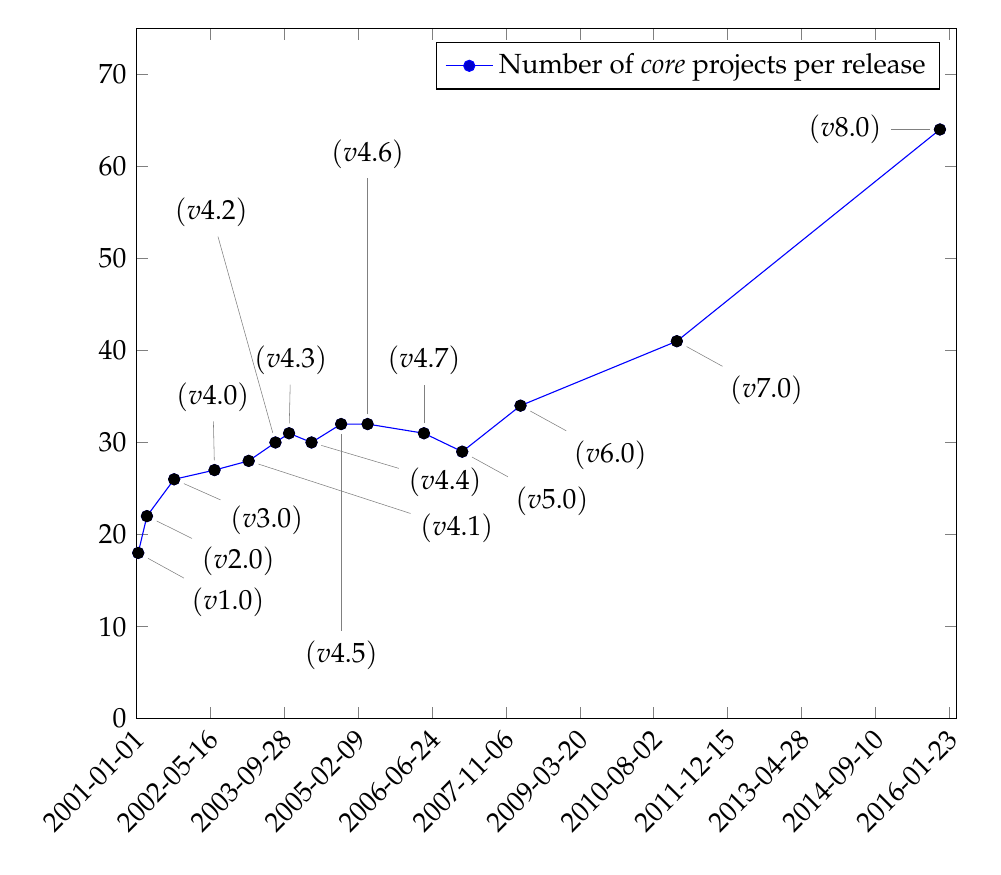
\begin{tikzpicture}
      \begin{axis}[width=12cm, date coordinates in=x,date ZERO=2001-01-01,
                   xticklabel=\year-\month-\day,ymin=0,ymax=75,
                   x tick label style={rotate=45, anchor=east, align=center, yshift=-5pt},
                   label style={font=\tiny},
           xmin=2001-01-01,
           xmax=2016-03-10]
       \addplot coordinates {
    (2001-01-15,18)
    (2001-03-15,22)
    (2001-09-15,26)
    (2002-06-15,27)
    (2003-02-01,28)
    (2003-08-01,30)
    (2003-11-01,31)
    (2004-04-01,30)
    (2004-10-18,32)
    (2005-04-15,32)
    (2006-05-01,31)
    (2007-01-15,29)
    (2008-02-13,34)
    (2011-01-05,41)
    (2015-11-19,64)
       };
       
\addplot[mark=*] coordinates {(2001-01-15,18)} node[pin=-30:{$(v1.0)$}]{} ;
\addplot[mark=*] coordinates {(2001-03-15,22)} node[pin=-25:{$(v2.0)$}]{} ;
\addplot[mark=*] coordinates {(2001-09-15,26)} node[pin=-20:{$(v3.0)$}]{} ;
\addplot[mark=*] coordinates {(2002-06-15,27)} node[pin=-268:{$(v4.0)$}]{} ;
\addplot[mark=*] coordinates {(2003-02-01,28)} node[pin={[pin distance=2cm]-15:{$(v4.1)$}}]{} ;
\addplot[mark=*] coordinates {(2003-08-01,30)} node[pin={[pin distance=2.5cm]-265:{$(v4.2)$}}]{} ;
\addplot[mark=*] coordinates {(2003-11-01,31)} node[pin=-272:{$(v4.3)$}]{} ;
\addplot[mark=*] coordinates {(2004-04-01,30)} node[pin={[pin distance=1cm]-10:{$(v4.4)$}}]{} ;
\addplot[mark=*] coordinates {(2004-10-18,32)} node[pin={[pin distance=2.5cm]270:{$(v4.5)$}}]{} ;
\addplot[mark=*] coordinates {(2005-04-15,32)} node[pin={[pin distance=3cm]-270:{$(v4.6)$}}]{} ;
\addplot[mark=*] coordinates {(2006-05-01,31)} node[pin= -270:{$(v4.7)$}]{} ;
\addplot[mark=*] coordinates {(2007-01-15,29)} node[pin=-30:{$(v5.0)$}]{} ;
\addplot[mark=*] coordinates {(2008-02-13,34)} node[pin=-30:{$(v6.0)$}]{} ;
\addplot[mark=*] coordinates {(2011-01-05,41)} node[pin=-30:{$(v7.0)$}]{} ;
\addplot[mark=*] coordinates {(2015-11-19,64)} node[pin=180:{$(v8.0)$}]{} ;   

    \legend{Number of \textit{core} projects per release}
    \end{axis}
    \end{tikzpicture}
        \caption[Number of \textit{core} projects per release]%
        {Number of \textit{core} projects per release. Based on data collected by \textcite{zoubi-history:2016:Online}. Retrieved \nth{10} March 2016, from \url{http://websolutions.hr/drupal-history}, under a CC BY-SA 2.0 license.}
        \label{core-modules-release}
    \end{figure}

\begin{figure}[H]
  \centering
   \includegraphics[scale=0.6]{graphs/lines_of_code_in_core}
   \caption[Number of lines of code in core per release]%
        {Number of lines of code in core (excluding comments and blank lines) for the latest five releases of Drupal, based on an infographic by \textcite{core-loc:2016:Online}. Retrieved \nth{10} March 2016, from \url{http://drupalmotion.com/article/drupal-code-base}.}
\label{loc-core}
\end{figure}

Nevertheless, the higher degree of centralisation cannot only be understood in technical terms, but also as intertwined with social aspects, such as the internal perceived greater value of contributing to Drupal core. Changes in Drupal core affect the global direction of the project and, as a consequence, they have also been subjected to higher degrees of quality assurance, while the power to carry out modifications in these digital commons have remained more centralised when compared to \textit{contributed} projects, and even more so when compared with \textit{custom} projects not shared within Drupal.org. This rigidity in the processes is also intertwined with a higher degree of legitimacy to carry out these changes, when compared with projects in the \textit{contributed} system and, consequently, an even higher degree when compared with the \textit{custom} system. The following quote by I\textunderscript{10} illustrates the idea of how being able to perform large modifications in core used to operate on the basis of trust generated around the informal network explained in the previous quote, and how changes required, and continue to require, a higher degree of legitimacy --- in the form of the approval of the project leader in this case:

\begin{quotation}
``[...] so I was sitting on the floor, in the party room [during DrupalCon Sunnyvale (2007)] that night. With this little netbook that I borrowed from the company [looking at documentation to propose a set of changes in core]. [...] And Dries comes by, sits down on the floor next to me. And... after I explained to him [the proposed changes] he said:  `Yes, this makes senses, go with it'. Wait... what, what? [LAUGHS]. [...] And, you know, at this point I think he knew who I was, because I had done enough bits and pieces over the last year or so. But, that kick in the pants to say: `OK, you have the project leader's blessing to do this big thing'. It was huge. And getting that... you know, a lot of people like to talk about Open Source: `You don't need permission to get involved', but you kind of do when you are doing it at a high level, when you are making large changes, you do need to have someone's blessing. [...] And that blessing did help."
\begin{flushright}\footnotesize{Drupal core developer and architect, M, 11 years.}\end{flushright}
\end{quotation}

Nevertheless, this does not imply that these processes were not affected by the general dynamics of formalisation and decentralisation previously described. A similar trend of decentralisation in decision-making could be observed over time as well, but this occurred in a more rigid environment, when compared with that of \textit{contributed} projects. The next quote, by I\textunderscript{9}, illustrates this increasing need to decentralise the decision-making processes --- most significantly during the transition from Drupal 7 to 8 --- due to the growth of the community, and its relationship to the increase in the degree of formalisation:

\begin{quotation}
``[...] And now, because it's so big and there's so many changes that there's no real way to do that informally. There needs to be a formal process, so that the people who are responsible for doing certain things know that they're responsible for it, and know how to get it done. And people know how to contact them to ask them to do these things that they are responsible for. So, it has been getting more explicit and better documented, just because the people who need to be doing these things, need to be able to do them [...] and that's because as we get bigger, and we have a reputation for helping people get involved with contributing to Open Source, we get a ton of new people who want to contribute."
\begin{flushright}\footnotesize{Drupal core developer and mentoring organiser, F, 8 years.}\end{flushright}
\end{quotation}

During the same interview, I\textunderscript{9} also explained how the trend towards increasing the degree of formalisation reached a higher degree than in the case of the \textit{contributed} system, which can be interpreted on the basis of these processes being subjected to the aforementioned higher degree of expected legitimacy as well as accountability to the community:

\begin{quotation}
``[...] So, the procedures have to be more formalised in order for it to be welcoming for new contributors. Because people need to know how we do things, who to talk to, and why. Otherwise, it looks like ... like you have to be part of the in-crowd, or you have to know certain people, or you have to be in a \textit{backchannel}, and that stuff is really bad. It will drive away new contributors. So the formalisation has definitely increased, and I think it's a really good thing. Both, for the people who have to do the things, so they realise what they have to do. We talk about how to do them, and we come to some kind of agreement and plan. And also, for the new people, so we aren't hiding anything. The information that they need in order to contribute is exposed to them."
\begin{flushright}\footnotesize{Drupal core developer and mentoring organiser, F, 8 years.}\end{flushright}
\end{quotation}

To further understand how the general dynamics of formalisation and decentralisation shaped the self-organisational processes related to the development of \textit{core} projects, the next sections will provide a more extensive description and analysis of key aspects. Following a structure similar to that of chapter \ref{sec:custom-to-contrib}, the focus will be placed firstly on how formalisation and decentralisation occurred in the general organisational aspects. With that goal in mind, the changes experienced in the transition between cores 7 to 8, the longest release period in the history of the community as well as with the highest number of contributors in terms of code committers, will be discussed. Secondly, a specific core initiative is presented and analysed, following a similar structure as in section \ref{subsec:contrib-day-by-day} for the case of \textit{contributed} projects, in order to illustrate how these changes in the general organisational aspects facilitated the empowering of part of the community to change the direction of the project.

\section{Core initiatives, leaders and gates: formalisation and decentralisation in core}
\label{subsec:dec-form-core}

While minor changes in \textit{core} projects are introduced via patches, the possibility to carry out large changes which affect the direction of the project are harder to achieve when compared to \textit{contributed} projects  and require a higher degree of legitimacy in the community. As illustrated in the previous section, in the early stages the process strongly depended on the closeness of an informal network. As the community continued to grow, these processes incorporated more formalised mechanisms to improve transparency, objectivity and monitoring of these peer-production processes. The most prominent examples of this formalisation can be found during the transition from Drupal 7 to Drupal 8 --- five years of development, a third of the life of Drupal --- , as I\textunderscript{8} explained:

\begin{quotation}
``[...] So Drupal 7 was released, and Drupal 8 was open for development. And Dries knew that he wasn't gonna be able to make decisions about everything. And there were a lot of big ideas, that he wanted to be changed for Drupal 8. So I think there were four or five big ideas, and he decided to pick initiative leads that would... like lead making those things happen. And then he could still be contacted for certain things, but initiative leads would have... the responsibility to organise, review, and maintain... to try to make these goals happen."
\begin{flushright}\footnotesize{Drupal core developer and mentoring organiser, F, 8 years.}\end{flushright}
\end{quotation}

These \textit{official} initiatives\footnote{See \url{https://www.drupal.org/node/2107085}.} entailed a significant increment in the degree of formalisation with respect to early stages --- including formal leaders, roadmaps and a reflection in the tools of the main collaboration platform (see figure \ref{core-initiative}).

\begin{figure}[H]
   \centering
   \includegraphics[scale=0.5]{img/online/core_initiative.png}
   \caption[Example of information about official core initiative in Drupal.org]%
   {Example of the information about an official core initiative in Drupal.org, in this case ``Multilingual". Retrieved \nth{20} April 2015, from \url{https://www.drupal.org/node/2107085}, under a CC BY-SA 2.0 license.}
\label{core-initiative}
\end{figure}

However, in congruence with the higher degree of centralisation in this socio-technical system of contribution, the process was still carried out in a prominent top-to-bottom way: based on the direct appointment of well-known Drupalistas by Dries. Although this initial step could be understood as a matter of simple delegation, it also opened up a large discussion about how these decisions should be made. For example, this was reflected in the creation of formal rules discussed by the community with regard to the governance of core \parencite{drupalorg-core-governance:2016:Online}, as well as a more formalised division of labour. The following quote by I\textunderscript{10} illustrates this dynamic of formalisation and its reflection in the division of labour (e.g. formal roles such as project owners, release managers or subsystem maintainers), rules (e.g. attributions of those roles and explicit governance of core) and artefacts (e.g. distribution of power to commit changes),  among others:

\begin{quotation}
``[...] And that triggered a very extensive debate, which sometimes got a bit more heated than it should have. But, in the end I think it was good to air some of those problems. So earlier that year, we pushed through a new formalised structure. [...] we have an actual release manager role. We have a... someone actively called a project owner, and that's Dries and \textit{Jane}. And we clarified what a subsystem maintainer can and cannot do, sort of. And there are people who are now specifically supposed to look after the big picture architecture: \textit{Roger} and \textit{Joe}. And give lots of those people commit access to help again keep the RTBC [Reviewed and Tested By the Community] queue short. [...] We are trying to increase the amount of structure.[...] You need to have, you know, local structures of control which are part of a larger picture."
\begin{flushright}\footnotesize{Drupal core developer and architect, M, 11 years.}\end{flushright}
\end{quotation}

Overall, this led to the definition of more clearly defined community boundaries, which also established more effective ways to provide modifications of the rules by those who are affected by them. In addition this trend shows how the individuals responsible for monitoring those commons, in accordance with collective-choice arrangements, were required to become more accountable to the community and transparency increased. The following excerpt, extracted from the personal blog of a core maintainer in the context of a discussion about contribution and influence, illustrates how these changes in the self-organisational processes operate on a day-to-day basis and their reflection in the artefacts:

\begin{figure}[H]
\centering
\includegraphics[scale=0.45]{img/quotes_replacement/contribution-influence-drupal-8.png}
\caption[Excerpt from the article ``Contribution, Influence, and Drupal 8"]{Drupal core maintainer, F, 8 years. Excerpt from the article ``Contribution, Influence, and Drupal 8". Retrieved \nth{11} March 2015, from \url{http://xjmdrupal.org/blog/contribution-influence-drupal-8}.}
\label{quote_core_influence}
\end{figure}

For example, the Core Gates \parencite{drupalorg-core-gates:2015:Online, drupalorg-core-gates-rfc:2015:Online}, to which the Drupalista referred, are essentially sets of ``checklists" in different areas such as performance, accessibility, documentation, usability and testing, which emerged in response to the need to define explicit quality assurance mechanisms in ways which these collective-choice arrangements can be created and modified by a wider amount of Drupalistas willing to participate. For instance, specific groups were created to participate in its elaboration. Each of them had long discussions joined by hundreds to thousands of participants, which varied depending on the specific gate \parencite{drupalorg-core-gates-testing:2015:Online, drupalorg-core-gates-performance:2015:Online, drupalorg-core-gates-accesiblity:2015:Online}. Furthermore, this process of formalisation facilitated decentralisation in the decision-making beyond \textit{official} initiatives\footnote{Further details on \textit{unofficial} initiatives are extensively discussed in section \ref{subsec:dec-core-initiative}.}. Overall, these changes illustrate how the possibility to perform large modifications in these digital commons, in other words the power to change the direction of the project, became more distributed and transited from depending on an informal network towards depending more on explicit sets of collective-choice arrangements discussed and formalised by the community. The following excerpt from I\textunderscript{8} summarises how the processes of decision-making scaled up and became more decentralised on the basis of this formalisation of policies:

\begin{quotation}
``[...] somebody decides we should have a policy about something, and then that policy is discussed, and then the policy is accepted. And then, once that policy is in place, it's easier to make a decision, about if this feature is gonna go in, or when it's gonna go in, or when are we gonna have a release, because we have a policy in place, which documents how we make those decisions. So, in general, the way Drupal makes decisions is like that. It tries to make a policy, and then make that policy public for discussion, come to a consensus, and then whenever we need to make a decision about something, we reference that policy, so it's not a secret."

\begin{flushright}\footnotesize{Drupal core developer and mentoring organiser, F, 8 years.}\end{flushright}
\end{quotation}

This is not to be confused with a romanticised picture in which the aforementioned consensus by I\textunderscript{8} is easily reached and there is complete egalitarianism. Large discussions are required to achieve it, and in cases of large conflicts, opinions from members with a higher reputation in the community are commonly taken into greater consideration, as found by \textcite{Zilouchian2011}. As stated by \textcite[67]{benkler2006wealth}, a hierarchy exists in these communities. However, as previously discussed in the case of \textit{contributed} projects, it differs radically from the types of hierarchy found in the traditional firm because of the peer-based nature of these communities. Hierarchies emerge and are legitimised on the basis of the ``do-ocratic" principles of these communities, while the dynamic of formalisation provides ways to allow the modification and participation in rules that become more explicit over time. This can be understood as a constant process of negotiation, in which it is common for tensions to emerge. I\textunderscript{5} illustrates how ``do-ocratic" principles shaped the day-to-day in core, while also describing the hierarchies in the form of ``temporal power" and ``stronger voices":

\begin{quotation}
    ``[...] And, after all, it's a community debate. Who has the best argument... or the most practical arguments sometimes, because it's really `do-ocratic': if you have tons of arguments but you don't have the code, it doesn't matter. But, in the end, the power to take a decision resides on each issue, or each group of issues, each of them having an opinion which could be pretty different to another issue or initiative. And there is a temporal power. People who spend a lot of time in a set of issues obviously have a stronger voice in there. But not on a global level, in which the initiative leaders' voices are stronger."

\begin{flushright}\footnotesize{Drupal developer and ex-member of the Drupal Association Board of Directors, M, 9 years. Original reply in Spanish.}\end{flushright}
\end{quotation}

The evolution of these processes illustrates how the necessity of scaling up also entailed a dynamic of formalisation in order to decentralise the decision-making in the socio-technical system of \textit{core} projects. While the degree of decentralisation is lower than in the case of the \textit{contributed} socio-technical system, a trend of decentralisation can also be observed over time. Although, this results in a system characterised by a lower degree of autonomy, a higher degree of quality assurance in their peer-production processes, as well as a higher degree of legitimacy in order to govern these digital commons and perform changes in them. In order to further understand how these general dynamics of formalisation and decentralisation operate at a more micro level, the next section provides a case study of one of these core initiatives.

\section{Case study: the story of an \textit{unofficial} core initiative}
\label{subsec:dec-core-initiative}

This section focusses on ``Twig in Core", a core initiative aimed to radically change the way in which contents were output by Drupal. Several factors made this initiative particularly interesting. Firstly, this is one of the initiatives not officially appointed by Dries, thus allowing the illustration of the transition of initiatives which emerged from the community in a bottom to top way, therefore more prominently demonstrating how the general dynamic of decentralisation operated in the socio-technical system of \textit{core} projects. Secondly, ``Twig in Core" was an initiative led by and of particular significance for frontend developers or themers\footnote{The use of the word frontend developer or themer is typically interchagable in the community. However, a tendency towards a preference of the usage of the term frontend developer when referencing themselves was appreciated during participant observation. When asked, several themers explained they preferred it because the  inclusion of the term developer explains their work with source code more explicitly. Overall, the perceived strong value which the word ``developer" has in the community could be explained as responding to the general ``code-centric" culture discussed in chapter \ref{identifyng-contribution:chapter}.}, a Drupal role depicted in \citeauthor{Zilouchian2011}'s study (\citeyear{Zilouchian2011}) as suffering a lack of power in decision-making due to the community's ``code-centric" character. Finally, the scope of this initiative was not only limited to the inclusion of ``Twig in Core", but it became an \textit{umbrella} initiative for various changes related to the frontend of Drupal, and remains even after Drupal 8 was officially released. Hence, the study of this initiative will not only provide a better understanding of how the aforementioned dynamics of formalisation and decentralisation operate at a micro level, but it will illustrate the role that the changes in the general organisational processes played to empower some of these groups of Drupalistas.

\subsection{The scratching of the themers' itch: ``Twig in Core"}
\label{subsec:themers-itch}

The origin of the ``Twig in Core" initiative can be traced to the need expressed by themers to provide Drupal with a theme engine\footnote{A theme engine is ``a collection of scripts and files that interact with the core and interpret the programming language used in the theme" \parencite{theme-engine:Online}. They provide easier ways to separate output into templates, with the aim of separating the logic layer from that of presentation. A theme is a collection of files that define the presentation layer \parencite{theme:Online}.} which fulfils their needs. Since version 4.7, released in 2006 \parencite{drupal_4_7:Online}, and up to the release of Drupal 8 (November 2015), PHPTemplate was the default theme engine in Drupal core. The use of PHPTemplate as a theme engine for Drupal started as an experimental project in the \textit{contributed} system in 2004 \parencite{phptemplate:Online}. Its main aim was to allow the use of template files written in pure PHP, providing flexibility and secure access to any information available via Drupal's API. This theme engine was shaped by the architectural perspectives of backend developers, as depicted by the emphasis on security, however, over the years a growing number of themers argued that the theme engine did not fulfil their needs.

This example of tension within the division of labour --- Drupal roles --- and the object --- Drupal core --- was significant considering that, as commonly expressed by many Drupal themers, they are those who work more closely with the theme engine, since their main job typically consists of translating a graphic design into a Drupal theme. Some of these regular complaints from themers about the theme engine relate, for example, to the way in which HTML code was produced by Drupal's core. For instance, there were complaints about Drupal suffering from ``divitis", referring to the  excessive amount of div\footnote{A div is a common HTML tag which defines a division or a section in an HTML document \parencite{div:Online}.} elements created by Drupal's theme engine. Another example was a critique of the ``the class soup" generated by Drupal, referring to the excessive amount of CSS\footnote{CSS (Cascading Style Sheets) is a language to ``describe how HTML elements are to be displayed on screen, paper, or in other media" \parencite{css:Online}.} files and their chaotic structure, due to the way this theme engine shaped the theming architecture overall. Figure \ref{divitis} depicts a slide during a keynote of a \textit{DrupalCamp} entitled ``The Angry Themer", illustrating the expression by themers of  these unfulfilled needs in sarcastic and humorous ways, in line with this characteristic of hacker culture \parencite[116]{coleman2013coding} previously discussed.

\begin{figure}[H]
  \centering
\includegraphics[scale=0.42]{img/online/divitis_morten_dcnw2012.png}
\caption[Screenshot from keynote ``The Angry Themer" at \textit{DrupalCamp} North West 2012]%
{Example of the complaints about ``divitis" from Drupal themers as illustrated during \textit{DrupalCamp} North West 2012 keynote: ``The Angry Themer". Retrieved \nth{10} November 2016, from \url{https://vimeo.com/54387556}, under a CC BY-SA 2.0 license.}
\label{divitis}
\end{figure}

The existence of this tension between division of labour and the object was explained by Drupalistas to be due to a lack of communication between backend and frontend developers. The following excerpt, extracted from the same presentation, illustrates this tension:

\begin{quotation}
``[...] [During a social event in DrupalCon Denver (March, 2012)] I was out on the way to the car, and I was bitching and moaning to webchick [backend developer and core comitter]: `How the fuck? Why don't you give us the markup we want? Why can't I change everything?'. And at some point, I think she just got tired of me, like, looked at me, those kind of eyes, like... `Morten, nobody told us what to do!' And I am like...`Eh? But I have been telling you guys that for years'. [EXPLAINING HER ANSWER] `Well, nobody told anybody in the development community what to do'."
\begin{flushright}\footnotesize{Extracted from \textit{DrupalCamp} North West 2012 keynote: ``The Angry Themer" (14'.58" - 15'.20"). Retrieved \nth{18} November 2016, from \url{https://vimeo.com/54387556}, under a CC BY-SA 2.0 license.}\end{flushright}
\end{quotation}

In the context of the same presentation, this Drupalista also explained the passive role of frontend developers in the early stages:

\begin{quotation}
``[...] Eight years ago there was nobody [referring to the themers], six years ago I think there was just me and one other, ... five years ago we were maybe ten, three years ago in DC [referring to DrupalCon DC (March, 2009)] there was a bunch of us... so this is also a blame on the frontend community, that nobody told anybody in the backend or the development community what is it that we wanted [...] So at this point you can choose two different ways: either you can be bitching and moaning [...] or you can try to figure out how can we work around this."
\begin{flushright}\footnotesize{Extracted from \textit{DrupalCamp} North West 2012 keynote: ``The Angry Themer" (15'.20" - 16'.12"). Retrieved \nth{18} November 2016, from \url{https://vimeo.com/54387556}, under a CC BY-SA 2.0 license.}\end{flushright}
    \end{quotation}

The consequences of this tension between division of labour and the object can be interpreted as generating an ``itch to be scratched" \parencite{torvalds2001just} by themers. As illustrated by the previous quote, some of them started to organise themselves in 2006 \parencite{morten-history:Online}. These initial efforts were firstly discussed and materialised in the \textit{contributed} system, not surprisingly due to the higher degree of flexibility and experimentality which characterises it. This is illustrated, for example, by the development and release in 2009 of modules such as Style Stripper \parencite{styletripper:Online}, or base themes\footnote{A base theme is a basic theme providing a small amount of style which can be used as a wireframe or template to build other themes on top of it \parencite{base-theme:Online}.} such as Mothership \parencite{mothership:Online}, which provided ways to clean up the excessive markup generated by Drupal's theme engine in the themers' eyes, and offered them more control over their work. Hence, an emergent progression towards an active role of frontend developers can be observed. The following excerpt, by I\textunderscript{15}, provides an overview of the emergence of these initiatives in the socio-technical system of \textit{contributed} projects at the time, the more active role taken by some frontend developers, and the relevance of building a reputation through contributions in order to be able to participate in changes in core:

\begin{quotation}
``[...] Drupal 6 [February, 2008] came out, and I remember looking at the theme system: [...] `Why do we have so much markup?!' [...] So eventually I developed a theme called the `Mothership'. First of all, because I learnt that you can bitch and moan about the system as much as you want, but in Open Source talk is pretty much nothing, code is the currency we live by [...] . And there's also a social economy around this. [...] [When you go to a Drupal event] you want to talk about the module you're building, the theme you build, the project you build. That's your currency. [...]"
\begin{flushright}\footnotesize{Drupal frontend developer, M, 10 years.}\end{flushright}
\end{quotation}

While these \textit{contributed} projects provided partial solutions to the problem, themers felt these changes were so relevant that they should be implemented in the heart of Drupal. However, as previously discussed, changes in core are more difficult to achieve because of the high level of legitimacy necessary to perform those changes, the high quality standards and strong peer-reviewing processes, as well as the high level of complexity and interdependency of the object, among other factors. In addition, the degree of the themers' self-organisation was significantly low at the time, and their voices were also less heard in the community \parencite{Zilouchian2011}. The following anecdote reported by I\textunderscript{15}, regarding frontend developers running a parallel set of frontend sessions during DrupalCon DC (March, 2009), depicts the situation at the time:

\begin{quotation}
``[...] There was only two frontend sessions. There was me and \textit{Matthew}, the maintainer of the [core] theme system [...]. Both of us got pissed off: `Why there is only two sessions about the frontend? How can ...? Apparently everything else matters so much more, but actually how sites are built is not relevant from the developer perspective'. [...] So, \textit{Matthew} asked all the people who submitted sessions, and they submitted them to him, and he picked out 20 [frontend rejected] sessions, [...] and he took one of the BoF [Birds of a Feather] whiteboards, and put the whole program and say: `This room in there is the frontend room, and, by the way, you can all go fuck yourselves' [LAUGHS]. That was pretty much the attitude."
\begin{flushright}\footnotesize{Drupal frontend developer, M, 10 years.}\end{flushright}
\end{quotation}

In the context of the same anecdote, I\textunderscript{15} explains how a more empowered group of frontend developers began to emerge:

\begin{quotation}
``[...] Suddenly, I realised it was not only me and \textit{Matthew}: we had a ton of people coming and willing to talk about what to do about this [referring to changing the frontend]. [...] [Months later] I was beginning to know a lot people [...], these connections started to be made, and we came up with an idea: `let's do a frontend conference' [...]"
\begin{flushright}\footnotesize{Drupal frontend developer, M, 10 years.}\end{flushright}
\end{quotation}

During the next years frontend developers started to organise themselves in more regular and formal ways \parencite{d4dgroup:Online}. The emergence of the initiative, as depicted by the previous quote, went beyond the online limits. As observed during my participation and emphasised by all the Drupalistas interviewed about the initiative, F2F events played a significant role in fostering the initiative\footnote{The socio-technical systems of Drupal events are extensively described and analysed in chapters \ref{mostly-offline-local:chapter} and \ref{mostly-offline-cons:chapter}.}. These events, originally known as D4D or Drupal Design Camps emerged in Boston in 2009 \parencite{d4dcamp:Online}, and were extended to Europe in 2010 \parencite{d4dcamp_eur:Online}. In 2012 they were renamed as ``Frontend United" \parencite{fe_united:Online}, one more example of how this increasing sense of empowerment and self-determination was reflected, including in the naming of the events themselves. Picture \ref{frontend-united-2012} depicts the first ``Frontend United" meeting in Amsterdam in April 2012, with more than 200 attendees according to the statistics offered by the event organisers, and picture \ref{frontend-united-symbol} illustrates the use of specific symbology by the group.

\begin{figure}[H]
\centering
\includegraphics[scale=0.6]{img/online/group-photo_fu_2012.jpg}
\caption[Group photo during Frontend United 2012]%
{Group photo during Frontend United 2012, in Amsterdam. Retrieved \nth{14} November 2016, from \url{https://www.flickr.com/photos/elv/6952927548/in/photostream/}, published by Philippe Gervaise, under a CC-BY-SA license.}
\label{frontend-united-2012}
\end{figure}

\begin{figure}[H]
  \centering
\includegraphics[scale=0.3]{img/online/fe-united-logo.jpeg}
\caption[Picture of a ``Frontend" T-shirt]{An example of the development of symbology for the group of Drupal themers. In this case, a ``F" standing for Frontend. Retrieved \nth{14} November 2016, from \url{https://twitter.com/frontendunited/status/781988434583879680} by @frontendunited.}
\label{frontend-united-symbol}
\end{figure}

With the rise of core initiatives for Drupal 8 presented in section \ref{subsec:dec-form-core}, frontend developers envisioned an opportunity to implement these changes in Drupal's core. They organised themselves around ``Twig in Core", an unofficial core initiative named after the decision to include the FLOSS template engine Twig\footnote{Twig \parencite{twig-doc:Online} is a FLOSS template engine for PHP inspired by Python engines such as Jinja \parencite{jinja:Online} or Django's engine \parencite{django:Online}. It consists of an intermediate layer which allows the effective separation of the presentation layer from the logical one, creating faster and more secure PHP code, and providing more control for template designers, in this case Drupal themers. It is also employed by several popular FLOSS projects such as Symfony, phpBB or Piwig among others.}. The following quote, by I\textunderscript{15}, provides an overview of some of the most relevant events at the time:

\begin{quotation}
``[...] In [Frontend United] Amsterdam [2012], we were doing brainstorms on how the system should work [...] And \textit{Peter} [a well-known Drupal developer who was looking at the issue while attending a parallel Drupal event in San Francisco] came up with the idea of using Twig [...]. And there were 200 frontenders there [in Amsterdam]... and we had no fucking idea what Twig was. But there was this one dude... `I know about Twig, I can do a clone and show you how it can do things more elegant [...]'. So he showed it to us ... and it made a lot of sense, because it made the system more elegant but also secure. It was a kind of match, [...] because for [backend] developers it made the system more secure [implying this is one of the most relevant aspects for them]. [...] So [to include Twig] we would need to write everything: convert every single function into a template. [...] And I was like: `OK, this is good. If we force ourselves to do this, we cannot have Drupal 8 out of the door before we finish all this work'. So, to me, that was a kind of pact with the Devil. [...] And we started having weekly meetings. [...] Several people started jumping in, [...] and we suddenly start to have a small group of people who were showing up every week. [...]"
\begin{flushright}\footnotesize{Drupal frontend developer, M, 10 years.}\end{flushright}
\end{quotation}

These excerpts illustrate the emergence of a more formal and organised group of frontend developers to carry out  these changes in core; hence depicting a progression over time from a passive position, as the one described by \textcite{Zilouchian2011} or the initial period referred to in previous quotes, to an active one. Rather than relying on lobbying techniques \parencite{Zilouchian2011}, they self-organised around an initiative, also including backend developers, to produce these architectural changes in core. This progression can be interpreted as a growing form of self-empowerment of frontend developers in the community.  The following excerpt by a Drupalista who joined the initiative at the time, extracted from a comment on a blog post on authority and FLOSS, provides an overview of this increasing degree of self-empowerment in the group, as well as how decentralisation in decision-making and rotation in leadership characterised the subsequent stages in organisational terms within the initiative:

\begin{figure}[H]
 \centering
 \includegraphics[scale=0.5]{img/quotes_replacement/quote_twig_cc.png}
 \caption[Excerpt (I) from comment in the article ``On authority in Drupal and/or Open Source in general"]{Drupal core committer, M, 4 years. Excerpt (I) from comment in the article ``On authority in Drupal and/or Open Source in general". Retrieved \nth{15} March 2015, from \url{http://hojtsy.hu/blog/2014-oct-17/authority-drupal-andor-open-source-general}, under a CC BY-SA 2.0 license.}
\label{quote_twig_core_01}
\end{figure}

A key moment for the initiative occurred when Twig was committed to core during a \textit{DrupalCamp} in November 2012 \parencite{badcamp2012:Online}. The commit was carried out as a ``live commit", a gathering of Drupalistas during F2F events in which commits are publicly pushed as part of a community celebration, also providing public acknowledgement of contributions. Picture \ref{twig-core} shows the euphoria of one of the main leaders of the initiative during the live commit, a culmination of all the hard work carried out by the initiative up to that point.

\begin{figure}[H]
\centering
\includegraphics[scale=0.45]{img/online/twig_in_core.jpg}
\caption[Pictures from the committing of ``Twig in Core" during BADCamp 2012]%
{Jen Lampton --- the Drupalista in the middle of the picture joining her hands ---, one of the most visible leaders of the `Twig in Core' initiative at the time, watches as Twig is committed to Drupal core live during the BADCamp 2012. Picture by Ezra Barnett Gildesgame retrieved \nth{22} November 2016, from \url{https://www.flickr.com/photos/ezrabg/8155887186/}, under a CC-BY license.}
\label{twig-core}
\end{figure}

\subsection{Self-organisation, decentralisation and empowerment within a core initiative}

As presented in the previous section, frontend developers progressed from a passive to an active position, and self-empowered and organised themselves to create an initiative which would change the direction of the Drupal project. In the subsequent years, this led to the development of a more formalised group, which in the eyes of some of the participants was even a sub-community within Drupal, as illustrated by the following excerpt by I\textunderscript{15}:

\begin{quotation}
``[...] [Twig in Core] has been pretty much about building a community on the side. We now have this Twig Slack\footnote{See \url{http://drupaltwig-slack.herokuapp.com}.} channel with more than 600 people. That was pretty much the approach: building a community that can help the Drupal community. Because we couldn't build it inside of Drupal, because inside of Drupal... it was so much built on engineering and development. And we wanted to talk design and implementation. [...]"
\begin{flushright}\footnotesize{Drupal frontend developer, M, 10 years.}\end{flushright}
\end{quotation}

This process entailed the development of an environment which facilitated decentralisation of decision-making and fostered a sense of empowerment in the participants, as illustrated by the following excerpt from the interview with I\textunderscript{14}, who became an active member in the initiative at the time and led it for almost a year:

\begin{quotation}
``[...] it was totally a grassroots initiative, it was just people trying to do things better. Especially, if you go later on in Twig in Core in 2013, 2014, and so on, then... what you see is the larger Drupal frontend community behind this thing, and really helping to try to push it forward, even if they're not sure they have the skills to do so, but having the passion, the enthusiasm and the desire to push this change. I think that's how it was successful, it wouldn't have been successful if it was just the same four or five people working on it for years, that's just not enough, it needed a bigger community, it needed that support. [...]"

    \begin{flushright}\footnotesize{Drupal frontend developer, and core committer after the initiative, M, 6 years.}\end{flushright}
    \end{quotation}

During the following years, the initiative evolved within an organisational environment with internal and external tensions, which were reflected in the entities surrounding its organisational processes. On one hand, the high interdependency of the object required an almost full version, since a partial one would make Drupal core unshippable\footnote{The term unshippable, in the context of software development, refers to an unfinished version affecting some of the critical functionalities.}. This was a source of tensions, which at several points brought into question the future sustainability of the initiative, and even the legitimacy of the changes to remain in core. For example, the following excerpt by I\textunderscript{14} illustrates some of these external tensions, in which it was discussed whether Twig should be rolled back:

\begin{quotation}
``[...] in a way we needed to almost sell it to Dries and to the core committers and say: `We know this isn't an official initiative, but, you know, we hope you agree that it's a good thing' [...]. So I met Dries for the first time at DrupalCon Portland [May, 2013], ... and I just remember him asking things like [...]: `If the Twig team went away, would you still want Twig in Core?', like, `Would you still put it in core?'. So I think, there's a lot into that, I think, but part of what he was asking is like: `Is this something that people can and will maintain? Or is it just like your baby that, you know, you're putting into core?' [LAUGHS]. [...] we had to do the work first [...], so in [DrupalCon] Portland [May, 2013] basically what happened is if we didn't meet the deadline, if we didn't have everything go in all at once [...] Drupal would have been in a less shippable state, let's say, because if we would just have converted [the existing templates] one by one, [...] if you end up shipping Drupal with half PHP templates and half Twig... that's not good [LAUGHS]. [...] It needed to be full, kind of comprehensive. Otherwise it would've never worked, and we would've just had to roll it back [...]"

\begin{flushright}\footnotesize{Drupal frontend developer, and core committer after the initiative, M, 6 years.}\end{flushright}
\end{quotation}

On the other hand, there was a lack of consensus at the time within the group regarding the way in which the philosophy of the new theming system should be implemented, also producing internal tensions. A survey\footnote{Unfortunately, no sources could be found regarding the survey design beyond an interview in a Drupal podcast \parencite{twig-morten-interview:Online}. During the interview with I\textunderscript{15}, the Drupalista most heavily involved in the survey design and dissemination, he reported the survey was taken by more than 500 Drupal frontend developers, and it was mainly distributed via social networks and frontend developers channels.} designed and disseminated by the group showed what at the time seemed to be two mutually-irreconcilable positions. On one hand, around a third of the themers who participated in the survey were in favour of a completely clean system, lacking default divs and CSS. On the other hand, the two remaining thirds preferred a system with a cleaner but substantial default amount of them.  A key moment for the group to reach a consensus in the initiative occurred during DrupalCon Austin (June, 2014), in what was known as the ``consensus banana" -- picture \ref{consensus-banana} depicts a picture taken around the famous banana.

\begin{figure}[H]
\centering
\includegraphics[scale=0.6]{img/polycentric/consensus-banana.jpg}
\caption[Group picture of the participants in the ``consensus banana" BoF at \textit{DrupalCon} Austin 2014]%
{A group picture of the participants in the BoF of the ``consensus banana", another humorous form characteristic of the hacker culture \textcite{coleman2013coding}. Picture retrieved \nth{22} September 2016, from \url{https://www.drupal.org/files/issues/consensus-banana.jpg}.}
\label{consensus-banana}
\end{figure}

The consensus banana refers to a popular story within the Drupal community in which, during a BoF in \textit{DrupalCon} Austin 2014, frontend developers employed a banana as a pointer stick to try to push forward decision-making and reach a point of consensus for the philosophy of the new theming system. That point of consensus was reached by the creation of two themes representing both philosophies: ``classy" and ``stable". The default behaviour of the system would be to reduce the markup as much as possible, drawing on the base theme,``stable", but core would also be shipped with ``classy", another base theme which provides classes to help annotate markup elements. Several outcomes were produced as part of this episode as well, such as a more formalised roadmap for the initiative \parencite{consensus-banana:Online}. The following excerpt, extracted from the same previous comment, summarises this episode and some of its main outcomes:

\begin{figure}[H]
\centering
\includegraphics[scale=0.5]{img/quotes_replacement/quote_twig_cc2.png}
 \caption[Excerpt (II) from comment in the article ``On authority in Drupal and/or Open Source in general"]{Drupal core committer, M, 4 years. Excerpt (II) from comment in the article ``On authority in Drupal and/or Open Source in general". Retrieved \nth{15} March 2015, from \url{http://hojtsy.hu/blog/2014-oct-17/authority-drupal-andor-open-source-general}, under a CC BY-SA 2.0 license.}
\label{quote_twig_core_02}
\end{figure}

Beyond the technical issues related to this consensus, the interesting part for this study is in the changes experienced in the organisational processes over time in this core initiative. Under an increasing need to scale up decision-making, a higher degree of formalisation was experienced in the self-organisational processes and reflected in the most relevant entities. For example, a more formalised and explicit set of rules were defined by the group, as illustrated by the creation of the roadmap, the definition of the initiative principles \parencite{twig-core-guidelines:Online}, and the participation through public periodic recorded calls\footnote{See \url{https://www.youtube.com/user/jenlampton/videos} and \url{https://www.youtube.com/channel/UCl51NoedmaLaaZg3pu1jmCQ/videos?shelf_id=0&view=0&sort=dd}.}. Similarly, it was also reflected in the main artefacts employed for collaboration, as depicted by the creation of specific platforms for the initiative --- see figure \ref{drupaltwig} as an example --- and by the usage of surveys to collect feedback from the community.

\begin{figure}[H]
\centering
\includegraphics[scale=0.3]{img/online/drupaltwig.png}
\caption[Screenshot of DrupalTwig.org]%
{Partial screenshot of DrupalTwig.org (\url{http://drupaltwig.org/}), depicting the novice section, with issues tagged as novice-friendly. Retrieved \nth{28} November 2016, from \url{http://drupaltwig.org/issues/novice}.}
\label{drupaltwig}
\end{figure}

In addition, formalisation was reflected in the division of labour, as depicted by more explicit roles regarding leadership, which rotated over time, and a more explicit definition of roles for the day-to-day work on the issues. The following quote from the interview with I\textunderscript{13}, who joined the initiative after the `consensus banana' and ended up leading it a year later, depicts some of the main organisational characteristics during this period:

\begin{quotation}
``[...] I got involved at the consensus banana time [March, 2014][...]. In the beginning \textit{Josh} created an agenda, he would have, like, a list of issues to discuss in the call [...]. I started running it in 2015, and we started doing this with a more community approach. Everyone who wanted to participate would create their own, like..., role. So there was a template: `I will be working on these issues, [...]'. And there was another section: `These issues need attention' [...]. So it became a bit more community-oriented and we got more momentum because of that."

\begin{flushright}\footnotesize{Drupal backend and frontend developer, M, 6 years.}\end{flushright}
\end{quotation}

I\textunderscript{13} also explained how this affected decision-making processes, and the distribution of power and rotation in the leadership:

\begin{quotation}
``[...] Obviously it was always very, very consensus-based. Finding consensus isn't always easy, but everything was consensus-based. So there was never only one person making decisions, [...] [those leading the initiative at each point] were not trying to force any issues. [...] We discussed a lot of these things in the meetings, the issue lists... and also the big decisions were done during DrupalCons, [...] and there was definitely rotation [in the leadership]. During each cycle, only maximum of one year, ... less than one year per person who was kind of the person trying to lead the team. [...] There was a very specific core team all time, ... there was new people who got in. [...] The size of the [core] team, in the end became bigger, even if people were leaving that crew, but it was never getting smaller at any point until Drupal 8 got released. [...]"

\begin{flushright}\footnotesize{Drupal backend and frontend developer, M, 6 years.}\end{flushright}
\end{quotation}

The previous excerpt illustrates the existence of a core team within the initiative, in congruence with the common distribution in participation found in many other CBPP communities discussed in section \ref{sec:cbpp-research}; but most importantly, how the initiative was also characterised by a significant degree of rotation in leadership, in which an essential aim was to hear participants' opinions. It can be observed how, within the initiative, power was distributed and loose even from those leading the initiative at previous stages. For example, with regard to decision-making related to the architectural design and philosophy of the new engine, the following excerpt, also extracted from the previous comment by a Drupalista leading the design during the stage before the ``consensus banana", provides an illustration of this distribution of power, rotation and decentralisation of decision-making within the initiative:

\begin{figure}[H]
\centering
\includegraphics[scale=0.5]{img/quotes_replacement/quote_twig_cc3.png}
 \caption[Excerpt (III) from comment in the article ``On authority in Drupal and/or Open Source in general"]{Drupal core committer, M, 4 years. Excerpt (III) from comment in the article ``On authority in Drupal and/or Open Source in general". Retrieved \nth{15} March 2015, from \url{http://hojtsy.hu/blog/2014-oct-17/authority-drupal-andor-open-source-general}, under a CC BY-SA 2.0 license.}
\label{quote_twig_core_03}
\end{figure}

The analysis of the data collected for the study of this initiative reveals the relevance that the sense of empowerment of frontend developers had to carry out the initiative successfully. The following excerpt, from the interview with I\textunderscript{12}, provides an illustration of this relevance, and how it was extended by, and within, a constantly growing group of frontend developers involved in ``Twig in Core" during this ``post-consensus banana" period:

\begin{quotation}
``[...][in the beginning] it was basically \textit{Jorgen} empowering us... [...] and then we took that message: `We can make the frontend better. We can take this and have the power to improve it!' [...] And \textit{Jorgen} was the main person who went around the World saying it, and then we all did that as well. [...] I don't think an initiative like this would have been possible five years ago, ... there was just not enough of us [frontend developers]. He empowered a few of us, and then we took that, and empowered a handful more people, ten people, it kind of grew from there. And at every event we had more people joining in ... it was incredible. I don't know how all these tables and tables of people [referring to Drupalistas contributing to the initiative during code sprints held at events] ... it just grew over the last few years. [...]"

\begin{flushright}\footnotesize{Drupal frontend developer, F, 4 years.}\end{flushright}
\end{quotation}

\subsection{Release of Drupal 8 and beyond}

The release of Drupal 8 on 19th of November 2015 \parencite{d8-release:Online} represented, among many other major changes in Drupal's core, the culmination of the work carried out by the ``Twig in Core" initiative. After years of work to tackle this  ``scratch to be itched" by frontend developers, the frontend of Drupal was completely changed. The following excerpt, extracted from the abstract of a presentation during the last \textit{DrupalCamp} Florida (March, 2016), shows this sense of fulfilment of the Drupal frontend developers with the changes achieved by the initiative:

\begin{figure}[H]
\centering
\includegraphics[width=\textwidth]{img/quotes_replacement/dcamp_session_twig.png}
\caption[Excerpt from abstract of session ``Twig \& Drupal 8 Theming" in Florida \textit{DrupalCamp} 2016]{Excerpt from abstract of session ``Twig \& Drupal 8 Theming" in Florida \textit{DrupalCamp} 2016. Retrieved \nth{20} March 2016, from \url{http://2016.fldrupal.camp/sessions/approved/florida-drupalcamp-2016/design-theming-front-end-development/twig-drupal-8-theming/index.html}.}
\label{dcamp_session_twig}
\end{figure}

Beyond the massive technical changes in the object, Drupal core, the previous excerpt also depicts the relevance of the fact that they were driven by those who are most intimately working with this part of the system. Furthermore, when discussing what the most important outcomes achieved by the initiative were with the Drupalistas interviewed, they commonly highlighted the creation of a consolidated group of frontend developers which successfully managed to change the direction of the project, and remains doing so even after the launch of Drupal 8. The following excerpt, from the interview with I\textunderscript{15}, illustrates the relevance of these less visible outcomes in the eyes of Drupalistas:

\begin{quotation}
``[...] creating a place where we could kick that stuff out, and self-organise to build this... it's kind of the ultimate scratch to be itched out. [...] creating a plan, creating a structure, building a community around, bringing in enough people, ... it [the initiative] was way more than creating 600 issues, it was about learning how to organise people around it, [...] now there is a few [frontend] initiatives around. [...] so if you go to our Slack channel [CHECKING THE LINK]... we have 616 users registered on the Twig Slack channel. Of course a lot of them are not active, but that's at least...  that crew means that we have something going on. That it was not completely wrong when \textit{Matthew} took over one BoF room in DC 2009, and said, you know: `We are going to take this over'."

\begin{flushright}\footnotesize{Drupal frontend developer, M, 10 years.}\end{flushright}
\end{quotation}

Overall, this case study illustrates how the dynamics of formalisation and decentralisation that shaped the general organisational processes presented in section \ref{subsec:dec-form-core} operate and materialise at a micro level by carrying out an in-depth study of one of these core initiatives. ``Twig in Core" illustrates how groups of Drupalistas managed to successfully organise themselves to change the global direction of the project. They progressed from a passive position, characterised by requesting changes, to an active one, in which they became accountable for and organised themselves to effectively implement them. As previously presented, the case of this initiative is not unique. While seven official core initiatives were originally proposed by Dries \parencite{d8-official-initiatives:Online}, during the development of Drupal 8 there was a total of 22 initiatives \parencite{d8-all-initiatives:Online}. Although there are differences between these initiatives, for example in their number of participants or whether they were official or not, they all occurred within a general organisational environment which, as depicted in section \ref{subsec:dec-form-core}, tended towards its formalisation, facilitating the decentralisation of decision-making to scale up these processes. Initiatives like ``Twig in Core" should be understood in this context, in which the process of formalisation of some of the entities, such as the rules for whether a project should or should not be part of core, act as an arena to foster initiatives to carry out these changes, in this case even by a group of Drupalistas which had previously had a lesser voice in the community \parencite{Zilouchian2011}. Furthermore, the case illustrates how the aforementioned dynamics also shaped the self-organisational processes of these initiatives. The following quote, in the context of a discussion of the main organisational aspects of these initiatives, shows Dries's views, shared by numerous Drupalistas, on how this degree of decentralisation played a relevant role in the success of the initiatives:

\begin{figure}[H]
\centering
\includegraphics[width=\textwidth]{img/quotes_replacement/power_self_managed_teams.png}
\caption[Excerpt from the article ``The power of self-managed teams in Drupal"]{Excerpt from the article ``The power of self-managed teams in Drupal". Retrieved \nth{3} May 2016, from \url{http://buytaert.net/the-power-of-self-managed-teams-in-drupal}.}
\label{power_self_managed_teams}
\end{figure}

Furthermore, this case study sheds light on the relevance which less visible outcomes had in the life of the community.  As previously illustrated, the outcomes of core initiatives went not only beyond the changes carried out in the object, but they represent the emergence of self-empowered groups which effectively changed these digital commons, following a general dynamic of decentralisation in decision-making even in the most rigid of the socio-technical systems of contribution with respect to the development of projects in the community. As depicted by the previous quote by I\textunderscript{15}, the process continues, and the emergence of these hubs of coordination are already defining the future of Drupal 9's core, through new core initiatives \parencite{d8-new-initiatives:Online}, some of them \parencite{d8-new-theme-in-core:Online} focussed on frontend issues as in the case of ``Twig in Core".

\section{Conclusion}
\label{mosly-online-discussion}

This chapter explored the emergence and main organisational changes of the socio-technical system of \textit{core} projects, the technical heart of the Drupal project. Overall, these changes resulted in a socio-technical system shaped by a ``do-ocratic" culture and characterised by a high degree of perceived internal value of the contributions made to these digital commons, whose quality assurance processes are the most strict and formalised of those identified for ``mostly-online" contribution activities, and changes to which require the highest degree of legitimacy in the eyes of the community, since they affect the general direction of the project.

Subsequently, it was explored how the general dynamics of formalisation and decentralisation operated at a macro level in this socio-technical system, as reflected, for example, in the division of labour, rules and main artefacts employed for collaboration; and how this was intertwined with a general trend towards decentralisation in the decision-making similar to that explained for the case of \textit{contributed} projects, although resulting in a socio-technical system that remained more centralised and with a lower degree of autonomy when compared with that of \textit{contributed} projects.

Finally, the focus was placed on how the aforementioned dynamics operated at a more micro level by exploring a core initiative, showing how these dynamics of formalisation and decentralisation are intertwined in the day-to-day, resulting in a more structured group in which the aim was to hear all participants' opinions and leadership was under rotation. Furthermore, this case study also illustrated the connection between the changes experienced in the general organisational aspects, at a macro level, with the emergence of initiatives themselves at a micro level, illustrating how they provided a scenario that facilitated the empowerment of a group of Drupalistas, whose voices had traditionally been less heard, to change the direction of the project.

Having explored all different socio-technical systems of contribution focussed on the development of projects on the ``mostly-online" side of the spectrum regarding the main medium, a similar approach will be followed over the course of the next two chapters but focussed instead on the exploration of ``mostly-offline" activities: the organisation of Drupal events. The aim now is to explore how the general dynamics of formalisation and decentralisation shaped the overall project; despite the focus of the following socio-technical systems of contribution being on different activities, the development of projects and the organisation of events, and being on the opposite side of the online/offline spectrum with regards to the main medium.

%% Study of local events and DrupalCamps systems
\chapter{Socio-technical systems of local events and \textit{DrupalCamps}}
\chaptermark{``Mostly-offline" contributions: local events and \textit{DrupalCamps}}
\label{mostly-offline-local:chapter}

This chapter continues the exploration of socio-technical systems of contribution in Drupal, but focussing on ``mostly-offline" contribution activities. As introduced in section \ref{subsec:offline-side}, an initial F2F meeting in Belgium in 2005 would become the origin of a wide range of different types of events that emerged and spread over time, ranging from local events with presentations or simply informal meetings for drinks with other Drupalistas, to \textit{DrupalCamps} and \textit{DrupalCons}, whose organisational characteristics more closely resemble those of full conferences. Over the course of the next two chapters the main organisational aspects and dynamics that surround the organisation of all these Drupal events will be explored.

Similarly to the case of ``mostly-online" activities, this exploration begins with the most informal socio-technical systems, which in the ``mostly-offline" are local events and \textit{DrupalCamps}, and it will progress towards the most formal, the organisation of \textit{DrupalCons}, in chapter \ref{mostly-offline-cons:chapter}. The reason for exploring local events and \textit{DrupalCamps} in the same chapter is because, despite their differences, which will be extensively analysed and compared, the legitimacy and autonomy to organise them resides in local Drupal communities in both cases.

Firstly, the socio-technical system of organisation of local events will be explored in section \ref{subsec:local-events}, illustrating the case of a highly informal and distributed system: an environment prone to ``do-ocratic" forms of organisation in which participation is straightforward. Secondly, a step forward in the degree of formalisation, in the form of \textit{DrupalCamps}, is explored. These events are also self-organised by local Drupal communities, but they require a higher degree of coordination and quality control which led to the emergence of a convoluted set of Drupal institutions.

In order to illustrate how the general dynamics of formalisation and decentralisation operate in the socio-technical system of the organisation of \textit{DrupalCamps}, a similar structure as that previously employed for the exploration of the socio-technical system of \textit{contributed} projects will follow in section \ref{subsec:dcamps-emergence-local-institutions} through a case study. Firstly, the general organisational characteristics of this socio-technical system are explored through the study of the emergence of some of these institutions, and compared with those of \textit{contributed} projects presented in chapter \ref{sec:custom-to-contrib} for the ``mostly-online" case. They represent the emergence of autonomous spaces which stand in the middle in terms of centralisation and formality; they possess higher levels of autonomy than those represented by the socio-technical system of \textit{DrupalCons}. Secondly, throughout the same case study, the selection of presentations in current \textit{DrupalCamps} is explored, in order to show how formalisation facilitated the decentralisation of the decision-making for quality control, which, in the case of these events, relates to the selection of presentations.

\section{Socio-technical system of local Drupal events}
\label{subsec:local-events}

As discussed in section \ref{sec:growth-community}, local Drupal events are diverse and oriented to different purposes. For example,  in ``Drupal Beers" events, people with an interest in Drupal meet to socialise in a pub and discuss it, without any agenda. ``Drupal Show and Tell" events consist of presentations on several topics about Drupal, such as case studies, or advice on how to fulfil certain requirements with the use of a combination of modules. Other examples are ``Drupal Sprints",  Drupal hackatons \parencite{lapp20072006} focussed on contributing back to the community; or ``Drupal Coworking" events, in which Drupalistas meet to work together or ``coworking" \parencite{spinuzzi2012working}, and help each other with personal or professional Drupal projects.

However, all these events present a similar set of organisational characteristics, depicting what can be interpreted as a socio-technical system of contribution on its own. Firstly, they are self-organised by the local communities, and typically do not require the creation of more formal institutions for their sustainability. Some Drupalistas involved in local events might be part of national or regional Drupal institutions, or the Drupal Association, however, these institutions do not play any significant role, beyond perhaps promoting them via their social media channels or Drupal.org on rare occasions.

Secondly, local events do not require the higher level of sustainability that larger events, such as \textit{DrupalCamps}, do. Instead, the main goal is for them to be easy to organise and replicate. Drupal local events will appear, evolve or disappear according to the local conditions of the community.  A certain degree of structuration may emerge according to local conditions in some cases. Nevertheless, in congruency with the ``do-ocratic" culture of the community, organisers try to avoid bureaucracy and to maintain the simplicity of their organisation. The following excerpt by I\textunderscript{11} illustrates these characteristics, in the context of discussing formalisation involved in these events:

\begin{quotation}
``[...] I don't think that's what a [local] community is about. A [local] community is about people wanting to do things. And, at the moment, people are quite happy that we've got a space, we got there, and we enjoy it. So, yeah, I don't feel in the local group there's any need to formalise things."

\begin{flushright}\footnotesize{Project manager, organiser of local events and \textit{DrupalCamps}, and volunteers' coordinator at several \textit{DrupalCons}, M, 9 years.}\end{flushright}
\end{quotation}

When analysing the whole socio-technical system that these events compose from a more macro perspective, it can be observed how this system of contribution is highly informal, distributed and organic. A high degree of decentralisation can be observed, but it operates in this distributed and organic manner. For example, an indicator of this can be shown in the ``permissionless" nature of holding these events, which is related to a lower degree of expected legitimacy when compared with \textit{DrupalCamps} and \textit{DrupalCons}. The following excerpt by I\textunderscript{5} illustrates this character in the context of organising local events for the first time:

\begin{quotation}
``[...] I didn't ask permission to anyone.[...] I just saw some things [referring to other local events in the same city] were being organised [...], and there was not any sort of Drupal Beers\footnote{He mentioned ``Drupaladas" in Spanish, but the format is equivalent.}, which I'd seen was being organised in other cities. And I thought: `let's do one'. I didn't ask permission from anyone, I just did it."

\begin{flushright}\footnotesize{Drupal developer and ex-member of the Drupal Association Board of Directors, M, 9 years. Original reply in Spanish.}\end{flushright}
\end{quotation}

The decentralised and fluid characteristics of this socio-technical system of contribution can be metaphorically compared with those related to the development of \textit{custom} projects presenting the highest degree of informality. There is no great need for coordination, nor fragmentation nor duplication. Instead, local events should be easily reproduced and spread. Following the source code metaphor, they can even be easily ``forked", in case of conflict. The following excerpt from full field notes about a discussion with a Drupalista illustrates this characteristic, in which he used the precise term, ``fork", referring to the organisation of local events:

\begin{quotation}
``[...] He explained to me that after several issues with the organiser of the local events in his city, some Drupalistas decided to ``fork" the local event: start a new type of meetup for people who didn't want to deal with the main organiser. [...] I checked this out in meetup.org, and both groups are indeed co-existing, although the newest one seems to have become more popular in levels of attendance over time."

\begin{flushright}\footnotesize{Extracted from field notes from an informal discussion with a Drupal developer at \textit{DrupalCon} Amsterdam (01/10/2014), M, 7 years.}\end{flushright}
\end{quotation}

Continuing with this metaphor, the participation in the organisation of local events is straightforward and regulated by informal social rules, as in the case of the development of projects in informal socio-technical systems of contribution. The number of organisers is typically low: oscillating between one to four people\footnote{\label{fn-data} The range might differ in several events, and it is based on data collected from observation, interviews and documentary analysis. These numbers should be carefully considered due to the enormous amount of local communities; they are presented for illustrative purposes, rather than to provide an exhaustive account, as a quantitative approach would require.} and the division of labour is implicit in these cases. For example, during observations, these events typically had one or two people as the core organisers, a small set of sporadic organisers and the attendees --- in congruence with the previously discussed power law distribution (90-9-1) with regard to the level of participation in CBPP \parencite{p2pvalue-del12:Online}.

Similarities can also be found with regards to the collective choice arrangements in these events, which are commonly implicit and based on direct participation, representing a fertile environment for the most pure ``do-ocratic" forms of organisation. The following excerpt by I\textunderscript{8}, while discussing how to become an organiser of a local event, illustrates these characteristics:

\begin{quotation}
``[...] There is no formal application process or whatever. It's basically, whoever shows up regularly, people get to know each other, and then, they work together."

\begin{flushright}\footnotesize{Drupal core developer and mentoring organiser, F, 8 years.}\end{flushright}
\end{quotation}

The evolution of these events is strongly dependent on local conditions. For example, some Drupal groups demonstrate a certain degree of rotation of organisers, while others have been mostly organised by the same person over the years; or a certain degree of division of labour might emerge in some of these events over time. In events with presentations, a Drupalista might be in charge of recording and editings talks, while another might be in charge of looking for speakers and another might create and maintain a Drupal website to upload talks. After several editions, lean forms of structure may even be created and reflected in the artefacts. For example, this division of labour may be reflected in a local event website. Another example is the creation of user profiles to provide speakers with recognition of their contribution\footnote{See \url{http://www.drupalshowandtell.com/}, as an example of the creation of specific Drupal sites for local events. In this case, the site provides local user profiles --- see \url{http://www.drupalshowandtell.com/speaker/david-rozas}, as an example of my own profile after participating as a speaker.}.

Nevertheless, even in these slightly more formal cases, there is still commonly little need for quality assurance mechanisms. For example, regarding events with presentations, Drupalistas explained that there can be a lack of speakers on certain occasions, and organisers have to ``persuade them". As a consequence, the rules regulating quality control remain informal and implicitly based on the global culture of the community. For example, while discussing the selection criteria of presentations for local events, I\textunderscript{6} explained:

\begin{quotation}
``[...] during the sessions we say: `It would be great to have volunteers, so if anyone wants to speak, just please come and say'. So, it's all very organic really. [...] at the best point in time, we might have one month [referring to one set of presentations for the next meetup] waiting list. [...] But, generally speaking, we have to put the effort into finding people. And persuade people to speak. [...] [The selection criteria] are not very scientific. [...] it's just: not sales, not about recruiting, and something related to Drupal."

\begin{flushright}\footnotesize{Project manager, organiser of local events and \textit{DrupalCamps}, M, 10 years.}\end{flushright}
\end{quotation}

It should not be interpreted that these events are less relevant for the sustainability of the community than \textit{DrupalCons} or \textit{DrupalCamps}. For example, as shown in chapter \ref{identifyng-contribution:chapter}, local events are a main source of affective labour in the community. However, as also discussed in that chapter, they possess a lower degree of internal perceived value when compared to major events. For example, in terms of reputation as a speaker in the eyes of the community.

Overall, these local Drupal events represent a highly distributed and organic socio-technical system of ``mostly-offline" contribution activities. This system has scaled up on the basis of this fluid nature, which makes these events easy to organise and replicate by Drupalistas. Hence, they have not required a noticeable increment in the degree of the formalisation of their processes to decentralise decision-making when scaling up; instead, they represent a system of numerous and autonomous spaces that have spread over the years from which some of the events may eventually disappear while new ones may emerge. This contrasts with the organisation of larger and more complex events, that entailed a trend towards formalisation over time to increase their legitimacy and facilitated the decentralisation of decision-making processes in order for them to scale up, as it will be shown in the next sections.

\section{Socio-technical system of \textit{DrupalCamps}}
\label{subsec:org-camps}

As previously introduced, \textit{DrupalCamps} are two- or three-day events whose main aim is knowledge sharing and networking. They include peer-reviewed presentations, code sprints or social events, among others. Presentations are commonly grouped by tracks, based on the intended Drupal role and level of experience. Picture \ref{programme-dcamp-ldn} depicts a typical programme distributed during these events with three different tracks: ``Site building, design and theming", ``Development, hosting and deployment" and ``Drupal community and Business". \textit{DrupalCamps} are commonly organised once a year, and their scope is regional or national. They are organised by local communities and, to attend, Drupalistas are required to pay a relatively small fee depending on the country. For example, in the UK it typically oscillates between £30 to £40\footnote{The price commonly includes the entrance, lunches and coffee, and a bag with some ``Drupal goodies" (e.g. a commemorative T-shirt), as well as promotional material from sponsors.}.

\begin{figure}[H]
\centering
\includegraphics[scale=0.16]{img/offline/programme_dcampldn_15_scanned.png}
\caption[Picture of the programme of \textit{DrupalCamp} London 2015]%
{One of the pages of a typical programme of a \textit{DrupalCamp}. In this case, there were more than 40 presentations over three days, including keynotes. Collected during the participant-observation at \textit{DrupalCamp} London 2015, on \nth{28} February.}
\label{programme-dcamp-ldn}
\end{figure}

Drupalcamps have their origin in unconferences or BarCamps, the characteristics of which were more similar to those of local events presented in section \ref{subsec:local-events}. \textcite[9-10]{greenhill2008unconference} compare unconferences with more traditional conferences, stating that they ``vary greatly in venue, facilitation, timing and topics covered. At the core of each unconference are informal, timely, participant driven sessions. This is a contrast to the traditional format [...], where a call for papers can happen up to twelve months before the conference, papers are often vetted by a peer review panel". While remaining self-organised by local communities, \textit{DrupalCamps} have evolved over time to become full conferences. The following excerpt by I\textunderscript{10}, while reflecting on the changes in the organisation of \textit{DrupalCamps} over the years, succinctly illustrates this evolution:

\begin{quotation}
``[...] DrupalCamps are [...] community-run. The [Drupal] Association for a long time did nothing for them, at all. They kind of grew up of [Drupal] BarCamps, so [in] the early ones [...] there weren't sessions submissions. We just showed up and figured out what we were gonna do then. They evolved and, at this point, almost all of them are full-on conferences with submitted sessions, and curation, and all this kind of stuff. And, actually, the same size as the PHP community conferences. 150 to 300 is typical. In some cases they are larger, like NiceCamp, or MidCamp, or BadCamp are considerably larger than most PHP conferences."

\begin{flushright}\footnotesize{Drupal core developer and architect, M, 11 years.}\end{flushright}
\end{quotation}

Two key aspects are illustrated by this excerpt. Firstly, there was an increment in the organisational complexity when evolving to full conferences, transforming into a new socio-technical system of events in itself. These changes in the self-organisational processes entailed increased formalisation, which will be more exhaustively explored in the next section. The second key aspect is the higher degree of decentralisation and autonomy of the socio-technical system overall, when compared with that of \textit{DrupalCons}.
This socio-technical system has evolved following a trend of decentralisation, facilitated by formalisation. In this way, these ``mostly-offline" activities illustrate how decentralisation operates in a similar way as in the case of \textit{contributed} projects in the ``mostly-online" case. In the case of \textit{DrupalCamps}, more formal structures have emerged, the level of organicity has reduced and, despite being more centralised than local events, the autonomy of holding \textit{DrupalCamps} remains with the local community, rather than the global institution, as in the case of \textit{DrupalCons}. The following excerpt by I\textunderscript{6} illustrates this distinction clearly:

\begin{quotation}
``[...] if you look at DrupalCamps to DrupalCons, that's one of the big distinguishing factors. At a DrupalCamp, the Drupal Association might help. [...] But they are in the background. At a DrupalCon they're always involved and they've got tons of expertise, so that's great. I think it probably works the same way. The Drupal Association is for Drupal globally, and anyone can join, and anyone can support them... brilliant. But then, a Drupal Association at a national level, whatever it is: Drupal Association UK, Drupal Association Holland, whatever... It makes sense to run that locally. And I don't think that the Drupal Association has the infrastructure, time and capacity, let's say funds, to be involved with all of the local Drupal Associations."

\begin{flushright}\footnotesize{Project manager, organiser of local events and \textit{DrupalCamps}, M, 10 years.}\end{flushright}
\end{quotation}

Over the course of the next section there will be an exploration of how the socio-technical system of \textit{DrupalCamps} as a whole has scaled up by formalising its self-organisational processes through a case study. For example, regarding the macro level, how a convoluted set of institutions created by the local communities, as illustrated in the previous excerpt, was formed. These institutions vary in their level of formality, and they are prominently shaped by the local conditions of each local community although, overall, they led to the creation of more formal collective choice arrangements. Subsequently, throughout the same case study, the selection of presentations in \textit{DrupalCamps} will be more exhaustively explored, in order to further understanding on how the aforementioned dynamics of formalisation and decentralisation operate at a more micro level, by exploring the processes of decision-making for quality control in these events.

\section{Case study: emergence of local institutions and selection of presentations in \textit{DrupalCamps}}
\label{subsec:dcamps-emergence-local-institutions}

In contrast with other events self-organised by local communities, such as Drupal Show and Tell presented in section \ref{subsec:local-events}, the organisation of \textit{DrupalCamps} entailed a substantial constitution of local Drupal institutions to organise and sustain them. For example, in the case of Spain this was at a national level:  the Spanish Drupal Association. Figure \ref{aed-logo} depicts the logo and motto of a typical institution at this level.

\begin{figure}[H]
\centering
\includegraphics[scale=0.75]{img/offline/aed_logo}
\caption[Spanish Drupal Association logo and motto]%
{Example of a logo and motto of a local Drupal institution. The motto can be translated as: ``Ask not what Drupal can do for you. Ask what you can do for Drupal". Retrieved \nth{14} December 2015, from \url{http://asociaciondrupal.es}.}
\label{aed-logo}
\end{figure}

The self-organisational processes of the socio-technical system of \textit{DrupalCamps} are flexible and dependent on the local conditions of the community.  While this makes it difficult to establish generalisations, a set of common characteristics emerged in all the organisational processes of the \textit{DrupalCamps} studied and will be explored in this section. The events analysed range from first-time \textit{DrupalCamps}, such as \textit{DrupalCamp} North East attended during the first and second edition; to more established ones, as in the case of the \textit{DrupalCamp} Spain or \textit{DrupalCamp} London, which have been organised over six consecutive years.

In its origin, these institutions are informal and typically constituted to respond to the need for legal entities to face legal issues, such as taxes. The sense of legitimacy resides in the local ``core" group of Drupalistas. The notion of ``core" at this point is blurred, and it typically refers to those who are most actively involved in the organisation of local events or pilot \textit{DrupalCamps} in that area. The following excerpt by I\textunderscript{6} for the case of \textit{DrupalCamp} London illustrates this initial nature:

\begin{quotation}
``[...] originally it was just the bank account that we [the local ``core" group] set up for the first DrupalCamp. [...]. And then we've created [...] a limited company structure, but it's just for not for profit community related events or organisations, I should say. So, we structured it like that."

\begin{flushright}\footnotesize{Project manager, organiser of local events and \textit{DrupalCamps}, M, 10 years.}\end{flushright}
\end{quotation}

A dynamic of formalisation is key to understand the changes that these institutions have experienced over time. However, the ways in which this trend towards an increase in the degree of formalisation was implemented were shaped according to local conditions. For example, in the case of Spain, \textit{DrupalCamps} are itinerant. They are organised in different cities every year with the aim of fostering increased participation in local communities where the event is held. Their scope is larger and the self-organisational processes have required higher levels of decentralisation for decision-making overall when compared with smaller and more local \textit{DrupalCamps}. As a consequence, these institutions became more formalised than in the case of smaller, local institutions.

In their origin, the way in which these institutions are designed and governed is largely informal. I\textunderscript{5}, a key member of the creation of the Spanish Drupal Association, summarises its origins in this excerpt:

\begin{quotation}
``[...] So, the Spanish Drupal Association was created, although it took a long time to do it, because we were only six people. Indeed, we made a call for everyone to participate. We said: `Here is the group, people... and it's open to everyone'. In the first meeting we were six, and that was the first `committee meeting'. There was nothing else, that's what it was. And, by chance, I was elected as the first-time ever president. That's it. There was not `quorum'... that's how it happened. And that lasted... until we held the next elections. Which I think, it took around a year or a year and a half. Because people asked, asked, asked... maybe because we gave the impression we didn't want to open the organisation. But, in reality, we couldn't. We didn't have that capacity. We didn't have a budget. We had nothing."

\begin{flushright}\footnotesize{Drupal developer and first president of the Spanish Drupal Association, M, 9 years. Original reply in Spanish.}\end{flushright}
\end{quotation}

A key aspect illustrated by this quote is the necessity to try to keep the organisation open and accountable with regards to the legitimacy of these institutions and those involved in them. The foundation of these institutions generates suspicions and tensions regarding their legitimacy: why should a certain Drupalista, and not another, should have the legitimacy to represent that community at that national or regional level? How is this sense of legitimacy in something as blurred as a FLOSS community created? In their origin, the pioneering Drupalistas behind the initiative to hold a new event will typically be well-known contributors and active members in their local communities, which normally ensures a sufficient level of legitimacy, although it can become a source of tension. The following quote by I\textunderscript{6}, while discussing the constitution of these institutions, reflects this type of tension with regard to the potential creation of a UK Drupal Association, which relates to the higher degree of expected legitimacy, when compared with local events:

\begin{quotation}
``[...] I can imagine it might happen at some point [the creation of the UK Drupal Association] . Because so many other countries are doing it already. But, it would probably just be a case of ... much like in the case of organising DrupalCamp London, it would probably be a case of two or three people just doing the paperwork and saying, we got it. And some people would be annoyed, and some people would go `great', and some people go `Ok, fine'. And I think that's probably how it was started in all the other countries."

\begin{flushright}\footnotesize{Project manager, organiser of local events and \textit{DrupalCamps}, M, 10 years.}\end{flushright}
\end{quotation}

As these institutions grow, they are subjected to a dynamic of formalisation that facilitates the creation of legitimacy in the eyes of the communities within their scope. These dynamics resemble those of the socio-technical system of \textit{contributed} projects for ``mostly-online" contribution activities, for instance, in the creation of more formal, collective choice-arrangements. For example, regarding their rules, formalisation is reflected in the creation of explicit regulations for internal organisation \parencite[e.g.][]{aed-estatutos:2016:Online}, or specific processes for decision-making \parencite[e.g.][]{aed-toma-decisiones:2016:Online}. They also define a clearer scope of jurisdiction, impacting the division of labour.

This was clearly illustrated in the case of the Spanish Drupal Association. As the community and the institution grew, working groups with more explicit functions were created \parencite{aed-grupos-trabajo:2016:Online} in which the number of active participants in the Association's activities also increased. An example of how this affected decision-making was the constitution of the General Assembly, in which all members of the Association can participate --- 170\footnote{See \url{http://asociaciondrupal.es/es/socios} accessed on \nth{30} April 2017. The membership requires an annual fee of 10 \euro{}. This also illustrates a clearer defined set of boundaries.} at the time of writing. A set of more explicit rules were defined, establishing that the most relevant decisions should be decided by the General Assembly and increasing the transparency and monitoring mechanisms, hence, legitimacy, when compared with the previous quote by I\textunderscript{5} in the early stages. The following excerpt, from a discussion on possible modifications of the duration of the board committee, provides an illustration of the transition of these forms of legitimacy from the informal group mentioned previously by I\textunderscript{5}, towards governance through more formal collective arrangements which regulate organisational processes:

\begin{figure}[H]
  \centering
\includegraphics[scale=0.45]{img/quotes_replacement/aed_quote_rules.png}
\caption[Excerpt from a discussion in the mailing list of the members of the Spanish Drupal Association]{Excerpt from a discussion in the public mailing list of the members of the Spanish Drupal Association, original in Spanish. Retrieved \nth{6} May 2016, from \url{https://groups.google.com/forum/\#!topic/asociacion-espanola-de-drupal/4CAtOPsYAVU}.}
\label{quote_aed}
\end{figure}

Another example of the increase in formalisation affecting the rules relates to that regarding the election of committee members. As illustrated by the previous excerpt by I\textunderscript{5}, the initial informal meeting in which positions were elected by the six Drupalistas present resembles the ``do-ocratic" characteristics of smaller local events. This previous environment operates successfully for the purest forms of ``do-ocracy" in which the number of participants remains small. In contrast, as the community grows, collective choice arrangements and more formal and explicit rules are defined in ways which make them modifiable by those who are affected by them. For example, in this specific case, the election of these members is nowadays carried out by a General Assembly, hence illustrating the creation of more formal structures to decentralise decision-making, which is also reflected in a more formal division of labour. Figure \ref{spanish-drupal-assoc-dol} depicts the organisational chart of a local Drupal institution with more explicit and formal roles --- from left to right: president, treasurer, secretary and board members.

\begin{figure}[H]
\centering
\includegraphics[scale=0.4]{img/offline/aed_organigram}
\caption[Spanish Drupal Association organisational chart]%
{Example of an organisational chart of the Spanish Drupal Association, illustrating a more formal division of labour, including a more formalised set of collective-choice arrangements for decision-making (see \url{http://asociaciondrupal.es/es/grupos-de-trabajo} for further details). Retrieved \nth{13} January 2016, from \url{http://asociaciondrupal.es/es/organigrama-de-la-aed}.}
\label{spanish-drupal-assoc-dol}
\end{figure}

Overall, the general organisational changes experienced over time in this socio-technical system of contribution resemble those previously discussed for the case of ``mostly-online" activities. As the community grows, the informality on which these ``do-ocratic" organisational processes originally relied presents problems for scaling up. In this way, a trend towards formalisation is usually found as a way to increase the legitimacy of decision-making while facilitating its decentralisation over time, as it will also be shown in the next section with regard to quality assurance. Similarly, when comparing the emergence of more formal and autonomous spaces of these socio-technical systems of contribution, both represent a higher degree of centralisation with regards to the way in which the most informal and distributed types are organised. However, this should be understood as a new type of socio-technical system which is also shaped by the dynamics of formalisation and decentralisation over time, and remains more autonomous and decentralised than \textit{DrupalCons}, similarly to \textit{contributed} projects when compared with \textit{core} projects. These similarities can be found, for example, in the ways the organisation of these events typically starts, as illustrated by I\textunderscript{6} in the following quote:

\begin{quotation}
``[...] that's exactly how London started. You know, you just need a few people locally that go: `Ok, this is a good idea', and there's enough people here that would be interested to come along. I think ... you need some local motivated volunteers, you need a location that will draw enough people for the scale of the DrupalCamp that you want to do, and... a bit of hard work and some passion. That would probably do a DrupalCamp."

\begin{flushright}\footnotesize{Project manager, organiser of local events and \textit{DrupalCamps}, M, 10 years.}\end{flushright}
\end{quotation}

Similarly, although the organisation of \textit{DrupalCamps} requires a higher level of coordination and legitimacy in the community than that of local events, they are still more easily reproduced and extended than \textit{DrupalCons}, as in the case of the development of \textit{contributed} projects when compared with \textit{core} projects. The following excerpt by I\textunderscript{11}, exemplifies a common way in which these events are organised for the first time in new places, after attending others:

\begin{quotation}
``[...] I was inspired mostly by DrupalCamp North West, which we went to a couple of times. [...] having been to DrupalCamp North West, and getting more and more involved in the DrupalCon event, then I just thought: `Fuck it, let's do something in the North East'."

\begin{flushright}\footnotesize{Project manager, organiser of local events and \textit{DrupalCamps}, and volunteers' coordinator at several \textit{DrupalCons}, M, 9 years.}\end{flushright}
\end{quotation}

Similarly, a higher degree of coordination is necessary since an excessive fragmentation could be problematic, in comparison with local events, and in a similar way as when comparing \textit{contributed} modules in Drupal.org with \textit{custom} projects not shared on the main collaboration platform. \textit{DrupalCons} were found to play a relevant role to avoid this excessive fragmentation, as expressed by several organisers of events during the participant-observation at \textit{DrupalCon} Amsterdam:

\begin{quotation}
``[...] he explained to me that at the moment there are so many Camps that one of the hardest things is to find dates that don't conflict, although he explained, ironically, that this is of course a good problem to have. [...] Indeed, concretely in the UK, some of the DrupalCamps next year will try to be merged, and several local communities from other regions showed an interest in joining forces instead of organising their own. [...] Another organiser explained to me that in her country there were many DrupalCamps last year. They were thinking of either not organising the one in her region next year, since the past year was not as well-attended as they thought; or running some sort of more specialised event. For instance, focussing on Drupal 8 presentations only."

\begin{flushright}\footnotesize{Full-field notes during attendance to \textit{DrupalCon} Amsterdam (29/09/2014).}\end{flushright}
\end{quotation}

Overall, when compared with the socio-technical system of local events, the socio-technical system of \textit{DrupalCamps} illustrates the definition of clearer community boundaries, defined through more explicit rights to manage resources, for the organisation of the events in this particular case. More formal and local institutions are constituted, whose rules are transformed to facilitate ways in which individuals affected by the collective choice arrangements can participate in them. These rules, as well as the institutions themselves, are flexible and based on local conditions.

In order to show in wider detail how the dynamics of formalisation and decentralisation are intertwined and shape the day-to-day of decision-making for contribution activities in this system, the focus in the next section will be placed on the selection of presentations for \textit{DrupalCamps}. This is with the aim of establishing comparisons with regard to peer-production processes for quality assurance of different socio-technical systems, as seen previously for the case of the projects with regards to quality assurance regarding source code and the projects themselves.

\subsection*{Selection of presentations in \textit{DrupalCamps}}
\label{subsec:dcamps-dtd}

In contrast with other events self-organised by local communities involving presentations, such as those explored in section \ref{subsec:local-events}, the need to cope with a higher amount of proposals than slots to present required these communities to define peer-reviewing processes and mechanisms for quality assurance. A selection of presentations for a \textit{DrupalCamp} will start with an open call for sessions. The ratio of submissions/slots varies largely depending on the \textit{DrupalCamp}. In smaller and newer events it can be very close to 1 (e.g. 0.85 was the lowest found in the data analysed); while in larger and more competitive events it will typically oscillate between 0.4-0.5\footnote{As in the case of the previous use of quantitative data (see footnote \ref{fn-data}) these are employed to have a general estimation, rather than an accurate one. The data has been obtained as part of the participant-observation as a volunteer in the organisation of events, as well as from figures reported by organisers in the interviews and through the documentary analysis.}.

The call for presentations is typically published at least three or four months before the event, using the website designed for that \textit{DrupalCamp} as the main artefact for collaboration. Drupalistas interested in presenting need to prepare and submit a proposal via the \textit{DrupalCamp} site before a deadline. Figure \ref{dcamp-submission-form} provides an example of a typical form for the submission of presentations. The fields vary depending on the \textit{DrupalCamp}, but typically they have at least a title, description, category and level of expertise of the intended audience. The selection of these fields and values is commonly carried out by the core group of organisers of that \textit{DrupalCamp}. For example, the selection of categories may be designed with the aim of attracting as many attendees as possible, by offering diversity in tracks and levels of expertise.

\begin{figure}[H]
\centering
\includegraphics[scale=0.5]{img/offline/call_for_sessions_dcampbrighton}
\caption[Screenshot of the form for a session proposal in \textit{DrupalCamp} Brighton 2016]%
{Screenshot of a form for a session proposal, from \textit{DrupalCamp} Brighton 2016. The set of fields depicted is quite common in most \textit{DrupalCamps}: title, description, categories and level. Retrieved \nth{5} May 2016, from \url{http://www.drupalcampbrighton.co.uk/session/submit}.}
\label{dcamp-submission-form}
\end{figure}

Similarly, the selection criteria of the presentations will typically be decided by the core group of organisers. In most cases, the selection itself will also be carried out by the core group of Drupalistas. The following excerpt by I\textunderscript{6}, exemplifies a typical process for the selection of presentations for a \textit{DrupalCamp}:

\begin{quotation}
``So this is what I was saying a little earlier in comparison, with let's say Drupal Show and Tell [he mentioned before that the selection criteria was not ``very scientific" in that case]. Because it [a DrupalCamp] is a larger scale. [...] Anyone can submit a talk via the website. [...] At that point, we will set a deadline. Once the deadline is hit, we shutdown submissions. We then take those presentations and we try to [...] neutralise them. So, you take away the names, and things like that, so it's less personal. So, you're looking at the description of the talk and the title. That will go into a Google Spreadsheet, and everyone in the core group, let's say about six to seven people can have [a vote] [...] I think there were like 40 talks this year, so we would have 40 votes. And then you just put your ones in those you feel were good. Those were added up between all the people who voted, and then... if you have 0 [votes] , you will not present. If you have 5 or 6 [votes] you will definitely present it... and that was pretty much it, really."

\begin{flushright}\footnotesize{Project manager, organiser of local events and \textit{DrupalCamps}, M, 10 years.}\end{flushright}
\end{quotation}

Several relevant aspects can be extracted from this quote. First of all, the need for a higher degree of monitoring and transparency, related to the higher degree of legitimacy expected, which is argued by the Drupalistas as due to the size of the event, in comparison with local events. As illustrated in this excerpt, as well as in previous sections, the rules in smaller events are typically informal, implicit and the process is carried out by one person. Nevertheless, the organisational processes related to decision-making in these events require a higher degree of legitimacy in the eyes of the community: how is the legitimacy to decide which presentations will be selected obtained in \textit{DrupalCamps}? How can the community ensure that these processes will be fair, avoiding issues such as conflict of interest? This necessity for a higher degree of legitimacy led to a process of formalisation in the mechanisms for decision-making and their rules. For example, in this specific case of the selection of presentations, this produced the emergence of more formal peer-reviewing mechanisms.

The characteristics of these events vary depending on local conditions. For example, the previous quote illustrates how the process encompassed a rudimentary anonymisation of submissions to try to achieve single-blind review properties. In other cases, Drupalistas from other local communities will be invited to carry out the selection to try to minimise possible conflicts of interest. The following excerpt by I\textunderscript{8}, exemplifies a similar process for a \textit{DrupalCamp} in the US, in which anonymisation was employed and external selectors invited to collaborate with local selectors, to try to reduce the possibility of facing conflicts of interest:

\begin{quotation}
``[...] during the selection process, you might guess who could have submitted a session, but you didn't know. And I think one of the strengths of that is... the people who are doing the session selection don't feel pressure to select their friends' talks, or talks from their co-workers. They have a really good excuse when a talk doesn't get selected. They can just go: `Oh, I didn't know'. And they are out of the hook from making up excuses about why something didn't get selected."

\begin{flushright}\footnotesize{Drupal core developer and mentoring organiser, F, 8 years.}\end{flushright}
\end{quotation}

A second relevant aspect with regard to these excerpts concerns the formalisation of the selection criteria. This can be understood under the need to define a set of collective choice agreements which are congruent with the local conditions. It was also observed how, in cases where the events have been running for longer, they also tend to be more formalised and explicitly stated over time. For instance, in the case of \textit{DrupalCamp} Spain, which has been organised over six consecutive years, the collective choice agreements are more explicitly stated when compared to smaller and younger events, also with respect to earlier editions of \textit{DrupalCamp} Spain. This is reflected, for example, in the definition of more specific and detailed sets of guidelines for the topics which are considered more relevant, or for the selection criteria in the call for presentations. They are commonly agreed in internal discussions by the groups of selectors. Indeed, the way in which they are discussed and the final sets of guidelines produced more greatly resemble those of larger events, such as \textit{DrupalCons}, in some cases. This contrasts with the way in which these decisions are made for local events, in which they are typically made by one person and based on implicit social norms, as presented in section \ref{subsec:local-events}. The following extract from the speaker's guidelines from the website of \textit{DrupalCamp} Spain 2016 provides an example of these more formal, explicit speaker guidelines:

\begin{figure}[H]
  \centering
\includegraphics[width=\textwidth]{img/quotes_replacement/speaker_guidelines_dcamp_spain_16.png}
\caption[Excerpt from the speaker guidelines for \textit{DrupalCamp} Spain 2016]{Partial screenshot from speaker guidelines for \textit{DrupalCamp} Spain 2016. Retrieved \nth{5} May 2016, from \url{https://2016.drupalcamp.es/en/content/speaker-guidelines.html}.}
\label{quote_dcamp_guidelines}
\end{figure}

This extract depicts, for example, how talks that potentially promote a company, rather than of general interest for the community, are more likely to be rejected. The goal in this case is similar to the case of quality assurance for presentations at local events --- ``not sales" ---,  however, in the case of \textit{DrupalCamps}, the rules are typically discussed and agreed by the core organisers and they are clearly stated and presentations penalised in the selection, in this case in the form of speaker guidelines: ``we don't want sessions dressed as technical sessions when they have a commercial intention". This is an illustration of how different degrees of formalisation are manifested within the different socio-technical systems that local events and \textit{DrupalCamps} represent.

Overall, the socio-technical system of organisation of \textit{DrupalCamps} possesses a higher degree of formalisation compared to that of local events presented in section \ref{subsec:local-events}. Nevertheless, formalisation remains lower than for the organisation of larger events --- \textit{DrupalCons}. The following excerpts by I\textunderscript{9}, in the context of a conversation about the general organisational processes surrounding the selection of presentations, illustrates how this degree of formalisation is lower for \textit{DrupalCamps} and not even considered formal by some Drupalistas when compared to that of \textit{DrupalCons}, which will be explored in chapter \ref{mostly-offline-cons:chapter}:

\begin{quotation}
``[...] [In DrupalCamps] It's more open, it's not so fixed as a big conference [comparing with DrupalCons]. It's mostly non-profit and community organised [...] So we just build a spreadsheet, and everybody assigns votes, and argues for and against sessions, and then we come to some conclusion. So, I'm not sure if there's a formal process."

\begin{flushright}\footnotesize{Drupal developer and git administrator, M, 8 years.}\end{flushright}
\end{quotation}

Similarly, I\textunderscript{5} compares this degree of formality with respect to that of \textit{DrupalCons}, in the context of a discussion about mechanisms to tackle possible conflicts of interest as those previously aforementioned:

\begin{quotation}
``[...] At DrupalCon there are mechanisms, but I don't think there are these sorts of formal mechanisms established in DrupalCamps, with regards to conflict of interest. Should they exist? Probably. But there aren't so many sessions to select... it's not so formal. But we try. The ideal case would be to find someone who doesn't have any kind of conflict of interest, who doesn't work with any of the session submitters. Who is neither friend nor enemy of them. But that's not possible. And it's not a process that you can open for everyone either [...], because then it would become a popularity contest instead."

\begin{flushright}\footnotesize{Drupal developer and ex-member of the Drupal Association Board of Directors, M, 9 years. Original reply in Spanish.}\end{flushright}
\end{quotation}

In accordance with the organisational processes of \textit{contributed} projects, for the case of ``mostly-online" activities, in this excerpt similar tensions related to the openness to participate in the decision-making can be observed. These socio-technical systems represent intermediate levels with respect to the degree of \textit{organicity}, in which decentralised autonomous spaces for decision-making have emerged. For example, while in the case of the system of \textit{contributed} projects this was reflected in the possibility of participating in the quality assurance and governance of the decision-making of these digital commons; in this case of ``mostly-offline" activities it is reflected in the decision-making for the organisation of the presentations and quality assurance, in this case for the selection of presentations. Similarly, while the legitimacy to carry out this quality assurance originally resides in a de-facto group, an informal network for the case of projects or those local well-known pioneering Drupalistas launching the initiative for the first time, it transited towards a group of maintainers for the case of projects, or towards a more explicit group of reviewers in this case.

In both cases, this has entailed a dynamic of formalisation, in which clearer boundaries with regards to how resources are managed are defined. As in the case of \textit{contributed} projects, the collective choice arrangements vary and are also adapted over time depending on local conditions. For example, the itinerant character of \textit{DrupalCamp} Spain entailed a higher degree of decentralisation via rotation, since the decision-making is carried out by the local community in which the event will be held every year. When the \textit{DrupalCamp} is organised in the same place, as in the case of London, decentralisation was also observed in the decision-making over time, but with a lower level of rotation due to these local conditions. Sporadic volunteers who helped in previous editions and became more involved later were part of these decision-making processes in subsequent editions, while other core organisers decided not to become so involved. Overall, this resembles the transitions presented in section \ref{subsec:contrib-day-by-day} for \textit{contributed} projects. For instance, the trajectory of moving from a regular contributor of patches of a certain \textit{contributed} project, to becoming co-maintainer after being invited by one of the maintainers; or the voluntary rotation of some maintainers after a certain time.

A clearer division of labour can be observed over time, for example in the form of the reviewers, however it is still not as formalised as in the case of \textit{DrupalCons}. As it will be presented in the next chapter, for this socio-technical system of contribution there was also the creation of collective choice agreements for the definition of explicit roles (e.g. track chairs) and the selection of the selectors themselves. This is explained by Drupalistas as dependent on size. For example, I\textunderscript{6} discussed:

\begin{quotation}
``[...] Again... this might be to do with scale. We do have multiple tracks with DrupalCamp London. I think... maybe three or four. But then, if you compare that to a DrupalCon, that's like two or three times. So, we didn't have track chairs or anything like that. So, everyone was voting on all talks, you know? Perhaps... maybe the process doesn't lead the event, the event leads the process."

\begin{flushright}\footnotesize{Project manager, organiser of local events and \textit{DrupalCamps}, M, 10 years.}\end{flushright}
\end{quotation}

Overall, this socio-technical system of contribution can be thought of as a broad set of autonomous spaces for the case of ``mostly-offline" contribution activities, representing a middle layer, in a similar manner as \textit{contributed} projects do in the case of those explored for``mostly-online" contribution activities. Self-organisational processes are more rigid and became more formalised over time, as in the case of \textit{contributed} projects. Similarly, despite the changes in legitimacy for decision-making and the formalisation of responsibilities to maintain and govern these events and the institutions that surround them, there remains a considerable degree of informality in the actions and processes by which they are regulated, when compared with the end of the spectrum: \textit{DrupalCons} for ``mostly-offline" activities, or \textit{core} projects for ``mostly-online" activities.

\section{Conclusion}

Throughout this chapter the study of self-organisational processes of a large and global CBPP community continued, shifting the focus to ``mostly-offline" activities through the exploration of the organisation of events.

Two different socio-technical systems of contribution were explored. Firstly, that composed of local events, characterised for being highly distributed, not requiring a high degree of legitimacy to organise them, and which has scaled up without entailing a higher degree of formalisation over time, but instead remaining more fluid and organic in nature. Secondly, the socio-technical system of \textit{DrupalCamps}, whose self-organisational processes have become more formalised over time, as in the case of \textit{contributed} projects for ``mostly-online" activities.

Similarly to the case of \textit{contributed} projects, this socio-technical system of contribution evolved in a way in which decentralised and local autonomous spaces, in the form of institutions, emerged. Furthermore, it was illustrated how this process of formalisation also responded to the need for a stronger sense of legitimacy, and facilitated the decentralisation of decision-making. While, in the case of \textit{contributed} projects the decentralisation for decision-making pivots around the group of maintainers and co-maintainers of a certain project; whereas in the case of organised events it pivots around the Drupalistas behind the organisation of that specific event and the institutions that surround it. To further understanding on how the dynamics of formalisation and decentralisation operate in this socio-technical system of contribution at a more micro level, the processes of quality assurance were also explored, in this case by studying the selection of presentations. However, it was also discussed how, overall, this system remains more autonomous and organic than that of \textit{DrupalCons}, whose contribution activities represent the most formal type of the ``mostly-offline" activities analysed.

It is precisely to the socio-technical system of \textit{DrupalCons} that the focus will be shifted throughout the next chapter. This is with the aim of concluding the exploration of the general dynamics of formalisation and decentralisation, while allowing comparisons between the different degrees and ways in which the identified dynamics affected the self-organisational processes, despite both systems being focussed on the organisation of events. In addition, this will allow a general analysis considering these different degrees of formalisation for socio-technical systems along the ``mostly-online/mostly-offline" spectrum of contribution activities.

%% Study of DrupalCons system
\chapter{The socio-technical system of \textit{DrupalCons}}
\chaptermark{``Mostly-offline" contributions: \textit{DrupalCons}}
\label{mostly-offline-cons:chapter}

This chapter concludes the study of socio-technical systems of contribution with the exploration of the system of \textit{DrupalCons}. As it was introduced in section \ref{sec:growth-community}, \textit{DrupalCons} are major international Drupal events whose latest editions have been attended by thousands of Drupalistas. \textit{DrupalCons} include a vast and varied set of activities: peer-reviewed presentations, keynotes by Dries and other famous speakers  from other FLOSS or technological communities or organisations\footnote{For example Fabien Potencier (Symfony), Cory Doctorow (Electronic Frontier Foundation), Mitchell Baker (Mozilla Foundation), Rasmus Lerdorf (PHP) or Senator Kate Lundy (Australian Ministry for Industry and Innovation).}, ``BoFs" (Birds of a Feather), community summits, code sprints, or social events among others.

Following a structure similar to that seen in previous chapters, section \ref{subsec:dcons-emergence} initially provides an overview of the emergence of this socio-technical system and its main organisational aspects during this initial stage. Subsequently, section \ref{subsec:dcons-growth} explores a transitional period in which ``\textit{DrupalCons} used to be like \textit{DrupalCamps}". The growth and massive changes experienced by the events over this period produced the rise of a new type of event, ``modern \textit{DrupalCons}", whose changes were intertwined with a shift in the legitimacy to hold these events placed in the hands of the most formal and centralised institution in the community: the Drupal Association.

In order to illustrate how the general dynamics of formalisation and decentralisation operate in this socio-technical system of ``modern \textit{DrupalCons}", an analogous structure as that formerly employed for the exploration of \textit{DrupalCamps} will follow in section \ref{subsec:dec-form-modern-dcons} through a case study.  Firstly, the general organisational characteristics and changes experienced over time in this socio-technical system are explored within the context of those experienced by the Drupal Association. Secondly, throughout the same case study, the selection of presentations in current \textit{DrupalCons} is explored, in order to offer an in-depth exploration of how the aforementioned general dynamics of formalisation and decentralisation operate in the day-to-day of this socio-technical system of contribution, while also allowing the comparison of these self-organisational processes with those previously explored for all other socio-technical systems of contribution.


\section{Emergence of \textit{DrupalCons}}
\label{subsec:dcons-emergence}

\textit{DrupalCons} originated from the first international meeting of Drupalistas in Belgium in 2005 --- see section \ref{subsec:offline-side}. This first event is considered by some Drupalistas as the first \textit{DrupalCon}, as illustrated by the following excerpt from I\textunderscript{4}, one of the attendees:

\begin{quotation}
``[...] the first DrupalCon we had was actually in Antwerp, just because Dries was studying there, [...]. So there wasn't presentations. It was just kind of F2F discussions, people getting together to do some coding together, and kind of create some prototypes and getting ideas together and whatever. And kind of forward-planning. Doing that kind of planning F2F it was way, way better than doing it online."

\begin{flushright}\footnotesize{Developer and project manager, organiser of local events and \textit{DrupalCamps}, M, 11 years.}\end{flushright}
\end{quotation}

The previous excerpt also illustrates another relevant aspect: the high degree of informality of these events at this early stage. The dynamics of these initial events resemble those presented in section \ref{subsec:local-events} for current local events, such as Drupal Code sprints or Drupal Show and Tells. They were largely informal, participant-driven and fluid, depicting similar characteristics to those of hackathons and unconferences \parencite[9-10]{greenhill2008unconference}. This informality was also reflected in the organisational processes of these events. The following excerpt, in figure \ref{dcon2006}, depicts the thread\footnote{In these first events there were not even specific websites created for them. The main artefact for collaboration were pages at Drupal.org. For example, for this specific event, an announcement at \url{https://www.drupal.org/node/74812} and a page in a Drupal group at \url{https://groups.drupal.org/drupalcon-brussels-2006}.} opened by Dries asking for suggestions to organise the \textit{DrupalCon} in Europe the year after, illustrating informality in the organisation and the growth in attendance:

\begin{figure}[H]
  \centering
\includegraphics[width=\textwidth]{img/quotes_replacement/dcon_2006_dries.png}
\caption[Excerpt from ``\textit{DrupalCON} Europe, call for suggestions"]{Excerpt from ``\textit{DrupalCON} Europe, call for suggestions". Retrieved \nth{8} May 2017, from \url{https://www.drupal.org/node/74812}.}
\label{dcon2006}
\end{figure}

Some of the comments made in this thread by other Drupalistas also illustrate the high degree of informality in decision-making at the time. There were no formal rules or structures for decision-making, and the process was carried out following the purest forms of ``do-ocracy". Consensus was reached via online discussion, in what was still a small and informal network of people. Members could trust each other and carry out decision-making and quality assurance without requiring more formal structures. These dynamics also resembled the primal dynamics seen in the case of \textit{core} projects in their earliest stages. For example, the following two comments on the discussion of the announcement depict how presentations were informally proposed, and how the selection of presentations was encouraged by Dries to be carried out in collaborative, although rudimentary, ways:

\begin{figure}[H]
  \centering
\includegraphics[width=\textwidth]{img/quotes_replacement/dcon_brussels_2016_comments.png}
\caption[Excerpt from comments (I) on ``\textit{DrupalCON} Europe, call for suggestions"]{Excerpt from comments (I) on ``\textit{DrupalCON} Europe, call for suggestions". Retrieved \nth{8} May 2017, from \url{https://www.drupal.org/node/74812}.}
\label{dcon2006_comments01}
\end{figure}

Over subsequent comments in the same announcement, it can also be shown how these incipient quality assurance mechanisms drew on the reputation of a still informal, small group of Drupalistas. Mechanisms at this stage were lacking transparency, objectivity and standarisation. In this environment, those well-known contributors were easily recognisable and, even when preferential treatment was given to some well-known and trusted members, no conflicts or tensions arose. Figure \ref{dcon2006_comments02} depicts, for example, how two slots for presentations by \textsl{merlinofchaos}\footnote{\textsl{Merlinofchaos} (\url{https://www.drupal.org/u/merlinofchaos}) is a historic member of the Drupal community and major contributor. Among many other contributions, he is the main developer behind one of the most important \textit{contributed} projects in the history of Drupal: \textit{views}. Due to its relevance, this module was incorporated as part of Drupal 8 core through a Core Initiative.} were directly appointed by Dries. Furthermore, as depicted by the comment below, other users wanted more presentation slots for him:


\begin{figure}[H]
  \centering
\includegraphics[width=\textwidth]{img/quotes_replacement/dcon_brussels_2016_comments02.png}
\caption[Excerpt from comments (II) on ``\textit{DrupalCON} Europe, call for suggestions"]{Excerpt from comments (II) on ``\textit{DrupalCON} Europe, call for suggestions". Retrieved \nth{8} May 2017, from \url{https://www.drupal.org/node/74812}.}
\label{dcon2006_comments02}
\end{figure}

Overall, these excerpts demonstrate the high degree of informality of a socio-technical system in an incipient state: operating on the most ``do-ocratic" basis and whose dynamics resemble those of today's most informal socio-technical system of events. The number of participants was low, the decision-making was regulated by informal social rules, in which the opinions of those with a highly regarded reputation in the community (e.g. Dries or \textsl{merlinofchaos}) were more prominent.

\section{Growth of \textit{DrupalCons}: ``\textit{DrupalCons} used to be like \textit{DrupalCamps}"}
\label{subsec:dcons-growth}

As the number of Drupalistas involved in the community continued to grow,  the organisational processes which surrounded these events became more formalised. After several editions, the organisational processes which surround \textit{DrupalCons} evolved in an analogous manner comparable to those of recent \textit{DrupalCamps}. For instance, more formalised and explicit rules for decision-making and a clearer division of labour were defined. These changes were reflected in the artefacts employed for collaboration. The website created specifically for \textit{DrupalCon} Boston in 2008 illustrates, for example, this clearer definition of rules with regard to the quality assurance processes for the selection of presentations for one of the tracks:

\begin{figure}[H]
  \centering
\includegraphics[width=\textwidth]{img/quotes_replacement/dcon_boston_01.png}
\caption[Excerpt (I) from ``Site building track descriptions" at \textit{DrupalCon} Boston 2008]{Excerpt (I) from ``Site building track descriptions" at \textit{DrupalCon} Boston 2008,  depicting clearer rules. Retrieved \nth{12} May 2016, from \url{http://boston2008.drupalcon.org/site-building-track-descriptions.html}.}
\label{dcon_boston01}
\end{figure}

Similarly, with regards to the division of labour, this increase in the degree of formalisation can be seen in the figure of co-chairs, who acted as quality assurance gatekeepers for each track. The following excerpt provides evidence of this, using the same track (site building) as an example:

\begin{figure}[H]
  \centering
\includegraphics[width=\textwidth]{img/quotes_replacement/dcon_boston_02.png}
\caption[Excerpt (II) from ``Site building track descriptions" at \textit{DrupalCon} Boston 2008]{Excerpt (II) from ``Site building track descriptions" at \textit{DrupalCon} Boston 2008,  depicting clearer division of labour. Retrieved \nth{12} May 2016, from \url{http://boston2008.drupalcon.org/site-building-track-descriptions.html}.}
\label{dcon_boston02}
\end{figure}

These changes in the self-organisational processes for the selection of presentations for \textit{DrupalCons} at the time should be understood as part of the general dynamics of formalisation and decentralisation that shaped them, leading to the emergence of a socio-technical system of contribution whose organisational characteristics at the time more greatly resembled those of current \textit{DrupalCamps} presented in sections \ref{subsec:org-camps} and \ref{subsec:dcamps-emergence-local-institutions}. For example, when comparing the processes of quality assurance for the selection of presentations with the previous stage, the definition of peer-reviewing mechanisms and explicit collective-choice arrangements in the form of rules for decision-making appeared. This presents a higher degree of formalisation than in the first editions of \textit{DrupalCons} presented in section \ref{subsec:dcons-emergence}. Similarly, this entailed changes in the division of labour, with more specific roles, which also required stronger levels of legitimacy as the community grew, as in the case of current \textit{DrupalCamps}. This is illustrated, for instance, in the last excerpt of figure \ref{dcon_boston02} by the inclusion of credentials for the involvement and contributions of those who carried out the selection, in order to increase legitimacy. Nevertheless, as in the case of current \textit{DrupalCamps}, explicit collective-choice arrangements to select those who select were not yet formally defined at the time.

The changes experienced in the organisational processes of \textit{DrupalCons} at the time should also be understood in the context of the incipient foundation of the Drupal Association in 2007 --- see section \ref{subsec:foundation-da}. The emergence of an institution such as the Drupal Association can be understood as part of this general dynamic of formalisation, produced as a consequence of the need to scale up self-organisational processes and decision-making as the community grew; in a similar way to the vast emergence of local institutions for the case of \textit{DrupalCamps}, discussed in section \ref{subsec:dcamps-emergence-local-institutions}, but within a global scope. The jurisdiction for the organisation of \textit{DrupalCons} was, however, still more blurred at the time. \textit{DrupalCons} used to be organised by local communities, with the blessing of well-known members of the community before the existence of the Drupal Association, and with the blessing of the Drupal Association after its foundation. The following excerpt by I\textunderscript{10} summarises the organisational processes at the time:

\begin{quotation}
``[...] for the first several years, [...] someone would approach the Association, and say: `Hey, I wanna do a DrupalCon. Because I think it would be awesome to do it in my town'. And the Association would give their blessing. And pretty much it would list their name, and in return for, they [the Drupal Association] would get any profit from. Back then it was the local community doing its thing, and more or less was on its own."

\begin{flushright}\footnotesize{Drupal core developer and architect, M, 11 years.}\end{flushright}
\end{quotation}

However, as events continued to grow in attendance and organisational complexity, problems to scale up their organisation arose. As a response, a transition towards a clearer definition of boundaries started. This produced a shift in terms of jurisdiction, in which the Drupal Association centralised and accumulated more power. I\textunderscript{10}, member of the board of directors of the Drupal Association at the time, explained his view on the reasons why this shift was necessary:

\begin{quotation}
``[...] We were burning out local teams. It sometimes worked, sometimes didn't. [DrupalCon] Paris [2009] was kind of a disaster, because the local team didn't get their act together at all. [...] So after Paris, we made the decision to transition to the Association actually running these things. [...] Chicago [2011] I'd say was the first modern DrupalCon, where the Association run it. There was a local team, but the Association owned the process [...]"

\begin{flushright}\footnotesize{Drupal core developer and architect, M, 11 years.}\end{flushright}
\end{quotation}

At first glance, this could be understood as a clear counter-example of the general process of decentralisation due to the reduction in the autonomy of local communities with regard to the organisation of these events. However, a more detailed inspection of the characteristics and outcomes of these events from a macro perspective, indicates that this could be understood as a process of transition in which two different socio-technical systems of contribution activities emerged. In a similar way as in the case of the socio-technical systems of \textit{contributed} and \textit{core} projects in ``mostly-online" activities, the higher degree of coordination and consistency of \textit{DrupalCons} entailed the emergence of these new types of ``modern" \textit{DrupalCons}, whose role is different from earlier editions. At the same time, the previous space was replaced by that of the socio-technical system of \textit{DrupalCamps}, which represents overall a much more autonomous, organic and decentralised space.  The following excerpt by I\textunderscript{11} illustrates how \textit{DrupalCamps} ``filled in" this space, in the context of a conversation about the differences between the outcomes of these events with respect to the creation of a sense of community:

\begin{quotation}
``[...] in Paris [2009] we were 600 people. Now it's what? 3,000 or something. [...] The biggest change is, because of size, it's maybe a different atmosphere. [...] in Paris, you know, DrupalCon felt more like a DrupalCamp now. In terms of the closer community feel. And, obviously, on the large scale there are ... it feels less close community. [...] when you go to an event where you're seeing the same faces every, maybe half an hour to an hour, it's a very different feeling as humans, [compared] to go to something where there's 3,000 people. [...] DrupalCons have kind of lost something when they got bigger in terms of being a community event. But I think they gained something, because they got the Camps to fit into that."

\begin{flushright}\footnotesize{Project manager, organiser of local events and \textit{DrupalCamps}, and volunteers' coordinator at several DrupalCons, M, 9 years.}\end{flushright}
\end{quotation}

As in the emergence of local institutions presented in section \ref{subsec:dcamps-emergence-local-institutions}, a shift like this, although within a global scope in this case, was not free of tensions. A global CBPP institution, such as the Drupal Association, requires the highest degrees of transparency, accountability and openness to participate in order to create legitimacy. As it will be shown in section \ref{subsec:dec-form-modern-dcons}, the changes experienced over time indicate this trend. However, in its origin, the organisational processes were more closed and centralised. The following excerpt by I\textunderscript{5}  shows this contrast with respect to the degree of transparency of decision-making in current \textit{DrupalCons}:

\begin{quotation}
``[...] Nowadays [the organisation of DrupalCons] is more open. [...] In Paris [2009] and Copenhagen [2010] a lot of the work was still carried out by the local communities as volunteers. And, after that, the Drupal Association took control. And, I believe, for some years, and as a consequence of this change, the processes were much more closed."

\begin{flushright}\footnotesize{Drupal developer and ex-member of the Drupal Association Board of Directors, M, 9 years. Original reply in Spanish.}\end{flushright}
\end{quotation}

The tensions due to the concentration of power in the hands of a global institution, to the detriment of local communities, are still present to this day. For instance, this was reflected in the perceptions expressed by some Drupalistas during the participant observation, such as ``the Drupal Association being out of touch from their reality", or the common reference to the Drupal Association as ``they" --- even when they are members --- while to the community as ``we". Other examples of the reflection of these tensions are the common criticisms\footnote{Another example of this tension was the discussion about the need to create a Drupal European Foundation. The initiative seems to be abandoned at the time of writing (May 2016), and the main website disappeared. Nevertheless, the original Twitter (\url{https://twitter.com/eudrupal}) and Facebook group account are still online (\url{https://www.facebook.com/europeandrupalfoundation}).} of the Drupal Association raised by some European Drupalistas during the observation for being ``too American and not representative of the community". The excerpt, extracted from field notes taken during participant observation at \textit{DrupalCon} Amsterdam 2014, illustrate how these types of tensions are still present in the day-to-day of the community:

\begin{quotation}
``[...] Similar issues were raised by some Drupalistas later, and I thought of this as a clear point of tension. For example, while having a chat outside with some Drupalistas, \textit{Pepe} was complaining about the fact that local communities have almost no voice in the organisation of DrupalCons. Some of them were even making some sarcastic jokes about it, using references to films: `leave it to the guys in black suits', or `they are like Mr. Wolf in Reservoir Dogs, they will come and sort everything out'. Another guy said he saw the point in them having more power overall, since these events are too big now. However, \textit{Pepe} insisted in the fact that the local community should have more influence. [...]
It seems to me this issue was related with the wider one of the dynamics of power in the community. For example, it reminded me of the discussion I had before with \textit{Joe} (a former member of the committee), after attending the Drupal Association public committee meeting. From his point of view, the boarding committee is not very willing to have a bigger influence from the community. He explained: `they mentioned they are becoming more effective, but effective for what purposes and interests?' [...] His impression was that `they' are afraid of the community having more power."

\begin{flushright}\footnotesize{Full field notes during observation at \textit{DrupalCon} Amsterdam (\nth{1} October 2014).}\end{flushright}
\end{quotation}

These tensions, due to the higher degree of centralisation of this socio-technical system of contribution, were also prominently found with regard to decision-making because of a lack of legitimacy accorded to local communities to participate in them under this more centralised structure. For instance, the excerpt below, from full field notes during the observation at the same event, illustrate this tension, in which a previous local organiser advised those in whose city the event would be held the next year to assume their lack of power to take the most relevant decisions:

\begin{quotation}
``[...] After attending that presentation, I bumped into \textit{Joe Lee} in the corridor. He told me that he couldn't tell me why, but I should go to a room at 15.45. Pretty mysterious moment! [...] It turned out that a `secret' meeting was called by the Drupal Association with some Spanish members of the Drupal community present in Amsterdam, because the next DrupalCon Europe will be held in Barcelona. They wanted some of them to participate in the official announcement. [...] Some of the Spanish Drupalistas were making some proposals, and asking about how the organisational processes work. \textit{Jokum}, who helped organised DrupalCon 2010 locally, stated it very clearly: `I tell you from my own experience. The sooner you realise that the Drupal Association has the control over the overall organisation of the event, the less painful it will be for you, guys'. The local teams help to organise it, and for instance they take care of the social events. Nevertheless, the key actor is the Drupal Association. [...] "

\begin{flushright}\footnotesize{Full field notes during observation at \textit{DrupalCon} Amsterdam (\nth{1} October 2014).}\end{flushright}
\end{quotation}

Hence, as in the case of the organisational processes related to ``mostly-online" activities, these processes are to be thought of as under a process of constant tension. In any case, the Drupal Association managed to successfully establish a sufficient degree of legitimisation, at least up to this day, regarding the organisation of these events in the eyes of many Drupalistas. Even when this led to a loss of autonomy for local communities. The following excerpt by I\textunderscript{11} illustrates an example of these views, which were commonly expressed by the Drupalistas interviewed:

\begin{quotation}
``[...] I think probably in the decision-making the local communities have lost some powers. But I don't think that's a bad thing. I think that the quality of the DrupalCons has improved based on that. Based on how big they are getting. [...]  there's a lot of thought processes, there's a lot of different decisions that are being made by the Association which I still think they are community-driven, but just in a sort of bigger way, if you see what I mean. Like a top-down way, rather than, you know, ... a local community running a DrupalCon just doesn't make any sense."

\begin{flushright}\footnotesize{Project manager, organiser of local events and \textit{DrupalCamps}, and volunteers' coordinator at several \textit{DrupalCons}, M, 9 years.}\end{flushright}
\end{quotation}

The emergence of this new socio-technical system of contribution of ``modern \textit{DrupalCons}" raises then another question. Was this socio-technical system of ``modern \textit{DrupalCons}" also affected by the dynamics of formalisation and decentralisation over time? Following a similar structure to that employed for the case study exploring \textit{DrupalCamps} in section \ref{subsec:dcamps-emergence-local-institutions}, over the next section the self-organisational processes of the socio-technical system of contribution of ``modern \textit{DrupalCons}" will be explored.

\section{Case study: formalisation and decentralisation in the organisation of ``modern \textit{DrupalCons}"}
\label{subsec:dec-form-modern-dcons}

In this section, the focus is placed on the study of organisational processes of ``modern \textit{DrupalCons}". The evolution of most of the processes during this stage was tightly coupled with those of the Drupal Association. As it will be shown, this was encompassed within a tendency towards a professionalisation of some of the tasks. This trend of professionalisation affects the dynamics of CBPP communities, since the main logic which operates in cases of professionalisation is based on contractual obligations rather than on self-assignation\footnote{While a general analysis of the evolution of the organisational practices when these hybrid forms of paid and unpaid labour in the community operate is of great interest, it would be more accurately framed from the perspective of studies on non-profit institutions or communities of organisations (further details will be discussed in section \ref{sec:conc:future-work}). Thus, it was out of the scope of this study.}, hence, contrary to one of the delimitation criteria presented in section \ref{subsubsec:state-art:cbpp:commons:cbpp} for CBPP communities. Nevertheless, the analysis of the processes relevant for this study, such as policy-making or quality assurance in \textit{DrupalCons}, were not part of this trend towards professionalisation. Thus, this will allow the comparison of its dynamics with those presented for the previous ``mostly-offline" socio-technical systems of contribution.

\subsection{Formalisation and professionalisation of the Drupal Association and effects on \textit{DrupalCons}}
\label{subsec:formalis-dcons}

As it was presented in the previous section, the growth of \textit{DrupalCons} led to a clearer definition of boundaries, explicitly stating that the jurisdiction for their organisation is in the hands of the Drupal Association. The changes that the organisation of \textit{DrupalCons} experienced from that point in time should be contextualised under a general period of transition in the overall governance model of the Drupal Association. A long discussion about the necessity to make the Drupal Association more transparent and accountable to the community had already started almost from its foundation. The debate became the most prominent during \textit{DrupalCon} San Francisco (2010), and organisational changes began to be implemented over the next year. The following excerpt provides an overview of the most relevant moments from the perspective of the Drupal Association at the time:

\begin{figure}[H]
  \centering
\includegraphics[width=\textwidth]{img/quotes_replacement/da_july2011.png}
\caption[Excerpt from the article ``Renewing the Organizational Structure of the Drupal Association"]{Excerpt from the article ``Renewing the Organizational Structure of the Drupal Association". Retrieved \nth{2} June 2016, from \url{https://assoc.drupal.org/node/1119}.}
\label{quote_renewing_da}
\end{figure}

The previous excerpt depicts two key aspects; firstly, the previously introduced trend of professionalisation for part of the tasks carried out by the Drupal Association. This shows a significant difference with respect to the way in which the previously presented socio-technical systems of contribution scaled up. While decision-making related to the creation of policies or quality assurance, as will be more exhaustively explored in this and in section \ref{subsec:dcons-day-to-day}, were not affected by this trend of professionalisation. The necessity to scale up organisational processes with regard to the maintenance of the main collaboration platform or part of the tasks related to \textit{DrupalCons} were also partially achieved by this means. This also entailed a discussion on what should or should not be considered as paid labour \parencite{drupal-volunteer-contractor:2016:Online}. After nearly three years of discussions, the line was drawn by providing a framework which left tasks which are more engaging --- those that ``scratch itches" using a FLOSS terminology --- for volunteers, while opening the door to contractors or staff for infrastructural and critical ones. The following excerpt depicts the character of the final set of guidelines from the perspective of the Drupal Association:

\begin{figure}[H]
  \centering
\includegraphics[width=\textwidth]{img/quotes_replacement/da_april2014.png}
\caption[Excerpt (I) from the article ``Defining Our Roles in the Drupal Community"]{Excerpt (I) from the article ``Defining Our Roles in the Drupal Community". Retrieved \nth{30} May 2016, from \url{https://assoc.drupal.org/content/defining-our-roles-drupal-community}.}
\label{quote_da_defining_roles_01}
\end{figure}

Overall, these organisational changes in the Drupal Association, despite their relation to the organisation of \textit{DrupalCons} or the management of Drupal.org,  should be understood as part of the general dynamic of formalisation in which clearer boundaries were defined, affecting the rules and the division of labour. Regarding decentralisation in decision-making over the tasks carried out by professional staff from the Drupal Association, the team was also significantly growing over time in order to scale up\footnote{The first professional was hired in 2010 \parencite{da-first-staff:2016:Online}, and the team grew to 25 people up to early May 2016. At the time of writing (May 2016), there was a recent announcement of the reduction to 17 employees, due to a lower growth in revenue than expected (14\%) \parencite{da-cuts:2016:Online}.}. However, since these activities are organised through contractual obligations, the evolution experienced by these organisational processes more greatly resembled the characteristics of a process of delegation commonly found in more traditional institutions. They represent a dispersal of authority, rather than the creation of autonomous and self-sufficient spaces. Hence, they will not be discussed under the general dynamic of decentralisation presented in this chapter. Instead, they were succinctly presented in order to contextualise the analysis of these dynamics of formalisation and decentralisation in other organisational processes around \textit{DrupalCons} under similar conditions, while also illustrating how they shaped the evolution of institutions, even for these hybrid cases in which part of the tasks are based on contractual obligations.

A second relevant aspect from the excerpt presented in figure \ref{quote_da_defining_roles_01} is the trend towards more open and accountable governance at the time. As in the case of the emergence of institutions for \textit{DrupalCamps} discussed in section \ref{subsec:dcamps-emergence-local-institutions}, in its origin the Drupal Association was perceived by many Drupalistas as opaque and lacking accountability, generating a series of tensions. For instance, some of these tensions were due to some Drupalistas feeling that the possibility to participate in the modification of collective-choice arrangements decreased, and strongly criticised the lack of transparency and accountability of the Drupal Association. These tensions should be understood within a context in which the legitimacy of these institutions for decision-making is under a process of constant scrutiny by the community. An example of this can be found in the discussion created around an article --- see figure \ref{quote_da_dcon_la_announcement} ---  about the process of selection of the location for the first \textit{DrupalCon} Latin America (2015).

\begin{figure}[H]
  \centering
\includegraphics[width=\textwidth]{img/quotes_replacement/dcon_la_2015_01b.png}
\caption[Excerpt from the article ``\textit{DrupalCon} Goes to Latin America in 2015"]{Excerpt from the article ``\textit{DrupalCon} Goes to Latin America in 2015". Retrieved \nth{8} May 2017, from \url{https://assoc.drupal.org/content/drupalcon-goes-latin-america-2015}.}
\label{quote_da_dcon_la_announcement}
\end{figure}

The article received more than 250 comments in a few days, posing ardent discussions about how the decision about where \textit{DrupalCon} Latin America should be held was being made, and questioning the lack of transparency and participatory procedures to include the opinion of the community. The comment below (see figure \ref{quote_da_dcon_la_announcement_c1}) by \textsl{rafaelcichini}, who signed his comment using his position at the Drupal Brazilian institution as a manifestation of local legitimacy, illustrates an example of these tensions, in which this Drupalista strongly criticised the Drupal Association for taking a hierarchical approach for the decision-making, showing an \textit{official} preference for Bogotá, and not considering the feedback from local communities:

\begin{figure}[H]
  \centering
\includegraphics[scale=0.45]{img/quotes_replacement/dcon_la_2015_02.png}
\caption[Excerpt from comment (I) in the article ``\textit{DrupalCon} Goes to Latin America in 2015"]{Excerpt from comment (I) in the article ``\textit{DrupalCon} Goes to Latin America in 2015". Retrieved \nth{8} May 2017, from \url{https://assoc.drupal.org/content/drupalcon-goes-latin-america-2015}.}
\label{quote_da_dcon_la_announcement_c1}
\end{figure}

Drupalistas such as \textsl{ricardobeltranl} (see comment in figure \ref{quote_da_dcon_la_announcement_c2}) criticised the lack of possibilities for local communities to participate in this decision-making, and argued for at least clarity and transparency about how these decisions are made in a centralised way; while other Drupalistas demanded the development of more objective, clearer and more explicit criteria for these collective choices, such as depicted in the comment in figure \ref{quote_da_dcon_la_announcement_c3}, in which another Drupalista proposed the use of more quantifiable criteria for the decision.

\begin{figure}[H]
  \centering
\includegraphics[scale=0.45]{img/quotes_replacement/dcon_la_2015_03.png}
\caption[Excerpt from comment (II) in the article ``\textit{DrupalCon} Goes to Latin America in 2015"]{Excerpt from comment (II) in the article ``\textit{DrupalCon} Goes to Latin America in 2015". Retrieved \nth{8} May 2017, from \url{https://assoc.drupal.org/content/drupalcon-goes-latin-america-2015}.}
\label{quote_da_dcon_la_announcement_c2}
\end{figure}

\begin{figure}[H]
  \centering
\includegraphics[scale=0.45]{img/quotes_replacement/dcon_la_2015_04.png}
\caption[Excerpt from comment (III) in the article ``\textit{DrupalCon} Goes to Latin America in 2015"]{Excerpt from comment (III) in the article ``\textit{DrupalCon} Goes to Latin America in 2015". Retrieved \nth{8} May 2017, from \url{https://assoc.drupal.org/content/drupalcon-goes-latin-america-2015}.}
\label{quote_da_dcon_la_announcement_c3}
\end{figure}

Overall, these tensions can be understood as a result of the higher degree of required legitimacy expected in this socio-technical system of contribution, in this case of the Drupal Association as an institution. These institutions are in constant pursuit of ways to improve monitoring mechanisms which increase their accountability, which are commonly achieved by means that increase the degree of formalisation. For example, an excerpt published by the Drupal Association weeks later, depicted in figure \ref{quote_da_defining_roles_02}, illustrates how these tensions operated as a source of change in the organisational processes of the Drupal Association that would be reflected, for example, in the rules and the division of labour in these organisational processes:

\begin{figure}[H]
  \centering
\includegraphics[width=\textwidth]{img/quotes_replacement/holly_defining_roles_2014.png}
\caption[Excerpt (II) from the article ``Defining Our Roles in the Drupal Community"]{Excerpt (II) from the article ``Defining Our Roles in the Drupal Community". Retrieved \nth{30} May 2016, from \url{https://assoc.drupal.org/content/defining-our-roles-drupal-community}.}
\label{quote_da_defining_roles_02}
\end{figure}

A clear illustration of formalisation with regard to the division of labour and rules can be found in the extensive set of roles with specific and delimited responsibilities which were defined over time. It includes a board of directors with several specific positions, an advisory board, a board member alumni and committees to improve accountability. Picture \ref{bod}, for example, depicts the board of directors and some of their positions at the time of writing (May 2016).


\begin{figure}[H]
\centering
\includegraphics[scale=0.6]{img/offline/BoD2}
\caption[Board of Directors of the Drupal Association]%
{Board of Directors of the Drupal Association. An example of the illustration of the division of labour reflected in the artefacts. Retrieved \nth{30} May 2016, from \url{https://www.drupal.org/association/board}, under a CC-BY-NC-SA license.}
\label{bod}
\end{figure}

This increment in the degree of formalisation facilitated the decentralisation of decision-making with regard to policy-making, in a similar way as in the self-organisational processes of the previously presented contribution activities.  An example of this can be found when inspecting more exhaustively how the selection of the board of directors has evolved over time. When the Drupal Association was founded by three core members, including the BDFL\footnote{See previous footnote \ref{bdfl}.}, a division of labour was defined in the form of permanent members and the board of directors, including rules to appoint or dismiss them in the statuses \parencite{drupal-vzw-statuses:2016:Online}. For instance, regarding appointment, the original rules defined that the initial permanent members were appointed by the three founders, and these permanent members then elected the first board of directors \parencite{da-history:2016:Online}, which was in charge of policy-making.

The process of appointment was partially opened later, so any Drupalista could apply to become part of the board of directors via elections. However, the right to vote was still given only to permanent members. A further step, in congruence with the increasing need of legitimacy and openness, was defined in 2012 \parencite{drupal-elections:2016:Online}, when some of these positions (e.g. director at large) were opened to votes by the whole community\footnote{The right to vote is given to all individuals who have a drupal.org account by the time the elections begin, and who have logged in at least once in the past year.}. Figure \ref{da-election16} depicts part of the main page of candidates during the last campaign.

\begin{figure}[H]
\centering
\includegraphics[scale=0.6]{img/offline/elections_16}
\caption[List of candidates to the Drupal Elections 2016 for the position of director at large]%
{Screenshot from the main page listing the candidates to the Drupal Elections 2016 for the position of director at large. Retrieved \nth{30} May 2016, from \url{https://assoc.drupal.org/election/16/candidates}.}
\label{da-election16}
\end{figure}

These changes in the organisational processes regarding decision-making are not to be misconceived as a romanticised picture of the democratisation of the Drupal Association. As it was previously stated for the case of other socio-technical systems of contribution, these dynamics are better understood as influenced by a ``do-ocratic" culture rather than a democratic one. For example, as in many other FLOSS communities, the power of the BDFL\footnote{See previous footnote \ref{bdfl}.} is still incredibly prominent in the Drupal community. However, the purpose is to illustrate how the general dynamic of formalisation found in this case study was intertwined with the increment in transparency and legitimacy of these CBPP institutions, facilitating the decentralisation of decision-making; and how this has occurred even in the most centralised, rigid and professionalised institution in the community: the Drupal Association.

This general dynamic of formalisation did not only affect the processes related to decision-making, but the organisational processes of \textit{DrupalCons} overall. For example, another illustration of the effects of formalisation on the rules that affected the organisation of \textit{DrupalCons} was the discussion and elaboration of the \textit{DrupalCon} Code of Conduct \parencite{drupalcon-coc:2016:Online}, or the creation of a Drupal Community Working Group \parencite{drupal-cwc:2016:Online} which ensures its compliance\footnote{Beyond the \textit{DrupalCon} Code of Conduct, there is a wider Drupal Code of Conduct which relates to the activities in the community overall (\url{https://www.drupal.org/dcoc}). The Drupal Community Working Group upholds them for both online and offline activities in order ``to maintain a friendly and welcoming community for the Drupal project" \parencite{drupal-cwc:2016:Online}.}. The \textit{DrupalCon} Code of Conduct summarises the shared values of the Drupal community, such as diversity, inclusiveness or self-responsibility, in order to create a safe and welcoming environment. It is usually presented during the welcoming sessions at the beginning of each \textit{DrupalCon} day, and it is also highly visible on the website and in the conference. Picture \ref{dcon-coc} illustrates a common way in which it is physically displayed at the entrance of \textit{DrupalCons}.

\begin{figure}[H]
\centering
\includegraphics[scale=0.2]{img/offline/dcon_austin_coc.jpeg}
\caption[Picture from \textit{DrupalCon} Code of Conduct at \textit{DrupalCon} Austin 2014]%
{\textit{DrupalCon} Code of Conduct at \textit{DrupalCon} Austin 2014. Retrieved \nth{30} May 2016, from \url{https://twitter.com/torgospizza/status/473610332372340737}.}
\label{dcon-coc}
\end{figure}

The jurisdiction of its elaboration relied on the whole community, although it required the final approval of the Drupal Association boarding committee. The discussion took months, especially due to the difficulty to reach consensus with topics such as explicitly condemning inappropriate language, or the regulation of the consumption of alcohol on official nights due to be a possible source of a culture of exclusion. Overall, the process of elaboration of these codes of conduct represent the development of more formal conflict resolution mechanisms in accordance to rules defined by CBPP communities, and how, on occasions, they are enforced via graduated sanctions for those members who violate them. For example, the most recent application during a \textit{DrupalCon} for the time of writing occurred in New Orleans (May, 2016), when some speakers were subjected to racist, homophobic, and misogynistic comments from an anonymous Twitter account \parencite{drupal-cwc-application:2016:Online}. The incident was reported to the Drupal Community Working Group, and the person behind the account was expelled and banned from attending future \textit{DrupalCons}.

Overall, the changes experienced in the socio-technical system of \textit{DrupalCons} illustrate how the organisational processes that surround this system have also been shaped by the aforementioned dynamics of formalisation and decentralisation in decision-making, even in the case of the most centralised and rigid type of institution in the Drupal community, and despite the particularity of this trend towards paid work.

In order to show in wider detail, and from a more micro perspective, how these dynamics of formalisation and decentralisation are intertwined in the day-to-day of decision-making in the socio-technical system of \textit{DrupalCons}, the focus in the next section will be placed on the study of quality assurance processes. Concretely, the selection of presentations for \textit{DrupalCons} will be explored, since it allows the establishing of comparisons between these peer-production processes of quality assurance with respect to those discussed for the previous socio-technical systems of contribution.

\subsection{Selection of presentations in ``modern \textit{DrupalCons}"}
\label{subsec:dcons-day-to-day}

Although, from the point of view of a submitter, the process of selection of presentations in \textit{DrupalCons} may seem similar to that of \textit{DrupalCamps}, which involves submitting a proposal via a form on the official site similar to that depicted in figure \ref{dcamp-submission-form}, the internal organisational processes related to these peer-production activities for quality assurance differ significantly.

In its origin, as presented in section \ref{subsec:dcons-emergence}, the process for the selection of presentations for \textit{DrupalCons} more greatly resembled that of current local events: it was carried out informally by some of the core members of the community, and it was characterised by a lack of explicit rules and division of labour related to it. The growth experienced by \textit{DrupalCons}, in attendance, complexity and number of submissions among other factors, entailed an increase in the degree of formalisation. This period coincides with that in which \textit{DrupalCons} were still organised by local communities. As discussed in section \ref{subsec:dcons-emergence}, during this stage the stronger need for the legitimacy of quality assurance processes produced a more explicit definition of rules and division of labour, while facilitating a progressing decentralisation of the decision-making to a certain extent. The following excerpt by I\textunderscript{10} provides an overview of the process during this period in which ``\textit{DrupalCons} used to be like \textit{DrupalCamps}":

\begin{quotation}
``[...] back when there were local communities running it, the Association would appoint a... kind of like the initiative leads [comparing with this role for core projects]. The Association would appoint a local chair, and basically they picked the track chairs after that."

\begin{flushright}\footnotesize{Drupal core developer, organiser of \textit{DrupalCons} and global track chair, M, 11 years.}\end{flushright}
\end{quotation}

A key aspect illustrated in this excerpt refers to how the legitimacy of the selection of the local chair was already in the hands of the recently founded Drupal Association, even during this period in which \textit{DrupalCons} were still organised by local communities. This can be understood as part of the emergence of this new socio-technical system of ``modern \textit{DrupalCons}", while it also shows how decision-making relied on less visible hierarchies when compared to current versions of \textit{DrupalCons}. These local chairs then extended this capacity to decide to other members of the community: track chairs. This entailed a significant change with respect to the initial dynamics, in which the decision was informally made in online discussions where well-known members had a louder voice, or ``featured" presentations were directly appointed by the BDFL\footnote{See previous footnote \ref{bdfl}.} hence depicting a stronger dependency on invisible hierarchies when compared to this period in which ``\textit{DrupalCons} used to be like \textit{DrupalCamps}". During this transitional period, the degree of formalisation can be considered as intermediate. For example, clearer and more explicit rules --- as those previously depicted in figures \ref{dcon_boston01} and \ref{dcon_boston02} --- needed to be discussed and defined for the selection criteria of the presentations, resembling those for current \textit{DrupalCamps}. Nevertheless, many other rules, such as those related to the selection of the selectors themselves, were still informal, implicit and mostly dependent on invisible hierarchies.

Once \textit{DrupalCons} became their ``modern" versions, the trend towards increasing formalisation became even more prominent. Figure \ref{da-dcon-selec01} provides an overview of the main stages of the process, including for presentations selection, for a ``modern \textit{DrupalCon}", which starts nine months before the event, demonstrating this increment in the degree of formalisation that resembles more that of academic conferences.

\begin{figure}[H]
\centering
\includegraphics[scale=0.5]{img/quotes_replacement/dcon_sesssion_policy_june16_02.png}
\caption[Excerpt (I) from ``Session selection process"]{Excerpt (I) from main Drupal Association's page regarding \textit{DrupalCon}'s presentations selection policy. Retrieved \nth{20} June 2016, from \url{https://assoc.drupal.org/drupalcon/session-selection}.}
\label{da-dcon-selec01}
\end{figure}

This higher degree of formalisation responded to the same general, continuous and rising need to legitimise organisation and selection through the development of monitoring mechanisms to increase the transparency presented in section \ref{subsec:formalis-dcons}. It also facilitated the decentralisation of decision-making regarding quality assurance processes, which were needed to continuously increase the number of gatekeepers to carry out quality control, as a result of the growth in presentation submissions experienced as part of the general growth of the community --- see section \ref{sec:growth-community}. During the last few years, for example, the Drupal Association has reported the acceptance ratio for presentations to be even less than 0.05 in the most competitive tracks \parencite{drupalcon-submissions-rate:2016:Online}. Figure \ref{dcons_eu_infogram} and \ref{dcons_us_infogram} depict parts of infographics created for the Drupal Association to summarise the statistics of presentation submissions for a European (Amsterdam 2014) and a North American (New Orleans 2016) \textit{DrupalCon} respectively, providing an additional illustration of this great and increasing need for quality assurance with regards to these processes when compared to those during previous periods.

\begin{figure}[H]
\centering
\includegraphics[scale=0.3]{img/offline/cfp_dcon_amsterdam.png}
\caption[Partial extract of an infogram about session submissions in \textit{DrupalCon} Amsterdam 2014]%
{Partial extract of an infogram about session submissions in \textit{DrupalCon} Amsterdam 2014, under a CC-BY license. Retrieved \nth{12} May 2016, from \url{https://amsterdam2014.drupal.org/news/amsterdam-session-submissions-overview.html}.}
\label{dcons_eu_infogram}
\end{figure}

\begin{figure}[H]
\centering
\includegraphics[scale=0.3]{img/offline/cfp_dcon_neworleans.png}
\caption[Partial extract of an infogram about session submissions in \textit{DrupalCon} New Orleans 2016]%
{Partial extract of an infogram about session submissions in \textit{DrupalCon} New Orleans 2016, under a CC-BY license. Retrieved \nth{16} August 2016, from \url{https://events.drupal.org/neworleans2016/news/record-shattering-number-session-submissions-received}. }
\label{dcons_us_infogram}
\end{figure}

The changes experienced due to growth in these self-organisational processes entailed the definition of more explicit collective-choice arrangements, increasing the degree of formalisation of the operational rules. Reflections of this can be found, for example, in the definition of explicit rules regarding the jurisdiction about who selects the submissions from the open call, or about how the decisions about ``featured" sessions  --- those skipping the general submission process --- should be made, as depicted in the extract from the \textit{DrupalCon}'s presentations selection policy in figure \ref{da-dcon-selec02}. This contrasts with how these processes were carried out in earlier stages: from being informally carried out by key members, such as the BDFL\footnote{See previous footnote \ref{bdfl}.} for the previously discussed case of \textit{merlinofchaos} in section \ref{subsec:dcons-emergence}, to rely on sets of collective-choice agreements which increase legitimacy and facilitate the distribution of the ability to make decisions to more Drupalistas.

\begin{figure}[H]
\centering
\includegraphics[scale=0.5]{img/quotes_replacement/dcon_sesssion_policy_june16_03.png}
\caption[Excerpt (II) from ``Session selection process"]{Excerpt (II) from main Drupal Association's page regarding \textit{DrupalCon}'s presentations selection policy. Retrieved \nth{20} June 2016, from \url{https://assoc.drupal.org/drupalcon/session-selection}.}
\label{da-dcon-selec02}
\end{figure}

Similarly, the dynamics of formalisation and decentralisation were also clearly reflected in the division of labour. For instance, another excerpt --- see figure \ref{da-dcon-selec03} --- from the same document for presentation selection illustrates the emergence of new and more explicit roles related to decision-making for quality assurance: a \textit{DrupalCon} content team composed of a local team (including local track chairs) and a global team (including global track chairs). This also contrasts with that of current \textit{DrupalCamps} in which, as presented in section \ref{subsec:dcamps-dtd}, there is no such division of labour, and the selection is typically carried out by all of the core organisers of the event.

\begin{figure}[H]
\centering
\includegraphics[scale=0.5]{img/quotes_replacement/dcon_sesssion_policy_june16_01.png}
\caption[Excerpt (III) from ``Session selection process"]{Excerpt (III) from main Drupal Association's page regarding \textit{DrupalCon}'s presentations selection policy. Retrieved \nth{20} June 2016, from \url{https://assoc.drupal.org/drupalcon/session-selection}.}
\label{da-dcon-selec03}
\end{figure}

Overall, these rules and division of labour have also become more visible for public scrutiny and discussion by the community, in contrast with \textit{DrupalCons} during previous stages. An illustration of this is the explicit reflection on the artefacts employed for collaboration (the official websites of the events), showing the aim to make these processes more visible and open for discussion. For example, the excerpt below in figure \ref{dcon-new-orleans-sp01} outlines part of the description of the selection process published on the official website of \textit{DrupalCon} New Orleans 2016:

\begin{figure}[H]
\centering
\includegraphics[scale=0.45]{img/quotes_replacement/session_selection_new_orleans_june_2016.png}
\caption[Excerpt (I) from ``Session selection process" for \textit{DrupalCon} New Orleans 2016]{Excerpt (I) from the description of the session selection process page of the main website for \textit{DrupalCon} New Orleans 2016. Retrieved \nth{21} May 2016, from \url{https://events.drupal.org/neworleans2016/session-selection-process}.}
\label{dcon-new-orleans-sp01}
\end{figure}

Another illustration of the higher degree of formalisation of this socio-technical system of contribution, which allows its comparison with those from the socio-technical systems of \textit{DrupalCamps} and local events, can be found in the rules related to regulating conflicts of interest, or in those related to tackling promotional sessions. While in local events these rules are commonly completely implicit (see section \ref{subsec:local-events}); and in \textit{DrupalCamps} intermediate levels can be observed (discussed and partially reflected in some artefacts, but not explicitly defined and regulated as presented in section \ref{subsec:dcamps-dtd}); in \textit{DrupalCons} strict policies were discussed, defined and implemented. An example of these formal and explicit rules is depicted in figure \ref{dcon-new-orleans-sp02}: an excerpt from the policy for selection of presentations published in the main artefacts for collaboration. Also, figure \ref{promotional-talks-dcons} shows the definition of specific mechanisms to deal with sessions considered promotional, in which any Drupalista can report them, as shown by the extract of a post written by a track chair reflecting on the process for \textit{DrupalCon} Amsterdam 2014.

\begin{figure}[H]
\centering
\includegraphics[width=\textwidth]{img/quotes_replacement/session_selection_conflicts_interest_new_orleans_june_2016.png}
\caption[Excerpt (II) from ``Session selection process" for \textit{DrupalCon} New Orleans 2016]{Excerpt (II) from the description of the session selection process page of the main website for \textit{DrupalCon} New Orleans 2016. Retrieved \nth{21} May 2016, from \url{https://events.drupal.org/neworleans2016/session-selection-process}.}
\label{dcon-new-orleans-sp02}
\end{figure}

\begin{figure}[H]
\centering
\includegraphics[scale=0.5]{img/quotes_replacement/dcon_amsterdam14_conflicts_interest.png}
\caption[Excerpt from the article ``Countdown to Amsterdam --- Shaping The Sessions After Selection"]%
{Excerpt from the article ``Countdown to Amsterdam --- Shaping The Sessions After Selection". Retrieved \nth{22} June 2015, from \url{https://amsterdam2014.drupal.org/news/countdown-amsterdam-shaping-sessions-after-selection.html}.}
\label{promotional-talks-dcons}
\end{figure}

During the interview conducted with I\textunderscript{5}, this Drupalista explained how the use of these more formal mechanisms to deal with conflicts of interest are employed in the day-to-day of these self-organisational processes, and provided an example related to the case of an employee of Acquia\footnote{Acquia is a company specialised on providing Drupal services (hosting, enterprise products or technical support among others). It was co-founded by Dries, the original creator of Drupal, and it is conceived as the largest actor in the business socio-technical system around Drupal. It surpassed the 100 million dollars mark of revenue in 2014 \parencite{acquia-revenue:2016:Online}, and it was listed by Deloitte as one of the 500 fastest growing companies over two consecutive years \parencite{acquia-500:2016:Online}. The enormous growth of Acquia as a company has been a controversial topic and a source of conflict in the community, especially due to the hiring of a large number of key contributors and the impact that this could have on the general direction of the project \parencite[e.g.][]{acquia-influence01:2016:Online, acquia-influence02:2016:Online}.};

\begin{quotation}
``[...] we made use of the mechanisms for conflict of interest in the selection of presentations. For example, my global [track chair] was \textit{Daniel Johnson}, who works for Acquia. And there were many sessions from submitters working for Acquia [...]. So, we needed a third person, and he wasn't allowed to vote for any session by anyone working for Acquia. [...] As track chairs we are really strict on this. Because your reputation is at stake as well."

\begin{flushright}\footnotesize{Drupal developer, organiser of \textit{DrupalCamps} and \textit{DrupalCons}, local and global track chair, M, 9 years. Original reply in Spanish.}\end{flushright}
\end{quotation}

The organisational changes experienced in this socio-technical system of contribution not only increased the degree of legitimacy expected by the community, but they also facilitated the decentralisation of decision-making including in the most centralised and rigid of the socio-technical systems of ``mostly-offline" activities analysed. These changes entailed the creation of more autonomous spaces for decision-making, which are organised through tracks and whose rules are defined congruently with the local specificities and conditions. Rather than being defined by a central set of key members of the community as in previous stages, the evolution of these processes entailed the creation of more autonomous spaces for the decisions made by the working teams of track chairs. The following excerpt, from an interview with a Drupalista (I\textunderscript{7}) who had recently acted as local track chair for the first time, illustrates a common way in which these processes work, as well as their level of autonomy:

\begin{quotation}
``[...] we [the track chairs] voted them from 1 to 10, and we decided which kind of criteria should be taken into account. If it's a man or a woman, if she has previous experience as a speaker or not, or if she comes from a different community, for example. We decided those criteria between us [...]. And this is done for each track. Of course, we shared them... these ideas. And other tracks decided to follow some of them, others didn't. But it's not mandatory. For example, whether the speaker's gender should be taken into account or not... in order to be more gender neutral. Or whether the speaker comes from a different [FLOSS] community, to increase diversity."

\begin{flushright}\footnotesize{Drupal developer and themer, local track chair in \textit{DrupalCon}, M, 6 years. Original in Spanish}\end{flushright}
\end{quotation}

For example, with regards to the previously mentioned division of labour, it can be observed how the process evolved in a way which allowed more and new Drupalistas to take part in these decisions: the figure of local track chairs became essential to foster rotation; while that of the global chairs operated to fulfil the critical aspect of transferring knowledge. The following excerpt, extracted from field notes about a conversation with an experienced Drupalista with a long experience of organising \textit{DrupalCons}\footnote{He reported to have been in the community for more than ten years, and have been a local and global track chair. This was contrasted and verified by inspecting his Drupal.org profile afterwards.} during the observation at \textit{DrupalCon} Barcelona 2015, provides an overview of how this division of labour operates to foster rotation:

\begin{quotation}
``[...] He explained to me that the criteria about who is contacted by the Drupal Association is much more open and visible than in the old days. Some people volunteer themselves by asking the Association, while others are recommended by other key members. The recommendations given to the main DrupalCon coordinator are essential, in any case. [...] For example, he explained to me that for this DrupalCon [Barcelona 2015] he was asked for advice by the Drupal Association on the basis of his experience as a local and global track chair in previous Cons. He then decided to contact \textit{María}, who has been really active in the local community, and recommended her, and she was appointed. [...] he explained that a lot of `new blood' was entering thanks to the fact that local chairs must be new for each edition. He explained that rotation is something which has been increasing, and it is widely considered as necessary and extremely positive."

\begin{flushright}\footnotesize{Excerpt from full field notes written during participant observation in \textit{DrupalCon} Barcelona 2015 (\nth{23} September 2015).}\end{flushright}
\end{quotation}

Overall, this trend of decentralisation in decision-making via formalisation facilitated the empowering of more Drupalistas even for the most rigid and centralised of the socio-technical systems of ``mostly-offline" activities analysed. As in the case of \textit{core} projects for ``mostly-online" activities, the process is not to be thought of as one of democratisation and it is far from full egalitarianism. Furthermore, as Drupalistas who have been part of the organisation of \textit{DrupalCons} commonly acknowledged, these processes should probably be more transparent and provide better mechanisms to increase participation, although overall the trend over time has been towards them becoming more open, visible and decentralised:

\begin{quotation}
``[...] Trying to push him a bit, I told him that the criteria about how these selectors are selected did not look completely clear to me, or to other people I have talked to. He replied that having seen the organisation of DrupalCons from the inside over many years, the processes are more open for discussion than ever. [...] However, he admitted that they might still be more opaque than they should, and there is a continuous effort to try to improve this. He also emphasised the fact that more people are able to participate now than in the old days. [...] From his view, while it is still much harder to get involved in this kind of top decisions in comparison with those of events such as DrupalCamps, it's more open to participation now than in old times, when it completely depended on knowing the `big guys'."

\begin{flushright}\footnotesize{Excerpt from full field notes written during participant observation in \textit{DrupalCon} Barcelona 2015 (\nth{23} September 2015)}\end{flushright}
\end{quotation}

Overall, the changes experienced by the self-organisational processes related to quality assurance in the socio-technical system of \textit{DrupalCons} illustrate how, resembling those related to quality assurance in the socio-technical system of \textit{core} projects for ``mostly-online" activities, these processes were subjected to a general dynamic of formalisation due to the need to increase legitimacy and facilitate the decentralisation of decision-making as the community was required to scale these processes up. As a result, a set of more autonomous spaces emerged when compared with those from previous periods, in the form of specific groups for each track, in which a certain degree of rotation has been fostered by the operational rules defined over time. As in the case of the socio-technical system of \textit{core} projects for ``mostly-online" contribution activities, clearer boundaries were defined and stricter, more formal quality assurance processes were implemented within these systems in which, similarly, contributions that are part of these socio-technical systems are commonly internally perceived as more valuable than those of \textit{DrupalCamps} or \textit{contributed} projects. Even in these most rigid and centralised cases, the trend with regards to changes in decision-making has also been towards a greater degree of decentralisation over time.

\section{Conclusion}

Throughout this chapter, the emergence of and changes experienced over time in the socio-technical system of \textit{DrupalCons} were explored. This concludes the study of socio-technical systems of contribution in the Drupal community. This system represents the most rigid, valued and centralised of those studied for ``mostly-offline" activities. Nevertheless, resembling the socio-technical system of \textit{core} projects for ``mostly-online" activities, the necessity to scale up these processes also entailed a dynamic of formalisation in order to increase legitimacy, and facilitate the decentralisation of decision-making over time.

Several stages were identified with regards to the changes experienced in these general organisational processes: an initial stage in which the system operated on the most ``do-ocratic" basis, resembling current local events; a stage of transition, in which more formalised collective-choice arrangements were defined, more greatly resembling those of current \textit{DrupalCamps}; and a third stage in which there was a shift in the legitimacy to organise these events, giving legitimacy to the Drupal Association, the most formal and centralised institution in the Drupal community. Global CBPP institutions, such as the Drupal Association, are constantly searching for mechanisms which increase accountability, which are commonly achieved by means that led to an increase in the degree of formalisation. This trend towards formalisation also facilitated the decentralisation of decision-making to scale up these self-organisational processes, allowing the individuals and groups involved to gain greater authority and legitimacy.

Subsequently, it was explored how the general dynamics of formalisation and decentralisation shaped the macro level of this socio-technical system during this third stage, and how they were reflected in organisational changes in the division of labour, rules and main artefacts employed for collaboration, among others. To further understanding on how these dynamics of formalisation and decentralisation operate in this socio-technical system of contribution during this period at a more micro level, the processes of quality assurance were also explored, focussing similarly on the selection of presentations, since this allows the comparison between different degrees and ways in which the identified dynamics affected the self-organisational processes related to quality assurance of different socio-technical systems of contribution. Overall, the emergence of more autonomous spaces with a higher degree of rotation demonstrated a higher degree of decentralisation in decision-making when compared to previous stages, despite this socio-technical system being governed by the most centralised and rigid type of institution in the Drupal community.

Having concluded the exploration of socio-technical systems of contribution with different degrees of formality for ``mostly-online" and ``mostly-offline" activities throughout the previous four chapters, the overall changes experienced in the self-organisational processes of the Drupal community will be explained according to general theories of self-organising communities in the next chapter.

%% Analysis
\chapter{Loosen control without losing control}
\label{multilevel:chapter}

In an interview for OpenSource.com in December 2015, Dries \parencite{losen-control:2016:Online} explained his views on how FLOSS communities manage to scale up while continuing to innovate:

\begin{figure}[H]
  \centering
\includegraphics[width=\textwidth]{img/quotes_replacement/loosen_without_losing_controlS2.png}
\caption[Excerpt from the article ``How open source solves the innovation problem"]{Excerpt from the article ``How open source solves the innovation problem". Retrieved \nth{28} July 2016, from \url{https://opensource.com/open-organization/15/12/how-open-source-solves-innovation-problem}.}
\label{loosen_without_losing_control}
\end{figure}

This idea of ``loosen control without losing control" points precisely to the co-existence of these different forms of organisation in large CBPP communities, which, in the case of Drupal, materialised through the emergence of different socio-technical systems of contribution as explored in previous chapters.

On the one hand, the most formalised types of socio-technical systems ensure that activities requiring the highest levels of coordination, consistency and quality assurance are carried out. This was illustrated, for example, through the study of the organisational processes of the socio-technical system of development of \textit{core} projects or that of \textit{DrupalCons}. On the other hand, the simultaneous existence of more decentralised, autonomous and chaotic socio-technical systems is determinant as a force of disruption, experimentation and innovation. For example, this was illustrated by the case of the socio-technical system of \textit{custom} and \textit{contributed} projects, which resulted in the production of a notably rich but more fragmented set of digital commons, and
by that of local events and \textit{DrupalCamps}, which enable a transition of ideas and proposals.

This counterbalancing and complementary co-existence of socio-technical systems, in which different systems varying in degree of formality co-exist and interact with each other, is fundamental to understand, from a macro perspective, the resulting organisational configuration after the massive changes experienced by the Drupal community over time under continuous growth. Throughout the next sections, these organisational changes and the general dynamics identified in previous chapters are analysed drawing on several concepts from previous literature from diverse fields, such as design principles for successful self-governance, mechanistic and organic organisational structures and \textit{polycentric} governance.

Firstly, the overall changes experienced in the self-organisational processes of the Drupal community previously explored are explained on the basis of previous literature on CBPP, which drew on the principles for successful self-governance defined by \textcite[88-102]{ostrom1990governing} introduced in section \ref{subsec:governance-cbpp}. Despite these principles being originally derived from the study of self-organised communities managing natural resources, they remain valuable in providing ways to understand the reasons that led the Drupal community to carry out these changes, and allow previous studies of large and global CBPP communities such as Wikipedia to be drawn on.

Secondly, this analysis will draw on the concepts of organic and mechanistic organisational structures \parencite{burns1961management} to overcome some of the limitations from the aforementioned previous studies on large and global CBPP communities derived from Ostrom's principles. Drawing on these concepts, an analysis of the organisational characteristics of the socio-technical systems of contribution previously explored is presented, arguing that these characteristics are part of a more general organisational configuration affecting the whole of the Drupal community in which socio-technical systems with different degrees of \textit{organicity} co-exist and interact with each other.

Thirdly, this analysis will draw on the notion of \textit{polycentrism} in order to define the resulting governance model of the Drupal community which has emerged over time as part of the general dynamics of decentralisation and formalisation, resulting in a variant number of centres of authority. This notion also originates from studies of communities regulating more traditional commons, such as natural resources \parencite{ostrom1961organization}. \textit{Polycentric} ``connotes many centers of decision making that are formally independent of each other" \parencite[831]{ostrom1961organization}. The emergence of different socio-technical systems of contribution presented in previous chapters, it is argued, shows how Drupalistas have been able to organise themselves not just by one, but by multiple governing authorities at different levels of \textit{organicity}.

By bringing this literature together, the chapter concludes by tackling the main research question formulated in section \ref{subsubsec:state-art:drupal:case-study} ---  ``how does a large and global Commons-Based Peer Production community self-organise?" --- building a central argument which revolves around the emergence of a set of socio-technical systems varying in their degree of \textit{organicity} regulated by \textit{polycentric} governance.

\section{Drupal as a CBPP community}
\label{sec:ostrom}

Having framed this case study not only as a FLOSS community, as argued in section \ref{subsubsec:state-art:cbpp:commons:cbpp}, but as part of the phenomenon of CBPP, enables social theory to be called upon for the study of the Drupal community by exploring it as a distinct mode of production, an aspect missing in FLOSS studies as argued by \textcite{glaser2007social}. Thus, this section draws on previous literature on CBPP in order to contextualise and support the main argument presented throughout chapters \ref{sec:custom-to-contrib} to \ref{mostly-offline-cons:chapter}: the growth experienced by the Drupal community led to the formalisation of self-organisational processes facilitating decentralisation of decision-making in order for these processes to scale up. The dynamic of formalisation identified for this case study is congruent with the few previous qualitative studies \parencite{viegas2007hidden, forte2009decentralization} on the changes of self-organisational processes of other large and global CBPP communities which explored similar issues in Wikipedia. These previous studies also provide accounts of the emergence of formalised structures over time. Firstly, \textcite{viegas2007hidden}, questioned the predominant oversimplified depictions of self-organisation in Wikipedia's community at the time, in which self-organisation almost magically emerged in a chaotic space. They showed the existence of formal processes defined over time as the community grew. While the work of \textcite{viegas2007hidden} focussed on a single peer production process --- the selection of featured articles ---  the subsequent work by \textcite{forte2009decentralization} directly focussed on the governance of Wikipedia drawing on \textcite{viegas2007hidden}. In a similar way as in the case of the Drupal community, \textcite[71]{forte2009decentralization} concludes that the story of self-organisation in Wikipedia is that of increasing decentralisation, in which the community formalised processes as complexity grew over time. Both studies on Wikipedia draw on the principles defined by \textcite[88-102]{ostrom1990governing} for successful self-organisation introduced in section \ref{subsec:governance-cbpp} to explain the changes experienced in the self-organisational processes of the community. Despite these principles being originally derived from the study of self-organised communities managing natural resources, they also remain valuable in providing ways to understand the organisational changes identified for this case study. Table \ref{tab:ostrom} provides an overview of the main organisational changes explored throughout chapters \ref{sec:custom-to-contrib} to \ref{mostly-offline-cons:chapter} and their relationship with Ostrom's principles, following a similar approach as that carried out by \textcite{viegas2007hidden} and \textcite{forte2009decentralization} to explain the organisational changes experienced by another large and global CBPP community, Wikipedia.

\begin{footnotesize}
\begin{longtable}{|p{3cm}||p{4.7cm}|p{5.5cm}|}
\hline
Design principle & Related organisational changes in the Drupal community & Examples and references \\ \hline \hline
1. Clearly defined community boundaries
&
Emergence of clearer boundaries to participate in the production and management of projects and events.
&
Definition of core initiatives and gates (section \ref{subsec:dec-form-core}), boundaries for maintenance in \textit{contributed} projects (section \ref{subsec:emergence-contrib}), or specific membership for local (section \ref{subsec:dcamps-emergence-local-institutions}) and global institutions (section \ref{subsec:dec-form-modern-dcons}).
\\ \hline
2. Congruence between rules and local conditions
&
Emergence of autonomous spaces with regards to local decision-making in \textit{contributed} projects and local institutions to avoid a ``one-size-fits-all" regulation.
&
Local rules for projects in section \ref{subsec:emergence-contrib} or for local events, \textit{DrupalCamps} and local institutions (see chapter \ref{mostly-offline-local:chapter}).
\\ \hline
3. Collective-choice arrangements
&
Vast amount of collective-choice arrangements explored as part of a constant process to devise ways to increase participation in the elaboration of rules by those affected by them.
&
Rules for \textit{contributed} projects maintenance, (see section \ref{subsec:emergence-pap}), discussions related to the Core Gates (see section \ref{subsec:dec-form-core}), or rules regarding the management of institutions (see section \ref{subsec:dcamps-emergence-local-institutions}).
\\ \hline
4. Monitoring
&
Emergence of explicit roles and processes related to quality assurance so that certain individuals, accountable to the community, monitor the commons.
&
Monitoring via PAP (see section \ref{subsec:emergence-pap}) for \textit{contributed} projects, vast amount of roles for monitoring core (see section  \ref{subsec:dec-core-initiative}), or for the selection of presentations for \textit{DrupalCons} (see section \ref{subsec:dec-form-modern-dcons}).
 \\ \hline
5. Graduated sanctions
&
Development of codes of conduct.
&
Drupal, \textit{DrupalCon} and \textit{DrupalCamps} codes of conduct, enforced, for example, in banning attendance for tweeting derogatory comments about presenters ---  see section \ref{subsec:formalis-dcons}.
\\ \hline
6. Conflict resolution mechanisms
&
Definition of mechanisms to facilitate access to conflict resolution.
&
Definition of Drupal Community Working Group (see section \ref{subsec:dec-form-modern-dcons}).
\\ \hline
7. Local enforcement of local rules
&
Emergence of local jurisdiction and acknowledgement by the most centralised authorities of creation and enforcement of local rules. &
Local jurisdiction of \textit{contributed} projects (see section \ref{subsec:emergence-contrib}) with respect to Drupal core, or of local institutions (see Spanish Association in section \ref{subsec:dcamps-emergence-local-institutions}) with respect to the global institution.
\\ \hline
8. Multiple layers of nested enterprises
&
Overall emergence of socio-technical systems of contribution to address issues that affect the common resources differently at wider and local levels.
&
Emergence of socio-technical systems of \textit{core}, \textit{contributed} and \textit{custom} projects for the case of ``mostly-online" contribution activities; or \textit{DrupalCons}, \textit{DrupalCamps} and local events for ``mostly-offline" ones, presented throughout chapters \ref{sec:custom-to-contrib} to \ref{mostly-offline-cons:chapter}.
\\ \hline
\caption{Relationship between main organisational changes identified and Ostrom's principles.}
\label{tab:ostrom}
\end{longtable}
\end{footnotesize}

This connection between the study of organisational processes with the actions in their collective production processes \parencite{Mahony2011}, carried out in this study through the notion of contribution activity, contributes to the literature on FLOSS studies by providing a perspective which explored the phenomenon of FLOSS as a distinct mode of production \parencite{glaser2007social}, framing it not exclusively as a FLOSS community, but as a Commons-Based Peer Production community, and allows parallelisms to be found with the way self-organisation works in Wikipedia.

For example, the first of Ostrom's principles, which refers to the boundaries defined by the community to draw on the common resource, re-interpreted as the access to modify or organise in the context of digital commons by \textcite{forte2009decentralization}, aids the understanding of the reasons that led to an increase in formalisation in these communities. The organisational changes experienced by this case study resemble those of Wikipedia for peer production of articles: an overall trend towards a definition of clearer boundaries in the Drupal community was clearly identified for the socio-technical systems of contribution analysed, in this case in the form of commit permissions and their propagation to modify the source code. For example, as part of the changes related to Core Initiatives and Core Gates presented in section \ref{subsec:dec-form-core}, and by the emergence of delimited autonomous spaces presented in section \ref{subsec:emergence-contrib}, whose boundaries were reflected in the artefacts through the form of autonomous project pages.

Another example of Ostrom's principles which aids the understanding of the organisational changes experienced by the Drupal community is that related to the principle of acknowledgement of local jurisdiction to create and enforce the local rules by the most centralised authorities, as also shown for the case of Wikipedia. The findings from this study are congruent with those from the study of organisational processes carried out by \textcite{forte2009decentralization}, in which, as part of a similar general dynamic of decentralisation, they described the emergence of autonomous WikiProjects, whose jurisdiction to devise their own local rules is acknowledged by more central authorities. In the case of the Drupal community, however, these spaces have an even higher degree of autonomy than those described by \textcite[64]{forte2009decentralization} for Wikipedia.

Nevertheless, Ostrom's principles present limitations for the understanding of the resulting organisational structures which emerged in large and global CBPP communities, such as Drupal or Wikipedia, as a result of the aforementioned dynamics of decentralisation and formalisation. The overall emergence of the different socio-technical systems of contribution explored throughout chapters \ref{sec:custom-to-contrib} to \ref{mostly-offline-cons:chapter}, despite the focus of action being oriented towards a similar resource, such as source code or events, can only find a vague explanation when framed through Ostrom's general principles. The aforementioned studies on Wikipedia present similar limitations. The study by \textcite{viegas2007hidden} was limited by focusing on the changes in the organisational processes of a single peer-production process, whereas the emergence of WikiProjects as an illustration of the emergence of more decentralised and autonomous organisational structures was partially explained by \textcite{forte2009decentralization} through the last of Ostrom's principles. The authors, however, acknowledged these issues should be further explored \parencite[70-71]{forte2009decentralization}. Similarly, for the case of Drupal, since Ostrom's principles are aimed to be general and they were derived from the study of smaller communities, they are also vague when aiming to further understanding on the resulting counterbalancing and complementary co-existence of the socio-technical systems identified for this case study with more precision.

On the basis of these limitations, the subsequent section presents the results of an analysis carried out on the organisational characteristics of the previously explored socio-technical systems of contribution, drawing on classic literature from organisational theory with the aim to continue to shed light on the \textit{hidden order} \parencite{viegas2007hidden} of large and global CBPP communities, such as Drupal or Wikipedia.

\section{Degrees of \textit{organicity} in peer production}
\label{sec:levels-organicity}

This study began arguing for the need to further understanding of how self-organisation occurs in CBPP communities, beyond the current limitations present in the scarce CBPP literature in which it is stated that the underlying governance mechanisms differ from those of the ``market" or the ``firm" \parencite{Benkler2002}. Recalling the subsequent work of \textcite[61]{benkler2006wealth} in ``The Wealth of Networks", he stated that:

\begin{quotation}
``[...] the salient characteristic of commons, as opposed to property, is that no single person has exclusive control over the use and disposition of any particular resource in the commons. Instead, resources governed by commons may be used or disposed of by anyone among some (more or less well-defined) number of persons, under rules that may range from `anything goes' to quite crisply articulated formal rules that are effectively enforced."
\end{quotation}

Nevertheless, it was argued, there is a need for empirical studies which help to show how these rules emerge, are defined, enforced and evolve over time. Chapters \ref{sec:custom-to-contrib} to \ref{mostly-offline-cons:chapter} provide an in-depth account of these processes, which resulted in the emergence of new socio-technical systems of contribution for activities with a similar main focus of action (the development of source code or the organisation of events), and how these systems were shaped by dynamics of formalisation and decentralisation. Also discussed was the different degree of formalisation which the socio-technical systems of contribution have reached to the current day. Overall, the different characteristics and the simultaneous existence of all of these socio-technical systems around contribution activities exhaustively explored are not to be considered as isolated, but as part of a more general organisational configuration related to the self-organisation of the peer production activities of the Drupal community identified in section \ref{subsec:insights:contrib-beyond-source-code}. Nevertheless, although the degree of formalisation is a valuable indicator to identify and establish comparisons between these systems, it is insufficient for conceptualising all of the organisational characteristics identified in these socio-technical systems which emerged from the final stage of the analysis carried out in this study. The classic concepts from organisational theory of organic and mechanistic organisational structures \parencite{burns1961management} provide a more accurate way to capture the richness of the organisational characteristics of these socio-technical systems of contribution, since these concepts better subsume the characteristics which emerged from the general analysis, including the degree of formalisation.

On the one hand, mechanistic structures are characterised by higher degrees of formalisation and centralisation. The hierarchies are more explicit and well-defined and the decision-making follows a top-down approach. They also involve higher degrees of specialisation and an explicit division of labour. Processes are bureaucratic, rigid and more resistant to change. On the other hand, organic organisational structures have higher degrees of informality and decentralisation. They lack rigid procedures and involve lower levels of specialisation. The division of labour is blurred, if existent, and decision-making is based on the needs felt by the participants, presenting similarities with that subsumed by the concept of ``do-ocracy" employed by studies on hacker culture. Organic structures represent the most adaptive forms of organisation, in which changes can be quickly implemented according to varying contexts.

Rather than binary, in the Drupal community, \textit{organicity} and \textit{mechanisticity} are better thought of as part of a spectrum in which the organisational structures of the community lie. This is in line with previous studies on organisation \parencite{harrison1972professional, bahrami1987stratocracy, louadi1998relationship, green2008exploring, ireland2009conceptualizing, chelliah2010determinants, mallen2016organicity} which defined a degree of structural \textit{organicity}. Developing from this concept of degree of \textit{organicity}, the overall analysis carried out of the main organisational characteristics of the socio-technical systems of contribution revealed the co-existence of three different categories according to the degree of \textit{organicity} of the peer production processes of this case study: high, intermediate and low. The results of this analysis show the simultaneous existence of organisational forms with different degrees of \textit{organicity} in large and global Commons-Based Peer Production communities. As in the case of the general dynamics presented in previous chapters, the findings suggest these categories transcend the online/offline dimension, despite the inherent differences resulting from the main medium by which the activities are carried out. Table \ref{tab:layers-summary} provides an overview of the main characteristics which emerged from the final stage of the analysis for each of these categories:

\begin{footnotesize}

\begin{longtable}{|p{3cm}||p{3.4cm}|p{3.4cm}|p{3.4cm}|}
\hline \hline
\def\arraystrecth{1.5}
\multirow{2}{3cm}[\normalbaselineskip]{Characteristics of organisational processes} & \multicolumn{3}{c|}{Degree of \textit{organicity}} \\ \cline{2-4}
\strut & \textsl{d\textunderscript{1}}: High & \textsl{d\textunderscript{2}}:  Intermediate & \textsl{d\textunderscript{3}}: Low \\ \hline \hline \hline
\def\arraystrecth{1}

Amount of explicit rules &
Based on implicit rules. For example, `writing good code' or `avoiding promotional talks' (see section \ref{subsec:local-events}). &
Intermediate amount of rules partially affecting areas (e.g. quality assurance). For example, coding standards (see section \ref{subsec:emergence-pap}) or selection criteria for presentations (see section \ref{subsec:dcamps-dtd}). &
Large amount of explicit rules affecting most areas, such as governance, quality assurance and division of labour. For example, Core Gates (see section \ref{subsec:dec-form-core}) or conflict of interest regulation (see section \ref{subsec:dcons-growth}). \\ \hline

Specialisation &
Implicit and blurred division of labour. For example, attendee or presenter (see section \ref{subsec:local-events}). &
Intermediate levels of division of labour, explicit in some cases. For example, maintainers of \textit{contributed} projects (see section \ref{subsec:emergence-pap}), or organisers of \textit{DrupalCamps} (see section \ref{subsec:dcamps-dtd}). &
Explicit and large division of labour. High degree of specialisation. For example, product owners, core committers, release managers and track chairs (see sections \ref{subsec:dec-form-core} and \ref{subsec:dec-form-modern-dcons}). \\ \hline

Degree of formality &
Low degree of formality. For example, social life organised around implicit social rules (see section \ref{subsec:local-events}) and not requiring formal organisational structures (see section \ref{subsec:emergence-contrib}). &
Intermediate degree of formality. Emergence of some formal organisational structures (see section \ref{subsec:emergence-pap}) and local institutions, such as the Spanish Drupal Association (see section \ref{subsec:dcamps-emergence-local-institutions}). &
High degree of formality. Organised around the most formal organisational structures and institutions, with bureaucratic processes for most of the decision-making. For example, the development of core (see section \ref{subsec:dec-form-core}) and the Drupal Association (see section \ref{subsec:dec-form-modern-dcons}). \\ \hline

Centralisation and autonomy &
Fully decentralised spaces and loosely interconnected: vast amount of small centres of decision-making almost completely independent of each other (see section \ref{subsec:local-events}). &
Considerable amount of medium-sized autonomous distributed spaces with low degrees of dependence on others. For example, \textit{contributed} projects working groups (see section \ref{subsec:contrib-day-by-day}), or the Spanish Drupal Association (see section \ref{subsec:dcamps-emergence-local-institutions}). &
The most centralised and rigid structures, several centres of decision-making with stronger interdependence between them. For example, the Core Governance (see section \ref{subsec:dec-form-core}) or committees in the Drupal Association (see section \ref{subsec:dec-form-modern-dcons}). \\ \hline

Complexity and amount of required coordination &
Low degree of required coordination in the activity and low levels of complexity of main focus of action (see sections \ref{subsec:emergence-contrib} and \ref{subsec:local-events}). &
Intermediate degree of required coordination and complexity of main focus of action, for example \textit{contributed} projects (see section \ref{subsec:emergence-pap}) and \textit{DrupalCamps} (see section \ref{sec:growth-community}). &
Largest amounts of required coordination and main focus of action highly complex. For example, Drupal core and \textit{DrupalCons} (see section \ref{sec:growth-community}).  \\ \hline

Legitimacy &
Low level of legitimacy in the community required to organise activities. For example, to create a project not within the main collaboration platform (see section \ref{subsec:emergence-contrib}) or do a call for a local event (see section \ref{subsec:local-events}). &
Intermediate level of legitimacy to organise activities. For example, to develop a \textit{contributed} project (see section \ref{subsec:emergence-pap}) or to organise a \textit{DrupalCamp} (see section \ref{subsec:dcamps-emergence-local-institutions}). &
Requiring a high level of legitimacy in the community. For example, to run a core initiative (see section \ref{subsec:dec-form-core}) or to organise a \textit{DrupalCon} (see section \ref{subsec:dec-form-modern-dcons}). \\ \hline

Perceived value of contribution activities  &
Perceived as less valuable by members of the community and providing lower levels of gained reputation to contributors. For example, publishing a project not within the main collaboration platform (see section \ref{subsec:emergence-contrib}) or to speak at a local event (see section \ref{subsec:local-events}). &
Intermediately valued by the members of the community and providing intermediate levels of gained reputation to contributors. For example, maintaining a \textit{contributed} project (see section \ref{subsec:contrib-day-by-day}) or speaking at a \textit{DrupalCamp} (see section \ref{subsec:dcamps-emergence-local-institutions}). &
Highly valued by the members of the community and providing high levels of gained reputation to contributors. For example, maintaining a \textit{core} project (see section \ref{subsec:insights:contrib-beyond-source-code}) or speaking at a \textit{DrupalCon} (see section \ref{subsec:dcons-day-to-day}).  \\ \hline

Ease/difficulty to participate or modify commons. &
Easy to participate, organise or modify. For example, to publish a project not within the main collaboration platform (see section \ref{subsec:emergence-contrib}) or to be selected to speak at a local event (see section \ref{subsec:local-events}). &
Intermediate level of ease to participate. For example, to publish a \textit{contributed} project (see section \ref{subsec:emergence-pap}) or to be selected to speak at a \textit{DrupalCamp} (see section \ref{subsec:dcamps-emergence-local-institutions}). &
Highest barriers to participate. For example, to run a \textit{core} initiative (see section \ref{subsec:dec-form-core}) or to be selected to speak at a \textit{DrupalCon} (see section \ref{subsec:dcons-day-to-day}).  \\ \hline

Required Quality Assurance &
No communitarian quality assurance mechanisms, for example of projects not within the main collaboration platform (see section \ref{subsec:emergence-contrib}); or extremely basic if any, for example discarding promotional sessions in local events (see section \ref{subsec:local-events}). &
Intermediate level of quality assurance with explicit mechanisms in some areas. For example, the PAP process for \textit{contributed} projects (see section \ref{subsec:emergence-pap}) or the selection of presentations by organisers in \textit{DrupalCamps} (see section \ref{subsec:dcamps-emergence-local-institutions}). &
High levels of quality assurance. Explicit mechanisms and processes affecting most areas. For example, Core Gates (see section \ref{subsec:dec-form-core}) or rules to designate selectors and conflict of interest regulation in \textit{DrupalCons} (see section \ref{subsec:dcons-growth}). \\ \hline

Degree of required consistency of main focus of action &
Extremely fragmented. No need for consistency. Independent from other initiatives at the same level. For example, lower level of interdependency of projects not within the main collaboration platform (see section \ref{subsec:emergence-contrib}) or between local events even in the same area (see section \ref{subsec:local-events}). &
Intermediate levels of required consistency. Partial interdependence with other initiatives at the same level. For example, interdependency between some \textit{contributed} projects and processes to avoid fragmentation (see section \ref{subsec:emergence-pap}), or between holding \textit{DrupalCamps} in the same region or country (see section \ref{subsec:dcamps-emergence-local-institutions}). &
High need for consistency in the main focus of action. For example, strong interdependency between all \textit{core} projects (see section \ref{subsec:dec-form-core}), or critical consistency on holding \textit{DrupalCons} (see section \ref{subsec:dcons-growth}). \\ \hline

\caption[Summary of main characteristics of categories according to different degrees of \textit{organicity} identified in the organisational processes of the Drupal community.]{Summary of main characteristics of categories according to different degrees of \textit{organicity} identified in the organisational processes of the Drupal community.}
\label{tab:layers-summary}
\end{longtable}
\end{footnotesize}

Firstly, the existence of systems with the highest degrees of \textit{organicity} (\textsl{d\textunderscript{1}}), is illustrated by the socio-technical systems composed of local events and \textit{custom} projects, not within Drupal.org. In these socio-technical systems, the commons can be easily organised or created, duplicated or even forked. For example, calling for a local event or publishing a \textit{custom} project is a highly straightforward process which does not require significant legitimacy in the eyes of the community. Some of the main organisational characteristics for the most organic systems are their high degree of decentralisation, the ease with which it is possible to participate, and they remain less affected by the dynamic of formalisation overall. However, these socio-technical systems are also the most chaotic and fragmented, and their resilience resides exactly in this distributed and more organic nature. Contributions to them are also typically perceived as less valuable according to the internal logics of value of the community and, as a consequence, contribution provides lower gains in reputation to the actors involved in them.

Secondly, \textit{DrupalCamps}, for ``mostly-offline",  and \textit{contributed} projects, for ``mostly-online", illustrate the existence of socio-technical systems with an intermediate degree of \textit{organicity} (\textsl{d\textunderscript{2}}). These systems require higher degrees of coordination and quality control than those that are more organic. As a consequence, they are more greatly influenced by the general dynamic of formalisation than those of \textsl{d\textunderscript{1}} resulting, for example, in the definition of clearer boundaries for participating in their modification or organisation as a commons. At the same time, this dynamic of formalisation allows them to scale up over time via the decentralisation of decision-making, while increasing the legitimacy, in the eyes of the community, of actors and institutions involved in them. Overall, socio-technical systems presenting this intermediate degree of \textit{organicity} represent the emergence of numerous, distributed and autonomous spaces, which are a source of constant innovation and experimentation.

Thirdly, \textit{DrupalCons} and \textit{core} projects illustrate the existence of socio-technical systems with the least organic, or the most mechanistic, characteristics (\textsl{d\textunderscript{3}}). The commons at this level require the highest levels of consistency, quality assurance and coordination. For example, in the case of ``mostly-online" activities this was reflected in the need for greater quality assurance and consistency for source code; while in the case of ``mostly-offline", it was reflected in the need for consistency in the organisation of events, and high levels of quality assurance with respect to the activities carried out, such as the selection of presentations. As presented in chapter \ref{identifyng-contribution:chapter}, these are also contribution activities commonly perceived as more valuable according to the internal logics of value in the community and, thus, provide a greater reputation to the actors involved in them. For example, as a speaker at Drupal events, presenting at a \textit{DrupalCon} is perceived as adding to reputation more than at a \textit{DrupalCamp}, and similarly presenting at a \textit{DrupalCamp} is perceived as adding to reputation more than at a local event.

The characteristics of organisational processes for the different categories which emerged from the analysis, summarised in table \ref{tab:layers-summary}, are to be interpreted as interrelated, rather than isolated. An example of this interrelationship is that between the amount of explicit rules, division of labour and quality assurance required at different levels. Socio-technical systems of contribution activities presenting the most mechanistic characteristics (\textsl{d\textunderscript{3}}), whose main focus of action requires the highest levels of quality assurance, have a high degree of specialisation with explicit rules including for the division of labour. For instance, recalling the selection of presentations for \textit{DrupalCons}, explicit rules are defined for the selection of the selectors with the explicit figures of global and local track chairs to ensure a high degree of quality assurance --- see section \ref{subsec:dcons-day-to-day}. For those with an intermediate degree of \textit{organicity} (\textsl{d\textunderscript{2}}), the selection might commonly be carried out by the whole group of organisers, who are informally self-elected, and explicit rules for selectors do not commonly exist (see section \ref{subsec:dcamps-dtd}). However, there are explicit rules regarding the criteria for the selection of presentations, and, therefore, a high degree of quality assurance, although rules are not as exhaustive as for systems at \textsl{d\textunderscript{3}}. For the most organic (\textsl{d\textunderscript{1}}), there are not even explicit rules for these selection criteria, and the process is wholly based on informal mechanisms of control (e.g. through social norms) --- see section \ref{subsec:local-events}.

Another example of the interrelationship between these characteristics according to the degree of \textit{organicity} is that between perceived value, quality assurance and the degree of required consistency of the main object and its complexity. For instance, as presented in chapter \ref{chapter:core-system}, the organisational processes of \textit{core} projects (\textsl{d\textunderscript{3}}) require the highest degree of consistency. There are many dependencies in the object, the core, and a change in the code will affect all of the installations of Drupal websites in the World. Hence, the acceptance of a patch modifying even a single line of code is subject to the most strict and careful quality assurance processes defined in the community. As noted in chapter \ref{identifyng-contribution:chapter}, having a patch committed to core is perceived as a highly valued contribution, and a sign of a greater reputation. On the contrary, a commit in a module hosted outside of Drupal.org (\textsl{d\textunderscript{1}}), for example hosted in GitHub, does not require such consistency. Neither are there quality assurance processes regulated by the community. As shown in section \ref{subsec:emergence-contrib}, these contributions are perceived as hardly valuable, if at all, and they are not reflected in the main artefacts of collaboration --- see section \ref{subsec:insights:representation}. On the other hand, having a patch committed to a \textit{contributed} project (\textsl{d\textunderscript{2}}) requires intermediate levels of quality assurance, which are enforced by the maintainers of that project. The perceived value depends on the complexity, popularity and required degree of consistency of the project among other factors. For example, having a commit in a popular module, on which many other \textit{contributed} projects and Drupal sites depend, requiring a higher degree of consistency, is perceived as a more valuable contribution than having a commit in a lesser known \textit{contributed} project which is still in a sandbox status --- see section \ref{subsec:emergence-pap}.


Activities within these systems with different degrees of \textit{organicity} are not to be thought of as existing in isolation, but interacting and influencing each other as part of the networks of socio-technical systems of contribution which they form. As part of this final stage of the analysis, a study of the interactions between these different socio-technical systems of contribution was also carried out. This analysis drew on the concept of interactions between several activity systems from the third generation of Activity Theory (see section \ref{subsec:3at}), with the aim of furthering understanding of the dynamism of the resulting co-existing organisational forms \parencite[34]{kuutti1996activity}:

\begin{quotation}
``[...] activities are not isolated units but are more like nodes in crossing hierarchies and networks, they are influenced by other activities and other changes in their environment. External influences change some elements of activities, causing imbalances between them. [...]"
\end{quotation}

This analysis\footnote{These interactions emerged from an overall analysis drawing on the concept of tension from Activity Theory, presented in chapter \ref{sec:theoretical-frameworks}. Interactions between activity systems were subsumed as part of the overall identification of tensions which emerged from the collected data (see appendix \ref{appendix-list-conflicts}). Unsurprisingly, these identified tensions cover a wide range of topics affecting all relevant entities from an Activity Theory perspective. It is clear that not all of these tensions are interpreted by Drupalistas as having a positive effect in the long term for the sustainability of the community. For example, the creation of a fork of Drupal's core (see section \ref{subsec:d7-d8}) can be interpreted as a result of a tension due to the disagreement of some Drupalistas with the direction the project took in the transition from Drupal 7 to Drupal 8, which caused a fear of a possible division of the community.} revealed how socio-technical systems of contribution with a similar main focus of action (e.g. a project or an event) but with different degrees of \textit{organicity} interact and influence each other. This influence occurs in both directions: from mechanistic to organic and vice versa. 

For the first direction, an extension of practices from mechanistic systems increasing the degree of formalisation of more organic systems  emerged as the clearest example of influence. An illustrative example of these interactions for the case of ``mostly-online" activities refers to the practice of using automated testing\footnote{Automated tests are separated pieces of source code intended to test certain functionalities by comparing the outcomes with a set of predicted ones.}, which was defined as a compulsory and explicit policy in order to accept contributions \parencite{drupal8-automated-tests:2016:Online}, also generating tensions in the \textit{contributed} socio-technical system. Drupalistas managing \textit{contributed} projects had to tackle questions such as: should this policy be mandatory for their \textit{contributed} projects? Will this create more barriers for possible contributors? While a global mandatory policy was never implemented, in line with Ostrom's principle of ``congruence between rules and local conditions", it was observed how this practice has been adopted in the development of certain \textit{contributed} projects, more commonly those presenting the highest levels of activity and contributors. Similar extensions of practices from mechanistic to intermediate or the most organic socio-technical systems were also found for the case of ``mostly-offline" contribution activities, showing, for example, a wide extension of practices regarding the governance of regional or national institutions inspired by those of the Drupal Association. An illustrative example of this concerns the development and use of Codes of Conduct, such as those discussed in section \ref{subsec:dec-form-modern-dcons}. For example, the definition of the \textit{DrupalCon} Code of Conduct, aiming to comprise the shared values of the Drupal community in order to create a safe and welcoming environment in these events, also generated tensions in more organic systems related to the organisation of events. In this case, local communities had to face questions such as: should the \textit{DrupalCon} or Drupal Codes of Conduct, or variations, be adopted in our \textit{DrupalCamp}? What would be the consequences of adopting it? Are these events also becoming ``too formal and bureaucratic"? As in the case of \textit{contributed} projects, the jurisdiction resides with the autonomous groups which organise the \textit{DrupalCamp} and, analogously, its use is not compulsory globally, but the practice of using the \textit{DrupalCon} or Drupal Codes of Conduct, or variations of them, in \textit{DrupalCamps} was extended to many of these events\footnote{See, for instance, \url{http://drupalcampnorth.org/code-of-conduct} and \url{http://2016.fldrupal.camp/community/code-conduct/index.html} for examples of the use of codes of conduct for \textit{DrupalCamps} in a European and a US \textit{DrupalCamp} respectively (retrieved \nth{20} September 2016).}. Overall, this can be interpreted as interactions in a similar way as those from ``mostly-online" activities: a practice increasing the degree of formalisation in the most mechanistic socio-technical system, generating tensions in more organic systems, which may result in an extension of practices.

Interactions were also identified in the reverse direction: the collected data showed the influence of more organic systems on more mechanistic systems as a source of change and disruption. For example, for ``mostly-online" activities, \textit{contributed} projects emerged as \textit{arenas} for experimentation and innovation, in which certain projects may eventually become part of core and, hence, influence to the point of changing the general technical direction of the project\footnote{As previously depicted by graph \ref{core-modules-release}, the number of projects in each new version of Drupal has been almost constantly growing, and these new projects are commonly \textit{contributed} ones transitioning to become core. The diff version of the automatically generated list of projects in core at \url{https://www.drupal.org/node/1283408/revisions} illustrates these transitions from September 2011. The initial stages of the case study of the ``Twig in Core" initiative presented in section \ref{subsec:dec-core-initiative} are an example of these transitions of projects, in which the initial ideas and initiatives were experimented and developed in more organic systems --- such as the examples of the \textit{Mothership} and \textit{Style Stripper} projects discussed in subsection \ref{subsec:themers-itch} --- and ended up being part of core. The case of \textit{Views}, a highly popular project in the Drupal community disrupting the main direction of the project represents another illustrative example, whose inclusion in Drupal 8 was defined as a ``cry out of the community" by many Drupalistas when the topic was discussed during observation.}. For the case of ``mostly-offline" contribution activities, organic socio-technical systems emerged as analogous \textit{arenas} to present and discuss ideas, proposals and critiques in the community, which can eventually be exposed in major scenarios, such as presentations in \textit{DrupalCons}, where these ideas increase their possibility of impact. These trajectories of ideas and proposals from organic towards mechanistic systems in the form of presentations resemble those of projects: more organic systems are sources of change and disruption. For example, as part of my participant observation with the community, I could observe this type of influence through a series of presentations of my own ideas to the community of the findings discussed in chapter \ref{identifyng-contribution:chapter}. I started presenting them at a local event \parencite{talk-silver-show-tell:Online}, at a later stage I presented as a keynote speaker at a \textit{DrupalCamp} \parencite{talk-silver-dcnorth:Online}, and finally as part of a community keynote celebrated at a \textit{DrupalCon} \parencite{talk-silver-dconbcn:Online}. This fostered a discussion \parencite{impact-contrib01:Online, impact-contrib02:Online, impact-contrib03:Online, impact-contrib04:Online, impact-contrib05:Online, impact-contrib06:Online, impact-contrib07:Online, impact-contrib08:Online, impact-contrib10:Online} about the notion of contribution in the community and the need to make visible and acknowledge ``community-oriented" contribution activities, also affecting the most mechanistic systems. The community is tackling questions such as: ``How can we \textit{give weight} to the value of them? How can we track ``community-oriented" contributions?

Overall, the study of the emergence, definition, enforcement and changes over time of the procedural side of a large and global CBPP community presented in this thesis, provides empirical evidence of the emergence of co-existing forms of organisation in CBPP communities varying in their degree of \textit{organicity} and influencing each other. These findings further our understanding of self-organisation in peer production with respect to the scarce literature on CBPP, thus, improving our knowledge of the \textit{hidden order}, in the words of \textcite{viegas2007hidden}, of large and global CBPP communities, beyond the idea of CBPP communities having ``rules that may range from `anything goes' to quite crisply articulated formal rules" \parencite[61]{benkler2006wealth}.

In sum, the aforementioned dynamics of formalisation and decentralisation identified for this large and global CBPP community resulted in the emergence of several co-existing socio-technical systems of contribution with different degrees of \textit{organicity} resembling similar structural characteristics, despite the significant differences between the types of activities, for example in their main focus of action (creating code or organising events) or main medium (online/offline).

\section{The emergence of \textit{polycentric} governance in peer production}
\label{sec:hybrid-poly}

Having provided empirical evidence of the emergence of co-existing organisational forms varying in their degree of \textit{organicity} for this case study, a last question then arises: what kind of governance model, regulating these organisational processes, emerged in the Drupal community as a result of the aforementioned dynamics of formalisation and decentralisation? As discussed in section \ref{sec:do-ocracy}, Drupalistas, including Dries himself, indicate that the community is organised through a ``do-ocratic" model of governance \parencite[e.g.][]{do-ocracy01:2016:Online, do-ocracy02:2016:Online, do-ocracy03:2016:Online, do-ocracy04:2016:Online, do-ocracy05:2016:Online}. The characteristics of a ``do-ocratic" model described by Drupalistas resemble those of the bazaar governance \parencite{Demil2006} of FLOSS studies, examined in section \ref{floss-governance}, which was subsequently criticised \parencite{mateos2008institutions} for drawing on a simplistic full-egalitarian assumption, calling for the exploration of the emergence of the rules, norms and standards in FLOSS communities, as that carried out in this study, in order to shed light on how participation is regulated.

Thus, as previously argued in section \ref{sec:do-ocracy}, neither ``do-ocracy" nor bazaar governance capture the complexity of the governance model of the Drupal community after the massive organisational changes previously explored. While, as shown, the concept is useful to understand governance during the initial stages, the types of structures which emerged over time, especially the most mechanistic, differ radically from it. Instead, ``do-ocracy" should be understood as a set of shared values in the Drupal community, which has been determinant in shaping the ways in which the governance model evolved over the years, as shown throughout the previous chapters.

The general dynamics of decentralisation and formalisation and the emergence of the socio-technical systems presented in chapters \ref{sec:custom-to-contrib} to \ref{mostly-offline-cons:chapter} show, however, that the increasing need for coordination throughout the continuous growth of the community resulted in the emergence of a varying number of centres of authority, and that these centres vary in their degree of \textit{organicity}, as shown in section \ref{sec:levels-organicity}. When analysed from a macro perspective, the organisational changes presented in previous chapters illustrate the overall emergence of these multiple governing authorities for the regulation of the organisational processes of some of the most relevant contribution activities in the life of the community. In other words, these changes show how hundreds of thousands of Drupalistas have been able to organise themselves not just by one, but by multiple governing authorities at different levels of \textit{organicity}, as a result of the growth experienced by a community which originated from a small FLOSS project by a Belgian student in 2001 to become one of the most visible examples of Commons-Based Peer Production.

Rather than a ``do-ocracy", this study concludes that the development of these multiple governing authorities as a result of the identified dynamics of formalisation and decentralisation in the Drupal community represents the emergence of \textit{polycentric} governance. The notion of \textit{polycentrism} from which this study develops is that of \textcite*{ostrom1961organization} employed in the study of communities regulating commons such as natural resources \parencite[e.g.][]{gelcich2014towards}, which refers to the co-existence of several centres of governance which blend the distribution of authority and power with effective coordination between these centres. Although originally coined for the study of the organisation of government in metropolitan areas, and subsequently employed for the study of self-governance of natural resources, the concept of \textit{polycentric} governance has been more recently employed to further understanding of self-governance in communities managing the peer production of digital commons, such as Wikipedia \parencite{hartswood2014towards}.

In the case of ``mostly-online" activities, for example, the \textit{polycentric} character of the governance model of the Drupal community is illustrated by the emergence of autonomous spaces for decision-making on how to regulate the maintenance of \textit{contributed} projects examined in chapter \ref{sec:custom-to-contrib}, or by the definition of the working groups in core presented in section \ref{subsec:dec-form-core}. Similarly, for the case of ``mostly-offline" activities, it is shown by the emergence of numerous autonomous local groups and institutions holding events of different scopes explored in chapters \ref{mostly-offline-local:chapter} and \ref{mostly-offline-cons:chapter}.

In the end, the story told through the exploration of organisational changes in previous chapters is that of continuous negotiation, emergence and development of organisational structures to constantly seek to distribute authority in order to scale up decision-making, in which the participants in peer production systems  ``have authority to make at least some of the rules related to the use of that particular resource" \parencite[528]{ostrom1999coping}. This constant negotiation was illustrated, for example, by the emergence, definition and enforcement of the rules regarding the quality assurance processes of the activities previously examined. For instance, in the case of ``mostly-online" activities,  this was illustrated by the Project Application Process (PAP) of \textit{contributed} projects presented in section \ref{subsec:emergence-pap}, or by the Core Gates and Initiatives discussed in section \ref{subsec:dec-form-core}. Analogously, for the case of ``mostly-offline" activities, it was depicted by the processes related to the definition of quality assurance for the selection of presentations at \textit{DrupalCamps} explored in the case study in section \ref{subsec:dcamps-emergence-local-institutions}, as well as those related to the selection criteria for presentations and selectors of \textit{DrupalCons} examined through the case study in section \ref{subsec:dec-form-modern-dcons}. Overall, these processes illustrate how the autonomy and legitimacy to define rules in these different spaces emerged and how authority was distributed and legitimised over time.

While the ontological use of the concept of \textit{polycentricity} \parencite[13-15]{thiel2016polycentricity} enables light to be shed on the understanding of the governance of complex, adaptive socio-technical systems, such as those which emerged in the Drupal community, \textit{polycentric} governance as an explanatory theory has tended, however, to emphasise structuralist and static perspectives \parencite[8-9]{thiel2016polycentricity}. In other words, when \textit{polycentric} governance has been used as an analytical lens, these explanations have favoured approaches which assume stability, rather than dynamism and change, resulting in a lack of studies on  ``how it [\textit{polycentricity}] emerged, sustains or outlives itself" \parencite[7]{thiel2016polycentricity}.

In this way, the explored changes in the organisational processes and the identified dynamics of decentralisation and formalisation, in chapters \ref{sec:custom-to-contrib} to \ref{mostly-offline-cons:chapter}, as well as the interactions between socio-technical systems of contribution, as those discussed in section \ref{sec:levels-organicity}, contribute to the literature by providing a dynamic approach of how such a \textit{polycentric} model of governance has emerged in a large and global Commons-Based Peer Production community, while also shedding light on how participation is regulated in FLOSS communities beyond the model of bazaar governance \parencite{Demil2006}.

\section{Conclusion}

This chapter provided an analysis which brought together the study of socio-technical systems of contribution, presented in previous chapters, with literature related to the study of macro organisational aspects, in order to tackle the main research question. Thus, returning to the research question which has driven this study, ``how does a large and global Commons-Based Peer Production community self-organise?", this study concludes that, on the basis of the emergence of the socio-technical systems of contribution and the organisational changes explored and analysed throughout the previous chapters, the story of how the Drupal community self-organises is that of the emergence of an organisational system for peer production characterised by the counterbalancing and simultaneous co-existence of socio-technical systems of contribution varying in their degree of \textit{organicity}, in which Drupalistas have developed multiple governing authorities. Systemic contradictions, tensions and interactions between socio-technical systems have shaped, and continue to shape, an organisational system for peer production regulated by \textit{polycentric} governance on the basis of continuous negotiation amongst the participants.

In sum, this study furthers our understanding of the phenomenon of CBPP by providing an in-depth account of the organisational changes, which were shaped by a series of identified dynamics of formalisation and decentralisation, experienced by a community which originated from a small amateur FLOSS project by a student and was joined by hundreds of thousands of participants over the past fifteen years, showing how Drupalistas distributed authority and power over several centres of governance with effective coordination amongst them.

In order to build this argument, this chapter brought together literature from general theories of self-organising communities, organisational theory and empirical studies of other CBPP communities, in order to  connect the exploration of socio-technical systems of contribution with macro organisational aspects. Firstly, the overall changes in the self-organisational processes previously explored for this case study were explained drawing on previous literature on CBPP, an aspect missing in FLOSS studies. This thesis, it was argued, links the study of organisational processes with the actions in collective production processes through the notion of contribution, providing an approach which explored FLOSS as part of a distinct mode of production. While this literature supports the argument for the existence of intertwined dynamics of formalisation and decentralisation of decision-making experienced by the Drupal community and connect it to the phenomenon of CBPP, it was also argued that these general theories present limitations with regards to the resulting varying set of co-existing organisational structures identified in the community. For this reason, an analysis of the main organisational characteristics of the socio-technical systems previously explored was presented, drawing on the concepts of organic and mechanistic organisational structures from organisation studies. The dynamics of formalisation and decentralisation identified for this case study resulted in the emergence of several co-existing forms of organisation characterised for their different degrees of \textit{organicity}, despite the significant differences between the types of activities studied: developing source code and organising events. These general organisational characteristics identified from this case study, it was argued, further our understanding of self-organisation in large and global CBPP communities.

Having identified this simultaneous co-existence of organic and mechanistic organisational structures, the chapter finally focussed on how these different organisational forms are regulated, arguing that the organisational changes explored, as shaped by the dynamics of formalisation and decentralisation, illustrate the overall emergence of a \textit{polycentric} model of governance regulating these peer production processes. Having provided this in-depth account of the changes experienced in the organisational processes and the general dynamics which resulted in \textit{polycentric} governance, this study is novel in providing an approach which highlights dynamism and change in self-organisation, contrasting with the assumption of stability found in previous studies drawing on the same concept of \textit{polycentricity}.

This chapter concludes the presentation of findings and analysis which have formed the main body of this thesis, whose main contributions will be summarised in the next, and final, chapter.

%% Conclusions - summary of contributions of the thesis
\chapter{Conclusion}
\label{conclusion:chapter}

This thesis has presented a study of self-organisation in peer production, a story of how hundreds of thousands of Drupalistas have organised themselves during the past fifteen years, from which three main contributions resulted. Firstly, questioning and studying the notion of contribution in CBPP communities. Secondly, identifying the general dynamics of formalisation in the organisational processes and decentralisation in decision-making, providing an in-depth account of how they are intertwined. Thirdly, offering an in-depth account of how the organisational changes explored, as shaped by the aforementioned dynamics, resulted in the emergence of a \textit{polycentric} model of governance, in which different forms of organisation, varying in their degree of \textit{organicity}, co-exist and influence each other. These insights, which fall within the field of Science and Technology Studies, contribute to the literature on Commons-Based Peer Production and Free/Libre Open Source Software, whilst also providing implications which are of interest for the practitioners in these communities.

This chapter concludes this thesis, firstly by summarising the key insights and contributions of this study to the aforementioned fields in section \ref{sec:conc:findings}, subsequently presenting a set of implications for practitioners in section \ref{sec:conc:implications}, and finally discussing possible avenues for future research in section \ref{sec:conc:future-work}.

\section{Key insights}
\label{sec:conc:findings}

This study of self-organisation in Commons-Based Peer Production was based on a single and in-depth case study which, as discussed in section \ref{sec:growth-community}, should be understood as an extreme case because of the significant growth experienced by the Drupal community. Studies focussed on a single, in-depth and extreme case are valuable to shed light on organisational aspects which are pivotal for the main body of work on Commons-Based Peer Production and Free/Libre Open Source Software. These approaches help to tackle issues derived from other research designs, such as over-generalisation, over-simplification and neglect of complexity. As discussed in chapter \ref{chapter:introduction}, previous research on self-organisation of CBPP and FLOSS communities was criticised \parencite{viegas2007hidden, mateos2008institutions} for lacking social and institutional aspects, which resulted in offering oversimplified accounts. Thus, it is through the study of extreme cases, such as this, by which it is possible to unveil these aspects of peer production, which are less prominent in smaller and organisationally simpler communities. 

\subsection{``Talk is silver, code is gold"? Beyond ``object-centric" notions of contribution in peer production}

This study shows the need to broaden our understanding of the notion of contribution in the study of peer production beyond the most traditional ``object-centric" conceptions, which in the concrete case of Free/Libre Open Source Software studies has been more prominently present in the form of ``code-centrism". The notion of contribution should be understood as a set of meanings which are under constant negotiation between the participants in peer production communities according to their internal logics of value.

This constructivist approach towards the notion of contribution has implications for studies aiming to further our understanding of Commons-Based Peer Production. For example, to show the relevance of intangible assets in these communities, such as those which emerged from this case study in the form of affective labour \parencite{hardt1999affective}. ``Object-centrism" within the notion of contribution is still commonly present in the studies of CBPP communities. For example, studies on contribution in Wikipedia are commonly focussed on the edition of articles \parencite[e.g.][]{kittur2007power, 6480229, Matei2015178}; or studies on contribution in OpenStreetMap on the edition of maps \parencite[e.g.][]{doi:10.1179/000870410X12911304958827, ijgi1020146}. While \textcite{coleman2013coding} showed a relationship --- highlighting some of these affective, moral, economic, and political dimensions --- between face-to-face events and the public in FLOSS communities, this study is novel in showing how these ``community-oriented" activities are understood as relevant contributions. This study connects a constructivist approach towards the notion of contribution to the wider literature on Commons-Based Peer Production through the concept of affective labour. Furthermore, this study provides evidence of the role which these less visible contributions play to transform the emotional experiences of the participants in becoming ``commoners", as well as to scale up the overall sense of community.

This notion of contribution also has implications for the provision of indicators that measure, aggregate and incorporate these forms of value in the technical artefacts employed to support the organisation of peer production. Hence, this finding is also relevant for more technical fields, such as Computer Science, as well as research initiatives \parencite[e.g.][]{CAPS:2017:Online} aiming to develop platforms to support and foster the development of peer production. For example, by assuming a constructivist approach, a high degree of flexibility is expected for the design of mechanisms that indicate the notion of value in the collaboration platforms employed by these communities. In other words, rather than creating tools which impose ``one-fits-all" indicators, such as ``likes", a broader understanding of contribution in peer production implies for these platforms the need to offer mechanisms that enable communities to define these indicators dynamically, allowing them to reflect the results of their processes of constant negotiation.

\subsection{Formalisation and decentralisation in peer production}

The research identified two general organisational dynamics affecting this case of a large and global Commons-Based Peer Production community as it grew over time: the formalisation of organisational processes and the decentralisation of decision-making. The exploration of the organisational processes of this case study provided a detailed account of how these dynamics are intertwined and how they shaped the overall resulting system of peer production. This is despite the main medium of the peer production activities studied being online/offline or the significant differences with regard to their main focus of action --- writing source code or organising events.

At first glance, this could be perceived as contrasting with some of the hacker values which were initially introduced in this study (see section \ref{subsec:hacker}). For example, \textcite[34-35]{levy1984hackers} explains how one of the main hacker values consists of a mistrust of authority by promoting decentralisation. Hackers avoid formal and bureaucratised systems, since these systems invoke arbitrary rules to consolidate power and react interpreting their creative impulses as a threat. However, previous chapters show how the evolution towards an increased formalisation of self-organisational processes around decision-making is explained as a means to achieve this decentralisation. These apparently contrasting ideas, which were conceptualised as a systemic contradiction from an Activity Theory perspective (see section \ref{subsec:3at}), were employed in this study as  a ``window of opportunity" (see section \ref{sec:do-ocracy}) to follow and collect data to explore the emergence of the processes and structures which the Drupal community has created over time. Formalisation and decentralisation, it was shown, resulted in the emergence of several socio-technical systems of contribution, some of which were explored in this thesis.

This finding is congruent with recent quantitative studies in FLOSS \parencite[e.g.][]{schweik2013preliminary} and CBPP communities \parencite[e.g.][]{wang2016institutional}. For example, drawing on Social Network Analysis techniques, \textcite[4]{wang2016institutional} concluded that:

\begin{quotation}
``[...] despite recent  claims  about  the value  of  loosely coordinated entrepreneurial  online  action,  the  introduction of  some structure  to  peer production  can  be  beneficial. Specifically,  providing  participants  with  the  tools  to self-organize  (e.g.,  by defining  roles  in  subprojects)  can lead  to  less  centralized  engagement; on the other hand, providing no such tools could result in participant engagement that coalesces around community leaders who exert a disproportional influence on the output of the community."
\end{quotation}

While quantitative approaches, such as \textcite{wang2016institutional}, show the generalisability of this argument, the qualitative approach followed in this study provides an in-depth account of how formalisation and decentralisation occur in peer production. In other words, this study shows how the explored self-organisational processes increased in their degree of formality over time and their relationship with the dynamic of decentralisation of decision-making. This was a limitation acknowledged by \textcite[18]{wang2016institutional} in their study because of the quantitative approach followed. It is important to consider, however, that this study was framed, as shown in the main research question, as that of a large and global CBPP community. CBPP communities may not commonly experience such an intense increase in participation, hence, it would be suggested that they commonly possess an organisational configuration which resembles that of this case study during its initial stages: characterised by having a high degree of \textit{organicity} in self-organisational processes. Nevertheless, this does not reduce the relevance of this finding, since CBPP communities growing in participation may experience similar organisational changes and be shaped by analogous dynamics, as similar empirical studies \parencite{viegas2007hidden, forte2009decentralization} suggest. Thus, this study contributes to the literature by providing an in-depth account of how these dynamics are intertwined, explaining the emergence of these different socio-technical systems of contribution, as well as how these sophisticated organisational processes work in practice. This contribution, hence, furthers our understanding of the inner workings of large and global CBPP communities in congruence with the results from the aforementioned recent quantitative studies \parencite{schweik2013preliminary, wang2016institutional}, which suggest the robustness of this finding.

\subsection{Emergence of \textit{polycentric} governance and organisational forms with different degrees of \textit{organicity}}

By bringing together empirical data from the exploration of the self-organisational processes of the case study with literature from organisational theory, this study shows the simultaneous co-existence of different forms of organisation found in a large and global case of a Commons-Based Peer Production community. These different forms vary in their degree of \textit{organicity}, which, in the case of Drupal, materialised through the emergence of different socio-technical systems of contribution. These socio-technical systems, it was shown, entail a set of interacting parts. They include people, institutions, software, hardware, procedures or rules among others. In other words, these socio-technical systems of contribution constitute complex wholes that revolve around networks of human activity systems towards a shared focus of action, in what is perceived as a contribution according to the internal logics of value of the community. Furthermore, this study provides evidence of how \textit{polycentric} governance emerged. Participants distributed authority and power over several centres of governance with coordination amongst them as part of a process of continuous negotiation, leading to the emergence of an organisational system for peer production in which different forms of organisation, varying in their degree of \textit{organicity}, co-exist.

Following a dynamic approach which highlighted and explored changes in self-organisation, the account of the emergence of \textit{polycentric} governance and organisational forms with different degrees of \textit{organicity} presented in this study, thus, contributes to continue the unveiling of the \textit{hidden order} \parencite{viegas2007hidden} of Commons-Based Peer Production communities. This account furthers our knowledge of organisation in peer production in a field which, as a result of approaching a novel phenomenon, is in an incipient state of research and in which the literature focussed on its self-organisational aspects is still scarce. This scarcity finds its exception in \citeauthor{forte2009decentralization}'s (\citeyear{forte2009decentralization}) study, whose exploration of self-organisation in Wikipedia can indeed be interpreted as depicting a simultaneous co-existence of organic socio-technical systems of contribution, in the form of Wikiprojects, with mechanistic systems with respect to the different articles produced by the participants of the well-known collaboratively built encyclopedia. Comparative studies with a wider range of case studies, especially including lesser known projects than Wikipedia and also beyond FLOSS, could confirm the generalisability of this co-existence of different forms of organisation in CBPP communities, as well as whether they also influence each other in similar ways as those found for this case study. Nevertheless, this does not undermine the relevance of this contribution, since it is through the study of extreme cases, such as Drupal, that certain organisational aspects of peer production, which are less visible in smaller and organisationally simpler communities, can be unveiled.

\section{Impact and implications of this thesis for practitioners}
\label{sec:conc:implications}

Throughout the course of this research a significant effort was carried out to disseminate the key insights presented in the previous section beyond academic environments. These insights have aroused the interest of practitioners of CBPP communities and public institutions interested in fostering peer production. As discussed in section \ref{sec:levels-organicity}, for example, the study of the notion of contribution presented in this thesis fostered a discussion within the Drupal community regarding the need to provide more visibility and acknowledgement to ``community-oriented"  contribution activities \parencite[e.g.][]{impact-contrib01:Online, impact-contrib02:Online, impact-contrib03:Online, impact-contrib04:Online, impact-contrib05:Online, impact-contrib06:Online, impact-contrib07:Online, impact-contrib08:Online, impact-contrib10:Online}. At the time of writing (September 2017) the discussion remains ongoing in an issue \parencite{impact-contrib10:Online} at Drupal.org opened by a member of the Drupal Association, in which the community is discussing and trying to envision ways to improve the visibility of these ``community-oriented" forms of contribution in the main artefacts employed for collaboration in the community, such as user profiles at Drupal.org. Through this issue the community is tackling questions such as: ``Are all the contributions equal?", ``How can we \textit{give weight} to the value of different contributions?", ``How can we track `community-oriented' contributions, such as organising a DrupalCamp?" or ``Should we consider only the recent contributions, or the whole history of them?". Figure \ref{user-contribs} below provides an illustration of the context of this discussion, in the form of a tentative proposal to assign points to different contribution activities.

\begin{figure}[H]
    \centering
\includegraphics[width=\textwidth]{img/polycentric/contrib-cc.png}
    \caption[Artefact employed to discuss the notion of contribution in the Drupal community]%
    {Example of one of the artefacts employed to discuss the notion of contribution in the Drupal community. Picture retrieved \nth{23} September 2016, from \url{https://www.drupal.org/node/2649100}.}
    \label{user-contribs}
\end{figure}

Another example of the impact of this research in environments beyond academia is my recent participation \parencite{decidim-bcn:2017:Online} as an invited speaker by the council of Barcelona. In this event, I presented the insights related to the emergence of \textit{polycentric} governance and simultaneous co-existing forms of organisation in peer production that resulted from this case study. These insights were discussed in the context of a series of events focussed on the study of governance of digital platforms. These events are intended to develop more direct and democratic approaches for the participation of citizens in the decision-making of municipal institutions\footnote{See, for instance, \url{https://www.decidim.barcelona/} (only available in Catalan or Spanish) and \url{https://decide.madrid.es/?locale=en} to find examples of these initiatives in Barcelona and Madrid respectively.}, such as participatory budgeting.

\begin{figure}[H]
    \centering
\includegraphics[scale=0.35]{img/events/drozas_events_several.jpg}
    \caption[Pictures taken during the presentation of the findings of this research in several events]%
    {Pictures taken during the presentation of the findings of this research in several events\protect\footnotemark organised by peer production practitioners and public institutions willing to foster peer production.}
    \label{drozas_events}
\end{figure}


\footnotetext{
Concretely, these pictures refer to the following events:
\begin{itemize}
    \item DrupalCon Barcelona 2015 (top): the session was recorded and can be found at \url{https://youtu.be/TdEVaOjL20s?t=15m37s}. Picture retrieved \nth{23} September 2016, from \url{http://www.reallifedigital.com/blog/we-went-drupalcon-2015-barcelona}.
    \item DrupalCamp North 2015 (left column): picture retrieved \nth{23} September 2016, from \url{https://www.amazeelabs.com/sites/default/files/inline-images/04-dcnorth15.JPG}.
    \item LAB Metadecidim (right column-top): the session was recorded and can be found at \url{https://youtu.be/zQ6H0H3MC0A?t=25m34s}. Picture captured on \nth{13} September 2017 from the recorded session at 38:47.
    \item Drupal Show and Tell London May 2015 (right column-bottom): the session was recorded and can be found at \url{https://vimeo.com/131301737}. Picture captured on \nth{23} September 2016 from the recorded session at 32:51.
\end{itemize}
}

As a result of the interest aroused by these insights by practitioners and public institutions willing to foster peer production,
I attempted to compile a succinct list of implications and recommendations for practitioners of peer production, which is presented below, with the aim of transforming the previous insights into practical knowledge for other CBPP communities. This list, however, should not be understood as a prescriptive recipe for the governance of CBPP communities, nor as a set of design principles for their sustainability and success. I am of the opinion, in agreement with \textcite{ostrom1990governing, troxler2014making} and many other researchers of peer production, that knowledge comes from within, and decisions concerning governance are better made by the collective intelligence of those affected by the agreements, rather than depending on prescriptive recipes from ``experts". Therefore, this list should be better interpreted as a source of knowledge, based on the lessons learnt from the study of a large and global case of CBPP community, of interest to other CBPP communities coping with organisational challenges derived from growing in size and complexity. This is not an uncommon aspect in CBPP communities since, following a culture of exchange and learning from others' experiences, it is usual for these communities to look at how others tackle certain issues to try to solve their own. For example, the Drupal community explored examples of several CBPP communities while working on their code of conduct \parencite{DrupalCoC2010}.

\paragraph*{Offline matters}

Large and global CBPP communities, in which a significant amount of interactions are through online media, are commonly perceived as loosely connected \parencite[e.g.][60]{benkler2006wealth}. This case study shows, however, a strong sense of community. The construction of this strong sense of community cannot be understood without considering the relevance of activities carried out in the offline medium. As shown in chapter \ref{identifyng-contribution:chapter}, for example, the organisation and participation in face-to-face events were fundamental aspects to build and scale up this strong sense of community, to increase reciprocity, and to avoid participants burning out, among other outcomes. Thus, CBPP communities should consider the relevance of the offline medium to grow and sustain the health of the community, for example, through the organisation of face-to-face encounters. When growing in size and complexity, they should also try to envision ways to foster these interactions at several levels (e.g. both local and global) in order to scale up the sense of community.

\paragraph*{The value of the least visible labour}

Some contribution activities, such as the organisation of events, focussed on the nurturing and reproduction of the community are commonly less visible and have traditionally been perceived as less valuable than purely productive ones, such as writing source code. This perception becomes even more pronounced for contribution activities carried out with a smaller scope, such as the organisation of events at a local level. However, as shown in chapter \ref{identifyng-contribution:chapter}, these types of activities are fundamental for the sustainability of the community. A modest hackathon organised in a small venue, for example, may not be commonly perceived as the most relevant and efficient way to contribute to the global project because the outcomes are usually less visible. Nevertheless, as shown in this study, the interactions which occur in these spaces are key to create a sense of belonging and empowerment for current and potential participants. Hence, CBPP communities should reflect and find specific ways --- according to their internal logics of value --- to make this type of labour more visible, acknowledged and valued by all participants.

\paragraph*{Tensions as a source of development}

The notion of tension is sometimes perceived as something inherently negative by participants in CBPP communities. While certain types of tension can undoubtedly have negative consequences for CBPP communities, the notion of tension in itself is not always negative. Furthermore, as shown in the previous chapters, some of these tensions can operate as a disruptive force for change and development for the structures created by the community. This case study, for example, openly discusses \parencite[e.g.][]{conflict-drupal-donna:Online} tensions with the aim of embracing them as a positive force, and the community has developed organisational structures \parencite[e.g.][]{drupal-cwc:2016:Online} specifically oriented towards the resolution of communitarian conflicts. In other words, CBPP communities increasing in participation and organisational complexity should embrace tensions as part of their natural development, and implement communitarian mechanisms to facilitate the resolution of conflicts deriving from them.

\paragraph*{Varying organisational forms in peer production}

The simultaneous co-existence of several systems with different degrees of \textit{organicity} focussed on similar goals is commonly perceived as inefficient and redundant by participants in CBPP communities. This co-existence is, however, useful to develop a certain equilibrium (e.g. formal/informal, global/local or centralised/decentralised) between the dynamics of the community, which \textcite{losen-control:2016:Online} captured in the sentence ``loosen without losing control", employed to entitle chapter \ref{multilevel:chapter}. For example, whilst the most organic forms of organisation are more prone to suffer with the Tyranny of Structurelessness \parencite{freeman2013tyranny}; more mechanistic forms are more likely to suffer with problems related to the generation and establishment of oligarchies --- which \textcite{shaw2014laboratories} argue is an extension of the Iron law of oligarchy \parencite{michels1915political} in CBPP communities. Thus, the influence exerted by the most mechanistic systems may play a relevant role in making the existence of invisible hierarchies visible in the most organic systems, through the formalisation of the organisational processes; while the most organic systems may result as a source of development, change and disruption to reduce and question the emergence of established oligarchies in the most mechanistic systems. In sum, CBPP communities should identify and embrace the co-existence of several organisational forms in the community, even when this is perceived as a source of tension.

\paragraph*{Commons-Based Peer Production institutions as \textit{umbrellas} of initiatives}

As it was shown in this study, the emergence of more formal institutions is also commonly a source of tension, for example with respect to the processes they undergo to earn their legitimacy in the eyes of the community. A key aspect which emerged from this research is the need to embrace these institutional tensions, which commonly become more significant when the community grows in participation. In other words, CBPP institutions should assume institutional change as part of the day-to-day, rather than taking a position of institutional resistance. CBPP institutions, thus, should consider the need to create the conditions that enable the distribution of authority amongst several centres of governance that might emerge in the communitarian networks as CBPP communities grow. Rather than opting for imposing certain conditions from a position of central authority, their role should involve providing ways to coordinate the emergence and outcomes of these communitarian networks, for example in a federative manner, acting as an \textit{umbrella} for communitarian initiatives.

\section{Future work}
\label{sec:conc:future-work}

On the basis of the findings presented in this study and the impact of the choices in the research design employed to carry it out, three lines for future research are envisioned.

Firstly, a line consisting of further exploration of the notions of contribution in peer production, as those which emerged from this case study, and their relationship with the more general changes experienced in the ``value regime" \parencite[1-19]{arvidsson2013ethical} accelerated by the rise of the collaborative economy. The issue identified in this research is not particular to this case study: there is a lack of common ways to measure intangible assets as those identified in this study as a result of a value crisis \parencite[1-19]{arvidsson2013ethical}.

Future research should investigate the indicators of value and the various models of distribution of value which are emerging in peer production, as those identified in this case study. Efforts to further our understanding of value in peer production would be more effectively framed by drawing on a mixed-methods approach, rather than on purely qualitative or quantitative ones. A specific example of how this line of research could be implemented involves, for instance, the study of the ongoing inclusion of indicators by CBPP communities of these less visible forms of ``community-oriented" contributions in the main artefacts employed for collaboration, such as the references to mentors (see section \ref{sec:discussion}). A mixed-methods approach triangulating qualitative data, as from this study, with quantitative data, for example carrying out a Social Network Analysis of these networks of mentorship, would offer opportunities to further our understanding of the development and changes experienced over time by these emergent models of distribution of value on the basis of these new indicators developed by CBPP communities. The quantitative side could be undertaken, for example, by the study of the networks and the changes experienced over time of ``community-oriented" contributions, which could also be compared with networks of ``object-oriented" contributions. In addition, this approach would offer the possibility to carry out comparative studies of the characteristics, such as gender, age or location, of the participants who perform these activities.

In summary, there remains a need to further our understanding of the provision of indicators which measure and aggregate less visible forms of value, as well as how to incorporate them in the technical artefacts employed to support the organisation of peer production. This topic is becoming more crucial with the rise of new decentralised technologies, such as blockchain \parencite{nakamoto2008bitcoin}. These decentralised technologies are offering novel opportunities for the development of open and transparent indicators expressing the different dimensions of value in peer production, including those which have remained less visible, and their impact could lead to the emergence of innovative ways for commoners to coordinate, scale up self-governance or share these forms of value amongst different CBPP communities in interoperable ways.

A second line of research, focussed in this case more specifically on the organisational side of peer production, could involve deepening understanding of certain organisational aspects which emerged only tangentially in this study because of the choice of unit of analysis and observation.

The use of Activity Theory as a framework to explore collaboration has been shown to be useful in order to connect the study of micro and macro organisational aspects which led to these findings. For example, to connect actions such as doing a commit or submitting a presentation (micro) to the identification and study of socio-technical systems of contribution for the development of projects and the organisation of events (macro). However, the use of Activity Theory as an analytical lens also introduced limitations. For instance, the definition of human activity as the main unit of analysis and observation has an impact, as any other choice would, on the emergence of relevant thematic areas to be explored during the overall processes of data collection and content analysis. An example of the impact of this choice of unit of analysis and observation relates, for instance, to the observation of a general dynamic of professionalisation in the community which, as a result of choosing this framework, only found limited and partial relevance in the data collected and generated. This dynamic of professionalisation emerged tangentially from the data in the form of a tension between paid and unpaid labour.
It affected, for example, institutions such as the Drupal Association, as discussed in section \ref{subsec:formalis-dcons}, or the sponsorship of some contribution activities. However, an in-depth study would require the definition of different units of observation and analysis. For instance, an exploration of this case study through the lens of a ``community of companies", as suggested by \textcite{gonzalez2013understanding} for FLOSS cases, would offer a more suitable approach in order to shed light on the dynamics of professionalisation and their impact on CBPP communities than that provided by Activity Theory. Similarly, a study on the influence of organisations to shape the direction of projects would be better explored through the lens of a ``community of companies". This could be implemented, for instance, by exploring the sponsoring of participants to carry out certain forms of contribution, as well as how the main artefacts for collaboration reflect these dynamics (e.g. inclusion of indicators of contribution through companies' profiles).

Thirdly, a research line consisting of the extension of cases to be studied to include a wider range of types of CBPP communities such as: communities of different sizes, communities which have collapsed, other FLOSS communities focussed on the development of Content Management Systems (e.g. Joomla\footnote{See \url{https://www.joomla.org}.} or Wordpress\footnote{See \url{https://wordpress.com}.}), as well as communities focussed on projects beyond FLOSS, such as FairCoop\footnote{See \url{http://fair.coop}.} --- a global cooperative working on several initiatives to foster a transition towards a post-capitalist economy oriented towards the commons \parencite{faircoop-faq:2017:Online}.

A richer selection of cases would be valuable to continue to further our understanding of self-organisation in Commons-Based Peer Production communities. For example, a wider range of case studies would be helpful to study the generalisability of the co-existence of different forms of organisation in CBPP communities, as that found in this case study, the different forms they may have, and whether influences between them exist in similar, or different, manners as those found for this case study. This approach, including a wider range of cases, would also be useful to better understand the different models of governance, the changes these models experience over time, as well as the relationship between the overall organisational changes in Commons-Based Peer Production communities with more general principles of organisation.

Overall, CBPP represents a thriving phenomenon, whose radically differing values and practices with respect to those of the traditional market shows us how cooperation can triumph over competition. CBPP already has significant sociological, economic and political implications; implications which we can only expect to increase under the unstoppable growth of the information economy. The study of peer production opens, thus, an exciting field of research, a journey upon which we are only just embarking.


%%%%%%%% END CHAPTERS %%%%%%%%%

%% Bibliography
\newpage
\phantomsection
%% Added to include in ToC. Requires phantom section to work also on PDF
\printbibliography[heading=bibintoc,title={References}]

\newpage

\begin{appendices}
\addtocontents{toc}{\protect\setcounter{tocdepth}{0}}

\chapter{Evaluation to determine submission to the University Ethical Committee}
\label{unis_ethics}

\begin{longtable}{|p{10cm}|p{4cm}|}
\hline
Criterion                                                                                                                                                                                                                     & Evaluation \\ \hline \hline
\textsl{Procedures involving any risk to a participant’s health (for example intrusive physiological or psychological procedures)}                                                                                           & This research project does not involve any risk to participants' health     \\ \hline
\textsl{Research involving the donation of bodily material, organs and the recently deceased}                                                                                                                               & N/A        \\ \hline
\textsl{Surveys, questionnaires and any research, the nature of which might be offensive, distressing or deeply personal for the particular target group}                                                                   & Questionnaires and informal interviews will not be offensive or distressing for the members or the community        \\ \hline
\textsl{Proposals which involve financial payments or payments in kind to participants above reimbursement of expenses}                                                                                                     & The participation in any of the processes will be voluntary (e.g. interviews) and they will not involve any type of payments to the participants \\ \hline
\textsl{Proposals for research that intends to use undergraduate students as participants}                                                                                                                                  & N/A        \\ \hline
\textsl{Proposals wishing to use children under the age of 16 or those over 16 who are unable to give informed consent (e.g. people with learning disabilities; see Mental Capacity Act 2005) as participants}              & N/A        \\ \hline
\textsl{Research proposals to be carried out by persons unconnected with the University, but wishing to use staff and\slash or students as participants}                                                                    & N/A        \\ \hline
\textsl{Proposals which investigate existing working or professional practices at the researcher’s own place of work (including staff surveys)}                                                                            & N/A        \\ \hline
\textsl{Research involving access to records of personal or sensitive confidential information, including genetic or other biological information, concerning identifiable individuals}& N/A        \\ \hline
\textsl{Research where the safety of the researcher may be in question}                                                                                                                                                     & N/A        \\ \hline
\textsl{Proposals which require participants to take part in the study without their knowledge and consent at the time}                                                                                                     & Members of the community will be informed of the goals of the study when any significant interaction is carried out, hence, this criterion will not apply to this research project.        \\ \hline
\textsl{Research involving prisoners and young offenders}                                                                                                                                                                   & N/A        \\ \hline
\caption[Evaluation to determine submission to the University Ethical Committee]{Summary of evaluation of criteria to determine submission of the project to the University Ethical Committee \parencite[4-5]{UEC2013}.}
\label{tab:ethical}
\end{longtable}
\singlespacing
\chapter{Consent Form (stage 1)}
\label{appendix-consent-form}
\newpage

\def\LOGO{%
\begin{picture}(0,0)\unitlength=1.5cm
\put (1.4,0) {\includegraphics[width=7em]{appendixes/img/surrey_logo.png}}
\end{picture}
}

\newcommand*{\SignatureAndDate}[1]{%
    \par\noindent\makebox[3.0in]{\hrulefill} \hfill\makebox[1.5in]{\hrulefill}%
    \par\noindent\makebox[2.0in][l]{#1}      \hfill\makebox[1.4in][l]{Date}%
}%


\begin{center}

  \sffamily\bfseries
  {\Large Consent Form}\LOGO\\
  University of Surrey\\
  Centre for Research in Social Simulation
\end{center}

\hrulefill\par

\begin{center}
\textbf{Drupal as a Commons-Based Peer Production community: a sociological perspective}
\end{center}

Common-Based Peer Production (CBPP) is a new model of social innovation based on
decentralised collaborative production. Drupal is a free software content management framework maintained and developed by a community of more than 630,000 users and developers. It represents one of the most visible examples of this new model of socio-economic production and its potential to develop complex products with an enormous number of interdependent components.

The main goal of the proposed research consists of analysing the Drupal community from a sociological perspective in order to extract insights related to the dynamics, group decision making procedures, motivations to contribute and mechanisms employed for the economic sustainability of this community.

This work is partially supported by the Framework programme FP7- ICT-2013-10 of the European Commission through the project P2Pvalue (grant no.: 610961).

\newpage
\hrulefill\par

\begin{center}
\textbf{Consent for Participation in Interview Research}
\end{center}

\begin{enumerate}
	\item I volunteer to participate in the research project previously described. For this purpose, I understand I will be interviewed by researchers from the University of Surrey. 
	\item My participation in this project is voluntary and I understand I will not be paid for it.
	\item I understand that most interviewees will find the discussion interesting. If, however, I feel uncomfortable in any way during the interview session, I have the right to decline to answer any question or to end the interview.
	\item The interview will last approximately 45-60 minutes. I understand that notes might be taken during the interview and the session will be electronically recorded.
	\item I understand that the researcher will not identify me by name in any reports using information obtained from this interview, and that my confidentiality as a participant in this study will remain secure.
	\item I understand that all personal data relating to volunteers is held and processed in the strictest confidence, and in accordance with the Data Protection Act (1998). I agree that I will not seek to restrict the use of the results of the study on the understanding that my anonymity is preserved.
	\item I have received a copy of this consent form.
	\item I confirm that I have read and understood the above and freely consent to participating in this study. I have been given adequate time to consider my participation and agree to comply with the instructions and restrictions of the study.
\end{enumerate}

\vspace{.6in}
\SignatureAndDate{Researcher's full name and signature}
\vspace{.6in}
\SignatureAndDate{Participant's full name and signature}

\chapter{Interview guide (stage 1)}
\label{appendix-interview-guide}

\newpage
	
\hrulefill\par

\begin{center}
\textbf{Interview guide (English)}
\end{center}

\begin{enumerate}
	\item Explain purpose of the research and summarise consent form guidelines and ask for doubts.
	\item Introductory questions:
		\begin{enumerate}
			\item Could you tell me about when and why your interest in Drupal began?
			\item How do you make your living? What do you use Drupal for? Do you use Drupal in your job? What is your main role in the projects in which you use Drupal?
			\item Are\slash were you involved in other FLOSS communities? Could you compare your personal experiences between the Drupal community and the others? And with other software communities?
			\item What does Drupal mean to you?
			\item Would you consider yourself a Drupalista\slash Drupaler? Does that make you feel proud?
			\item \textbf{(E\footnote{Questions for experienced members.})} What kind of things do you consider make someone a good ``Drupalista\slash Drupaler"?
			\item \textbf{(N\footnote{Questions for newer members.})} Who do you consider is a good ``Drupalista\slash Drupaler"? Who would you like to be like? Why?
		\end{enumerate}
	\item Contributions:
		\begin{enumerate}
			\item Could you explain to me how it is possible to contribute?  Would you say you are contributing? How?
			\item \textbf{(E)} How would you explain the benefits of contributing to a newcomer?
			\item Do you use Drupal.org? Could you tell me how you use it? Do you check your profile and the statistics of your contributions often? How would you improve it?
			\item Do you check other people's profiles? How do you search for information about them (blog posts about Drupal, Twitter accounts, etc.)?
		\end{enumerate}
	\item Offline activities:
		\begin{enumerate}
			\item Have you met other people interested in Drupal in person? How is your relationship with them?
			\item Do you attend\slash organise local Drupal events? Could you explain to me what they involve? Why do you assist\slash organise them? What do you enjoy the most in them?
			\item Have you attended\slash organised Drupalcamps\slash Drupalcons? Could you explain to me what they involve?  Why did you assist\slash organise them? What did you enjoy the most in them?
			\item Could you tell me about other F2F activities (e.g. ``Tour de Drupal")? What do they involve? What do you think of them?
			\item If these events did not exist, would you still work with Drupal?
			\item How would you like the Drupal community to change?
		\end{enumerate}
	\item Closing up. Jot down impressions.
\end{enumerate}

\newpage

\hrulefill\par

\begin{center}
\textbf{Guión (Español)}
\end{center}

\begin{enumerate}
	\item Explicar el propósito de la investigación, resumir las directrices del formulario de consentimiento y preguntar por posibles dudas respecto al proceso.
	\item Preguntas introductorias:
		\begin{enumerate}
			\item ¿Podrías explicarme cuándo y por qué comenzó tu interés en Drupal?
			\item ¿A qué te dedicas? ¿Para qué utilizas Drupal? ¿Utilizas Drupal en tu trabajo? ¿Cuál es tu función principal en los proyectos en los que has utilizado Drupal?
			\item ¿Participas (o participaste) en otras comunidades de Software Libre? ¿Podrías comparar cómo ha sido tu experiencia personal con la comunidad de Drupal, en comparación con otras comunidades de Software Libre? ¿Y respecto a otras comunidades de software en general?
			\item ¿Qué significa Drupal para ti?
			\item ¿Te consideras un Drupalero\slash Drupalista? ¿Sientes algún tipo de orgullo personal respecto a ello?
			\item \textbf{(E\footnote{Preguntas para miembros con un mayor grado de experiencia.})} ¿Qué tipo de cosas consideras que hacen de alguien un buen Drupalista?
			\item \textbf{(N\footnote{Preguntas para miembros con un menor grado de experiencia.})} ¿Hay alguien a quién consideres como referencia de buen Drupalista? ¿A quién te gustaría parecerte? ¿Por qué?
		\end{enumerate}
	\item Contribuciones:
		\begin{enumerate}
			\item ¿Podrías explicarme cómo es posible contribuir? ¿Consideras que estás contribuyendo? Si es así, ¿de qué forma?
			\item \textbf{(E)} ¿Cómo explicarías los beneficios de contribuir a alguien que está comenzando con Drupal?
			\item ¿Utilizas Drupal.org? ¿Podríais explicarme para qué lo utilizas? ¿Visitas tu perfil y las estadísticas de contribución con frecuencia? ¿Cómo lo mejorarías? 
			\item ¿Visitas los perfiles de otros usuarios en Drupal.org? ¿Buscas (y cómo) información acerca de otras personas interesadas en Drupal (blog posts acerca de Drupal, cuentas de Twitter, etc.)?
		\end{enumerate}
	\item Actividades offline:
		\begin{enumerate}
			\item ¿Conoces otras personas interesadas en Drupal en persona? ¿Podrías explicarme cómo es tu relación con ellos?
			\item ¿Asistes a\slash has organizado eventos locales acerca de Drupal? ¿Podrías explicarme en que consisten? ¿Por qué asistes a ellos\slash los organizas? ¿Qué es lo que más disfrutas de estos eventos?
			\item ¿Has asistido a\slash organizado alguna Drupalcamp o Drupalcon? ¿Podrías explicarme en qué consisten? ¿Por qué decidiste asistir\slash organizarlo? ¿Qué es los que más disfrutaste de estos eventos?
			\item ¿Conoces más actividades en persona relacionadas con Drupal (ej.: ``El tour de Drupal")? ¿En qué consisten? ¿Qué piensas de estas actividades?
			\item Si estas actividades no existieran, ¿crees que seguirías trabajando o interesado en Drupal?
			\item ¿Qué aspectos de la comunidad de Drupal crees que deberían cambiar?
		\end{enumerate}
	\item Cerrar la conversación. Anotar impresiones.
\end{enumerate}

\include{appendixes/consent_form_stage_2}
\chapter{Interview guide (stage 2)}
\label{appendix-interview-guide-stage-2}

\newpage
	
\hrulefill\par

\begin{center}
\textbf{Interview guide (English)}
\end{center}

\begin{enumerate}
	\item Explain purpose of the research, summarise consent form guidelines and ask for doubts.
	\item Introductory questions:
		\begin{enumerate}
			\item Could you tell me about when and why your interest in Drupal began?
			\item How do you make your living? What is your main role in the projects in which you use Drupal?
			\item Are\slash were you involved in other FLOSS communities? Could you compare your personal experiences of the Drupal community and the others? 
			\item What does Drupal mean to you?
		\end{enumerate}
	
	\item Organisational processes in development of core modules (if relevant for interviewee, skip otherwise):
		\begin{enumerate}
			\item General processes:
			\begin{enumerate}
				\item Have you been involved in the development of core modules? When did you start?
				\item How can people participate in the development of core modules? Have there been more or less people participating over time?
				\item Could you explain to me the day to day in the development of core modules?
				\item How are the decisions taken? For example, adding or not new patches, creating or not a new release, or creating or not a new feature.
			\end{enumerate}	
			\item Concrete process (core initiative leading):
			\begin{enumerate}		
				\item Could you explain to me what is involved by being an initiative leader [if you are/know one]? How were they/you appointed? 
				\item Could you explain to me when the idea of having official initiative leaders started? Why did this happen?
				\item Do you have the impression that the processes related to the development of core are getting more standardised and/or formalised over time?	
			\end{enumerate}		
			\item Reflection in artefacts:
			\begin{enumerate}		
				\item Have there been any changes on Drupal.org regarding this?
			\end{enumerate}
		\end{enumerate}
	
	\item Organisational processes in development of contributed modules (if relevant for interviewee, skip otherwise):
		\begin{enumerate}
			\item General processes:
			\begin{enumerate}
				\item Have you been involved in the development of contributed modules? When did you start?
				\item How is the day to day of maintaining a contributed module?
				\item How can people participate in the development of contributed modules?
			\end{enumerate}

			\item Concrete processes (acceptance/rejection of modules and/or patches \& gaining commit permissions):
			\begin{enumerate}			
				\item How did the possibility of sharing contributed modules ``officially" in Drupal.org started? How does the procedure of accepting or rejecting new modules work? How did it used to work? Have there been any significant changes? Have there been more people involved in taking these decisions over time?
				\item When did you gain commit permissions in Drupal.org? Could you describe what the process was like and what was your experience with it?
				\item Has this process changed over time? Has it become more formalised?
				\item Do you think it has become more difficult to gain permissions over the years?
				\item How are the decisions related to accepting new patches or creating new releases of a contributed module made? Have you applied to become a maintainer of another module, or given permission to another Drupalista to become a maintainer? What was the process like?
			\end{enumerate}

			\item Reflection in artefacts:
			\begin{enumerate}		
				\item Have there been any changes in Drupal.org that made you change the way you organise? For example, changes in the issue list (e.g. new statuses).
			\end{enumerate}

		\end{enumerate}
	
	\item Organisational processes in DrupalCons (if relevant for interviewee, skip otherwise):
		\begin{enumerate}
			\item General processes:
			\begin{enumerate}
				\item Could you describe what a DrupalCon is? Could you explain to me how DrupalCons have been changing over time?	
				\item Have you been involved in the organisation of a DrupalCon? How did you start getting involved in it?
				\item How can people participate in the organisation of DrupalCons? How many people are typically involved in the organisation of a DrupalCon? Have there been more or less people involved in its organisation over time?
			\end{enumerate}
			
			\item Concrete process (selection of presentations):
			\begin{enumerate}			
				\item Have you been involved in the selection of presentations for any DrupalCon? How were you chosen for that?
				\item Could you explain to me how the process of selection of presentations works? Have there been more or less people involved in these processes over time?
				\item Do you think the process is becoming more transparent over time? Is it becoming more formalised? For example, by publishing who the track chairs are on the website.
			\end{enumerate}	

			\item Reflection in artefacts:
			\begin{enumerate}				
			\item Could you indicate if there have been any other changes in the DrupalCon websites regarding the process of selection of presentations? For example, providing specific feedback via the website to the submitters.
			\end{enumerate}
		\end{enumerate}
		
		
	\item Organisational processes in DrupalCamps (if relevant for interviewee, skip otherwise):
		\begin{enumerate}

			\item General processes:
			\begin{enumerate}		
				\item Could you describe what a DrupalCamp is? Have you been involved in the organisation of DrupalCamps? How did you start getting involved in it?
				\item How can people participate in the organisation of DrupalCamp X\footnote{X refers to the specific name of the DrupalCamp(s) in which the interviewee has been involved. For example, DrupalCamp London, DrupalCamp Spain or DrupalCamp North.}? How long has DrupalCamp X been celebrated? How many people are typically involved in the organisation of DrupalCamp X? Have there been more or less people involved in its organisation over time?
				\item Have there been any significant changes in the organisation of DrupalCamp X over the years?
			\end{enumerate}			
	
			\item Concrete process (selection of presentations):
			\begin{enumerate}		
			\item Have you been involved in the selection of presentations for DrupalCamp X?  Could you explain how the process of selection of presentations works? 
			\item How are people responsible for the selection of presentations chosen? Have there been more people involved in it over time?
			\item Do you think the process is becoming more transparent? Is it becoming more formalised? For example, publishing the guidelines for selection criteria or who the track chairs are.
			\end{enumerate}	

			\item Reflection in artefacts:
			\begin{enumerate}				
				\item Could you indicate if there have been any other changes in the DrupalCamp websites, or in any other tools regarding the process of selection of presentations? For example, providing specific feedback via the website or other tools to the submitters.
			\end{enumerate}			
		\end{enumerate}
		
		
	\item Organisational processes in local events (if relevant for interviewee):
		\begin{enumerate}
			\item General processes:
			\begin{enumerate}		
				\item Have you been involved in the organisation of local events? What type of events? Do any of them include presentations?
				\item Could you describe what a [Drupal Local Event]\footnote{This placeholder will be used to indicate the local event or events including presentations in which the interviewee is involved. For example, Drupal Show and Tell.} is? Have you been involved in the organisation of [Drupal Local Event]? How did you start getting involved in it?
				\item How can people participate in the organisation of [Drupal Local Event]? How long has [Drupal Local Event] been celebrated? How many people are typically involved in the organisation of [Drupal Local Event]? Have there been more or less people involved in its organisation over time?
				\item Have there been any significant changes in the organisation of [Drupal Local Event] over the years?
			\end{enumerate}

			\item Concrete process (selection of presentations):
			\begin{enumerate}			
				\item Have you been involved in the selection of presentations for [Drupal Local Event]?  Could you explain to me how the process of selection of presentations works? 
				\item How are the people responsible for the selection of presentations chosen? Have there been more people involved in it over time?
				\item Do you think the process might become more formalised over time? Why/why not?
			\end{enumerate}	
		\end{enumerate}	
	\item Are there any issues that you expected me to ask about, or that you think I should know?
	\item Closing up. Jot down impressions.
\end{enumerate}

\newpage

\hrulefill\par

%%%%%%%%%%%%%%%%%%%%%%%%%%%%%%%%%%%%%%%%%%%% SPANISH %%%%%%%%%%%%%%%%%%%%%%%%%%%%%%%%%%%%%%%%%%

\begin{center}
\textbf{Guión (Español)}
\end{center}

\begin{enumerate}
	\item Explicar el propósito de la investigación, resumir las directrices del formulario de consentimiento y preguntar por posibles dudas respecto al proceso.
	\item Preguntas introductorias:
		\begin{enumerate}
			\item ¿Podrías explicarme cuándo y por qué comenzó tu interés en Drupal?
			\item ¿A qué te dedicas? ¿Cuál es tu función principal en los proyectos en los que has utilizado Drupal?
			\item ¿Participas (o participaste) en otras comunidades de Software Libre? ¿Podrías comparar cómo ha sido tu experiencia personal con la comunidad de Drupal, en comparación con otras comunidades de Software Libre?
			\item ¿Qué significa Drupal para ti?
		\end{enumerate}
	
	\item Procesos organizativos referentes al desarrollo de módulos del núcleo (en caso de que sea relevante respecto a la experiencia del entrevistado/a, omitir en caso contrario):
		\begin{enumerate}
			\item Procesos genéricos:
			\begin{enumerate}
				\item ¿Has participado en el desarrollo de módulos del núcleo? ¿Cuándo empezaste a participar?
				\item ¿Cómo es posible participar en el desarrollo de módulos del núcleo? ¿Ha habido más o menos gente participando a lo largo del tiempo?
				\item ¿Podrías explicarme cómo es el día a día en el desarrollo de módulos del núcleo?
				\item ¿Cómo se toman las decisiones? Por ejemplo, cuando se decide añadir o no un nuevo parche, o cuando se decide acerca de crear una nueva versión, o cuando se decide añadir o no una nueva característica.
			\end{enumerate}	
			\item Proceso concreto (liderazgo de iniciativas del núcleo):
			\begin{enumerate}		
				\item ¿Podrías explicarme en que consiste ser líder de iniciativa del núcleo [si lo eres/conoces a alguien que lo sea]? ¿Podrías explicarme cómo son designados/as?

				\item ¿Podrías explicarme cuándo comenzó la iniciativa que incluye la figura de líderes de iniciativas oficialmente? ¿Por qué ocurrió?
				\item ¿Consideras que los procesos relacionados con el desarrollo del núcleo se han ido estándarizando y/o formalizando con el paso del tiempo?
			\end{enumerate}		
			\item Reflejo en artefactos:
			\begin{enumerate}		
				\item ¿Ha habido algún cambio en Drupal.org debido a los cambios en la organización del desarrollo del núcleo? 
			\end{enumerate}
		\end{enumerate}
		
		
	\item Procesos organizativos referentes al desarrollo de módulos contribuídos (en caso de que sea relevante respecto a la experiencia del entrevistado/a, omitir en caso contrario):
		\begin{enumerate}
			\item Procesos genéricos:
			\begin{enumerate}
				\item ¿Has participado en el desarrollo de módulos contribuídos? ¿Cuándo empezaste a participar?
				\item ¿Podrías explicarme cómo es el día a día de mantener un módulo contribuído?
				\item ¿Cómo es posible participar en el desarrollo de módulos contribuídos?
			\end{enumerate}	
			\item Procesos concretos (aceptación/rechazo de módulos y/o parches y obtener permisos de cambio en el código fuente):
			\begin{enumerate}
				\item ¿Cómo comenzó la posibilidad de compartir módulos contribuídos ``oficialmente" en Drupal.org? ¿Cómo funciona el proceso de aceptación o rechazo de nuevos módulos? ¿Cómo solía funcionar? ¿Ha habido cambios importantes? ¿Ha habido más gente involucrada en la toma de decisiones a lo largo del tiempo?
				\item ¿Cuándo obtuviste permisos para realizar cambios en el código fuente de módulos contribuídos en Drupal.org? ¿Podrías describirme cómo funciona el proceso y cómo fue tu experiencia con el mismo?
				\item ¿Ha cambiado este proceso a lo largo del tiempo? ¿Se ha vuelto más formalizado?
				\item ¿Crees que se ha vuelto más complicado obtener permisos [de realización de cambios en el código fuente de módulos contribuídos] a lo largo del tiempo?
				\item ¿Cómo se toman las decisiones acerca de aceptar o rechazar nuevos parches o crear nuevas versiones de un módulo contribuído? ¿Has aplicado alguna vez para convertirte en mantenedor/a de otro módulo, o has dado permisos a otro Drupalista para que se convierta en mantenedor/a? ¿Cómo fue el proceso?
			\end{enumerate}

			\item Reflejo en artefactos:
			\begin{enumerate}		
				\item ¿Ha habido algún cambio en Drupal.org que provocara cambios en la forma en la que os organizáis? Por ejemplo, cambios en la lista de asuntos (ej.: nuevos estados).
			\end{enumerate}
	\end{enumerate}

	\item Procesos organizativos en DrupalCons (en caso de que sea relevante respecto a la experiencia del entrevistado/a, omitir en caso contrario):
		\begin{enumerate}
			\item Procesos generales:
			\begin{enumerate}
				\item ¿Podrías describir qué es una DrupalCon? ¿Podrías explicarme cómo han ido cambiando las DrupalCons a lo largo del tiempo?
				\item ¿Has estado involucrado/a en la organización de alguna DrupalCon? ¿Cómo comenzaste a involucrarte en ello?
				\item ¿Cómo es posible participar en la organización de DrupalCons? ¿Cuánta gente se involucra normalmente en la organización de una DrupalCon? ¿Ha habido más o menos gente involucrada a lo largo del tiempo?
			\end{enumerate}
			
			\item Proceso concreto (selección de presentaciones):
			\begin{enumerate}			
				\item ¿Has estado involucrado/a en la selección de presentaciones en alguna DrupalCon? ¿Cómo fuíste elegido/a para ello?
				\item ¿Podrías explicarme cómo funciona el proceso de selección de presentaciones? ¿Ha habido más o menos gente involucrada en estos procesos a lo largo del tiempo?
				\item ¿Crees que el proceso se está haciendo de manera más transparente a lo largo del tiempo? ¿Se está volviendo más formal? Por ejemplo, publicando quiénes son los/as encargados/as de la selección de las presentaciones.
			\end{enumerate}	

			\item Reflejo en artefactos:
			\begin{enumerate}				
			\item ¿Podrías identificar si ha habido algún otro cambio en las webs de DrupalCons con respecto al proceso de selección de presentaciones? Por ejemplo, la inclusión de comentarios específicos a los potenciales ponentes.
			\end{enumerate}
		\end{enumerate}
		
		
	\item Procesos organizativos en DrupalCamps (en caso de que sea relevante respecto a la experiencia del entrevistado/a, omitir en caso contrario):
		\begin{enumerate}

			\item Procesos generales:
			\begin{enumerate}	
				\item ¿Podrías describir qué es una DrupalCamp? ¿Has estado involucrado/a en la organización de alguna DrupalCamp? ¿Cómo comenzaste a involucrarte en ello?
				\item ¿Cómo es posible participar en la organización de DrupalCamp X\footnote{X se refiere al nombre específico de la o las DrupalCamp(s) en las que el/la entrevistado/a se ha involucrado. Por ejemplo, DrupalCamp London, DrupalCamp Spain o DrupalCamp North.}? ¿Cuánto tiempo lleva celebrándose la DrupalCamp X? ¿Cuánta gente se involucra normalmente en la organización de DrupalCamp X? ¿Ha habido más o menos gente involucrada a lo largo del tiempo?	
				\item ¿Ha habido cambios significativos en la organización de la DrupalCamp X a lo largo de los años?
			\end{enumerate}			
	
			\item Proceso concreto (selección de presentaciones):
			\begin{enumerate}			
				\item ¿Has estado involucrado/a en la selección de presentaciones en la DrupalCamp X? ¿Podrías explicarme cómo funciona el proceso de selección de presentaciones?
				\item ¿Cómo se escoge a los/as responsables de la selección de presentaciones? ¿Ha habido más o menos gente involucrada a lo largo del tiempo?
				\item ¿Crees que el proceso se está haciendo de manera más transparente a lo largo del tiempo? ¿Se está volviendo más formal? Por ejemplo, publicando los criterios de selección o quiénes son los/as encargados/as de la selección de las presentaciones.
			\end{enumerate}		
				
			\item Reflejo en artefactos:
			\begin{enumerate}				
				\item ¿Podrías identificar algún cambio en las webs de las DrupalCamps, o en alguna otra herramienta, respecto al proceso de selección de presentaciones. Por ejemplo, el envío de comentarios a través de la web, u ofreciendo otras herramientas a los potenciales ponentes.
			\end{enumerate}			
		\end{enumerate}
		
		
	\item Procesos organizativos en eventos locales (en caso de que sea relevante respecto a la experiencia del entrevistado/a, omitir en caso contrario):
		\begin{enumerate}
			\item Procesos generales:
			\begin{enumerate}		
				\item ¿Has estado involucrado/a en la organización de eventos locales? ¿Qué tipo de eventos? ¿Incluye alguno de ellos presentaciones?
				\item ¿Podrías describir qué es un [Drupal Local Event]\footnote{Éste indicador de contenido se utilizará para indicar el evento o eventos locales en los que el/la entrevistado/a está involucrado/a. Por ejemplo, Drupal Show and Tell.} ¿Has estado involucrado/a en la organización de [Drupal Local Event]? ¿Cómo comenzaste a involucrarte en ello?
				\item ¿Cómo es posible participar en la organización de [Drupal Local Event]? ¿Cuánto tiempo lleva celebrándose [Drupal Local Event]? ¿Cuánta gente se involucra normalmente en la organización de [Drupal Local Event]? ¿Ha habido más o menos gente involucrada a lo largo del tiempo?	
				\item ¿Ha habido cambios significativos en la organización de [Drupal Local Event] a lo largo de los años?
			\end{enumerate}

			\item Proceso concreto (selección de presentaciones):
			\begin{enumerate}			
				\item ¿Has estado involucrado/a en la selección de presentaciones en [Drupal Local Event]? ¿Podrías explicarme cómo funciona el proceso de selección de presentaciones?
				\item ¿Cómo se escoge a los/as responsables de la selección de presentaciones? ¿Ha habido más o menos gente involucrada a lo largo del tiempo?
				\item ¿Crees que el proceso quizá se vuelva maś formal a lo largo del tiempo? ¿Por qué?/¿Por qué no?
			\end{enumerate}		

		\end{enumerate}	
	\item ¿Hay algún otro tema del que esperabas que habláramos, o que piensas que debería saber?
	\item Cerrar la conversación. Anotar impresiones.
\end{enumerate}
\chapter{Consent Form (stage 3)}
\label{appendix-consent-form-stage-3}
\newpage

\def\LOGO{%
\begin{picture}(0,0)\unitlength=1.5cm
\put (1.4,0) {\includegraphics[width=7em]{appendixes/img/surrey_logo.png}}
\end{picture}
}

\begin{center}
  \sffamily\bfseries
  {\Large Consent Form}\LOGO\\
  University of Surrey\\
  Centre for Research in Social Simulation
\end{center}

\hrulefill\par

\begin{center}
\textbf{The drop is always moving: an ethnographic perspective of Drupal as a Commons-Based Peer Production community}
\end{center}

Common-Based Peer Production (CBPP) is a new model of socio-economic production in which large numbers of people cooperate to create a set of resources in a process driven by the general interest, and favouring reproducibility. Drupal is a free software content management framework sustained by a community of more than 1 million participants. It represents one of the most visible examples of this new model of socio-economic production and its potential to develop complex products with an enormous number of interdependent components. This research concerns individual involvement and group dynamics of Commons-Based Peer Production communities, focussing on the community behind Drupal. It is expected this research could be useful for the Drupal community itself, and the researcher has already disseminated his first set of findings at several events in the community (DrupalCon Barcelona 2015, DrupalCamps, local events, etc.). Further information can be found at \url{http://www.surrey.ac.uk/sociology/people/phd/david_rozas/} and \url{http://davidrozas.cc}.

Thank you so much for your participation!

This work is partially supported by the Framework programme FP7- ICT-2013-10 of the European Commission through the project \href{http://www.p2pvalue.eu}{P2Pvalue} (grant no.: 610961).

\newpage
\hrulefill\par

\begin{center}
\textbf{Consent for participation in interview research}
\end{center}

\begin{enumerate}
	\item I volunteer to participate in the research project previously described. For this purpose, I understand I will be interviewed by a researcher from the University of Surrey. 
	\item My participation in this project is voluntary and I understand I will not be paid for it.
	\item If I feel uncomfortable in any way during the interview session, I have the right to decline to answer any question or to end the interview at any point. 
	\item The interview will last approximately 75-90 minutes. I understand that notes might be taken during the interview and the session will be electronically recorded.
	\item I understand that the researcher will not identify me by name in any reports using information obtained from this interview, and that my confidentiality as a participant in this study will remain secure.
	\item I understand that all personal data relating to volunteers is held and processed in the strictest confidence, and in accordance with the Data Protection Act (1998). I agree that I will not seek to restrict the use of the results of the study on the understanding that my anonymity is preserved.
	\item I have received a copy of this consent form.
	\item I confirm that I have read and understood the above and freely consent to participating in this study. I have been given adequate time to consider my participation and agree to comply with the instructions and restrictions of the study.
\end{enumerate}


\vspace{.6in}
\SignatureAndDate{Researcher's full name and signature}
\vspace{.6in}
\SignatureAndDate{Participant's full name and signature}
\chapter{Interview guide (stage 3)}
\label{appendix-interview-guide-stage-3}

\newpage
	
\hrulefill\par

\begin{center}
\textbf{Interview guide (English)}
\end{center}

\begin{enumerate}
	\item Explain purpose of the research, summarise consent form guidelines and ask for doubts.
	\item Introductory questions:
		\begin{enumerate}
			\item Could you tell me about when and why your interest in Drupal began?
			\item How do you make your living? What is your main role in the projects in which you use Drupal?
			\item Are\slash were you involved in other FLOSS communities? Could you compare your personal experiences of the Drupal community and the others? 
			\item What does Drupal mean to you?
		\end{enumerate}
	
	\item Core initiatives - Twig in Core:
		\begin{enumerate}
			\item Introductory questions about the initiative:
				\begin{enumerate}
					\item Could you explain to me what core initiatives consist of? What about, more specifically, Twig in Core?
					\item Could you explain to me how the Twig in Core initiative started?
					\item How did you start/get involved in the development of Twig in Core? When did you start?
					\item Could you explain to me how the initiative became official? Was it appointed by Dries?
					\item Did the initiative have to pass the core gates? Could you explain that process to me? If not, do you think this facilitates the process for non-official initiatives?
					\item Do you think an initiative like this would have been possible 7 or 8 years ago? For example, in the transition between previous versions of Drupal (5 to 6, or 6 to 7).
				\end{enumerate}		
			\item Day-to-day
				\begin{enumerate}
					\item How could people participate in Twig in Core? How many people participated in total? Could you describe how the participation changed over time? For example: was it sporadic? Did it grow or decrease over time?
					\item Were there different periods? Could you explain to me how you managed to get Twig into core? Could you tell me about the ``sword of consensus"?
					\item Could you explain to me what the day-to-day was like in Twig in Core?
					\item How were the decisions taken in the initiative once Twig was in core (e.g. simply vs classy)? For example, adding or not new patches, creating or not a new release, or creating or not a new feature. Was there rotation in the leadership? How were decisions made around the roadmap? Could you explain to me the ``consensus banana" story? What happened?
					\item Did you organise any other initiatives around Twig in Core (e.g. events, working groups, etc.) to strengthen the initiative? When and why did this happen?
					\item How did the idea of Frontend United started? Could you explain to me what the event was about? Do you think events like these were relevant to strengthen the initiative? Were there any similar events before? Do you think frontend developers had more of a voice over the years in the Drupal community?
					\item Do you think it was harder to get an initiative focussed on frontend into core (rather than backend)? Why do you think it was easier/harder? How useful were the Core Gates for this? Do you think themers' voices are less heard?
				\end{enumerate}			
		\item Leadership and empowerment			
			\begin{enumerate}	
					\item Were there any ``newbie" contributors in the initiative? What was their experience like?
					\item Could you explain to me what is involved by being an initiative leader. Were there any initiative leaders in Twig in Core? How were they/you appointed? 
					\item Could you explain to me when the idea of having official initiative leaders started? Why do you think this happened?
					\item Do you have the impression that the processes related to the development of core are becoming more standardised and/or formalised over time? What do you think could be the consequences?
			\end{enumerate}	

		\end{enumerate}
	
	\item Are there any issues that you expected me to ask about, or that you think I should know?
	\item Closing up. Jot down impressions.
\end{enumerate}
\onehalfspacing
\chapter{List of tensions}
\label{appendix-list-conflicts}

This appendix presents an example of the type of outcomes produced as a result of the process of coding with CAQDAS (see section \ref{organising-caqdas}), in this case related to the identification of tensions from an Activity Theory perspective (see section \ref{subsec:at-conceptualisation}). Similar outcomes were generated, for example, for each of the socio-technical systems of contribution explored.

\begin{scriptsize}
\begin{longtable}{|p{0.35cm}||p{2.5cm}|p{1.1cm}|p{2cm}|p{1.8cm}|p{1.4cm}|p{3.4cm}|}
\hline
ID \# & 
Tension &
Sources\footnote{Main source(s) according to the data collection method: PO (participant observation), DA (documentary analysis) and/or QI (qualitative interviewing).} & 
Main STS(s) of contribution involved & 
Main entities\footnote{Refers to the entities from an Activity Theory perspective (see section \ref{subsec:2at}). Cases in which the tension is between different systems or shared objects (third generation of Activity Theory) are indicated with a specific footnote.} & 
Status at the time of collection & 
Description and effects 
\\ \hline \hline

1  & Bonus system to speed up peer reviewing of applications  & PO, DA, QI & \textit{Contributed} projects & Rules $ \leftrightarrow $ artefacts & Closed  & Emergence of new rules and more decentralised autonomous spaces for decision-making  \\ \hline


2  & Bureaucratisation of processes to contribute to core (e.g. automated tests) & PO, DA, QI & \textit{Core} projects & Rules $ \leftrightarrow $ community & Constantly ongoing & Emergence of new practices, and more decentralised autonomous spaces for decision-making \\ \hline


3  & Lack of legitimacy to create regional or national Drupal institutions  & PO, QI & \textit{DrupalCamps} & Rules $ \leftrightarrow $ community & Closed or under negotiation, depending on local conditions & Emergence of more formalised institutions, with clearer borders and an explicit division of labour \\ \hline


4  & Quality assurance in \textit{DrupalCamps}: conflicts of interest and degree in which the process is too rigid or too open & PO, DA & \textit{DrupalCamps}  & Rules $ \leftrightarrow $ community  & Closed in the cases studied, under negotiation in emergent ones & Produced a set of more defined selection criteria to avoid corporations co-opting the event \\ \hline


5  & Quality assurance in early \textit{DrupalCons}: nepotism & DA, QI & \textit{DrupalCons} & Rules $ \leftrightarrow $ community                                 & Closed & In earlier stages it was accepted. However, this kind of behaviour would not be accepted in the current situation. Produced a formalisation of many of the entities, such as rules, division of labour and artefacts \\ \hline


6  & Lack of transparency in selection of cities for \textit{DrupalCons} & DA, QI & \textit{DrupalCons} & Rules $ \leftrightarrow $ object & Seems to be closed, although probably it could re-open in the future & Provoked the creation of mechanisms for transparency and a clearer set of boundaries in rules and division of labour \\ \hline


7  & Backdrop: fork of Drupal core & DA, PO  & \textit{Core} projects & Object $ \leftrightarrow $ community & Open & Due to lack of consensus on the general technical direction of Drupal 8. Produced a new CMS with a smaller new community. However, good relationships (e.g. Backdrop contributors attend and present at Drupal events) \\ \hline


8  & Problems for the local community to deal with the organisation of \textit{DrupalCon} Paris 2009 & QI & \textit{DrupalCons} & Community $ \leftrightarrow $ rules & Closed & Clearer definition of the jurisdiction of the \textit{DrupalCons} in the hands of the Drupal Association. However, according to excerpts from some interviewees, many of these decisions were already taken by them before (e.g. selection of selectors) through invisible hierarchies \\ \hline


9  & Creation of a European Drupal Foundation & PO, DA & \textit{DrupalCons} & Community $ \leftrightarrow $ object                                & Seems to be closed at the moment & The initiative never materialised. However, many Drupalistas still consider the Drupal Association very US-centric \\ \hline


10 & Feeling a free rider, problems recognising other forms of value & DA, PO & All & Artefacts $ \leftrightarrow $ subjects                              & Ongoing & Related to the idea of selective benefits proposed by Dries during his keynote in \textit{DrupalCon} Amsterdam 2014. Related also to the difficulties to acknowledge other forms of value beyond ``object-centric" ones. Ongoing discussion and work to try to reflect these contributions \\ \hline


11 & Transition of some \textit{contributed} projects to core, such as CCK, Views and Twig & DA, PO, QI & \textit{Contributed} projects, \textit{core} projects & Contributed$ \rightarrow $ Core\footnote{\label{fn-3at} Tension between activity systems, conceptualised drawing on the third generation of Activity Theory (see section \ref{subsec:3at}).} & Always ongoing & Examples of transitions of projects from organic towards mechanistic systems. Including cases in which self-organised groups of Drupalistas, who have historically had less power, managed to change the direction of the project \\ \hline


12 & Transition of ideas from local events to \textit{DrupalCamps} and \textit{DrupalCons} & PO, DA, QI & Local events, \textit{DrupalCamps}, \textit{DrupalCons} & Local events $ \rightarrow $ DrupalCamps $ \rightarrow $ DrupalCons\footnote{See footnote \ref{fn-3at}.} & Always ongoing & Several examples (from new proposals of projects to governance of the community) of how, through the participation in events, a set of ideas are extended, discussed and adopted by the community \\ \hline


13 & Recognition of less visible labour in profiles at Drupal.org  & PO, DA & All & Artefacts $ \leftrightarrow $ subjects                              & Ongoing & Related to \#10 \\ \hline



14 & Inclusion of Symfony in core & DA & \textit{Core} projects & Object  $ \leftrightarrow $ community                                                                      & Closed & Related to \#7 \\ \hline


15 & Too much control of large companies & DA, PO & \textit{Core} projects & Community $ \leftrightarrow $ rules                                 & Ongoing & Large companies, most prominently Acquia, accused of having too much control over decision-making of technical direction, by hiring influential developers \\ \hline


16 & Difficult to contribute to core  & PO & \textit{Core} projects  & Rules $ \leftrightarrow $ subjects  & Ongoing & Some Drupalistas felt it is too difficult to contribute to the core, and sometimes their voices are not heard because they do not work for large companies \\ \hline


17 &  Complaints about feeling unrepresented by the Drupal Association  & PO & \textit{DrupalCons} & Community $ \leftrightarrow $ subjects & Ongoing & Generated a debate to call for elections in more positions \\ \hline


18 & Accusations of nepotism in the Japanese community  & PO & \textit{DrupalCamps}   & Subjects $ \leftrightarrow $ rules  & Closed & Due to invisible hierarchies, and lack of structure. It was solved by forking the local community and artefacts \\ \hline


19 & Lack of recognition of themers work & PO  & \textit{Core} and \textit{contributed} projects  & Division of labour $ \leftrightarrow $ artefacts & Ongoing & Related to \#10 \\ \hline


20 & Lack of accountability when deciding to transition a \textit{contributed} module to core: the REST module case & PO & \textit{Contributed} projects, \textit{core} projects & Contributed$ \rightarrow $ Core\footnote{See footnote \ref{fn-3at}.} & Closed & Initiative to discuss why this module was moving into core, and if it was completely necessary. Accusations of doing it just because of interest of large companies.  Generated more formalisation \\ \hline


21 & Professionalisation and outsourcing of certain tasks, rather than leaving the community to do it  & PO, DA & All & Rules $ \leftrightarrow $ community  & Ongoing & Trend to professionalise some of the ``boring" tasks. Some Drupalistas argue it is always better to try to do it by volunteering Drupalistas, since this will foster collective learning \\ \hline


22 & Paid vs unpaid labour in core & DA  & Core  projects & Community $ \rightarrow $ rules & Ongoing & Formalisation of criteria to decide what should be funded \\ \hline


23 & \#Pussygate: resignation of member of Drupal Association committee & DA, PO & \textit{DrupalCons} & Subject $ \rightarrow $ rules  & Closed & Member of the Drupal Association committee resigned after supporting the use of strong language in a tweet by another Drupalista. Provoked large discussions with regards to generating welcoming environments at events. Some European Drupalistas also expressed this could be due to his defence of non-US communities \\ \hline


24 & General suspicion on large companies getting too much influence in core & PO & \textit{Core} projects & Object $ \rightarrow $ community & Ongoing & Related to \#15 \\ \hline


25 & Use of sexist language in presentations & DA & \textit{DrupalCons}, \textit{DrupalCamps} and local events & Rules $ \leftrightarrow $ community  & Closed & Related to \#23. Influenced the creation of a more explicit set of rules and division of labour to enforce them. Decision-making more decentralised via working groups \\ \hline


26 & Developers or site builders first? (in design of Drupal 8 architecture) & DA  & \textit{Core} projects & Division of labour $ \leftrightarrow $ object  & Closed & Discussion about how the artefact (core) should be designed in terms of roles interest \\ \hline


27 & Jurisdiction of resolution of conflicts & DA  & All & DrupalCons$ \rightarrow $ DrupalCamps and local events\footnote{See footnote \ref{fn-3at}.}  & Constantly ongoing & Produced the definition of a clearer division of labour and emergence of codes of conduct. Generating tensions in other systems \\ \hline


28 & Critiques about influence of large corporations (e.g. Acquia) in organisation of the community & DA  & All & Community $ \leftrightarrow $ Rules  & Constantly ongoing & Related to \#15 \\ \hline


29 & Gentrification of the community to contribute due to influence of large corporations  & DA, PO & \textit{Core} projects & Object $ \leftrightarrow $ Community & Ongoing & Related to \#15 \\ \hline


30 & Implementation of selective incentives for companies which contribute more (organisation profiles in Drupal.org)  & DA & Core and \textit{contributed} project  & Artefacts $ \leftrightarrow $ rules  & Ongoing & Related to \#10 \\ \hline


31 & Loss of the hobbyists  & DA, PO & Core and \textit{contributed} projects & Object $ \leftrightarrow $ Division of labour                       & Unresolved, how far the effects will go will be seen in future stages & Due to the changes in the overall architecture, there is a fear this will produce a loss of contributors who start with Drupal just in a ``hacky” way \\ \hline


32 & Speakers at a local event from the same company. Co-opting communitarian spirit & PO & Local events                             & Object $ \leftrightarrow $  rules  & Solved in some local communities, ongoing in others & The way in which it is faced depends on the local conditions, but it ranges from a partial formalisation, towards forking events \\ \hline


33 & Symfony in core: ``Drupal is made by the community, Symfony is made by a company" & DA, PO  & \textit{Core} projects & Object  $ \leftrightarrow $  community & Ongoing & Related to \#31 and \#15. This also was one of the main reasons to fork (see \#7) \\ \hline


34 & Paid vs unpaid labour: becoming an oligarchy of those with free time paid by their companies & PO  & \textit{Core} and \textit{contributed} projects & Community  $ \leftrightarrow $  object & Ongoing & Related to \#15. This is also related to the 1\% issue, becoming more critical as more work is done by few people, and those people are hired by large corporations \\ \hline


35 & Excessive sense of identity: Drupal as a religion & DA, PO  &  All & Community  $ \leftrightarrow $  subjects & Ongoing. & The starting point was the critique to Dries from one of the most active contributors at the time. The problem was discussed by some Drupalistas under the idea of: ``are we working for the community, or are we working for 'the man'?" \\ \hline


36 & Excessive growth: ``better before than bigger" & DA & All & Community  $ \leftrightarrow $  rules & Ongoing, also related to \#15 & The general culture is about growing in number of contributions and contributors, but there is a critique of making the community sustainable with the resources which it already has \\ \hline


37 & ``This is how things are done in Drupal"  & DA, QI  & \textit{Core} and \textit{contributed} projects & Rules $ \leftrightarrow $ Community  & Closed, although under constant negotiation & Refers to social norms promoting lack of questioning on how things are done, which is a powerful argument especially in initial stages with invisible hierarchies. It produced changes significantly increasing formalisation, facilitating a greater participation of Drupalistas in decision-making \\ \hline


38 & Similar projects competing with each other (e.g. Drush vs Console or Organic Groups vs Group)  & DA, PO, QI  & \textit{Contributed} projects & Object $ \leftrightarrow $ object\footnote{See footnote \ref{fn-3at}.} & Constantly ongoing & Refers to the tensions between projects tackling similar issues. Key aspects of the \textit{contributed} system, in which there is competition between similar projects in some occasions. This is argued by Drupalistas as a key source of innovation \\ \hline


39 & Emergence of \textit{DrupalCamps} in Spain (``growing the local community should go first") and legitimacy to do it  & QI  & \textit{DrupalCamps}  & Rules $ \leftrightarrow $ community  & Closed  & During emergence stage some local Drupalistas argue the organisation of a \textit{DrupalCamp} was too complex, and the efforts should be placed instead on having more local events. Produced a division in the group, in which some of the Drupalistas decided to organise the \textit{DrupalCamp} anyway \\ \hline


40 & Security team views on increasing degree  of strictness for PAP & DA  & \textit{Contributed} projects & Division of labour $ \leftrightarrow $ rules   & Closed & Related to \#1 \\ \hline


41 & Forking of a local group & QI & Local events & Rules  $ \leftrightarrow $ object & Closed & Refers to the case of a local community in which many Drupalistas did not agree with the ``de-facto" leader. Produced a fork, with a new local community \\ \hline

42 & Complaints about the theme engine by themers & PO, DA, QI & \textit{Core} projects & Object  $ \leftrightarrow $ division of labour & Closed & Refers to the lack of fulfilment of the needs of themers by the theme engine. Produced the emergence of the ``itch" by which themers organised the core initiative ``Twig in core" \\ \hline

\caption[List of main identified tensions]{List of main identified tensions.}
\label{tab:conflicts}
\end{longtable}
\end{scriptsize}

\end{appendices}

\end{document}